\documentclass[11pt, twoside, openright]{report} % 
\usepackage[utf8]{inputenc}
\usepackage{graphicx}
\usepackage[a4paper,width=150mm,top=25mm,bottom=25mm,bindingoffset=12mm]{geometry}
%\usepackage{biblatex}
\usepackage{setspace}
\usepackage[english]{babel} 
\usepackage{stmaryrd}
\usepackage{xcolor}
\usepackage{xspace}
%\usepackage{natbib}
\usepackage{csquotes}
\usepackage[style=apa, backend=biber]{biblatex}
%\DeclareLanguageMapping{american}{american-apa}
%\usepackage{apacite}
\addbibresource{references.bib}
\usepackage{tabularx}

% packages for reading results
\usepackage{pgfplotstable}
\usepackage{csvsimple}
\usepackage{siunitx}
\usepackage{lscape}
\usepackage{amsmath}
\usepackage{amssymb}
\usepackage{mathtools}
\usepackage{hyperref}
\usepackage{adjustbox}
% define col width
\newcolumntype{Y}{>{\hsize=4\hsize}X}
\newcolumntype{s}{>{\hsize=0.25\hsize}X}
\graphicspath{ {images/} }

\linespread{1.25}
\counterwithout{footnote}{chapter}

\definecolor{Red}{RGB}{255,0,0}
\definecolor{Green}{RGB}{10,200,100}
\definecolor{Blue}{RGB}{10,100,200}
\definecolor{Orange}{RGB}{255,153,0}
\definecolor{Purple}{RGB}{139,0,139}

\newcommand{\denote}[1]{\mbox{ $[\![ #1 ]\!]$}}
\newcommand*\diff{\mathop{}\!\mathrm{d}}
\newcommand{\red}[1]{\textcolor{Red}{#1}}  
\newcommand{\eb}[1]{\textcolor{Blue}{[mht: #1]}}  
\newcommand{\mf}[1]{\textcolor{Orange}{[rl: #1]}}  
\newcommand{\pt}[1]{\textcolor{Purple}{[pt: #1]}} 

\DeclareMathOperator*{\E}{\mathbb{E}}
% define functions for reading results from csv
\newcommand{\datafoldername}{R4Tex}

% the following code defines the convenience functions
% as described in the main text below

% rlgetvalue returns whatever is the in cell of the CSV file
% be it string or number; it does not format anything
\newcommand{\rlgetvalue}[4]{\csvreader[filter strcmp={\mykey}{#3},
	late after line = {{,}\ }, late after last line = {{}}]
	{\datafoldername/#1}{#2=\mykey,#4=\myvalue}{\myvalue}}

% rlgetvariable is a shortcut for a specific CSV file (myvars.csv) in which
% individual variables that do not belong to a larger chunk can be stored
\newcommand{\rlgetvariable}[2]{\csvreader[]{\datafoldername/#1}{#2=\myvar}{\myvar}\xspace}

% rlnum format a decimal number
\newcommand{\rlnum}[2]{\num[output-decimal-marker={.},
	exponent-product = \cdot,
	round-mode=places,
	round-precision=#2,
	group-digits=false]{#1}}

\newcommand{\rlnumsci}[2]{\num[output-decimal-marker={.},
	scientific-notation = true,
	exponent-product = \cdot,
	round-mode=places,
	round-precision=#2,
	group-digits=false]{#1}}

\newcommand{\rlgetnum}[5]{\csvreader[filter strcmp={\mykey}{#3},
	late after line = {{,}\ }, late after last line = {{}}]
	{\datafoldername/#1}{#2=\mykey,#4=\myvalue}{\rlnum{\myvalue}{#5}}}

\newcommand{\rlgetnumsci}[5]{\csvreader[filter strcmp={\mykey}{#3},
	late after line = {{,}\ }, late after last line = {{}}]
	{\datafoldername/#1}{#2=\mykey,#4=\myvalue}{\rlnumsci{\myvalue}{#5}}}

% MH's command
\newcommand{\brmresults}[2]{\(\beta = \rlgetnum{#1}{Rowname}{#2}{Estimate}{3}\) (\rlgetnum{#1}{Rowname}{#2}{l.95..CI}{3}, \rlgetnum{#1}{Rowname}{#2}{u.95..CI}{3})}
%\brmresults{expt1_brm.csv}{condition}

\begin{document}
\begin{titlepage}
	\begin{center}
		\vspace*{1cm}
		\Huge
		\textbf{Language Drift of Multi-Agent Communication Systems in Reference Games\\} 
		\vspace{0.5cm}
		\Large
	
		\textbf{By \\ Polina Tsvilodub}
		
		\vspace{1cm}
		\small
		Submitted in partial fulfilment of the requirements for the degree of \\
		Master of Science in Cognitive Science \\ to the \\
		Institute of Cognitive Science at the Osnabrück University\\
		August 29th, 2022
		
	%	\vfill
		\vspace{2cm}
		Thesis Supervisor:\\ Prof. Dr. Elia Bruni, Institute of Cognitive Science \\Osnabr\"uck University\\
		\vspace{0.5cm}
		Thesis Supervisor:\\ Prof. Dr. Michael Franke, Seminar f\"ur Sprachwissenschaften\\ University of T\"ubingen \\  
		\vfill 
		
\includegraphics[width=0.6\textwidth]{unilogo.jpg}
		
	\end{center}
\end{titlepage}

\chapter*{Abstract}
Abstract goes here.

\chapter*{Acknowledgements}
%I want to thank...

I would like to thank...

\tableofcontents
%\listoffigures
%\listoftables

\chapter{Introduction}
\label{chapter01}
The way in which humans effortlessly communicate even in previously never observed situations is a fascinating phenomenon. Not only are humans able to communicate with each other about an infinite variety of contexts---they do so in a highly flexible and context-appropriate way. For instance, in a context where two persons are surrounded by many cars and houses in a lively street, intuitively, the speaker might utter a sentence like ``Look at that red polka-dotted car!'' in order to draw the listener's attention to a particular funny-looking car. In contrast, if the interlocutors were in a field where there are no cars but a single abandoned funny-looking one, the speaker might likely rather say ``Look at that car!'', ommitting details unnecessary for drawing the listener's attention to a particular object \parencite[cf.][]{graf2016animal, degen2020redundancy}. This \textit{context-dependent} selection of the necessary level of details in utterances is part of the basic communicative act of \textit{reference}, and presents only one example of how humans flexibly accomodate the requirements of a communicative task like reference in their use of natural language \parencite{searle1969speech, grice1975logic}.

Despite rapid progress in the area of artificial intelligence, teaching machines to communicate in a way understandable and natural for humans is still a far from solved task \parencite{lazaridou2020emergent, lake2017building, lecun2015deep}. Tackling this task involves at least three skills artificial agents need to learn: using natural language in a structurally well-formed way, using it in a semantically correct and grounded way, and being able to adjust their language use to the communicative task at hand \parencite{lazaridou2020emergent}. In context of multi-agent communication, \textit{grounding} is usually defined as aligning the natural language tokens agents use to visual input in the same way humans do (i.e., making sure that agents refer to images of cats with the word ``cat''; \cite{jurafsky2000speech}).

Modeling these skills has been addressed in different areas of research. For instance, work in computer vision focuses on the aspect of grounding and structural well-formedness in developing \textit{image captioning} models.
In contrast, training agents to communicate in order to complete tasks has been addressed in the growing body of work on \textit{multi-agent communication} in the reinforcement learning domain, where artificial agents are trained to develop or learn an effective communication protocols \parencite[e.g.,][]{foerster2016learning, lazaridou2020emergent}.
This approach allows to both encorporate interactional aspects of language, as well as ground the language into the interaction environment. Furthermore, it allows to investigate the communication from an evolutionary perspective, as it evolves between the agents through interaction in context, allowing to investigate the roots of different communication protocol properties like compositionality \parencite{lazaridou2020emergent}. 

Multi-agent communication experiments have made use of different communicative environments. Some experiments investigate communication protocols emerging when agents have to play a game \parencite{jacob2021multitasking}, navigate in a 2D or 3D environment \parencite{das2019tarmac, jaques2019social}, learn to translate sentences \parencite{lee2019countering}, or let the agents play a variety of the Lewis signaling game---a \textit{reference game}. The goal hereby is for a sender agent to communicate in a way such that receiver agent(s) successfully identify a target object among distractors. The objects are typically represented by images. 

The reference game set up approximates the basic communicative act of referencing objects in the real world, thereby presenting a step towards teaching artificial agents skills necessary for successful communication in a human-like way. \pt{address FCs comment}
Therefore, this thesis sets out to investigate how artificial agents can be trained to use natural language in order to effectively refer to real-world situations in the reference game setting. That is, presented work focuses on training agents to produce \textit{discriminative} natural language and investigating the quality of the used language. 

Previous work on multi-agent reference games has shown that artificial agents are able to develop communication protocols allowing them to successfully play reference games in a variety of different visual environments. More specifically, the agents have been trained to communicate about geometric shapes \parencite{ohmer2021and}, synthetically generated scenes \parencite{lazaridou2020multi} or even real photos of natural scenes in the MS COCO dataset \parencite{lazaridou2016multi, lin2014microsoft, havrylov2017emergence}. However, the communication protocols employed by the agents often are not human-interpretable; i.e., they communicate by emmiting symbols sampled from an arbitrary vocabulary \parencite{foerster2016learning, lazaridou2016multi}. Some experiments employed single word natural language labels of the objects agents communicated about \parencite{lazaridou2016multi}. Yet there are only few reference game experiments in which the agents use a full natural language (English) as their communication protocol \parencite[e. g.,][]{lazaridou2020multi}. However, \cite{lazaridou2020multi} who use full natural language made a compromise in complexity of the set up by applying the communication to simpler synthetically generated scenes from the \textit{Abstract Scenes} dataset. This work aims to fill this gap by using both natural language and natural images in multi-agent communication experiments. 

Furthermore, it has been observed in the literature that training agents to complete certain tasks while sticking to a given communicative protocol does not come without difficulties. More precisely, when optimizing the agents' behavior by providing rewards based on task success, the agents \textit{drift away} from the communicative protocol, i.e., forget how to properly use natural language and produce unintelligible sentences like ``a a a red a cat.'' \parencite{lee2019countering, lazaridou2020multi, lu2020countering, lewis2017deal}. While some work has proposed ways to mitigate such \textit{language drift}, not much work has been done on investigating the precise reasons behind language drift, and especially not in connection with applying natural language communication to real-world visual input. 

Therefore, this thesis sets out to take a step towards explaining language drift when employing natural language in reference games about realistic images. The starting point for this thesis is the work by \cite{lazaridou2020multi}. The main  experiments focus on reference games on the MS COCO dataset, which provides real world images annotated with English captions from which agents can learn to communicate about images in natural language \parencite{chen2015microsoft}. The dynamics of the quality of language used by the agents while learning the game are investigated with both extant and new language drift metrics. More specifically, new language drift metrics attempt to formalize the functional adequacy of the used language. Furthermore, the agents' capacity to flexibly adapt the specificity of their messages to the fine-grained differences in the visual context is investigated by varying the similarity of the target and distractor images in the game. Additionally, the relation between language drift and the strength of structural contraints put on the agents' communication is investigated.
%pairs experiment) of producing discriminative captions; failure to do taht could be dues to: noise in images, details of captions, incapability to vary caption length beyond what was observed in the training data

In order to investigate potential sources of language drift, this work looks into the properties of the MS COCO dataset and whether the lack of discriminative details in the captions on which the model is trained is responsible for the models resorting to strategies which on the surface appear as language drift in order to achieve the functional task. To this end, experiments on a manually annotated dataset are conducted which guarantees to include training captions of maximal descriptive granularity. The 3Dshapes dataset is used in these experiments \parencite{burgess20183d}. Using this dataset also allows to have comparison to a dataset where the visual input is not as complex as MS COCO images because it depicts rather simple geometric shapes, as opposed to photographic images of many different scenes in diferent physical conditions. Finally, the speaker-listener agent co-adaptation as a potential source for language drift is investigated by conducting experiments wherein the speaker agent is trained against a fixed listener. This approximates an environment with a community of different listeners with which the speaker has to be able to communicate by maintaining certain linguistic conventions across individuals, as is arguably the case in human communication. 
%	\item fixed pretrained listener: check if the drift is due to an emergence of conventions between speaker and listener which do not match human grounding, when listener and speaker are trained jointly. Therefore, a fixed listener can also be used. 
%	\item additional drift sources to be discussed, but not experimentally investigated: architectural constraints like vocabulary size

%Overall upshot: create task-specific communication about naturalistic visual input, investigate the influence of the dataset on the quality. Implications for what needs to be taken care of when creating systems to be used e.g. in human-machine interaction. 

This thesis is structured as follows: first, some technical background is introduced in Chapter \ref{chapter02}. Then, related work on multi-agent communication is reviewed in Chapter \ref{chapter03}, especially focusing on experiments involving reference games. The reference game task is also discussed from a cognitive perspective, along with other modeling work on discriminative image caption generation. Chapter \ref{chapter04} then introduces language drift and reviews metrics employed to capture it, proposing novel approaches to detecting language drift in reference games on real-world images. Then, the experiments conducted in this work are presented in Chapter \ref{chapter05}. To this end, the architectures of the agents are explained, followed by a discussion of the employed datasets, training details, and results. Evaluation of language drift is presented alongside with the results. Finally, a general discussion of the results and their implications is provided in Chapter \ref{chapter06}. %The following sections presuppose faimiliarity with basic concepts in machine learning and deep learning. For an introduction, see, e.g., \cite{goodfellow2016deep, bishop2006pattern}.

%\pt{Have actual visual image and caption examples, and task conditional examples here.}

%\pt{maybe add basics of artificial agent interaction: \cite{tan1993multi}}

%\pt{a good general picture ML reference: Tomas Mikolov, Armand Joulin, and Marco Baroni. 2018. A roadmap towards machine intelligence.  Lecture Notes in Computer Science,}

%General flow: Correct, efficient communication appropriate in a given context as human feature -- basic type of cimmunication is reference (basic speech act), joint attention at a terget with another interlocutor. We want to model that, operationalized as a reference game which has also been studied extensively in cognitive science. We want artififical agents to do it, but for having potential to communicate with humans -- in natural language. It boils down to image captioning and learning statistical properties of language, yet in a task appropriate way. Therefore, multi-agent communication for task-specific finetuning. 

 \chapter{Technical Background}
 \label{chapter02}
 Teaching machines to communicate about the visual world, ideally ini natural language, is a long-standing topic of research, experiencing fascinating progress especially with the rise of deep neural network models \parencite{lecun2015deep, lake2017building}. 
One operationalization of this task that has received significant attention in computer vision is \textit{image captioning}, whereby models are trained to produce natural language descriptions of images, given example image-caption pairs. Importantly, the annotated data used for the training (e.g., datasets like MS COCO, \cite{chen2015microsoft}) is usually gathered by presenting the images to human annotators, asking them to produce true, possibly detailed, descriptions of the images. Therefore, such data can be rather considered \textit{descriptive}, not optimized for a specific task.\footnote{Describing a picture can definitely be considered a communicative task. However, the notion of a specific task here is intended to delineate communication which is functional in the sense that it is intended to cause the recipient of the message to do something, i.e., act in the world. \pt{Def check if refs are needed.} In this sense, captions produced by telling participants to just describe a picture, without embedding the message in an interactive setting, is non-functional.} Arguably, the training of such systems focuses on learning structural statistical patterns in ow image pixels co-occur with certain text forms.

However, human language is fundamentally \textit{functional} in that we usually use it in order to communicate with other interlocutors, and do so in an approximately \textit{goal-directed} way---so as to make things happen in the world \parencite[e.g., ][]{wittgenstein2010philosophical, clark1996using}.\footnote{For simplicity, phenomena like \pt{cheap talk as placeholder} are not discussed here.} 
Research on modeling goal-directed communication has received increasing attention in the area of multi-agent communication. Here, functional aspects of communication are usually introduced by modeling two or more agents who use communication in order to complete a task \parencite{lazaridou2020multi}. This is typically modeled in a \textit{reinforcement learning} framework. 

This chapter reviews selected technical aspects and related work relevant to the main experiments of thesis. The technical advances in the architectures allowing to achieve the impressive image captioning performance are reviewed in Section \ref{image_captioning}. The basics of reinforcement learning relevant for multi-agent communication are introduced in Section \ref{rl}. Table \ref{tab:defs} summarizes terms and abbreviations central for the remaining chapter. 

%Literature review notes go here. \pt{This more technical stuff should go into a chapter before multi-agent communication. It can be framed as background and approaches to image captioning which are traditional in the sense that they are supervised. The transition to multi-agent communication could be task-specific or -conditional communication about visual environment which is a critically functional part of human communication. Chapter AFTER multi-agents should be language drift (jacob, lewis, andreas, 2021: multitasking inhibits drift ).}

\begin{table}[]
	\centering
	%\begin{adjustbox}{width=1\textwidth}
	\begin{tabularx}{\textwidth}{|X|X|}
		\hline
		\textbf{Abbreviation / Term} & \textbf{Meaning / Definition}                                                                                                                          \\ \hline
		NN                           & Neural network                                                                                                                                         \\ \hline
		CNN                          & Convolutional neural network                                                                                                                           \\ \hline
		RNN                          & Recurrent neural network                                                                                                                               \\ \hline
		LSTM                         & Long short-term memory cell / layer, a type of RNN architecture proposed by \cite{hochreiter1997long}                                                                                                                         \\ \hline
		RL                           & Reinforcement learning                                                                                                                                 \\ \hline
		Message                      & String emitted by a neural agent                                                                                                                       \\ \hline
		Speaker / sender             & Agent generating messages in a multi-agent communication reference game setting                                                                        \\ \hline
		Listener / receiver          & Agent receiving messages along with visual input and making the selection of the target referent \newline in a multi-agent communication reference game setting \\ \hline
		Image vectors / features / embeddings & Vectorized numerical representations of raw images, usually produced by taking the output of the last layer of a trained CNN \\ \hline
	\end{tabularx}
%\end{adjustbox}
\caption{\label{tab:defs}A table of abbreviations and commonly used terms the knowledge of which is presupposed for the reader. Please refer to, e.g., \cite{goodfellow2016deep} for an overview.}

\end{table}


\section{Image Captioning}
\label{image_captioning}
Producing sensible and informative captions for images has been a task that has received increasing attention in machine learning research over the last years, developing from the more computer vision-centric task of object detection and recognition. Specifically, image captioning in the supervised learning domain is facilitated by the availability of large-scale image-caption datasets like ``Microsoft Common Objects in COntext'' (MS COCO) \parencite{lin2014microsoft, chen2015microsoft}. %Importantly, in this domain, producing image captions in general is the only task of the developed applications; that. is, the captions are not supposed to target any particular actionable goal other than producing captions close to the human examples seen during training---they are \textit{task-unconditional}. \pt{Point is clear, but sharpen the actual formulation. } 
%From a machine learning perspective, the prerequisite for making image captions task-conditional would be the availability of supervised data from such a task. \pt{As discussed in the introduction, this motivates the choice of the multi-agent framework. Include and sharpen.} Nonetheless, technical advances developed in this domain provide the basis for agents employed in multi-agent settings; therefore, this section reviews selected work on image captioning in the computer vision and machine learning domain. 
This section focuses on introducing more recent \textit{deep} models for image captioning that can be applied to MS COCO because this dataset is used in presented work \parencite{lecun2015deep}; for an example of earlier work, see, e.g., \cite{kulkarni2013babytalk}.

One of the first end-to-end deep neural architecture was developed by \cite{vinyals2015show}: the image captioner uses a CNN-based image feature extractor in order to extract vector representations from raw images, which are fed into an LSTM-based recurrent \textit{decoder} module, trained end-to-end to maximize the likelihood 
\begin{equation}
\theta^* = \operatorname*{argmin}_\theta \sum_{(I, S)} log\; p(S \mid I; \theta) 
\end{equation}
of example image descriptions $S$, given the image vector $I$ and the network parameters $\theta$. The descriptions are vectorized by a trainable embedding layer through which they are passed before being passed through the LSTM. Figure \ref{fig:lstm} exemplifies the proposed training pipeline and the LSTM cell architecture. The hidden size of the LSTM is 512, and it is trained using the so-called teacher forcing mode (see Section \ref{model_pretraining} below for details). The minimized loss is the sum of negative log likelihoods of the target words at each time step. Only the last layer of the CNN which is initialized with weights from a model pretrained on ImageNet is trainable. Furthermore, dropout layers and ensebling of the model (i.e., predictions from several models are combined to produce the reported results). The authors use beam search as the decoding strategy during inference and achieve a BLEU-4 score of 27.2 on the MS COCO test set (see Section \ref{image_cap_metrics} below for details on the metrics), next to comparably high results on other datasets. 
This architecture is closely related to the architecture of the sender agent in the present experiments. \cite{donahue2015long} propose a very similar approach.

\begin{figure}
	\centering
	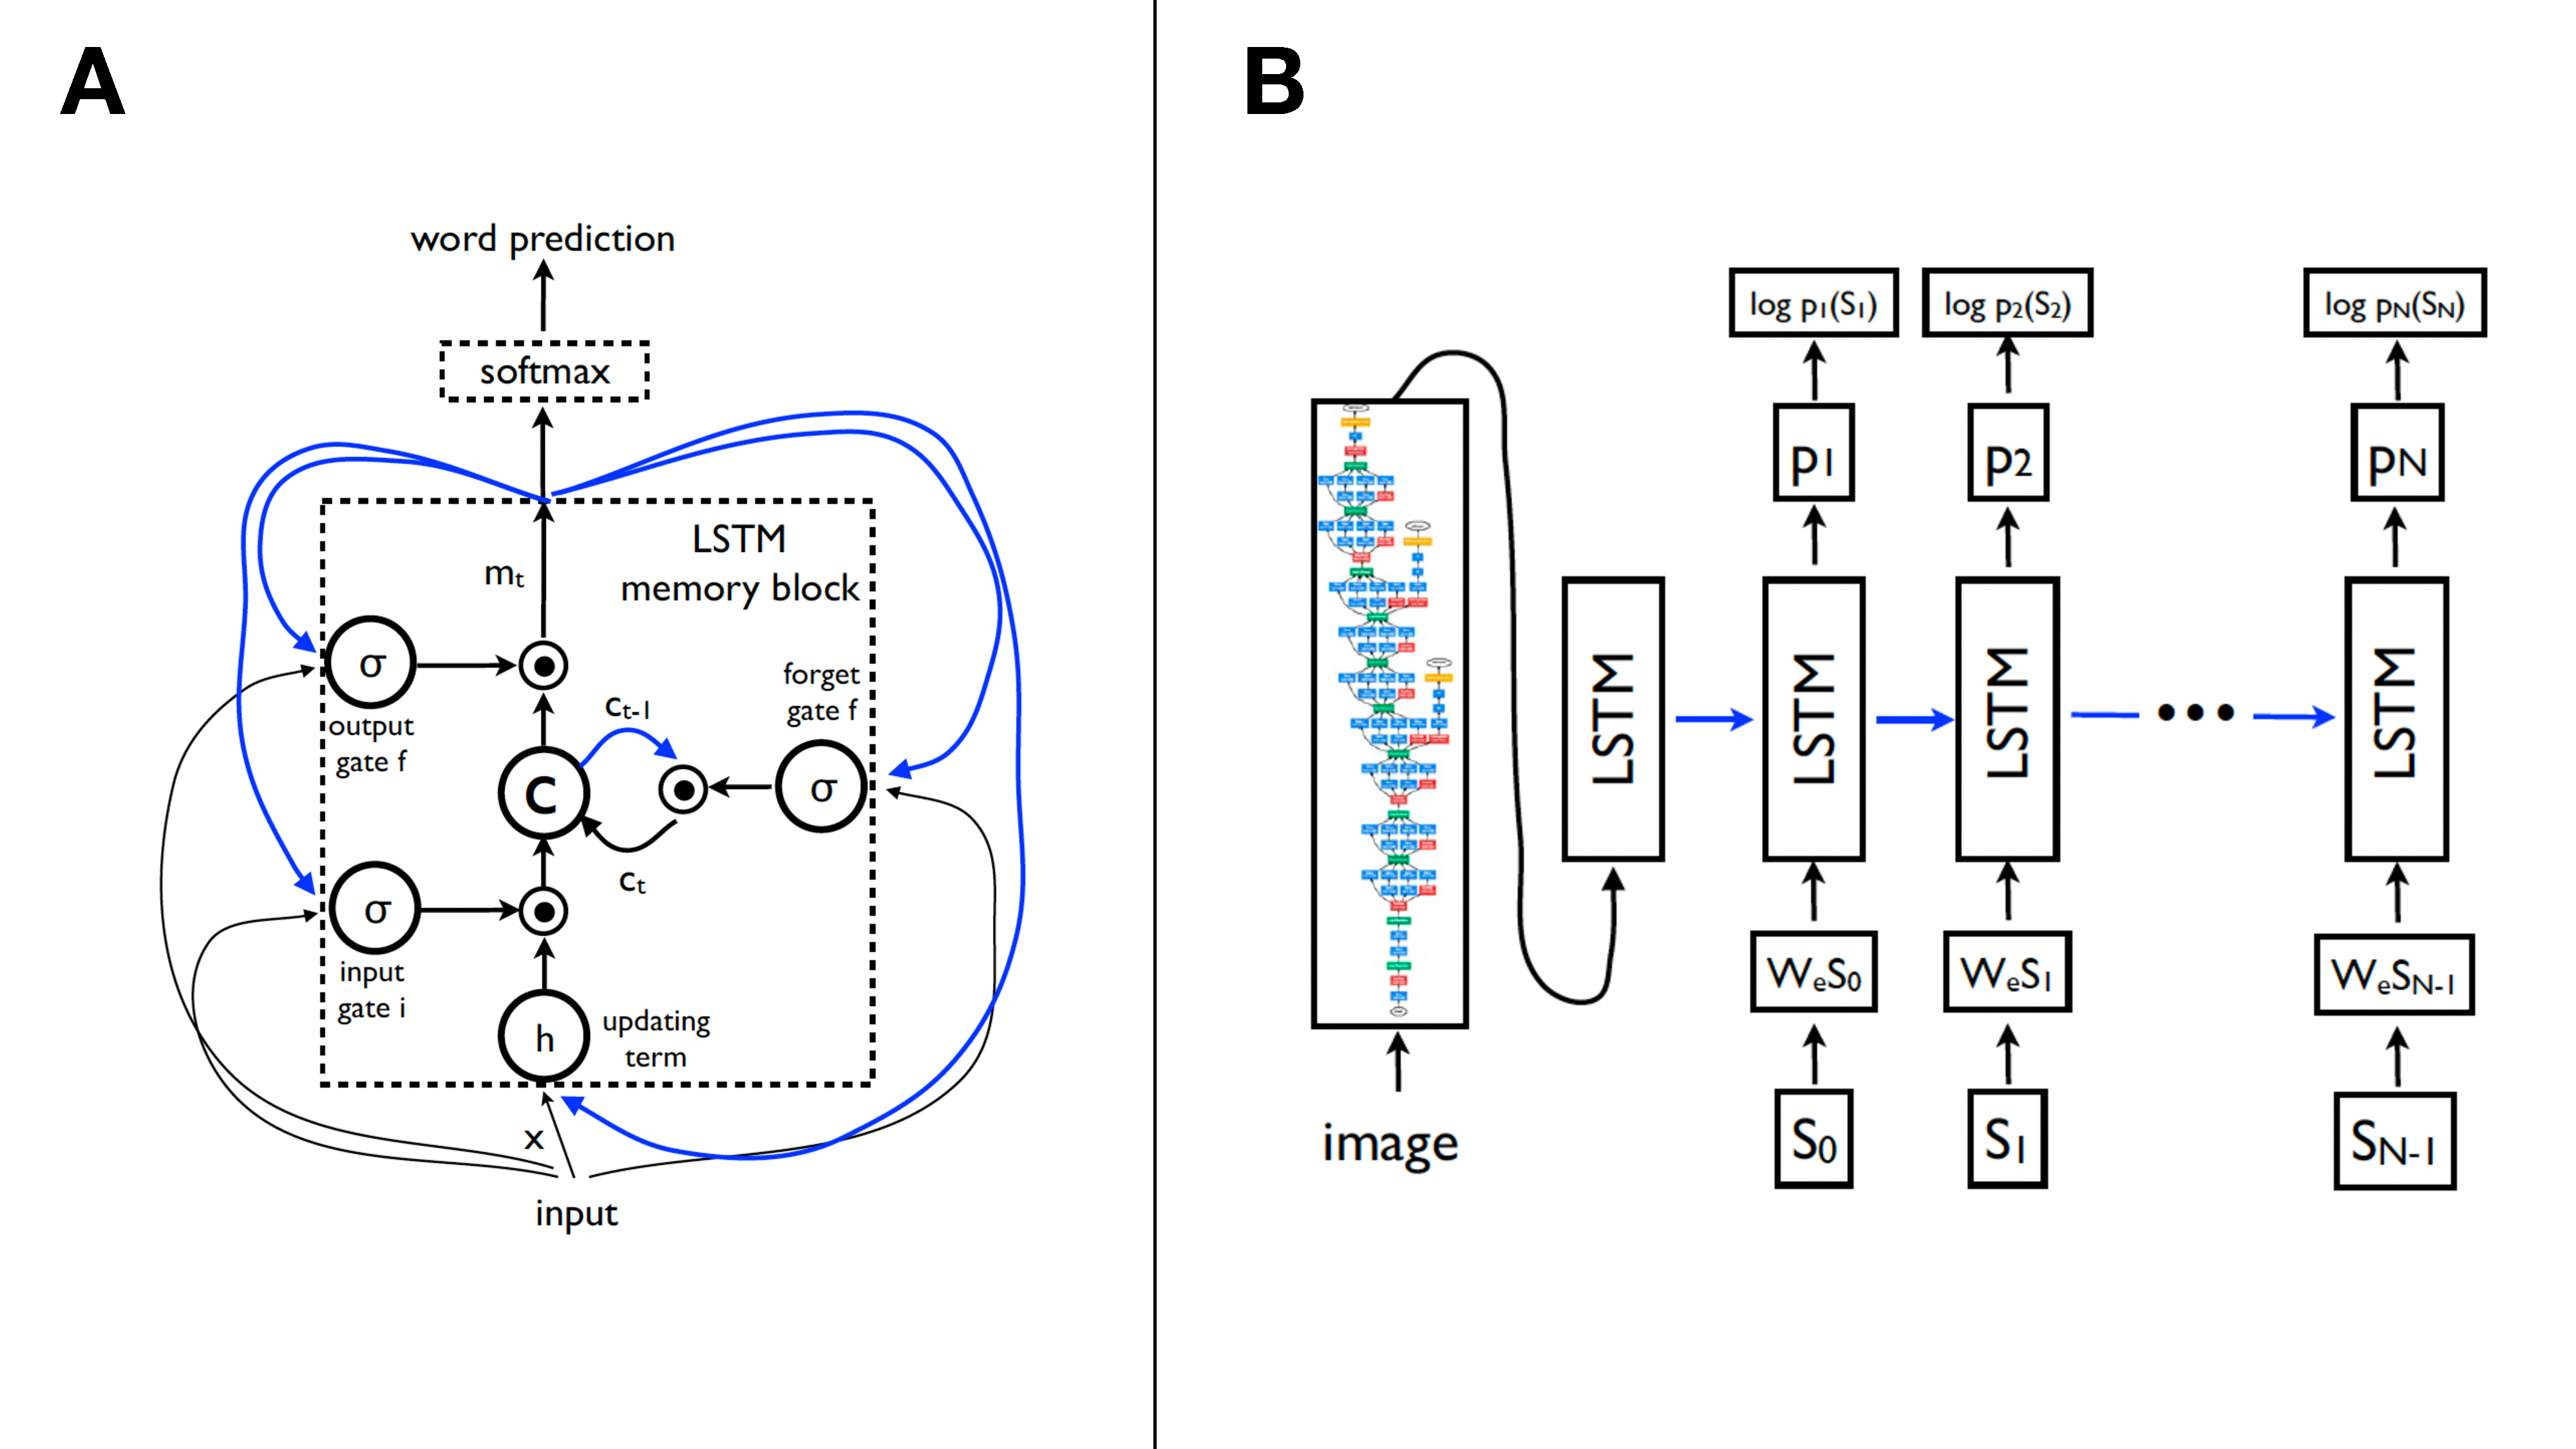
\includegraphics[width=\linewidth]{images/vinyals_lstm.pdf}
	\caption{A: LSTM cell architecture. B: Image captioner architecture consisting of a CNN image vector extractor (leftmost box) which passes an image vector into an LSTM cell (represented unrolled in time) as initialization of its hidden state. \parencite[][p. 2--3]{vinyals2015show}.}
	\label{fig:lstm}
\end{figure}

Another system was developed by \cite{karpathy2015deep}; the main idea of their architecture is to align parts of images with relevant parts of the respective caption. 
Their first system consists of a CNN pretrained on ImageNet which produces image embeddings, and a bidirectional RNN (BRNN) which produces embeddings of the corresponding captions in the same embedding space. Crucially, the BRNN is trained with a novel objective optimizing the alignment between ground truth captions and images via maximizing their dot product, while minimizing the dot product between images and incorrect captions. Using an additional  latent alignment variable the alignments produce sets of image regions annotated with (multi-word) phrases.
The learned alignments or full image-caption pairs are used as input data for a second image captioning model which consists of a multi-modal RNN. It is trained to generate image captions with a mechanism akin to the one by \cite{vinyals2015show}, but adding the image vector at the first time step of the sequence only. \cite{karpathy2015deep} conduct experiments on different datasets including MS COCO. Ranking experiments evaluating the first model showed intuitively plausible image-phrase alignments, next to improved results compared to then-state-of-the-art models. 
For evaluating the second model on full image captions, VGGNet image vectors were used, producing captions of decent quality as judged by standard evaluation metrics (see Table \ref{tab_coco_metrics_ref}). The model trained on region-phrase alignments was evaluated using human object annotations and was more consistent with those annotations than the full image model, indicating that the learned alignments were grounded correctly. In sum, their work is an interesting step towards generating captions based on more structured visual input.

\cite{xu2015show} propose a system where the image features are extracted using \textit{attention}, computed on annotation vectors representing parts of the image \parencite{bahdanau2014neural}. They compare stochastic attention to deterministic attention. The former is equivalent to the REINFORCE learning rule whereby the reward for the attention is proportional to the log likelihood of the target sentence (see Section \ref{rl_methods}). The latter is computed as a soft attention weight for the annotation vectors. This attention mechanism is diferentiable and, therefore, trainable end-to-end with back-propagation. The image location representation vectors were extracted using the VGGNet. For the experiment on MS COCO, they use a vocabulary size of 10.000; reported results are achieved with single models. The soft attention architecture allows to improve the test METEOR score on MS COCO by 0.02, while the hard attention does not yield an improvement, compared to \cite{vinyals2015show} (see Table \ref{tab_coco_metrics_ref}).

While the hitherto described systems consist of separate components used for representing the image and language parts, respectively, a different stream of work proposes \textit{joint multimodal} representations of images and captions. \cite{kiros2014unifying} learn a joint image-caption embedding space, using LSTMs for encoding the captions. Image representations extracted via a CNN are projected into the LSTM hidden states to create the multimodal embeddings. The multimodal embeddings are trained by maximizing cosine similarity between the image embedding and LSTM hidden state for the target image-caption pair, while minimizing the similarity to distractors. These multimodal embeddings are passed to a decoder module of various architectures which is then tested on image-sentence ranking and image captioning tasks. They show that multimodal embeddings outperform object-detection based models.

Guided by the idea of creating combined representations, the most recent architectural innovation in this domain applies transformer layers for creating unified vision-language representations, ommiting the use of separate CNNs and RNNs \parencite{vaswani2017attention, zhou2019unified}. This work is also motivated by advances achieved with pretrained language models, such that a growing body of work develops multimodal language models. The introduction of visual components in pretrained language models is also calles \textit{vision-language pretraining} (VLP).
Originally, VLP architectures were developed in the computer vision domain for image understanding tasks like visual question answering or image classification \parencite{zhou2019unified}. Crucially, the model is pretrained on image region embeddings combined with caption word embeddings in a transformer layer. Such pretraining is shown to be more effective on downstream tasks like image captioning after finetuning compared to non-pretrained architectures (see Table \ref{tab_coco_metrics_ref}: reported scores outperform all other models). \pt{Do a proper architecture summary here}
% so-called \textit{transformers} for this task. Transformers have been first applied to an image processing task by \cite{dosovitskiy2020image}. More specifically, 
% Vision-Language-Pretraining (VLP) domain of tasks - matching images to texts, trained with "masked language modeling objective on images and their aligned descriptions ".  

The experiments in this thesis closely follow the archtecture by \cite{vinyals2015show}. However, introduction of multimodal representation based models and more advanced networks as agents in multi-agent communication settings relying on visual input is an interesting direction for future work. 

\subsection{Model Pretraining}
\label{model_pretraining}
In this section, different approaches for training recurrent models which are predicting sequences, like the image captioning model is predicting a caption given the image, are discussed. In the context of multi-agent reference game experiments discussed in this thesis, this step can be seen as speaker agent pretraining.

It is assumed that the target task for the model is predicting the next token of a sequence, given the preceding tokens; this task is at the core of various applications like neural machine translation, image caption generation, text sumamrization and others \parencite[e.g.,][]{cho2014learning} \pt{	should be this: Sutskever, Ilya, Vinyals, Oriol, and Le, Quoc V. Sequence to sequence learning with neural network.} This task is usually modelled by recurrent neural networks \parencite{rumelhart1986learning}. The challenge when training recurrent neural network models which are predicting sequences at inference time by replicating the train time scenario, i.e., by conditioning the next token on the output of the model itself from the previous timestep, is slow convergence of the training, its instability and potentially poor generation skills \parencite{lamb2016professor}. The main training approach that has been proposed in order to mitigate these issues is \textit{teacher forcing} training, with several extensions to: \textit{search over candidate output sequences}, \textit{curriculum learning} and \textit{professor forcing} \parencite{goodfellow2016deep, williams1989algorithm}.

When using curriculum learning, at each step the source of input, i.e., whether it is the ground truth or the output of the previous timestep, to the next time step is chosen randomly \parencite{bengio2015scheduled}. This curriculum anneals over time, starting at teacher forced learning only (i. e., all inputs are ground truth tokens) and gradually transitioning to using predicted inputs. Among several decay schedules for the probability of the coin flip determining where the next input token comes from proposed by \cite{bengio2015scheduled}, inverse sigmoid decay schedule  was shown to yield best results on the MS COCO image captioning task.

When using professor forcing, the discrepancey between the training and inference performance is addressed by minimizing the discrepancy between the teacher forced and auto-regressive sampling behaviour, i. e., by making the distribution over sequences during training maximally similar to the target distribution \parencite{lamb2016professor}. This is achieved by training the model as a Generative Adversarial Network (GAN). More specifically, a second recurrent network---a biderectional RNN---  is introduced additionally to the RNN generating the captions. Due to the additional overhead for training an image captioner with this approach, exploring the effects of such pretraining on downstream multi-agent communication tasks is left for future work.

\pt{check entire paragraph} For conducting the experiments in this thesis, speakers pretrained with different following approaches are considered: pure teacher forcing pretraining, constant 0.5 rate teacher forcing, linear adaptive teacher forcing, scheduled sampling (with pure decoding, k = 30, ?) na topk sampling with a tenmperature of 2 (replicating \cite{lazaridou2020multi}). \pt{For details of selecting the final pretrained speaker, see XY. }

\subsection{Evaluation Metrics}
\label{image_cap_metrics}
An important yet non-trivial aspect of developing image captioning systems is their evaluation. Image captioning has been considered difficult to evaluate because for a given input image, several output captions might be equally suitable \pt{REF. Maybe example}. Therefore, usually a suite of evaluation metrics is used. This work employs the merics proposed for the MS COCO dataset \parencite{chen2015microsoft}: BLEU-$n$ ($n$ denoting the length of the n-grams), METEOR and CIDEr scores. In this section, conceptual aspects of these metrics applied to image captioning are introduced; for formal derivations, see, e. g., \cite{chen2015microsoft}.\footnote{The implementation of these metrics in Python provided by \url{https://github.com/daqingliu/coco-caption} is used in the present experiments.}

The BLEU-$n$ score evaluates the co-occurence on $n$-grams between generated and reference sequences \parencite{papineni2002bleu}. More precisely, the corpus-level $n$-gram precision is computed (fraction of relevant n-grams in the generated n-grams). That is, all reference captions are considered as a corpus, and the overall score is computed as a weighted geometric mean over all $n$-grams. However, BLEU favors short sentences and has been shown to be a poor metric for single sentence comparisons, especially when considering longer $n$-grams.

%The ROUGE metric was developed for text summarization evaluation and has three variations: ROUGE$_N$, ROUGE$_L$ and ROUGE$_S$. ROUGE$_N$ computes $n$-gram recall over all ground truth captions given the generated one (=fraction of found ground truth n-grams); ROUGE$_L$ is the $F$-score computed over the lengths of so-called \textit{Longest Common Subsequence} (i.e., an n-gram where other words may occur in between). Finally, ROUGE$_S$ is computed as $F$-score over counts of skip bigrams (i.e., bigrams where k words may occur in between).  Generally, the ROUGE scores are somewhat better at capture longer-range sentence structure preservation.

METEOR is computed by generating alignments between target and generated captions \parencite{banerjee2005meteor}. The alignments are based on both matching exact tokens and matching WordNet synonyms, stems and other generalizations. Then, the harmonic mean between the precision and recall over the best target-generated caption pairs, and the final score includes a penalty for quality of the found alignments. METEOR is computed as a corpus level metrics, as well, meaning that all target captions ar aggregated.
 
Finally, CIDEr is a native image captions evaluation metric \parencite{vedantam2015cider}. It is computed as a weighted TF-IDF for each $n$-gram occurring in the ground truth captions for the set of all images. Intuitively, the weighting provides a trade-off between common and distinctive n-grams. These weights are then combined into vectors for each n-gram of length $n$, based on which average cosine similarity between vectors for ground truth and generated captions is computed. The final CIDEr score is obtained as the average over the single n-gram similarities. In order to increase the similarity of metric results to human intuitions, further modifications including caption length-based gaussian penalties are included. Intuitively, CIDEr captures the similarity in distinctness or saliency of the generated and ground truth captions.

\pt{Recall based metrics usually reported.. seem to be related to the metrics including soome notion of recall?}

Since these metrics can only be computed in the presence of ground truth image captions, they are first and foremost applied in experiments on the MS COCO dataset, as experiments on the 3Dshapes dataset are based on self-generated ``ground truth'' captions and no reference values exist for this dataset.
Previous work on captioning the MS COCO datase discussed in this section provides a baseline for evaluating the quality of captions produced in this work. Table \ref{tab_coco_metrics_ref} provides and overview of scores achieved with extant systems.

\begin{table}[]
	\begin{tabularx}{\textwidth}{|X|l|l|l|l|l|l|l|}
		\hline
		Model                               & BLEU-1 & BLEU-2 & BLEU-3 & BLEU-4 & METEOR & CIDEr \\ \hline
		\cite{bengio2015scheduled}        & -      & -      & -      & 0.323   & 0.254  & 0.987 \\ \hline
		\cite{vinyals2015show}  & -      & -      & -      & 0.277    & 0.237  & 0.855 \\ \hline
		\cite{xu2015show} & 0.718  & 0.504  & 0.357  & 0.250     & 0.239  & -     \\ \hline
		\cite{karpathy2015deep}          & 0.625  & 0.450  & 0.321  & 0.230   & 0.195  & 0.660 \\ \hline
		\cite{zhou2019unified}          & -  & -  & -  & 0.365   & 0.284  & 1.179 \pt{?} \\ \hline
	\end{tabularx}
\caption{\label{tab_coco_metrics_ref}The table shows metrics results for the quality of captions generated on respective test sets of the MS COCO dataset. Best results reported in each paper are included.}
\end{table}

\section{Reinforcement Learning}
\label{rl}

Given the foundations of image captioning architectures, this section provides the tools for embedding these architectures into goal-directed interactive frameworks, like multi-agent communication.
\pt{Sift over italics and thelike. }

\subsection{Introduction}
A natural choice for training interacting artificial agents to complete certain tasks like language games is reinforcement learning (RL), as ``[r]einforcement learning is a computational approach to understanding and automating goal-directed learning and decision-making'' \parencite[][p.15]{sutton2018reinforcement}. Next to supervised and unsupervised learning, it represents one of three major paradigms in machine learning. 
%In this framework, the agents learn to make decisions as to which actions to take, given the environment, and receive responses to those actions from the environment putting the agents into new states . This repeats iteratively, until the agents learn how to effectively reach the desired goal state. For instance, the goal state can be understood as winning a game or successfully completing a communicative task. 
%``The reinforcement learning problem is meant to be a straightforward framing of the problem of learning from interaction to achieve a goal. The learner and decision-maker is called the agent. [...] These interact continually, the agent selecting actions and the environment responding to those actions and presenting new situations to the agent.'' (p.53). 
%A particular task is defined in terms of a complete definition of the environment, representing a particular instance of reinforcement learning (p. 54).

More precisely, reinforcement learning problems can be defined as learning the mapping from situations, represented as \textit{environments}, to optimal \textit{actions} that agents may choose in order to achieve task (sub-)goals, while maximizing the \textit{reward} signal \parencite{sutton2018reinforcement}. The reward can be understood as the environment's feedback about the optimality of the action with respect to achieving the goal (see Fig. \ref{fig:rl}). The chosen actions put the agent into new states. This repeats iteratively, until the agents reach the desired goal state or other interaction stopping conditions are met. For instance, the goal state can be understood as winning a game or successfully completing a communicative task. 

\begin{figure}
	\centering
	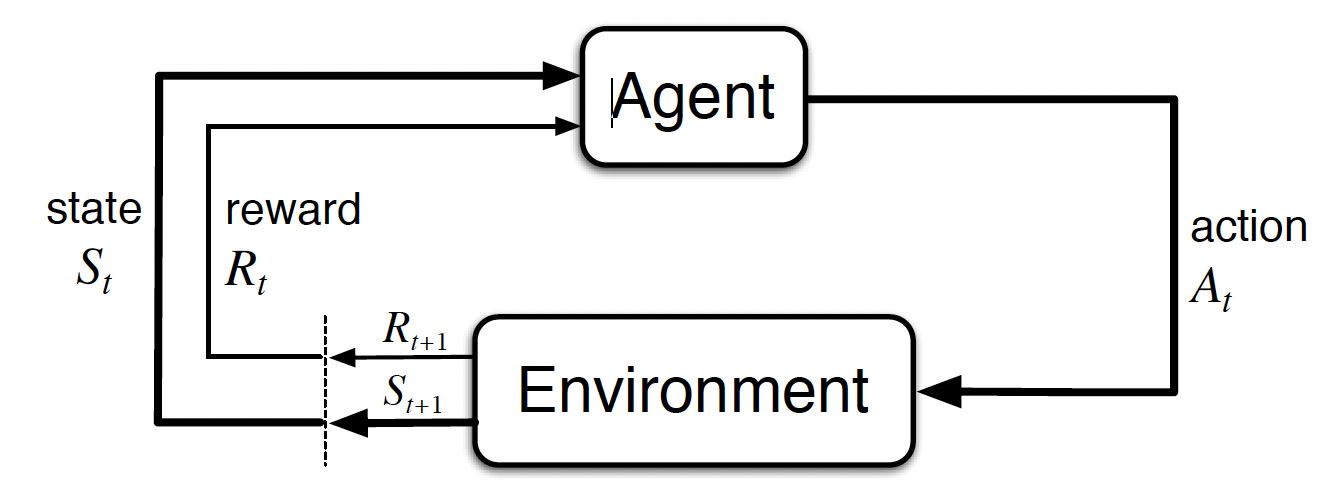
\includegraphics[width=0.8\linewidth]{images/rl_intro.png}
	\caption{Interaction of the environment with the agent via states, actions and rewards \parencite[][p. 48]{sutton2018reinforcement}.}
	\label{fig:rl}
\end{figure}

%The most important building blocks of RL systems are defined below: \pt{Definitions of: reward, environment, agents, actions, states, policy, value function, if necessary, q-learning maybe. An optiional model of the environment may also exist. }
% \begin{itemize}
%	\item agent: learner and decision maker in the interaction who tries to achieve a goal for a certain task.
%	\item environment: the setting in which the agent's interactions are situated, everything outside of the agent itself.
%	\item policy: the agent's learned mapping from environment states to actions within the environment. 
%	\item reward signal: \pt{TBD} numerical representation of the quality single \textit{rewards} the agent receives at each timestep of the decision process. Improtantly, the agents' goal is to maximize the sumn of the rewards over the task completion.
%	\item value function: a function mapping states to expected total reward for agents starting the actions at the given state. These are adapted and reestimated based on observed action and reward sequences of the agents over their lifetime. \pt{TBD}
%\end{itemize}

Decision making sequences modelled by reinforcement learning are standardly formalized as Markov Decision Processes (MDPs). 
It is assumed that the interaction takes place over discrete timesteps $t = 0,1,2 ...$.\footnote{Reinforement learning can also be applied to continuous state and action spaces. These aspects are ommitted in this introduction for brevity reasons.} At each step $t$, the state $S_t \in \mathcal{S}$ in which the agent is in can be considered as her current representation of the environment, where $\mathcal{S}$ is the set of all possible states. Given the state, the agent selects an action $A_t \in \mathcal{A}(s)$, where $\mathcal{A}(s)$ denotes the set of all actions available in state $S_t$ at timestep $t$. At the next timestep $t+1$, the agent receives a reward $R_{t+1} \in \mathcal{R}$ for the action $A_t$. These iterations can be formalized as \textit{finite} MDPs if they consist of an $\mathcal{A}, \mathcal{S}$ and $\mathcal{R}$ with finite number of elements. In this case, the probability $p$ for a particular state $s'$ and reward $r'$ to occur at time $t$, conditioned on the previous state and action, is well-defined \parencite[][p. 48]{sutton2018reinforcement}:  
\begin{equation}
p(s', r' \mid s, a) \doteq Pr(S_t = s', R_{t+1} = r' \mid S_{t-1} = s, A_{t-1} = a)
\end{equation}
Given $p$, one can then compute \textit{state transition probabilities} $\mathcal{T}$ (i. e., probabilities for reaching a particular state given previously visited states) 
\begin{equation}
p(s' \mid s, a) = \sum_{r \in \mathcal{R} } p(s', r \mid s, a)
\end{equation}
and, most critically, the expected rewards for given state and action combinations \parencite[][p. 49]{sutton2018reinforcement}: 
\begin{equation}
\E [R_t \mid S_{t-1}=s, A_{t-1}=a]
\end{equation}
The state transition probabilities and the function $p$, respectively, characterise the environment dynamics and, therefore, the MDP is modelled by the tuple $\langle \mathcal{A}, \mathcal{S}, \mathcal{T}, \mathcal{R} \rangle $. An assumption often made in the RL literature is that the states have the \textit{Markov property}, i.e., that they encode information from all previous interaction steps.

Expected rewards are especially important in order to estimate the \textit{return} $G$ and thus, formally represent the objective of learning---maximizing the return. In present work, the following simple definition of $G_t$ is assumed: 
\begin{equation}
G = R_{t+1} + R_{t+2} + ... + R_T
\end{equation}
where $T$ is the final step of the action sequence and $R_{t+1}$ represents the reward received for the action $A_t$. These interaction iterations yielding returns are also called \textit{episodes}. Different return formalizations, e.g., using expected discounted returns, are used in other applications for episodic tasks. However, a discount cannot really be applied in the present reference game scenario since the environment only provides one reward per entire episode (i.e., entire message generation; see below for details).

The mapping from actions and states to rewards is specified by the \textit{value function}. Since collected reward values depend on the taken actions, the last critical component of RL environments is the policy. ``A policy is a mapping from states to probabilities'' of taking available actions: $\pi(a | s)$ describes the probability that the agents chooses the action $a$ in the state $s$. The central problem of RL is then the estimation of an optimal policy, i. e., one yielding the maximal reward. The following section reviews different methods for estimating the policy, especially focusing on methods applicable to \textit{deep RL} \parencite{lecun2015deep}, i.e., RL with deep neural network agents akin to the ones used in present experiments. The overview is provided on a conceptual level, only providing more details for the algorithm used in the presented work.

%The central problem of RL is the estimation which action to take at each step in any state in order to maximize the return. To this end, in \textit{value-based approaches} the value function is estimated, which describes how valuable it is with respect to the expected return for an agent to be in a given state. 
%Terminal state = state at the end of each episode.
% Concrete specification and notation of actions, rewards, states and policy.
%Value functions and optimal policies (up to p. 95).
%Transition to deep reinforcement learning \parencite{lecun2015deep}.
\subsection{Deep Reinforcement Learning Methods}
\label{rl_methods}
Two main types of RL algorithms are usually distinguished in the literature: value based and policy gradient based methods. 

The main idea behind \textbf{$Q$-learning methods} is the construction of an action-value function called $Q$, making $Q$-learning a value-based method \parencite{sutton2018reinforcement}. The function is learned independently of the corresponding policy, although the learning proceeds via iterating over the steps of an episode and selecting actions according to a policy derived from the current estimate of the action-value function. In deep Q-learning, the function $Q$ is represented by deep neural networks \parencite[e.g.,][]{hester2018deep}. For an overview of different derivation methods, see \cite{sutton2018reinforcement}. 

The so-called \textbf{Actor-Critic method} also belongs to the class of value based methods, although both a policy and a value function are learned \parencite{sutton2018reinforcement}. It consists of an actor learning a policy from which the actions are sampled, and a critic, which is estimating the action value function of the currently used policy. The goal hereby is to estimate whether the action chosen based on the current policy improves the reward for the current state compared to its expected value. Based on the feedback from the critic, the policy is updated. 

In contrast, so-called \textbf{policy-gradient methods} focus on improving the parameters of the policy directly \parencite{sutton2018reinforcement, sutton1999policy, williams1992simple}. %More specifically, this approach provides a solution to the issue of computational intractability of analytically solving for an optimal policy (p. 80) and instead focuses on the agent's experience simulated from the environmant.  
More specifically, the policy is approximated stocastically with a parametrized function, e.g., a neural network. The policy is learned by optimizing the parameters $\theta$ of the model with respect to performance $\rho$ of the agent (e.g., rewards) at each step \parencite[][p. 1058]{sutton1999policy}: 
\begin{equation}
\Delta \theta \approx \alpha \frac{\partial \rho}{\partial \theta} 
\end{equation}
The \textit{policy gradient theorem} proves that this performance based gradient can be estimated even though rewards depend on explicit knowledge of the environment. It provides the derivation of an analytic expression which does not depend on the unknown distribution of states dictated by the policy and yielding the rewards. See \cite[][p. 326f.]{sutton2018reinforcement} for the formal derivation.

This introduction is constrained to a particular policy-gradient method---the algorithm REINFORCE---which is used in the presented experiments \parencite{williams1992simple}. For discussion of further policy-gradient methods, see, e.g., \cite{sutton2018reinforcement}. 
The REINFORCE algorithm posits that a locally optimal policy can be obtained by updating each weight $w_{ij}$ of the policy network accoring to 
\begin{equation}
\label{eq:reinforce}
\Delta w_{ij} = \alpha_{ij} (r - b_{ij}) \frac{\partial log(\pi)}{\partial w_{ij}}
\end{equation}
where $\alpha_{ij}$ is the learning rate, $r$ is the reward, $b_{ij}$ is the baseline (see below for details) and $\pi$ is the policy \parencite[cf.][p. 234]{williams1992simple}. The update depends on a gradient on the right-hand side; the policy gradient theorem shows that it is proportional to the expectation of a sample gradient. So when $r$ is available for each timestep including the last step of the episode, tractable weight updates can be computed retrospectively for the entire episode by applying \textit{Monte-Carlo} approximation. That is, the average over episode returns that are received based on observing an episode starting from an arbitrary policy and iteratively improving it are compute \parencite{sutton2018reinforcement}. Intuitively, the method selects weights proportionally to the expected return. One generally problematic aspect of Monte-Carlo methods is the behavior called \textit{exploitation} whereby actions that are selected more frequently are further sampled such that no information is learned about alternative actions. One way of maintaining sufficient \textit{exploration} (sampling new actions) is summarized below. 

Applied to sender agents in a multi-agent communication framework, the policy is the conditional probability distribution over message tokens, given previous tokens. The tokens are, therefore, the available actions. An episode is then the sampling of an entire message. The reward is the signal based on the task success, received upon producing the message. The goal is to learn to select the tokens so as to achieve the goal of the communication task with maximal rewards. Since the number of different tokens the agent may choose from at each timestep may be large in real-world application \parencite[cf.][]{he2015deep}, learning such an optimal policy remains a computationally difficult task.

One solution potentially stabilizing the learning in REINFORCE-based algorithms is the \textbf{selection of the baseline} $b_{ij}$ (cf. Eq. \ref{eq:reinforce}), which has been shown to significantly reduce the variance in many algorithms \parencite{sutton2018reinforcement}. 
Among other possibilities, the baseline can be represented by the running mean over the rewards, by a learned state value function, or a constant, and different studies investigate their effects on convergence speed and task performance \parencite{williams1992simple, greensmith2004variance}. However, upon initial exploratory simulations the addition of a mean baseline did not yield observable improvements of presented experiments and is, therefore, omitted in all conducted experiments. 

Another method for achieving more stable convergence of the policy is \textbf{entropy regularization} \parencite{williams1991function, mnih2016asynchronous}. More specifically, this method encourages the \textit{exploration} behaviour of the agents by encouraging the selection of states with high entropy, by adding a weighted entropy term to the policy based weight updates (cf. Eq. \ref{eq:reinforce}). The distadvantage of using entropy regularization is the introduction of an entropy weight as an additional hyperparameter to be tuned. However, it has been successfully used in practice and is also included in presented experiments.

The next chapter describes how the methods introduced in this chapter come together in work on multi-agent communication.

\pt{stationary distribution?}
%\pt{Add machine details in the expts section}
 
\chapter{Related Work}
\label{chapter03}

This chapter reviews related work on multi-agent communication---the core domain in which the presented experiments are situated. First, different architectures used for building the agent are reviewed. Then, different tasks the agents are trained on are summarized, focusing on the reference game setting. 
%Finally, the paper by \cite{lazaridou2020multi} which serves as the starting point for this thesis is summarized in detail.  

\pt{maybe find a way to say that there are other neighboring areas of research like visual dialogue, multimodal semantics, visual question answering etc. possibly in discussion.}

\section{Introduction}
Research on multi-agent communication has received increasing attention over the recent years, as this domain focuses on research questions of high relevance to cognitive science \parencite{lazaridou2020emergent}. More precisely, two main areas of research are often addressed: first, the conditions under which a language emerges and which emergent properties can be observed; and second, the ability of the agents to pick up a given language system. % thus investigating whether tractable human-agent communication channels can be learned via realistic interaction.
The second direction has also been considered with respect to \textit{grounding} a given language in the visual world. That is, approaches to teaching agents to use language applied to realistic visual input are investigated. Grounding is important both from modeling and cognitive perspectives: for instance, \cite{bruni2014multimodal} show that representations learned from both text and image data are more plausible than purely text-based representations; furthermore, vision is an integral part of human communication \parencite{tomasello2010origins, harnad1990symbol}. 

These two research directions have different implications for understanding human language: the former often focuses on what the causal factors behind prominent features of human language like compositionality are, allowing to shed light on human language evolution; the second rather addresses how we can train agents to communicate optimally for interacting with humans. Equivalently, these two main directions can be classified as investigating \textit{language emergence} and \textit{language acquisition} among and by artificial agents \parencite{lazaridou2018emergence, lazaridou2020emergent}.
Presented work focuses on the latter question, aiming to train agents to use English language grounded in real-world images.

Irrespectively of the research focus, artifical agents which interact with each other are at the core of multi-agent communication studies. Therefore, first, different agent architectures are presented in the next section.

\pt{I feel like a section on super general aspects, like having two agents doing some task and being jointly trained, is missing. Maybe visuals would be cool.}

Communication has been embedded in various tasks simulated in multi-agent settings. In some tasks like \pt{FILL ME} the idea is to use communication for more efficient cooperation and expertise transfer; in other tasks, communication itself is the core task. The latter allows to focus on properties of communicative systems that artificial agents might develop or acquire, thus allowing to compare them to human language. Since studying the ability of artificial agents to produce \textit{discriminative captions} for images in context within reference games is the goal of this work, this task and related work with human participants is described first, before transitioning to related work on multi-agent communication.

\pt{just to a section the chapter proceeds as follows and through out first paragraph and remove intro section.}

\section{Reference Games}
\label{reference_games}

Reference games are a type of the so-called \textit{Lewis singalling game} \parencite{lewis1969convention, skyrms2010signals}.
Signalling games were developed as an accont of \textit{conventional meaning} \pt{add def}. Traditionally, these games include two agents, a sender and a receiver. Only the sender observes a state sampled at random and chooses a message which is sent to the receiver. The set of possible messages is known to both agents. Based on the message, the receiver selects a state she chose based on the message. The game is a success if the guessed state and the state observed by the sender match, such that this game is driven by the agents having a common interest \parencite{lewis1969convention, franke2016evolution}. \pt{check if there might be a better reference}. 

\textit{Reference games} are then a specific instance of signalling games in which the meaning is already conventioanlly established. The sender samples a particular target among a set of distractors which may be a subset of all possible objects in the given world and \textit{refers} to it with her message. The target and the set of distractors are accessible to both agents. The receiver's task is then the identification of the target. Thus, the target and the distractors which are often represented by visual context in practice play a critical role in reference games.

Reference games have been employed in a wide range of studies with various research questions, often in order to study the pragmatic reasoning involved in generating referential expressions \pt{double check}. For example, \cite{franke2016reasoning} investigate whether pragmatic reasoning in reference games is population-level or individual. \pt{Def double check} For instance, \cite{graf2016animal} conduct an experiment wherein participants generate referential expression to a target image presented in context of distractors which either belonged to the same basic-level object category or to a different one.\footnote{\pt{define basic level categories and add reference, Rosch 1976}} They show that participants generated subordinate category, i.e., more specific, referential expressions in presence of more similar distractors, but not for dissimilar distractors. They show that humans flexibly increase the specificity of nominal expressions they use in order to unambiguously refer to the target, when required by the context. However, human speech also presents abundant examples of \textit{overmodification} in referential expressions, i.e., the use of additional modifiers like color expressions even when it is not strictly necessary for discrimination in the given conext. \cite{degen2020redundancy} explain this phenomenon in terms of complexity of the visual scenes, typicality of the referents and of the described features. They reveal complex pragmatic reasoning underlying this phenomenon. Much more work has been done on referential expressions both experimentally and theretically; these examples go to show that humans inherently generate highly discriminative, or, contrastive, messages in situations like reference games. Even further, they also expect and anticipate such behavior from other interlocutors, as has been shown in processing literature \parencite[e. g., cf.]{sedivy1999achieving}.

Applied to artificial agents, a reference game proceeds as follows: arrays containing a target image among $n \geq 1$ distractor images are sampled from the set of all images $I$. Both agents have access to the images and usually have the same representation; the sender agent knows which image is the target, the receiver does not. The sender emits a message $m, |m| \geq 1$ (assuming discrete communication; see Section \ref{multi_agent_arch}) sampled from the shared vocabulary $V$. Given $m$, the receiver has to correctly guess which of the images in the array is the target. Experiments in this thesis are limited to using one target image in context of only one distractor, but thy do not depend on this confinement.

\pt{Add Dale and Reiter, Computational interpretations of the Gricean maxims in the generation of referring expressions.  1995 }

\pt{Upshot: hypothesis about differing lengths as a proxy for different granularity of description. Bruni's paper as ground to believe that this might not be borne out as the bias in terms of length in the training dataset is too strong.}

\section{Discriminative Language Use}

Before turning to approaches wherein agents learn discriminative message generation in reference games, akin to human communication, rather machine learning-based approaches to building discriminative image captioning systems are reviewed.  \pt{it would probably make the most sense to review \cite{andreas2016reasoning} first, but then this framing doesn't quite make sense.}

\cite{sadovnik2012image} first approach discriminative image captioning by looking at visual discriminablity and saliency, and cosnstructing captions based on hand-crafted rules.

\cite{vedantam2017context} build an image captioning model which performs joint inference over a language model that is context-agnostic and a listener model which provides feedback on discriminativity of the captions. More precisely, they introduce a reaoning speaker consisting of a basic image captioning speaker and a listener model. The basic speakre is an image captioner pretrained on images and target concepts represented in the images. The listener is only dependent on the generative basic speaker, as it computes the log-likelihood ratio between the speaker's utterances for the same image but for different concepts. The overall speaker is the trained to maximize the basic generator probability while also maximizing the likelihood ratio represnting the discriminativity.
Thay apply the model to a justification task wherein the image feature corresponding to a given discriminative aspect of the caption has to be explained. They also apply it to standard image captioning on similar image pairs from the MS COCO dataset. They find that their architecture is able to generate caption which leads to higher discrimination success of human evaluators compatred to non-discriminative baseline.

\cite{dai2017contrastive} proposel the ``Contrastive Learning'' training objective for this task which constrains the image captioner to maximize the true caption likelihood compared to a pretrained reference image captioner, while learning to assign lower probabilities to mismatching caption for the target image, compared to that same reference model. Critically, the success of the system depends on the quality of the reference model. Their model achieves competitive results on the MS COCO test set.

While alleviating some issues like language drift \pt{check if it is okay to foreshadow this here like thsi}, these systems miss a critical component in the approach to the task---they are missing the communicative and interactive context of applying such cpations. Yet interactivity and social aspects of the communicative task are critical for developing systems which are supposed to be able to adequatly interact with humans. The arguably most prominent framework formalizing social and cooperative aspects of communication is the Rational Speech Act (RSA) framework \parencite{goodman2016pragmatic}. Some approaches to discriminative image captioning are highly inspired by RSA and thereby incorporate interactive communicative aspects into their models.\footnote{Basic knowledge of the RSA family of models is presupposed. For a gentle introduction, see, e.g., \cite{problang}.} \pt{double check adjectives here}

\cite{andreas2016reasoning} are the first to employ an RSA-style Bayesian model wherein the agents learn to produce discriminative messages in a reference game by reasoning about the other agent. They also use the Abstract Scenes dataset. The architecture consists of a base speaker, base listener and a reasoning speaker. All agent modules are based on fully-connected linear layers with non-linear activations. The literal listener consists of modules embedding input images and the received message, and computing scores over image-message pairs. The literal speaker is used to sample possible messages for a given image by computing scores over vocabulary tokens given the image with a feed-forward conditional language model. The reasoning speaker then derives the optimal message by sampling candidate messages from the literal speaker and reasoning about their utility by ``passing'' them through the literal listener and choosing the message maximizing the listener's referential success probability. 
\cite{andreas2016reasoning} found that referential success increases with the number of samples taken from the literal speaker, as well as with increasing weight of reasoning about the listener in the reasoning speaker model. Further, they find that the reasoning speaker outperforms the literal speaker, indicating that pragmatic reasoning might be crucial for modeling task-conditional language use. \pt{seems highly relevant to my intuition about regularization and strucutral weight. add to discussion.}

\cite{cohn2018pragmatically} also build a model following the standard RSA architecture. Their model performs character-wise caption generation in order to constrain the space of possile alternatives the speaker may choose among when generating the caption. Therefore, their generation process is an incremental one, modelled by an LSTM-based speaker agent. Their model  turns out to outperform word-level generation and non-pragmatic models. \pt{see if we want more detials}

\cite{nie2020pragmatic} propose an issue-sensitive image captioner, also based on the RSA famly of models. Issue-sensitivity is represented as partitioning  the space of images into cells with images having the same relevant (i.e., at-issue) feature as the target. Their base speaker is a standard  pretrained image captioning model. Additionally to standard RSA mechanics, they extend the pragmatic speaker to be sensitive to the relevant partitioning. They further include a utility term in order to tackle arising semantic drift (e. g., mentioning features that are not true of the target) of the captions and constrain the speaker from overgenerating. This model also employs an incremental speaker generation procedure. Evaluations include visual question answering (VQA) on MS COCO, showing that the model learns adequate issue representations from questions as well as generates promising issue-sensitive captions. 

Finally, an approach fully embracing the idea of learning language use from active interaction, not just representations of other agents,  is multi-agent communication. Therefore, the next section turns to work on discriminative language learning and other related research in this domain.

\section{Multi-Agent Communication}
\label{mac}
The main architectural differences concern the type of model representing the artificial agent and the type of communication channel they use.
As described in Section \ref{rl}, experiments wherein agents learn to complete a task by interacting with the environment and with each other are typically trained with reinforcement learning. Multi-agent communication is a specific type of such experiments in that (one of) the tasks agents learn are communicative and cooperative, and one of the agents can be considered the sender and the other the receiver of the communication \parencite[cf.][]{tan1993multi, lazaridou2016multi}.
Based on the chosen communication channel and the precise communicative task, specific architectural decisions and optimization algorithms differ. 

\subsection{Agent Architecture and Training in Reference Games}
\label{multi_agent_arch}

While early work in multi-agent communication focuses on structured agents \parencite[e. g., see][for reviews]{christiansen2003language, cangelosi2002symbol}, deep agent architectures became increasingly dominant in the domain over the last years \parencite{lazaridou2020emergent}. As this thesis also uses deep neural network agents, the review of related work focuses on deep multi-agent communication experiments. 

%Architectural considerations: 
%1) agent architecture: hand crafted vs deep; for deep: kind of network, esp. recurrent layer
%2) loss and training approach: Q-learning \parencite{foerster2016learning}, Gumbel-Softmax \parencite{havrylov2017emergence}, REINFORCE.  \parencite{lazaridou2020emergent, williams1992simple}. 

\cite{lazaridou2016multi} first show that neural agents can efficiently reference realistic visual inputs in the presence of distractors by developing a communication protocol from scratch. To this end, \textcite{lazaridou2016multi} conduct several experiments employing feed-forward and CNN agents. In particular, in their main experiment, they set up a reference game, where a sender agent emits a single discrete symbol referring to one of two images provided to both the sender and the receiver, sampled from the ImageNet dataset \parencite{deng2009imagenet}. The discretization of the agents' communication channel is sometimes also called the \textit{discrete bottelneck} \parencite{lazaridou2020multi}. 
The receiver agent has to guess  which image is the intended target, based on the symbol received from the sender (see Section \ref{reference_games} for details). %They use a subset of the dataset containing 100 images from each of 20 general categories.
\cite{lazaridou2016multi} set up two versions of the sender. The ``agnostic sender'' consists of a two-layer feed forward neural network, embedding both images and producing a score over the vocabulary given the concatenation of image embeddings \parencite[][p. 3]{lazaridou2016multi}. The ``informed sender'' consists of a three-layer neural network, applying two convolutional layers to embeddings of both images which are treated as different channels \parencite[][p. 3]{lazaridou2016multi}. It also outputs scores over the vocabulary. For both architecures the scores are converted into a Gibbs distribution from which the emitted message symbol is sampled. The receiver agent consists if a two-layer feed forward network which embeds both images and computes the dot products between these embeddings and the one-hot encoded message. The final target image choice is sampled from the Gibbs distribution computed from the dot products. %The agents are trained with REINFORCE which updates parameters of the speaker and listener policies by minimizing the negative expected reward. The speaker and listener policies are parametrised by the weights of the respective neural networks. The sender policy is $\pi(v \in V \mid i_L, i_R, t \in \{L, R\})$ where $V$ is the vocabulary, $i_L, i_R$ are the left and right images and $t$ is the position of the target. The receiver policy is $\pi(t \in \{L, R\}\mid v_s, i_L, i_R)$, where $v_s$ is the message received from the sender and $t$ is the guessed position of the target image. \textcite{lazaridou2016multi} set the reward to 1 if the image picked by the receiver is the target and 0 otherwise. 
They found that agents achieve high referential success, and that the informed sender produces semantically more natural symbols (i.e., the same ones for the same image categories) than the agnostic one. In a further experiment, the authors successfully pressure the agents to communicate about more high-level properties by sampling instances of different subcategories within the same basic-level category for the image pairs.%, and achieve a small increase in label purity (i. e., in the proportion of labels agreeing with the major cluster label). 
Finally, they perform an experiment grounding the communication in natural language wherein the sender agent has to use natural language category labels as message symbols. The sender is trained by switching between reference game play and image classification on ImageNet data. However, the vocabulary is limited to 100 words, and the sender only produces one-word messages. %They observe a higher symbol purity in this experiment, while retaining referential success. 	
%	\item They use REINFORCE for training the speaker. Overall framing: interactive communicative setting for training agents allows to capture functional aspects of communication, i.e., the goal-directed nature of communication, as opposed to purely supervised conversational agent training. 
%	\item \textit{multi-agent coordination communication game}: first functional task (a basic function of language): reference
	
Another foundational study in deep multi-agent communication was conducted by \cite{foerster2016learning}. In contrast to \cite{lazaridou2016multi}, the authors let the agents use a centrally trained system in their ``DIAL'' architecture (i. e., with parameter sharing across agents)  which can also be extended to continuous communication. This system is compared to the ``RIAL'' system where agents use traditional discrete communication \parencite[][p. 2]{foerster2016learning}. This is one of the first studies using a recurrent network in the sender architecture.
For both systems, the sender consists of an input network with a fully connected layer and lookup tables creating embeddings of the task environment, two recurrent GRU layers, and two feed-forward output layers.
The receiver has the same architecture. The DIAL agents are connected via a continuous vector which can be seen as an activation layer passing the internal state of the sender to the receiver.
Experiments with different variants of a riddle task and an image classification task on the MNIST dataset were conducted. Results on the former task show that the agents were able to learn an optimal policy although DIAL agents converged faster, yet sharing the weights between the sender and receiver agents was critical for RIAL. DIAL with parameter sharing outperformed other experiments. Furthermore, they found that adding noise to the communication was critical for successful learning for RIAL. Results of the second task provided similar results for DIAL, while RIAL failed to converge stably on the multi-step interaction version of this task. 
The discrete system is trained with deep $Q$-learning (see Section \ref{rl_methods}), while the continuous system was trained by additionally backpropagating gradients end-to-end between the two agents. %Furthermore, the former but not the latter case includes modeling wherein agents have access to each other's internal representations of the environment, which was also argued to be unnatural when developing a system to investigate human communication \pt{REF}. 
The DIAL results pose an interesting question regarding the comparability of such a system where the internal representations of a speaker are directly passed to the listener to human communication \parencite[cf.][]{lazaridou2020emergent, hockett1960origin}. The authors, however, argue that this direct error propagation can be interpreted as communicative feedback which is also part of human communication. Further, while the possibility to use DIAL with continuous communication is attractive from a machine learning perspective due to its straightforward differentiability, human languages are typically considered discrete signalling systems \parencite{hockett1960origin}. 

\cite{havrylov2017emergence} further extend work on multi-agent communication by modeling agents which  communicate with variable-length strings of symbols in a reference game. 
Their architecture is based on the proposal \cite{lazaridou2016multi} with the difference that the sender agent only has access to the target image. Furthermore, their agents consist of LSTM layers. Information about the target image is injected by initializing the hidden state of the sender LSTM with the image feature vector, extracted from a pretrained VGG CNN. The sender generates the message by sampling tokens from the vocabulary similarly to the image captioning system by \cite{vinyals2015show} described in Section \ref{image_captioning}. The vocabulary consists of 10,000 tokens, the LSTM hidden size is 512, and the token embeddings are 256-dimensional. 
The receiver interprets the message by encoding it with the LSTM and computing a probability distribution over dot products of image features and the affine-transformed hidden state of the LSTM. The image with the highest probability is chosen as the target. \cite{havrylov2017emergence} further attempt to make the statistical properties of the emergent protocol as similar to natural language as possible by minimizing the KL-divergence between the learned conditional token distribution and a pretrained language model.
They compare agents trained via the \textit{straight-through Gumbel-softmax estimator} to agents trained with REINFORCE. The straight-through Gumbel-softmax estimator is a differentiable approximation of discrete actions (i. e., tokens) with a continuous relaxation applied in the backward pass of the backpropagation, while still using discrete representations in the forward pass. 
That is, one-hot encoded tokens are replaced with samples $w_k$ obtained by sampling $K$ samples  $\{u_k\}_{k=1}^K$ from the random variable $u \sim U(0,1)$. Each $u_k$ is transformed and then used in the sample computation:
\begin{equation}
\begin{aligned}
g_k = -log(-log(u_k)) \\
w_k = \frac{exp((log \; p_k + g_k) / \tau)}{\sum_{i=1}^{K} exp((log \; p_i + g_i) / \tau)}
\end{aligned}
\end{equation}
where $\tau$ is the temperature, $p_i$ and $p_k$ are token probabilites. The samples are discretized with argmax for the forward pass. Thus, it is an alternative to REINFORCE in this setting.
It is argued in the literature that this approximation allows more efficient gradient estimation given larger action spaces for which REINFORCE produces very high variance estimates, e. g., when the vocabulary size is larger \parencite{havrylov2017emergence}.

Experiments on the MS COCO dataset are conducted, selecting one image in batches of 128 as the target. They showed that agents trained with Gumbel-softmax converge faster than those trained with REINFORCE, but both are able to achieve high referential success. Further, they find that communication success increases with maximum message length for both algorithms. They also find that the emergent communication protocol has multiple representations of the same information and that the messages seem to have hierarchical coding. They also conduct an experiment wherein the sender is trained with a combined loss on both an image captioning and reference game task in order to attempt to grounding the tokens in the images. However, this system didn't improve in terms of caption quality. To sum up, this work showed that agents can successfully develop multi-token communication protocols for solving referential tasks.

Similar work is conducted by \cite{lazaridou2018emergence}. The agent architecture closely matches \cite{havrylov2017emergence}, yet the study focuses on comparing reference games with realistic images to games on symbolic data. The protocol learned on symbolic data was shown to exhibit higher topographic similarity to the input data and more compositional features compared to raw pixel input experiments. Nevertheless, agents were able to successfully develop a protocol based on raw input, as well. These results suggest that the proposed architecture does not have an inductive bias sufficient for extracting symbolic compositional features from raw inputs. 

\cite{lazaridou2020multi} whose work is replicated and extended in this thesis use an architecture which combines the architectures by \cite{lazaridou2016multi} and \cite{havrylov2017emergence} in that they also use LSTM based agents, but condition them on combined image features of both the target and the distractor. That is, they conduct reference game experiments with pairs of images. They explore different speaker architectures. More precisely, they compare a speaker learning an emergent communication protocol maximizing the reference task success (``functional learning''), a speaker learning to emit images captions as messages based on ground truth captions in a supervised manner (``structural learning''), and speakers trained with a combination of the two learning approaches \parencite[][p. 4]{lazaridou2020multi}. The functional learning signal is also based on REINFORCE, while the structural learning is conducted with the standard cross-entropy loss. Multiple combined speaker parametrizations are compared: a speaker pretrained on an image captioning task which is then fine-tuned with functional learning on the reference game (conditioned on the target image only) (``reward finetuning''), a speaker trained with a weighted combination of the structural and functional losses (``multi-task learning'') and a speaker pretrained on image captioning and then learning a reranking function based on the reference game (``reward-learned rerankers'') \parencite[][p. 4--5]{lazaridou2020multi}. Two variations of the reranking model are presented; both speakers learn to rerank samples obtained from a pretrained image captioner. The ``product of experts reranker'' reranks the samples proportionally to the message probability times the probability of the message given the image pair. The latter is obtained by re-embedding the sampled captions with a trainable layer as bag-of-words vectors and computing dot ptoducts between the vectors and image embeddings, renormalizing the scores.  The ``noisy channel reranker'' learns the reranking according to Bayes rule, i. e., proportionally to the likelihood of obtaining the target image given the sample times the sample probability. The likelihood can be seen as the speaker's internal listener model and is also computed as the re-normalized dot product between a learned bag-of-words caption representation and each image embedding \parencite[][p. 5--6]{lazaridou2020multi}. The agents were trained on a reference game on the \textit{Abstract Scenes} dataset.
They showed that the ``product of experts reranker'' model outperforms other speakers with respect to referential success in the game, while also counteracting language drift (see Chaper \ref{chapter04} for details). 

More specifically, they conduct a set of evaluations: they evaluate the different trained speakers trained simulataneously with a listener against the same joint listener, a fixed pretrained listener and a human, using an easy and difficult test set consisting of 1000 image pairs each. Furthermore, they vary the source of the samples for the reranker models: they are either the ground truth captions or samples from an image captioner pretrained on single image captioning only. As a baseline, they have human speakers pick the most discriminative caption among the ground truth options for a human listener and achieve an acuracy of 0.97. By contrast, an oracle reranker model operating on the ground truth captions learned against a joint listener only achieves an accuracy of 0.92 with human listeners, indicating that the capacity of the listener and reranker modules are somewhat below human performance. They find that the noisy channel speaker performs best ith humans when trained with a joint listener, while the PoE model performed best with humans when reranking ground truth captions. Investigating the reasons for language drift, they find that the speaker-listener co-adaptation has the least effect on the noisy channel speaker (human performance 0.86 vs 0.87 for joint vs fixed speaker training), and most significant effect on the the reward finetuning with KL speaker (human performance was 0.69 vs. 0.0.75). Finally, they find dthat unfreezing the visual model weights increses the gap between the performance of the joint and human listeners when training the reranker with a joint listener on with ground truth captions. 

Experiments in this thesis focuses on the ``multi-task learning'' architecture. This choice is discussed in more details in Chapter \ref{chapter05}.
\pt{make sure to describe in detail the results of easy-difficult comparison and tests against oracle speakers.}

%The noisy channel reranker model by \cite{lazaridou2020multi} is closely related to work by \cite{andreas2016reasoning}. They also employ a Bayesian model wherein the agents learn to produce discriminative, i. e., task-directed grounded messages in a reference game by reasoning about the other agent. They also use the Abstract Scenes dataset. The architecture consists of a base speaker, base listener and a reasoning speaker. All agent modules are based on fully-connected linear layers with non-linear activations. The literal listener consists of modules embedding input images and the received message, and computing scores over image-message pairs. The literal speaker is used to sample possible messages for a given image by computing scores over vocabulary tokens given the image with a feed-forward conditional language model. The reasoning speaker then derives the optimal message by sampling candidate messages from the literal speaker and reasoning about their utility by ``passing'' them through the literal listener and choosing the message maximizing the listener's referential success probability. This architecture is closely related to idea of Rational Speech Act models \parencite{goodman2016pragmatic}. 
%\cite{andreas2016reasoning} found that referential success increases with the number of samples taken from the literal speaker, as well as with increasing weight of reasoning about the listener in the reasoning speaker model. Further, they find that the reasoning speaker outperforms the literal speaker, indicating that pragmatic reasoning might be crucial for modeling task-conditional language use. \pt{seems highly relevant to my intuition about regularization and strucutral weight. add to discussion.}

\cite{lee2019countering} use another architecture---an attention based sequence-to-sequence machine translation model with one GRU layer---for both agents. 
The agents play a multi-modal translation game wherein the first agent is tasked with the translation of a sequence from French to English and the second---from English to German. Both agents are pretrained on the translation task before the communication game. This setup is used in order to investigate \textit{language drift} of the pivot language English, i. e., its deterioration (see Chapter \ref{chapter04} for details), as the agents are trained on French-German translation with REINFORCE (see Chapter \ref{chapter02} for details). They compare the mitigation of language drift through a language modeling constraint (i. e., incorporating the maximization of the likelihood of the English sentence under a pretrained LM into the reward) to grounding (i. e., maximizing the likelihood of an image corresponding to the English sentence under a pretrained image retrieval model). The LM is a one-layer LSTM; in the grounding model, image features are extracted using a pretrained ResNet-152. \cite{lee2019countering} find that the agents are best able to learn decent French-German translation when mitigating language drift with both an LM constraint and grounding. \pt{check italics of language drift and reference to chapter 4 thru chapter}

\subsection{Other Tasks}

Next to studying communicative success and the ability of agents to use natural language in reference games, multi-agent communication work has also focused on other aspects in reference games as well as studied other tasks.
 
For instance, \cite{evtimova2017emergent} extend the one-iteration reference games to \textit{multi-step interactions}, wherein agents can exchange information back and forth several times. More specifically, their sender agent only has access to visual representations of the set of objects, while the receiver only has access to textual descriptions of the target and distractors. Therefore, the agents need to align their communication across modalities. They compare a feed-forward and an attention-based sender architecture, and a GRU-based and attenion-based receiver, training them with REINFORCE. They find that agents successfully make use of back-and-forth communication about ImageNet images with WordNet based descriptions, showing that agents produce longer conversations on more difficult concepts. Further, they observe an increase in sender's message specificity with progressing conversation iterations.
Their experiments are also related to the multi-step MNIST task variation of \cite{foerster2016learning}.

A further step is taken by \cite{bouchacourt2019miss} who model a decision task wherein one agent is assigned a fruit and the other two tools, the latter having to decide which tool is more suitable for using with the given fruit. The tool utility is retrieved from human judgements. Noteworthily, the type of objects assigned to an agents is varied at random. They observe that the agents develop role-dependent communicative protocols. 

Other work studies the communication in more complex cooperative environments like 2D or 3D grid worlds \parencite{das2019tarmac}. In contrast to other studies, they use the Actor-Critic training method and continuous communication protocols. In short, they find that the benifit of including communication increases with task complexity, and that the learned communication and underlying agent behaviour are intuitive and interpretable. However, \cite{lowe2019pitfalls} also highlight the difficulty of adequately evaluating the added value of communication in complex multi-agent environments.

Finally, a body of work focuses on investigating the properties of emergent languages with the goal of understanding how natural language properties might have developed \parencite{lazaridou2020emergent}. For instance, \cite{graesser2019emergent} show, among other findings, that a shared communication protocol emerges from distinct ones in presence of a single new agent in the community participating in the communication. This presents an important connection to natural language which largely preserves its structure precisely because of the pressure to communicate with different interlocutors and culturally transmit the language to further generations. \pt{reference! and check!} \cite{chaabouni2019anti} investigate whether emergent communicative protocols follow Zipf's law positing that freuquency of messages in a language is anti-correlated with message length. Surprisingly, they find that emergent protocols are \textit{anti-efficient}---that is, the messages that have to be used most frequently are the longest ones. This is explained by a lack of production cost pressure in emergent communication.

Similarly, driven by investigating properties of natural language, a lot of work has focused on \textit{compositionality}.\footnote{Measuring compositionality is an important and not trivial aspect of this line of work. For an overview of different approaches, see, e.g., \cite{lazaridou2020emergent}.} For instance, \cite{lazaridou2018emergence} show that compositional communication emerges more easily from symbolic input than raw pixel input. 
\cite{chaabouni2020compositionality} show that compositionality in emergent protocols facilitates language transmission, but is not predictive of its generalization potential. The emergence of compositionality is shown to be strongly dictated by the variability of the input environment. Importantly, they also use a structured symbolic input representation.
This is in line with the observation made in human experiments and grounded in theoretical work that ``generational transmission of language favors compositionality'' (\cite{lazaridou2020emergent}, p. 12; cf. \cite{kirby2014iterated}).
\cite{luna2020internal} investigate cognitively plausible internal and external pressures which might influence compositionality---the ``principle of least effort'' (i.e., keeping the messages as short as possible) and ``object constancy'' (i.e., grouping together constant patterns into conceptual classes by abstracting away from context-contingent variation) (p. 1). More precisely, operationalizations of the latter principle in terms of sensitivity towards location invariance, color constancy and the distribution of objects in the environment are compared. The results show that the least effort pressure makes the protocols less redundant. Furthermore, agents pressured towards object constancy produce protocols with highest compositionality scores, while some operationalizations also improve zero-shot generalization abilities. 

To sum up, these studies show that emergent communicative protocols often exhibit properties that are far from natural language. Nevertheless, the ability to test the effect of different environmental and architectural pressures on emergent properties makes multi-agent communication a fascinating avenue for further research. 
%Other evolutionary perspective: agent co-evolution \parencite{dagan2020co}.

%\textbf{Properties of the communication \parencite{lazaridou2020multi}}: difficulty to converge on consistent meanings of tokens for color values, generally task-oriented codes with complexity minimization. Anti-efficient code development --> I am looking somewhat into this with my different-lengths experiments and grammars.  Larger communities lead to more systematic languages --> fixed listener experiment.

\pt{it would be good to have something with different listeners, i e the cultural transmission aspect.}
%Compositionality. also paper by Bruni.

\pt{Don't forget chapter summary.}

\chapter{Investigating Language Drift}
\label{chapter04}
This section describes the data used in the present experiments, the architecture of the agents, experimental procedures, as well as results. There are two agents---the speaker and the listener agents---whose architectures are shared across all experiments and, therefore, described once. At first, the general set up of the reference game common to all experiments is described, while experiment-specific details are provided in the respective sections.  

\section{Datasets}

Sources.
\subsection{MS COCO}
Descriptive stats, splits that were used.
\subsection{3dshapes}
Descriptive stuff.
\subsubsection{Caption Generation}
Procedure. 

\section{Reference Game}

The current experiment are limited to using one target image in context of only one distractor, but the current experiment do not depend on this confinement.

\section{Architecture}
The architecture of the agents follows \textcite{lazaridou2020multi}, except minor details to be explained below. \textcite{lazaridou2020multi} explore different ways to parametrize the speaker agent, and the current work replicates the ``multi-task learning'' parametrization (p. 5). This choice is motivated by the fact that among their architectures, this is the only one where the speaker agent learns to produce messages and its core image captioning capability while having access to both the target and the distractors, as opposed to models relying on sampling captions from a pretrained single-image captioning models.\footnote{I think that the multi-task learning set up by \textcite{lazaridou2020multi} really doesn't use pretraining---see their Appendix A ResNet module note.} 

Both agents have two components: a visual embedding module which takes as input the target and distractor images, and a language module. More specifically, the visual module for both agents embeds image features which were extracted using the same pre-trained ResNet50 model \parencite{he2016deep}. The weights were accessed through the \texttt{torchvision.models} API \parencite{marcel2010torchvision}. Features from all images of the dataset were extracted and saved and then retrieved when training all agents. 
The language module differs for the two agents, so details are provided below. 
The code for all experiments can be found under \url{https://github.com/polina-tsvilodub/mSc-thesis/tree/refGame-noPretrain-token0}. 

\subsection{Speaker}
The speaker receives as input tuples \texttt{(targets, distractors)}, where \texttt{targets} and \texttt{distractors} are features extracted from the ResNet50 for the sampled pairs, respectively. That is, the speaker knows which of the the two images in a given iteration of the reference game is the target for which the message should be produced. 

The speaker model consists of a linear layer which projects the 2048-dimensional image features to 512-dimensional embedding space. \pt{Not sure if this is also different from what \textcite{lazaridou2020multi} do because of their details in the appendix.} The linear layer is first applied to the target images and then to the distractors, resulting in embeddings $i_t$ and $i_d$, respectively. The vectors are concatenated to $[i_t; i_d]$, the target embeddings always being the first ones, such that the speaker network implicitly knows which features represent the target. These 1024-dimensional vectors are used as input to the speaker's language module. The core of the module is the recurrent Long Short-Term Memory (LSTM) cell \parencite{hochreiter1997long}. More specifically, the language module consists of three layers: an embedding layer, mapping the vocabulary to 1024-dimensional word embeddings, a one-layer LSTM with 512-dimensional hidden and cell states; and a linear layer on top, mapping the last hidden state of the LSTM to a score over the vocabulary. The size of the vocabulary $V$ is 4054, including four special tokens \texttt{START, END, UNK, PAD}. This vocabulary was constructed from the captions in the MS COCO dataset and comprises over \pt{95\%} of the token distribution mass, while comprising \pt{X \% of unique tokens occuring in all captions}. This vocabulary size was chosen as a good trade-off between a sufficient variety of words that the speaker can choose to describe the images and an action space size which is still learnabale in the current set-up. 

During the reference game, the speaker receives the pairs of images, embeds them and passes the concatenated embedding as input to the LSTM. In order to sample the caption for the target, this embedding is prepended to the embedding of  the \texttt{START} token. This two-token sequence is then passed to the LSTM which generates further tokens, until the \texttt{END} token is sampled or the maximum caption length is achieved. The design wherein the image embedding is used as the first token differs from the original design by \textcite{lazaridou2020multi} who prepend the image embedding to each word embedding at each generation time step. This decision had to be made because exploratory experiments showed that the original arcitecture doesn't work for the data at hand, possibly due to the larger parameter space.\footnote{\pt{Check and provide numbers.}} This is also a common practice in image captioning literature \pt{REF!}. Another possible approach that could be explored in future work would be to initialize the hidden states of the LSTM with the visual embeddings. In this case, the hidden and cell states of the LSTM were initialized with random vallues sampled from the standard normal distribution.The embedding and last linear layers' weights were initialized with random values sampled from the uniform distribution between -0.1 and 0.1, the biases were initialized with zeroes.  

Max length / truncating captions to 15. 
\pt{Num of parameters. Make a graphic of the models and / or the reference game}.

\subsection{Listener}
The listener receives as input the tuples \texttt{(images1, images2, messages)}, the first two inputs being ResNet50 features of the image pairs, input in random order, such that the agent doesn't know which image is the target. The \texttt{message} is the caption produced by the speaker. 

The message is passed to the language module which consists of an embedding layer, mapping the vocabulary to 512-dimensional word embeddings, and a one-layer LSTM with 512-dimensional hidden and cell states. All weights are initialized analagously to the respective weights of the speaker model. The hidden cell state $h_i$ at the last time step is used as the final message representation. 
The visual module of the listener consists of a linear layer which also projects the 2048-dimensional image features to a 512-dimensiobnal embedding space. The images are passed through the linear layer one after the other, resulting in embeddings $i_1$ and $i_2$. Finally, the listener computes the dot products between each image embedding and the message embedding \pt{formula ref}. \pt{Num of parameters.}

The next section describes how these agents were trained in the reference game setting.

\subsection{General Training Details}

All experiments were trained with a batch size 64, using the Adam optimizer with a learning rate  of 0.001 \parencite{kingma2014adam}. The models were trained for \pt{X epochs, early stopping. Metric computation along the way. Where it was trained.}. 

\section{Experiments}

\subsection{Baseline}

\subsubsection{Training}
\subsubsection{Results}

\subsection{Similar Pairs}

\subsection{3Dshapes Experiment}

\subsection{Fixed Listener Experiment}

\chapter{Experiments}
\label{chapter05}
This chapter first describes the two datasets MS COCO and 3Dshapes used in this work. Then, the agents' architecture is presented. There are two agents---the speaker and the listener agents---whose architectures are shared across all experiments. Finally, the single experiments and their results are discussed. The chapter is closed with a general discussion of language drift results in these experiments.

\section{Datasets}

This work uses two datasets for the reference game. The dataset chosen for the main experiments is the MS COCO Captions dataset \parencite{chen2015microsoft}. As it is one of the most widely used image datasets containing real photos of common objects and scenes, this choice was motivated by the goal of this work to test multi-agent communication on natural images annotated with natural language captions. 

Further, a second dataset was chosen for conducting experiments in order to investigate potential sources of language drift (as hypothesized in \textbf{H7--H8})---the 3Dshapes dataset developed by \textcite{burgess20183d}. This dataset was chosen due to its systematic content and exhaustive annotations of all relevant image features, allowing to automatically generate exhaustive natural language captions for the dataset. This dataset has by far less features and categories varying across the images compared to the main dataset, providing a baseline for estimating the models' performance in a more controlled environment.

Both datasets are used for constructing the reference game which procedes in the following way:
\begin{enumerate}
	\item A random image is sampled from the dataset as the target $t$.
	\item A second image is sampled as the distractor $d$ (either at random or following constraints; see below for details).
	\item The speaker agent $S$ receives both images, the target image being marked, respectively. This is accomplished by always passing the target as the first image. The speaker emits a message $m$ describing the target.
	\item The listener agent $L$ receives both images in randomized order along with the message $m$, but doesn't know which image is the target.
	\item The listener selects the target image based on the message. If the selection was correct, both agents receive a positive reward, and a negative one otherwise.	 
\end{enumerate}
The next two sections describe in detail the properties of the datasets and how they were preprocessed for the experiments.

\subsection{MS COCO}
\label{ds:coco}
The MS COCO Captions dataset \parencite{chen2015microsoft} contains images and respective annotations from the 2014 split of the MS COCO dataset \parencite{lin2014microsoft}.\footnote{In the following, the name MS COCO is used in reference to MS COCO Captions used in this work.} Figures \ref{fig:coco_example}, \ref{fig:coco_randPairs_speaker_generations}, \ref{fig:coco_similar_random_speaker_POS} present example images and annotations form the dataset. The dataset contains 82,783 images in the training split, each associated with around five human-annotated caption, resulting in a total of 414,113 unique image-caption pairs. The validation split contains 40,504 images, annotated with a total of 202,654 human-produced captions. The respective dataset splits and annotations were downloaded from \url{https://cocodataset.org/#download}.
Furthermore, each image is annotated with bounding boxes of objects and category labels for the depicted objects. There are 80 different basic-level annotation categories, listed in the Appendix \ref{appendix}. These 80 categories are grouped into 12 superordinate categories (see Tab.~\ref{tab:app_coco_categories}).
On average, 2.9 basic-level categories and 2.3 superordinate categories occur per image.

The natural language captions associated with the images contain a total of 24,697 unique tokens. Yet over 99\% of the words occuring in the entire dataset are covered by 6000 most frequent tokens. 
The final size of the vocabulary $V$ used in the experiments is 4054, including four special tokens \texttt{START, END, UNK, PAD}, as it comprises over 98\% of the token distribution mass, while comprising 16.4\% of unique tokens occurring in all captions. This vocabulary size was chosen as a good trade-off between a sufficient variety of words that the speaker can choose to describe the images and an action space size which is still learnabale in the current set up. 

The minimal caption length occuring in the dataset is six tokens, the maximal length is 57 tokens. The mean caption length is 11.3 tokens (based on tokenization with the basic English tokenizer provided by the \texttt{torchtext} package). Since recurrent neural networks may have issues with learning very long sequences \parencite[e.g.,][]{jaeger2002tutorial}, captions exceeding the length of 15 tokens were truncated. This cut-off length was chosen because it is the minimal length at which over 99\% of the captions didn't have to be truncated. 
During preprocessing, the captions were lowercased, tokenized with the \texttt{torchtext} tokenizer mentioned above and the tokens were mapped to numerical indices. The resulting vocabulary is shared between the speaker and listener agents in all experiments. 

The following preprocessing steps were applied to all images before training: the images were resized to 256 pixels, random $224\times224$ pixel crops were taken, images were horizontally flipped with a probability of 0.5 in order to increase the speaker's viewpoint invariance and each RGB channel was normalized using values expected by the pretrained ResNet50 module used as the visual module (see below) \parencite{he2016deep}.

For the baseline experiments, the training pairs of images were sampled at random (see Fig.~\ref{fig:coco_randPairs_speaker_generations} for an example). In contrast, in order to address hypothesis \textbf{H5} (Section~\ref{hypos}), for the experiment involving similar training pairs the images were sampled such that the distractor depicted objects similar to the target (see Fig.~\ref{fig:coco_similarPairs_speaker_generation} for an example). This was controlled via the category annotations accompanying each image. 
The training pairs were constructed so that they were annotated with at least three same basic-level categories (i.e., at least three same category objects occurred in both images). In case there were less than three object annotations in the image, a distractor was chosen that matched the target on the one or two remaining annotated categories. 

\subsection{3Dshapes}
\label{ds:3dshapes}
In order to address hypotheses \textbf{H7--H8} regarding the role of exhaustivity of training annotations, the 3Dshapes dataset was used for additional experiments. The 3Dshapes dataset introduced by \textcite{burgess20183d} contains 480.000 synthetically generated images. These images depict different three-dimensional geometric objects in abstract space, systematically varying along six different features (Fig.~\ref{fig:3dshapes_example}). These features are the color of the ground on which the object resides (ten values), the color of the background walls (ten values), the color of the object itself (ten values), the type of object (four values), its size (eight values) and its position within the depicted room (15 values). 
The $64\times64$ pixel images are labeled with six-dimensional vectors, each position representing the value of one of the six features.
The dataset was downloaded from \url{https://storage.cloud.google.com/3d-shapes/3dshapes.h5}. Apart from cropping, the same transformations as on MS COCO were applied to the images during training.
\begin{figure}
\centering
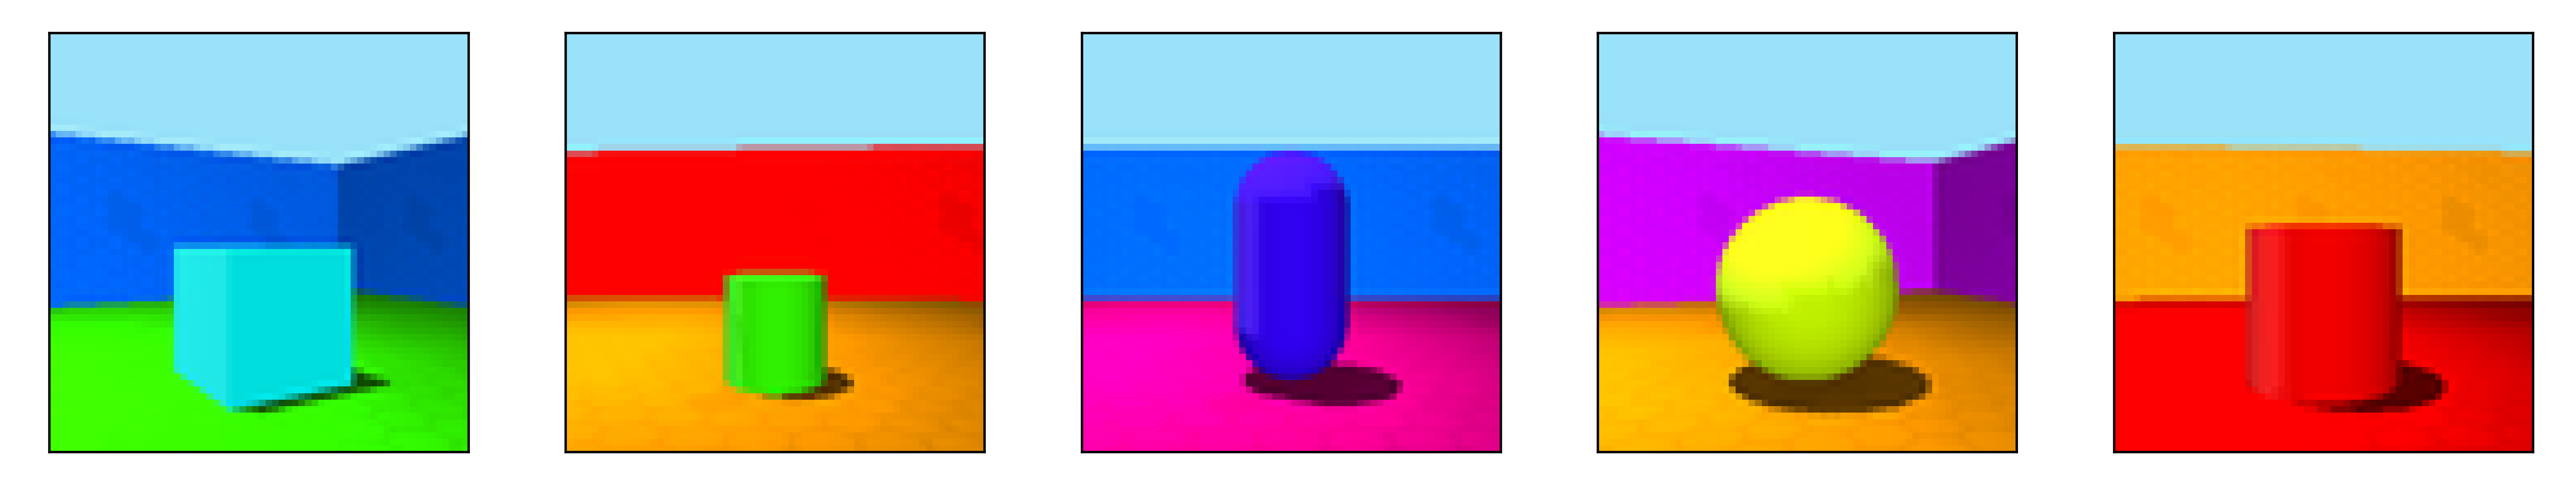
\includegraphics[width=\linewidth]{images/3dshapes_example.png}
\caption{Example images from the 3Dshapes dataset. Examples of corresponding generated exhaustive captions (from left to right): ``A big cyan block in the right corner on green floor in front of a medium blue wall.''; ``The green cylinder in the middle in front of a red wall on orange floor is tiny.''; ``A middle-sized dark blue pill located in the middle in front of a medium blue wall on pink floor.''; ``The picture shows a huge yellow ball on orange floor in front of a purple wall close to the right side.''; ``The large cylinder on red floor in front of a orange wall in the middle is red.''.}
\label{fig:3dshapes_example}
\end{figure}  

\subsubsection{Caption Generation}

The dataset provides symbolic feature labels of the images. However, since the goal of presented work is training artificial agents to use natural language in communication, English captions were generated for this dataset. More specifically, two annotations datasets were generated. 

The first dataset is tailored towards studying the effect of including maximally exhaustive image descriptions in the training data. Therefore, generated captions include natural language descriptions of all six features and their values, appearing in different syntactic constructions. All possible feature descriptions are listed in Table~\ref{tab:shapes_vocab}. Figure~\ref{fig:3dshapes_example} shows example images along with sample generated exhaustive captions. The syntactic variations were introduced in order to avoid potential effects of order in which descriptions of certain features might occur.
The captions were generated by constructing generation rules and sampling all possible resulting sentences using the \texttt{nltk} package \parencite{bird2006nltk}. The resulting dataset contains 20 synonymous captions per image, five of which are sampled at random for training in order to match the MS COCO conditions. The captions were build using a vocabulary of 49 tokens. Maximal caption length is 25 tokens, the minimal length is 16 and mean caption length is 18.9 tokens. 

The second dataset provides the comparison for investigating the role of having exhaustive captions compared to including shorter, less comprehensive captions, on the same dataset (\textbf{H8}). Additionally, this dataset with shorter captions is intended for investigating whether the models can learn to avoid overgenerating in their messages, while remaining informative.
That is, the exhaustivity manipulation is done on the same visual input, while keeping constant the vocabulary size. This dataset contains \textit{non-}exhaustive captions which only mention two to three out of six features of each image. These captions were generated using the same procedure. 27 captions per image were generated. The maximal caption length in this dataset is 13 tokens, the minimal is three tokens and the average length is 7.2 tokens.
The same examples along with non-exhaustive captions can be seen in Fig.~\ref{fig:3dshapes_example_short}.
The comparability of the vocabulary sizes is important in that it determines the difficulty of learning the policy for a given action space (which \emph{is} the vocabulary in case of communication) with REINFORCE which represents the functional learning in these experiments \parencite[cf.][]{havrylov2017emergence}.

The generation rules and the corresponding code can be accessed under \url{https://github.com/polina-tsvilodub/3dshapes-language}.

\begin{figure}
	\centering
	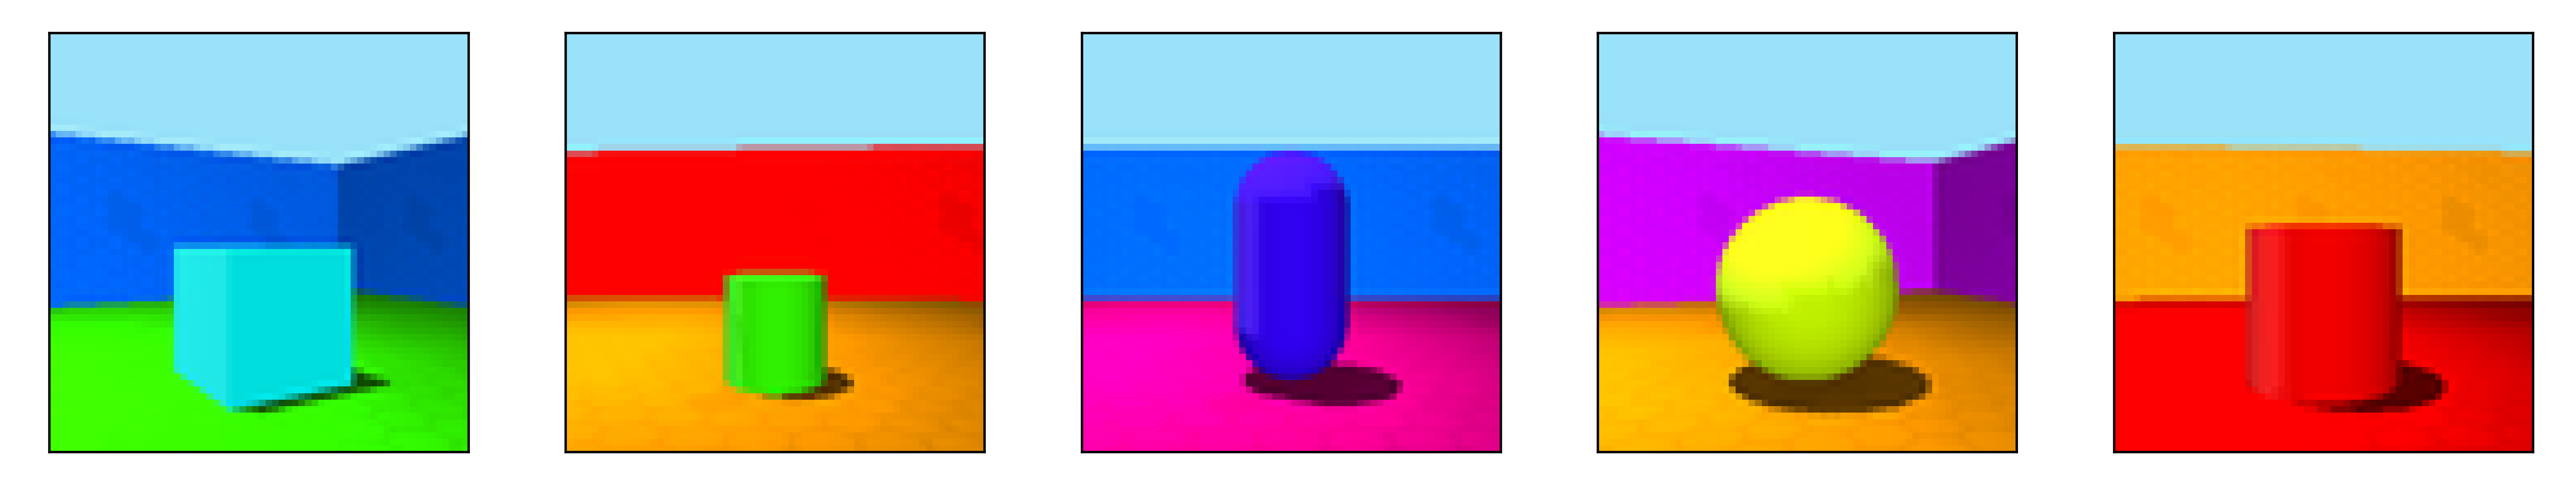
\includegraphics[width=\linewidth]{images/3dshapes_example.png}
	\caption{Example images from the 3Dshapes dataset. Examples of corresponding generated non-exhaustive captions (from left to right): ``The block is in front of a medium blue wall.''; ``A tiny cylinder.''; ``There is a pill in the middle.''; ``A yellow ball close to the right side.''; ``A red cylinder in front of a orange wall.''.}
	\label{fig:3dshapes_example_short}
\end{figure} 

Akin to MS COCO experiments, baseline experiments were conducted on random target-distractor pairs (an example pair can be found in Fig.~\ref{fig:shapes_randPairs_speaker_generations}). For the similar pairs experiments addressing \textbf{H5}, the distractor was chosen so that it matched the target with respect to at least three out of six features (see Fig.~\ref{fig:shapes_similarPairs_example_generations}).%For instance, if the target depicted a tiny red cube in the left corner on yellow floor and with blue background, the distractor could depict a tiny blue cube in the right corner on yellow floor and with green background.

%This dataset was chosen due to the systematicity of its content , allowing to generate natural language captions for each image which would exhaustively describe all features of the images. Since no such captions exist to the author's knowldege, they are generated as part of this thesis. To this end, a base context-free grammar (CFG) containing production rules for captions was manually created. The syntactic rules were constructed on the basis of examples of captions created by the author for samples from the dataset. Each caption must contain descriptions of all six feature dimensions. The terminal production rules mapping the pre-terminal to natural language labels are chosen for each image based on its unique feature value configuration. For each image, \pt{X captions are sampled from all the possible productions allowed by the grammar}.


\section{Architecture}
\label{architecture}
The architecture of the agents follows \textcite{lazaridou2020multi}, except for minor details to be explained below. As described in Chapter \ref{chapter03}, \textcite{lazaridou2020multi} explore different ways to parametrize the speaker agent, and the current work replicates the ``multi-task learning'' parametrization (p.~5). This choice is motivated by the fact that among their architectures, this is the only one where the speaker agent learns to produce messages and its core image captioning capability while having access to both the target and the distractor, as opposed to models relying on sampling captions from a pretrained single-image captioning models. The chosen architecture is used in all experiments. The model is visualized in Figure \ref{fig:architecture}.
\begin{figure}[h]
	\centering
	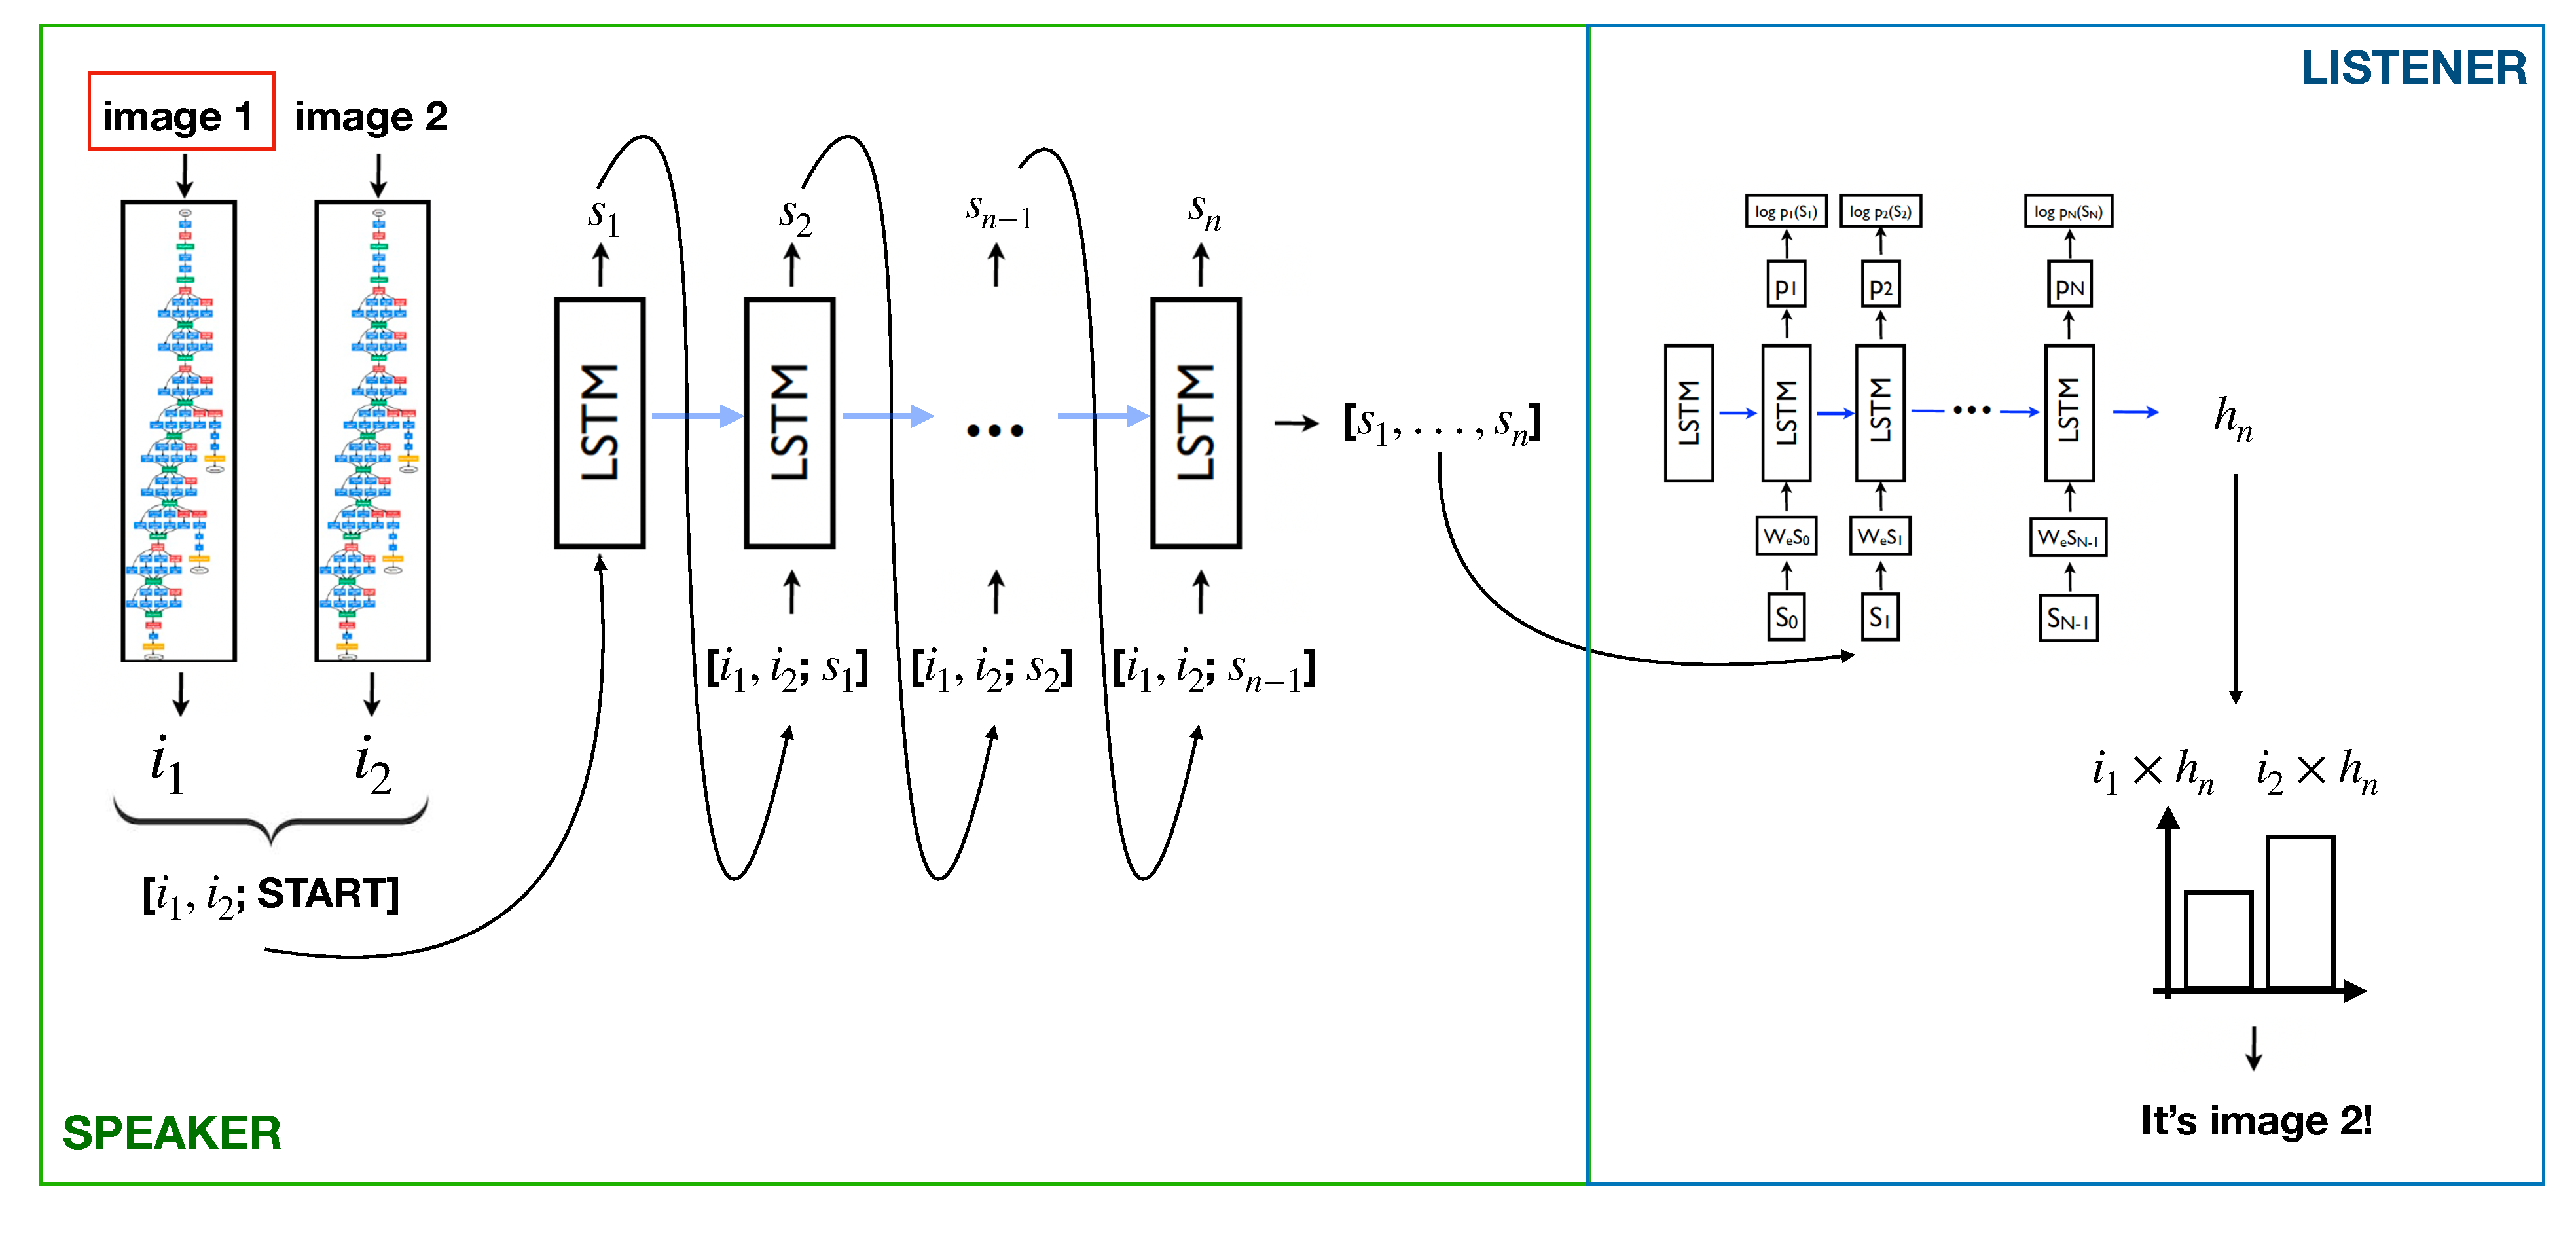
\includegraphics[width=\linewidth]{images/architecture_viz_cropped.pdf}
	\caption{Reference game architecture. The red box indicates the target referent (image 1). The LSTMs are presented unrolled in time. The image vector representations $i_1, i_2$ of the listener are extracted with an identical ResNet visual module as depicted for the speaker. Parts of Fig.~2 from \cite{vinyals2015show}, p.~3, were used for creating the diagram.}
	\label{fig:architecture}
\end{figure}  

Both agents have two components: a visual embedding module which takes as input the target and distractor images, and a language module. More specifically, the visual module for both agents embeds image features which were extracted using the same pre-trained ResNet50 model \parencite{he2016deep}. The weights were accessed through the \texttt{torchvision.models} API \parencite{marcel2010torchvision}. Features from all training images of the dataset were extracted and saved and then retrieved when training all agents. 
The language module differs for the two agents, so details are provided below. 
The code for all experiments and analyses can be found under \url{https://github.com/polina-tsvilodub/mSc-thesis}. 

\subsection{Speaker}
The speaker receives as input tuples \texttt{(targets, distractors)}, where \texttt{targets} as well as \texttt{distractors} are features for the sampled pairs extracted from the ResNet50, respectively. That is, the speaker knows which of the the two images in a given iteration of the reference game is the target for which the message should be produced. The speaker then produces a probability distribution over vocabulary tokens of the message given the input $P(m \mid i_t, i_d)$, parametrized by the speaker model parameters $\theta_S$. From a reinforcement learning perspective, training the speaker amounts to estimating the parametrized speaker policy $\pi_{\theta_s}(m \mid i_t, i_d)$.

The speaker model consists of a linear layer which projects the 2048-dimensional image features to 512-dimensional embedding space. The linear layer is applied to both the target and the distractor images, resulting in embeddings $i_t$ and $i_d$, respectively. The vectors are concatenated to $[i_t; i_d]$, the target embeddings always being the first ones, such that the speaker network implicitly knows which features represent the target. These 1024-dimensional vectors are used as additional context in the speaker's language module. The core of the module is the recurrent Long Short-Term Memory (LSTM) cell \parencite{hochreiter1997long}. More specifically, the language module consists of three layers: an embedding layer, mapping the vocabulary to 512-dimensional word embeddings, a one-layer LSTM with 512-dimensional hidden and cell states; and a linear layer on top, mapping the last hidden state of the LSTM to a distribution over the vocabulary. The size of the vocabulary depends on the dataset (see above).

During the reference game training, the speaker receives pairs of images, embeds them and prepends the concatenated embedding to the special \texttt{START} token. This 1536-dimensional embedding is then passed through the LSTM and the linear output layer. The next token is sampled from a categorical distribution parametrized with the probabilities computed from the hidden state in the previous timestep. The sampled token is concatenated with the image embeddings and input to the next timestep. This procedure repeats until the \texttt{END} token is sampled or the maximum caption length is achieved. All main experiments use the pure decoding strategy described above; yet some additional experiments investigate the effects of using greedy decoding (Section~\ref{expt:coco_greedy}). This architecture is also a common practice in image captioning literature (cf. Chapter \ref{chapter02}). Another possible approach that could be explored in future work would be to initialize the hidden states of the LSTM with the visual embeddings. In this case, the hidden and cell states of the LSTM were initialized with random values sampled from the standard normal distribution. The embedding and last linear layers' weights were initialized with random values sampled from the uniform distribution between -0.1 and 0.1, the biases were initialized with zeroes.  
This architecure results in a total of 9,402,838 trainable parameters (for a vocabulary  size of 4054) or a total of 5,297,713 parameters (for a vocabulary of 49 tokens) for both the visual and language module.  %\pt{Make a graphic of the models and / or the reference game}.

\subsection{Listener}
The listener receives as input the tuples \texttt{(images1, images2, messages)}, the first two inputs being ResNet50 features of the image pairs, input in random order, such that the agent doesn't know which image is the target. The \texttt{message} is the caption produced by the speaker. The listener then produces scores $P(i|m)$ over images identifying which one is the target, parametrized by the listener model parameters $\theta_L$.

The message is passed to the language module which consists of an embedding layer, mapping the vocabulary to 512-dimensional word embeddings, and a one-layer LSTM with 512-dimensional hidden and cell states. All weights are initialized analogously to the respective weights of the speaker model. The hidden cell state $h_n$ at the last time step of embedding the received message is used as the final message representation. 
The visual module of the listener consists of a linear layer which also projects the 2048-dimensional image features to a 512-dimensional embedding space. The images are passed through the linear layer one after the other, resulting in embeddings $i_1$ and $i_2$. Finally, the listener computes dot products between each image embedding and the message embedding. The dot products are used to parametrize a categorical distribution over the image indices; the target is then sampled from this distribution.  
The architecture results in 1,049,088 trainable parameters for the listener's visual module and 4,176,896 (for 4054 tokens) trainable parameters for its LSTM (2,126,336 parameters for 49 tokens).


\subsection{General Training Details}
\label{general_train_details}
All experiments were trained with a batch size of 64 pairs, using the Adam optimizer with a learning rate  of 0.001 \parencite{kingma2014adam}. In the reference game setting, due to computational constraints, the models were trained for two epochs per experiment. \footnote{Pretraining and some experiments were conducted on a MacBook Pro with four Intel cores i7-1068NG7 with CPU @ 2.30GHz. On average, pretraining took 2h/epoch, reference games took 6h/epoch. Remaining experiments were conducted using Google Colab and their Tesla P100 GPU with 16GB memory. There, reference game training took on average 3h/epoch.} 

In the reference games, following \cite{lazaridou2020multi}, the speaker parameters $\theta_S$ were updated by optimizing a compound loss function $J_s$. More precisely, the speaker loss consisted of a weighted sum of a functional loss $L_f$ and a structural loss $L_s$. The former was computed via the REINFORCE rule based on the listener's task performance (i.e., referential success, providing the functional learning signal necessary for investigating especially \textbf{H1--H3}). The speaker received the reward $r$ 1 if the listener guessed the target successfully, and -1 otherwise. The structural loss was a supervised training loss, computed via cross-entropy between the message produced by the speaker and the ground truth caption for the given target image. $L_f$ additionally included an entropy regularization term, weighted by 0.1. That is, the single loss components were \parencite[following][]{lazaridou2020multi}\footnote{The only difference was the extension of the conditioning to both $i_t, i_d$ instead of $i_t$ only in \cite{lazaridou2020multi}.}:
\begin{dmath}
L_f = -r \;\sum_{m=0}^{t}\; log \; P_{\theta_S}(caption^m|caption^{<m}, [i_t, i_d]) - 0.1 \; (- \sum_{m=0}^{t} P_{\theta_S}(caption^m|caption^{<m}, [i_t, i_d]) \; log \; P_{\theta_S}(caption^m|caption^{<m}, [i_t, i_d])) \\
{L_s = \sum_{m=0}^{t}log \; P_{\theta_S}(caption^m|caption^{<m}, [i_t, i_d])}
\end{dmath}
where $i_t, i_d$ were the image vectors, $t$ was the length of the message, $caption^{<m}$ was the message up until the $m$-th token ($m \leq t$) and $P_{\theta_S}$ was initialized with the pretrained speaker. The resulting total loss was:
\begin{equation}
J_s = (1-\lambda_s)L_f + \lambda_s L_s
\end{equation}
In particular, the structural loss weight $\lambda_s$ was varied in some experiments in order to address \textbf{H4}.
The listener parameters $\theta_L$ were updated via cross-entropy loss $J_L$ optimized based on the guessed target index compared to the ground truth target. 

\subsubsection{Hypotheses Operationalization}
Given the experimental architecture reported above, this section describes more specific operationalizations of the hypotheses about language drift which may occur in the experiments, presented in Section \ref{hypos}.\\
\newline
\textbf{H1}--\textbf{H2}, \textbf{H6}--\textbf{H8} concern structural and semantic drifts, relative to functional improvement of the agents (i.e., the speaker's functional loss improvement and listener's task accuracy increase). The former is operationalized as decreasing log probability of the speaker's message under a pretrained LM. The latter is operationalized as decreasing conditional log probability of the speaker's message given the target image, under the pretrained speaker model. \newline
\textbf{H3:} The overlap metrics are expected to increase with functional improvement of the agents. Furthermore, since they should capture functional adequacy of the speaker's messages, they are expected to increase stronger as the functional learning signal in the reference games becomes stonger.\newline
\textbf{H4:} Given that the pressure to stay close to the natural language distribution is provided by the structural loss component $L_s$ in the models, it is expected that both the structural and the semantic drifts increase as the weight of the structural loss component $\lambda_s$ decreases. To investigate this, five reference games with the structural loss weights $\lambda_s \in \{0, 0.25, 0.5, 0.75, 1\}$ were conducted. The functional loss component was computed as $\lambda_f = 1 - \lambda_s$, respectively. That is, the drifts are expected to increase as $\lambda_s$ approaches 0.\newline
\textbf{H5:} The discriminativity of the captions is expected to increase less in the similar target-distractor pairs experiment than in the baseline experiment on random pairs. That is, the difference to the pretrained speaker in terms of overlap values is expected to be smaller than in the random pairs experiments due to the higher perceptual and referential difficulty of discriminating images depicting similar things. 

\section{Experiment Procedures and Results}

This section first provides an overview of speaker pretraining, before zooming in on conducted experiments and discussing their procedures as well as results with respect to the described hypotheses.
First, a general pipeline of the main reference games as it applies to all experiments described below is provided.

\subsubsection{General Procedure}
\begin{enumerate}
	\item Speaker and potentially listener models are instantiated with pretrained weights. The experiment is configured with parameters like the decoding strategy, listener type, structural loss weight etc. (see experiments below for details).   
	\item Training image pairs are created from a set of 30,000 images and all five captions for each image unseen during pretraining, resulting in (approximately) 150,000 training pairs, batched into batches of 64 pairs. This results in 2343 training steps per epoch. The pairs are constructed either at random (while making sure the two images are not the same) or by choosing similar target-distractor pairs. 
	\item During each step, the agents play one reference game round: the speaker sees a target in context of a distractor and generates a messages about the target which is received by the listener. The listener sees the same images and picks the target based on the speaker's message. The speaker is updated according to both the structural well-formedness of her message compared to the ground truth caption of the target and the listener's success; the listener is updated according to its task success. 
	\item Each 200 steps of training, the structural and semantic drift metrics are computed on three held out batches (192 images) in order to observe their dynamics.
	\item After training, the agents are evaluated on a held out test set of 1,000 images which were neither part of pretraining nor reference game training. During the evaluation, the agents are put in evaluation mode and the listener accuracy and all the drift metrics are computed. If the agents were trained on random image pairs, the 1,000 images are grouped into random pairs, if on similar image pairs---into similar pairs, respectively. These are the pairs the reported test accuracies are computed on. Generally, the drift values of the ground truth captions of the test sets and of the respective pretrained speaker captions on the test sets are treated as benchmarks for comparing drift dynamics.
\end{enumerate}
Specific configurations of each experiment are described in the respective sections. 

\subsection{Speaker Pretraining}
\label{speaker_pretraining}
\begin{figure}[h]
	\centering
	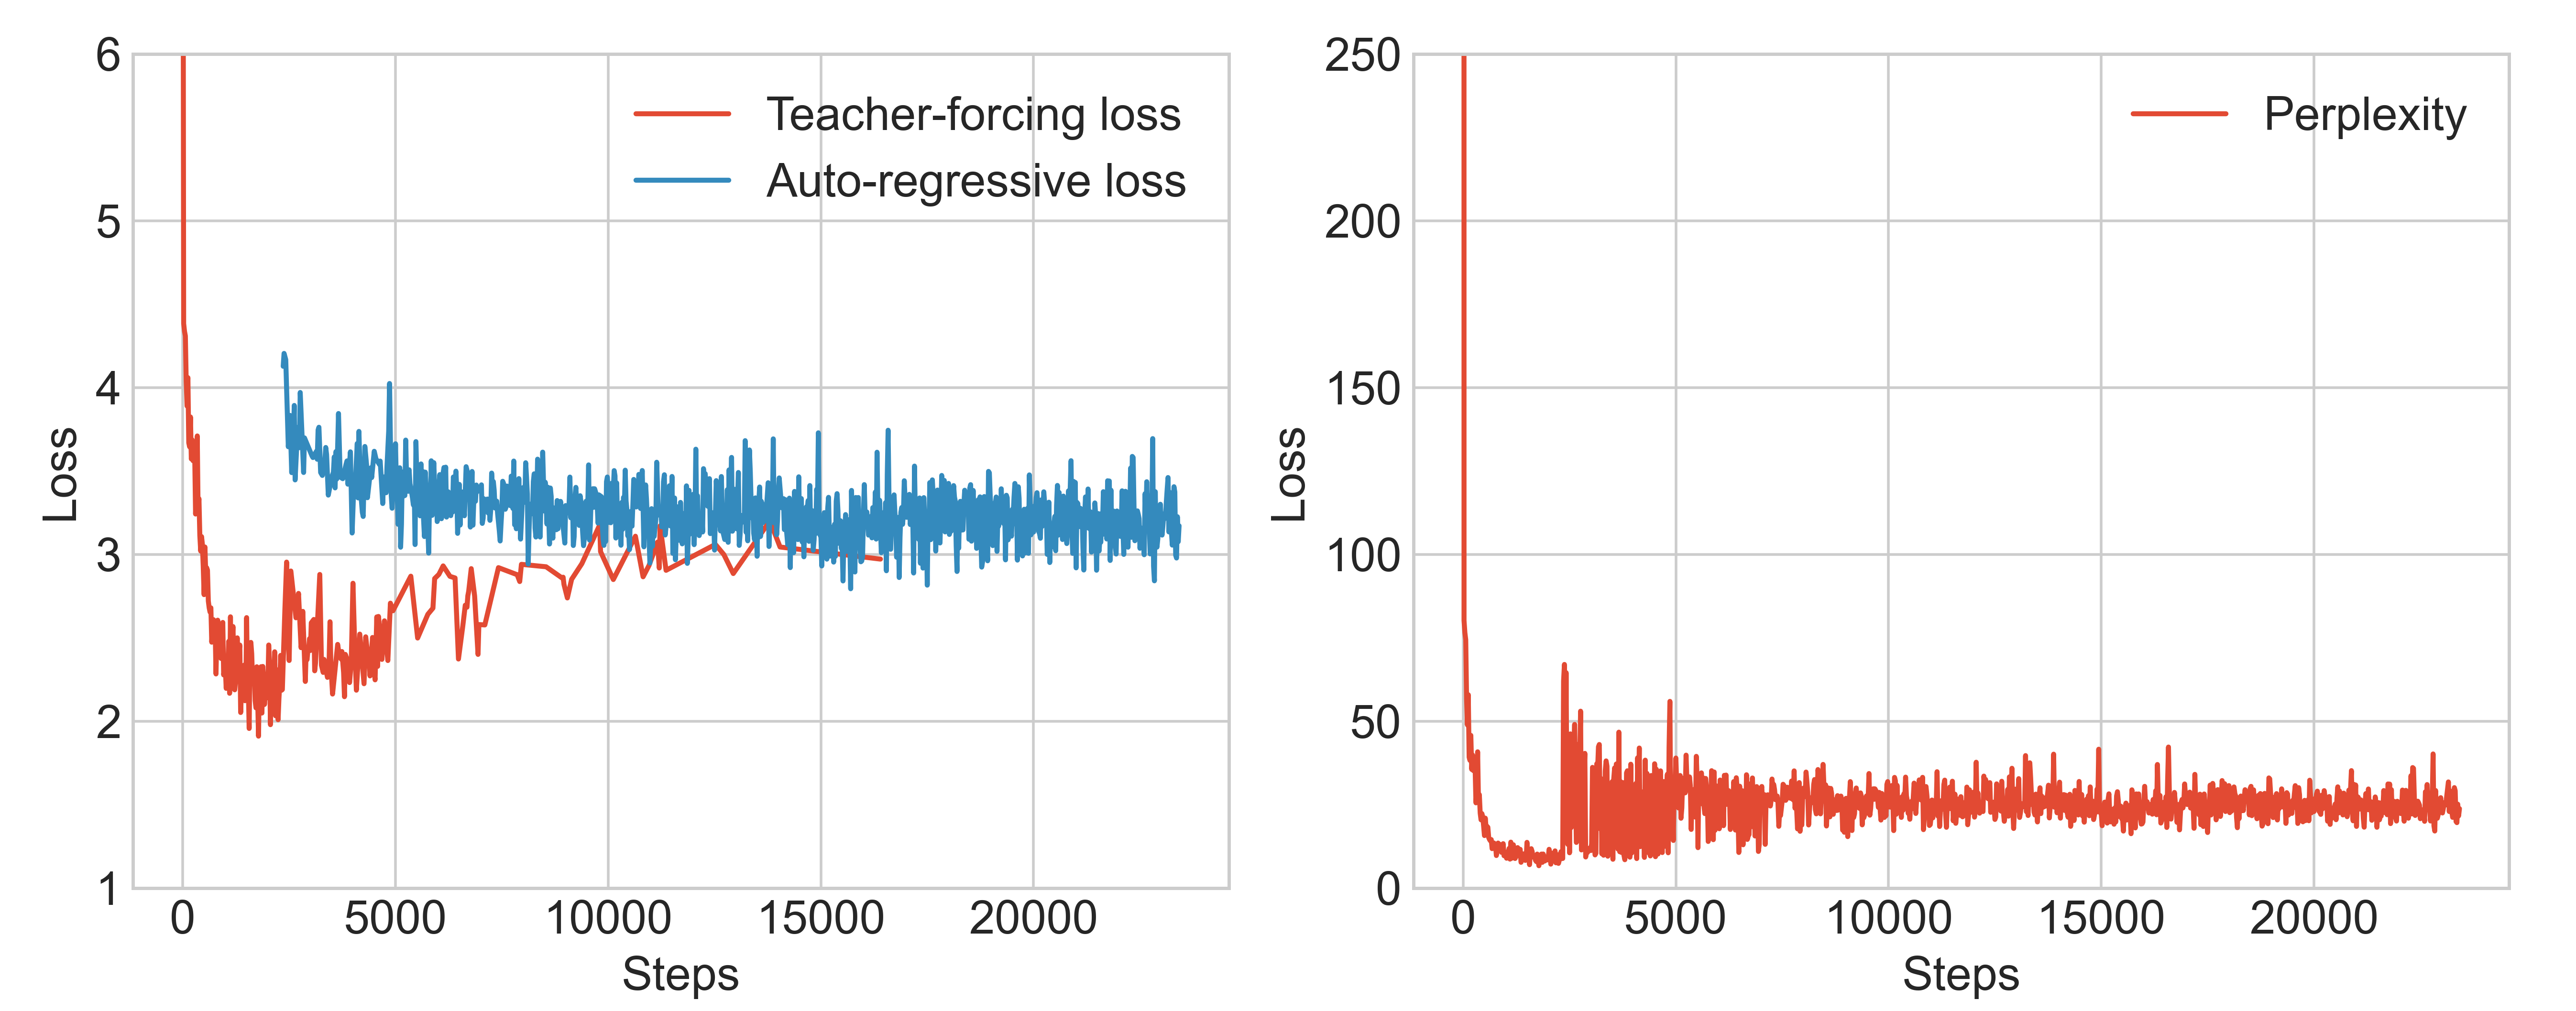
\includegraphics[width=\linewidth]{images/coco_pretraining_losses_ppls.png}
	\caption{Left: Training losses during pretraining the speaker on MS COCO; the colors indicate the pretraining mode, i.e., whether the ground truth caption (teacher-forcing loss, red) or the self-generated token (auto-regressive loss, blue) from the previous timestep was supplied at each timestep. Right: Training perplexity during pretraining of the speaker on MS COCO.}
	\label{fig:coco_pretraining}
\end{figure}  

\begin{figure}[h]
	\centering
	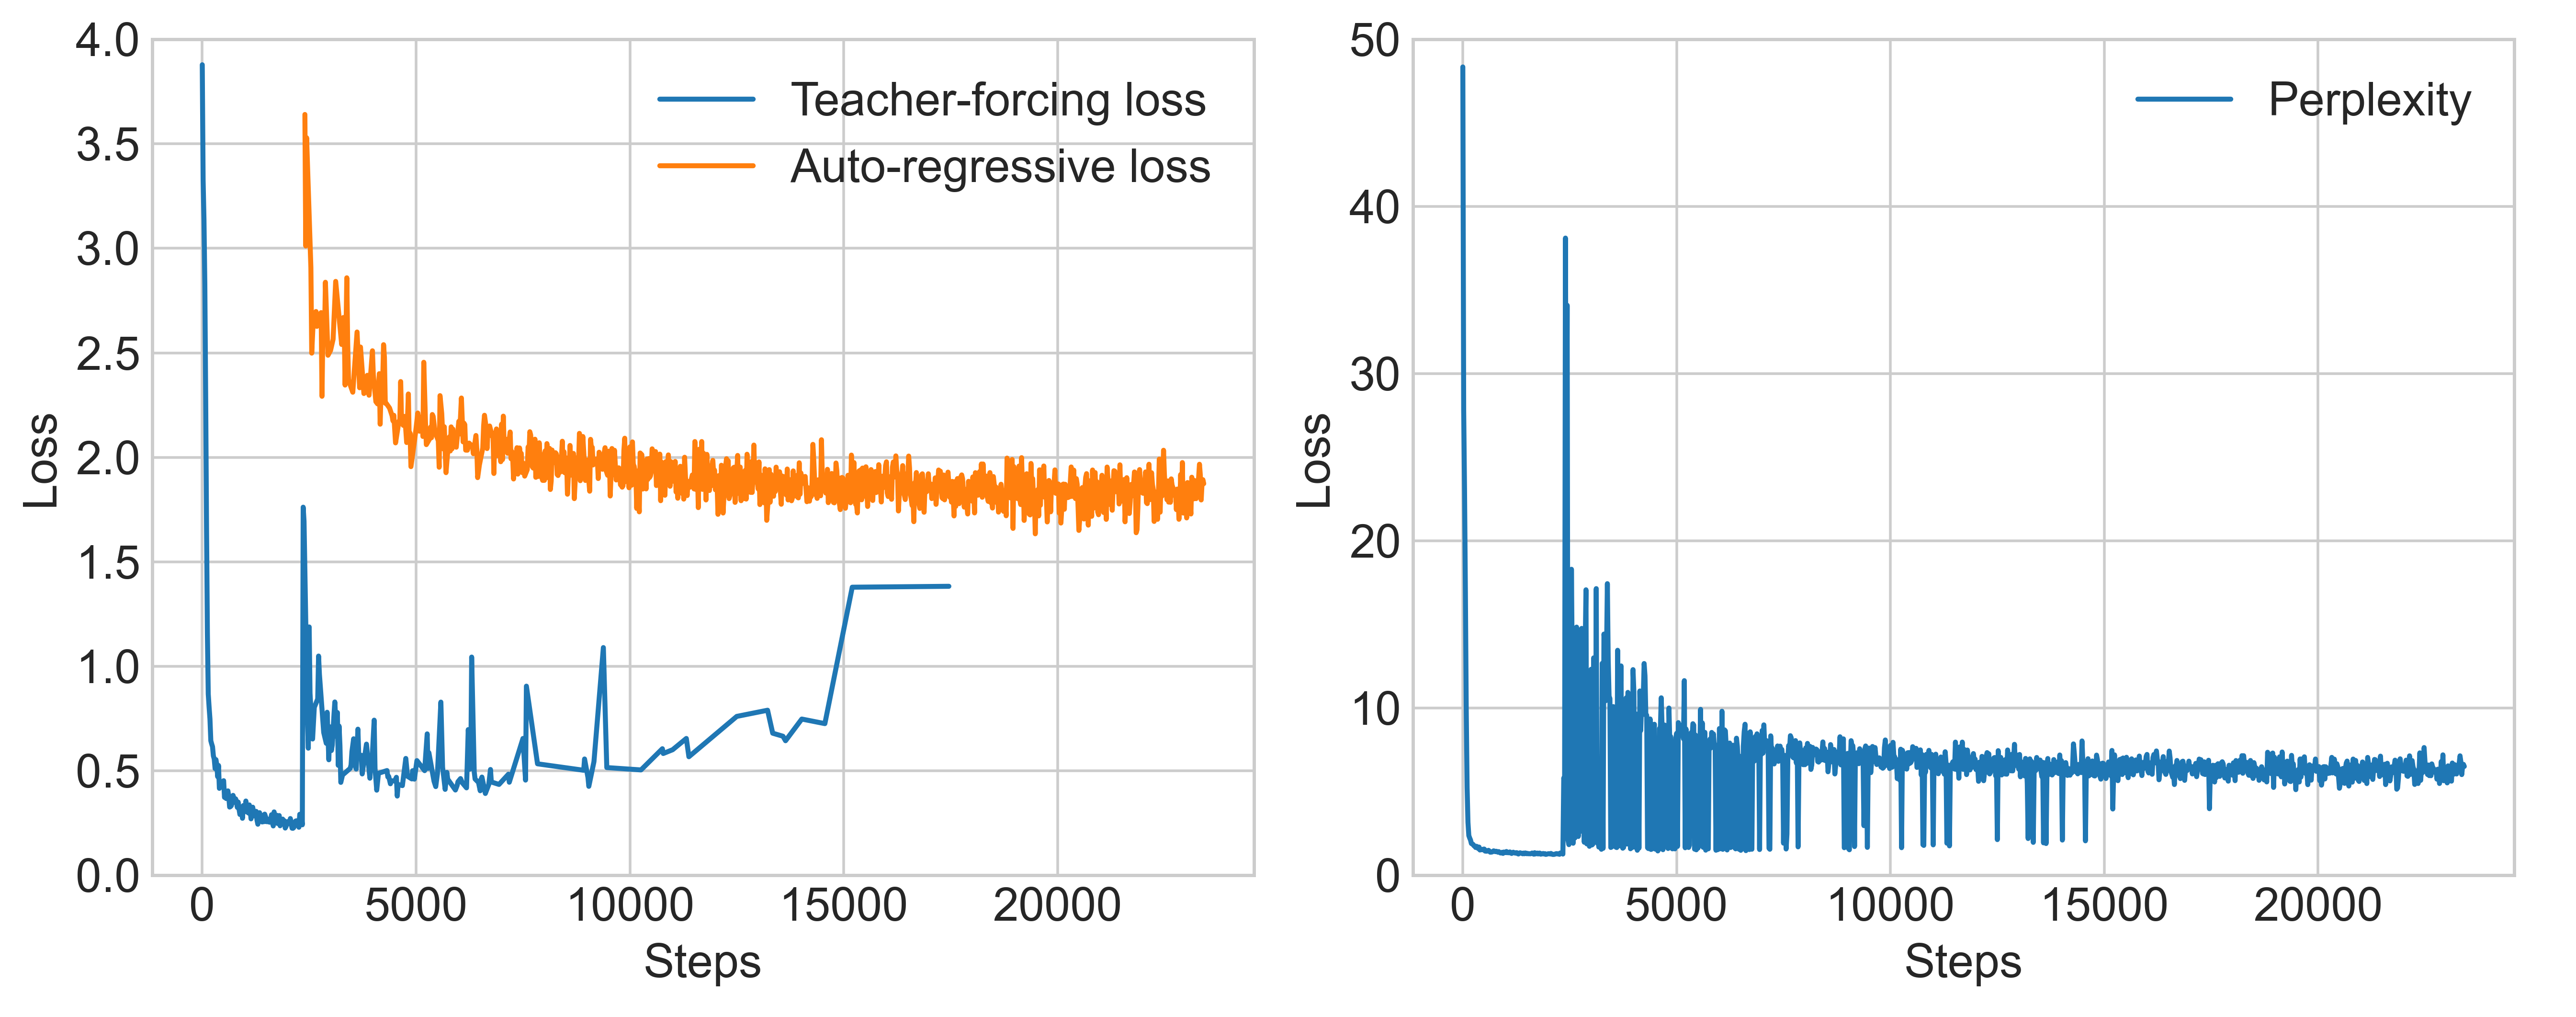
\includegraphics[width=\linewidth]{images/3dshapes_pretraining_losses_ppls.png}
	\caption{Left: Training losses during pretraining the speaker on the exhaustive 3Dshapes dataset; the colors indicate the pretraining mode, i.e., whether the ground truth caption (teacher-forcing loss, blue) or the self-generated token (auto-regressive loss, orange) from the previous timestep was supplied at each timestep. Right: Training perplexity during pretraining of the speaker on 3Dshapes.}
	\label{fig:3dshapes_pretraining}
\end{figure}  

\begin{figure}[h]
	\centering
	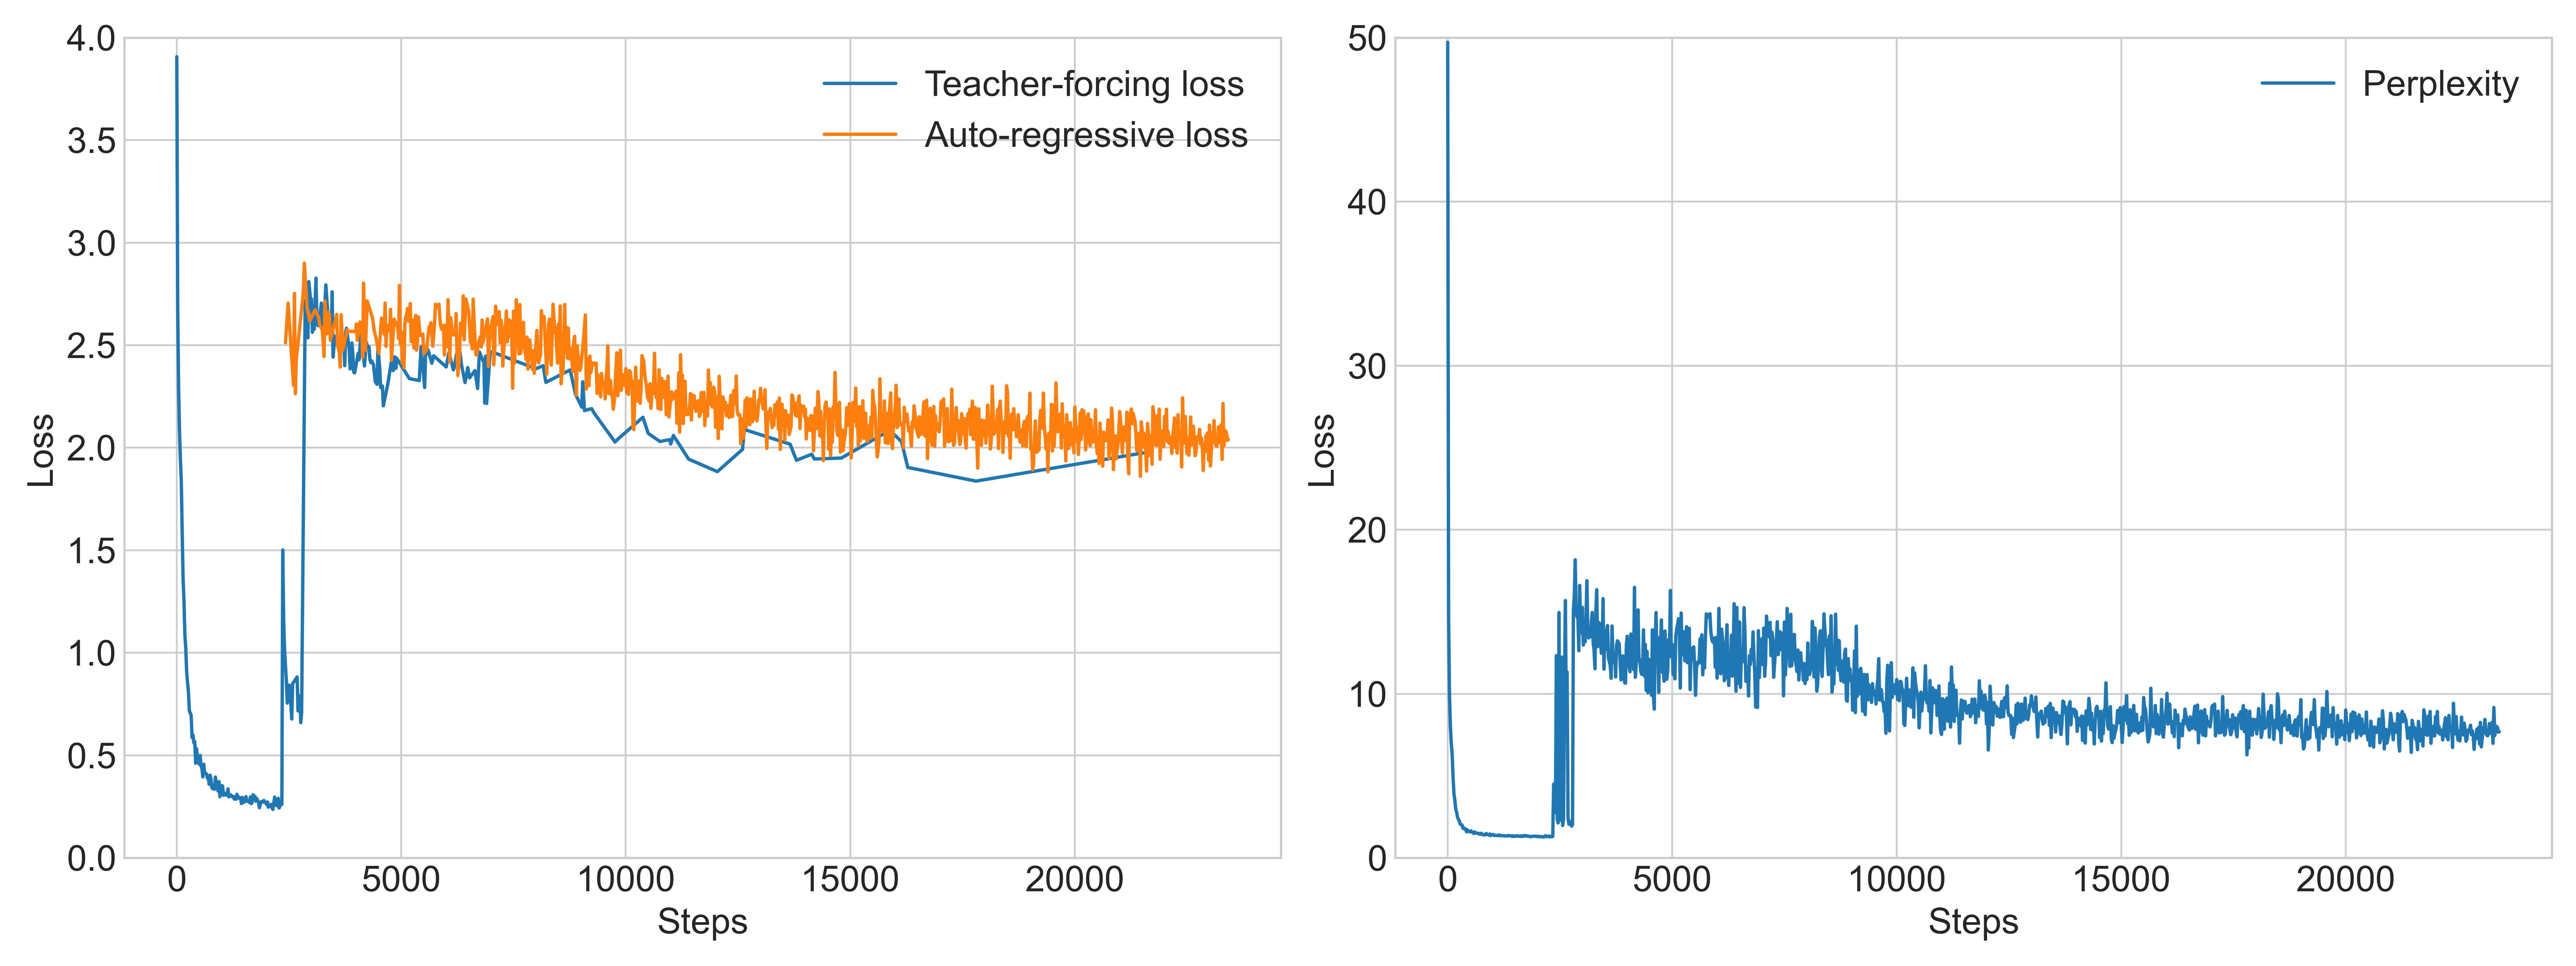
\includegraphics[width=\linewidth]{images/3dshapes_wShort_pretraining_losses_ppls.png}
	\caption{Left: Training losses during pretraining the speaker on the 3Dshapes dataset which includes both short and exhaustive captions; the colors indicate the pretraining mode, i.e., whether the ground truth caption (teacher-forcing loss, blue) or the self-generated token (auto-regressive loss, orange) from the previous timestep was supplied at each timestep. Right: Training perplexity during pretraining of the speaker on 3Dshapes.}
	\label{fig:3dshapes_pretraining_wShort}
\end{figure}  
%Table with image caption quality metrics of the pretrained speakers. Add same metrics of the speaker agents after ref games as rows to the same table. 

\begin{table}[]
	\begin{tabularx}{\textwidth}{|X|l|l|l|l|l|l|l|}
		\hline
		\textbf{Model name}                                    & \textbf{B-1} & \textbf{B-2} & \textbf{B-3} & \textbf{B-4} & \textbf{M} & \textbf{C} & \textbf{Val. loss} \\ \hline
		Pretrained MS speaker                             & 0.408           & 0.137           & 0.042           & 0.013           & 0.116           & 0.165          & 4.079                    \\ \hline
		%MS Baseline, random, $\lambda_s = 0$      &   0.405              &      0.130           &     0.036            &     0.009            &     0.116            &     0.177           &           4.124               \\ \hline
		%MS Baseline, random, $\lambda_s = 0.25$   &          0.413       &       0.134          &      0.041          &       0.015          &       0.116          &       0.189        &           4.074               \\ \hline
	%	MS Baseline, random, $\lambda_s = 0.5$   &          0.397       &       0.124          &      0.036          &       0.012          &       0.115          &       0.170         &           4.082               \\ \hline
		MS Baseline, $\lambda_s = 0.75$   & 0.407           & 0.133           & 0.037           & 0.010           & 0.116           & 0.178          & 4.056                    \\ \hline
	%	MS Baseline, random, $\lambda_s = 1$   &    0.405             &   0.125              &    0.033             &  0.000              &         0.115        &       0.181         &         4.066                 \\ \hline
	%	MS Baseline, random, similar pairs, $\lambda_s = 0.75$   &    0.292           &   0.066              &    0.010           &  0.000              &         0.068       &       0.018        &         4.180        \\ \hline
	%	MS Baseline, similar, random pairs  &     0.396            &          0.123       &       0.031         &        0.000         &   0.113         &      0.115          &      4.078                   \\ \hline
		MS similar  &     0.222    &          0.055       &       0.015         &        0.000         &   0.074              &      0.232         &      4.235                    \\ \hline
		MS fixed listener, random, $\lambda_s = 0.75$  &        0.393         &       0.132          &        0.040         &      0.011           &      0.113           &        0.177        &       4.117                   \\ \hline
		Pretrained 3D speaker exh.    & 0.671           & 0.343           & 0.163           & 0.077           & 0.283           & 1.026          & 2.091                    \\ \hline
		Pretrained 3D speaker mixed    &  0.307          &  0.111  &  0.039     & 0.014       &  0.145   &    0.112 &    2.784      \\ \hline
		3D Baseline, $\lambda_s = 0.75$  & 0.672           & 0.340           & 0.159           & 0.074           & 0.284           & 1.068          & 2.089                    \\ \hline
		3D similar, $\lambda_s = 0.75$ & 0.673           & 0.335           & 0.152           & 0.070           & 0.279           & 1.033          & 2.103                    \\ \hline
		3D Baseline, fixed listener, $\lambda_s = 0.75$ &      0.684           &   0.353      &    0.172       &     0.084   &      0.288   &     1.137  &     2.068        \\ \hline
	\end{tabularx}
\caption{\label{tab:eval_metrics_refgame}Caption evaluation metrics and the validation loss on a heldout dataset, computed for the initial pretrained speakers and speakers after training on representative reference games on both datasets. \textbf{B} denotes BLEU, \textbf{M} the METEOR score, \textbf{C} the CIDEr score, ``MS'' the MS COCO dataset and ``3D'' the 3Dshapes dataset. ``Baseline'' refers to the setup wherein the listener is trained jointly with the speaker, using pure decoding. ``Random'' refers to speakers trained on random target-distractor pairs; ``similar'' refers to speakers trained on similar target-distractor pairs.}
\end{table}

Before conducting reference games, the speaker agents were pretrained for both the MS COCO and 3Dshapes experiments. Conceptually, the model was pretrained in order to learn the statistical properties of English, i.e., ``learn to speak'', before being fine-tuned on the functional reference game task. This can be motivated as providing general \textit{task-unconditional} linguistic capabilities to the speaker which she can then transfer to specific tasks.

Both speakers were pretrained in a supervised fashion by sampling tuples of the form $(i_t, i_d, c_t)$ where $i_t, i_d$ were the target and distractor images, and $c_t$ was the target ground truth caption. The models were pretrained on 30,000 images selected at random from the respective dataset; for each image, the model saw five available ground truth captions. 
The pretraining was accomplished with the cross-entropy loss. Models for both datasets were trained for ten epochs.

As described in Section \ref{model_pretraining}, there are different strategies for pretraining the speaker. Based on initial exploratory experiments reported in Appendix \ref{app:grid_search}, all speakers were pretrained using a decreasing teacher-forcing rate $0.5^{epoch-1}$, transitioning to auto-regressive training with pure decoding. That is, in the auto-regressive mode the model was fed its own predicted token from the previous timestep during training; that token was generated by pure sampling. In teacher-forcing rounds, the ground truth tokens were fed instead. For monitoring the pretraining, both the loss dynamics and the perplexity (PPL) were used; perplexity is a computed as $exp(H(m))$ where $H(m)$ is the cross-entropy measure of a produced caption $m$, and presents a common evaluation metric for language models in NLP.
Speakers for both datasets were pretrained in this set up. Figure \ref{fig:coco_pretraining} shows the pretraining dynamics of the MS COCO speaker, Figure \ref{fig:3dshapes_pretraining} shows the dynamics of the 3Dshapes speaker pretrained on exhaustive captions. Additionally, another 3Dshapes speaker was pretrained on both exhaustive and short captions from the second 3Dshapes annotations dataset (\textit{mixed lengths} speaker). More precisely, for each image, five ground truth captions were selected, sampling at random whether three out of five captions were short or exhaustive. This additional speaker was trained for the experiments with short captions (addressing \textbf{H8}) in order to induce a bias towards actually generating short captions from pretraining; otherwise, without explicit pressure towards generating shorter messages, the speaker would be expected to produce exhaustive caption length messages \parencite[cf., e.g.,][]{hupkes2020compositionality}. The pretraining results can be seen in Figure \ref{fig:3dshapes_pretraining_wShort}.

The evaluation of their image captioning capabilities on standard metrics (introduced in Chapter \ref{chapter02}) after pretraining can be found in Table \ref{tab:eval_metrics_refgame}. The metrics were computed on a held out validation split with 5,000 unique images and respective captions. Comparing the pretrained speakers to state-of-the-art image captioning model peformance in Table \ref{tab_coco_metrics_ref} and inspecting example image captions (see Fig.~\ref{fig:coco_randPairs_speaker_generations}, pretrained speaker), it is apparent that the MS COCO speaker performed somewhat worse in terms of standard caption evaluation metrics. It is hypothesized that this is due to the mixed teacher-forcing and auto-regression pretraining modes. It is conjectured that the speaker quality might only affect the absolute performance and drift metric values, but the qualitative comparisons between experiments will remain unaffected because all experiments are based on the same pretrained speakers. The 3Dshapes exhaustive speaker showed quite competitive results in terms of absolute values, yet there are no benchmarks in the literature. The mixed lengths speaker was comparable to the MS COCO one. Example generations from the pretrained speakers, however, also indicate that the captions are not completely well-formed (see Fig.~\ref{fig:shapes_randPairs_speaker_generations}--\ref{fig:shapes_similarPairs_example_generations}).
Furthermore, all language drift metrics were computed for the pretrained models, presenting a baseline for linguistic capabilities, before any deterioration might take place due to task optimization (see Tables \ref{tab:coco_drift_metrics_basic}, \ref{tab:3dshapes_drift_metrics_basic_baseline}).

Equipped with the pretrained speaker agents, the reference game experiments are described below. First, main experiments on the MS COCO dataset are introduced. Then, the 3Dshapes experiments are presented. Note that the standard image captioning evaluations were performed on representative sample reference games in order to estimate their overall match with language drift metrics rather than gather comprehensive results. These sample experiments were the baseline, the basic similar pairs experiment and the baseline experiment with a fixed listener, on both datasets (details are provided in the following sections).

\subsection{MS COCO: Baseline Experiments}
\label{expt:coco_baseline}

\begin{table}[]
	\begin{tabularx}{\textwidth}{|X|l|l|X|X|X|}
		\hline
		\textbf{Model name}                                    & \textbf{log $P(m)$} & \textbf{log $P(m \mid i)$} & \textbf{Overlap (d)} & \textbf{Overlap (c)} & \textbf{Acc. } \\ \hline
		Ground truth val.               &     -108.566            &          -80.399             &    9.147           &       0.038          &  0.963 (fixed listener)                  \\ \hline
		Ground truth similar val.               &     -110.074        &       -79.991           &             &           &      ---         \\ \hline
		Pretrained MS speaker               &      -131.598            &           -62.385             &          1.194            &           0.003           & 0.902 (fixed listeners)                 \\ \hline
		MS Baseline, random, $\lambda_s = 0$      &     -131.890              &         -63.319               &        1.259       &         0.003             &             0.924                        \\ \hline
		MS Baseline, random, $\lambda_s = 0.25$    &      -133.954             &          -65.533              &          1.173            &       0.004               &           0.935               \\ \hline
		MS Baseline, random, $\lambda_s = 0.5$      &         -133.595         &           -67.904             &        1.106              &        0.001              &             0.890                 \\ \hline
		MS Baseline, random, $\lambda_s = 0.75$   &       -135.910            &             -71.819          &        1.197              &        0.000              & 0.953                \\ \hline
		MS Baseline, random, $\lambda_s =1$  &      -136.762             &          -70.454              &         1.125             &          0.001            &                   0.914         \\ \hline
		MS Baseline, similar, $\lambda_s = 0.75$  &     -133.093              &       -66.955                &               0.155       &       -0.001               &        0.648            \\ \hline
		MS, random, fixed listener, $\lambda_s = 0$  &         -130.624         &           -62.095             &     1.201                 &        0.003              &                          0.888               \\ \hline
		MS, random, fixed listener, $\lambda_s = 0.75$  &         -134.408          &           -67.627             &     1.042                 &        0.003              &                          0.881     \\ \hline
	\end{tabularx}
\caption{\label{tab:coco_drift_metrics_basic} Language drift metrics and listener test accuracies (``Acc'') on different image pairs. 
	``Baseline'' refers to joint speaker and listener training using pure decoding. MS refers to the MS COCO dataset. ``Random'' refers to speakers trained on random target-distractor pairs; ``similar'' refers to speakers trained on similar pairs. ``Overlap (d)'' refers to the discrete overlap metric, ``overlap (c)'' to continuous overlap.}
\end{table}

As described in the general procedure, the baseline experiment on MS COCO was conducted on 30,000 images which were not used during pretraining. The target-distractor pairs were constructed at random. Pure decoding was used for sampling the speaker's message, and the weight of the structural loss was $\lambda_s = 0.75$. The weight of the functional loss was $\lambda_f = 0.25$, respectively. These configurations are treated as the baseline experiment since preliminary explorations revealed that these are the minimal requirements for a successful reference game (see Appendix \ref{app:grid_search} for details). The training dynamics can be seen in Figure \ref{fig:coco_baseline_speaker_loss_listener_acc_all} (red lines). Example messages produced by the speaker can be found in Figure~\ref{fig:coco_randPairs_speaker_generations} (baseline speaker).

For computing the test task accuracy, listener accuracy was computed on a held out validation set of 1000 pairs of images which were neither part of pretraining nor the reference game training. The test performance was estimated by sampling captions from the speaker using pure decoding, like during training, although it is also common to use greedy decoding at inference time in NLP. The test accuracy of 0.953 in Table \ref{tab:coco_drift_metrics_basic} shows that the agents successfully learned to play the reference game. Furthermore, supporting \textbf{H1} and \textbf{H2}, the language underwent deterioration, both syntactically and semantically, compared to the pretrained speaker. More specifically, the average log probability of the generated captions under the pretrained Transformer XL model decreased by 4.312, compated to the log probability of captions generated by the pretrained speaker. Similarly, the conditional log probability of the generated captions given the target images decreased by 9.434, compared to the conditional probability of the captions from the pretrained speaker (Table \ref{tab:coco_drift_metrics_basic}, first two columns, ``Pretrained MS speaker'' vs. ``MS Baseline, random, $\lambda_s=0.75$''). The dynamics of structural and semantic drifts during training can be seen in Figure \ref{fig:coco_baseline_str_sem_drift_all} (red lines). To this end, following general procedure, the structural and semantic drift metrics were computed every 200 training steps on 192 held out image pairs (three batches).\footnote{The number of metric computation steps was restricted to only three batches due to computational constraints.} Due to the small size of the decrease as well as the small number of validation batches, no trend can be observed visually.
As for the other drift metrics presented in Table \ref{tab:coco_drift_metrics_basic} (third and fourth columns), only negligible differences to the pretrained speaker can be observed: a slight increase in the discrete overlap metric might suggest that the speaker learned to produce messages that are more appropriate for the target compared to the distractor, and, therefore, might be more discriminative. On the other hand, the similarity of embeddings of the ground truth caption and the message decreased relative to the distractor similarity, compared to the pretrained speaker. This might be due to the difficulty to propagate the learning signal all the way to the embedding layer. Furthermore, the comparison to the overlap values of the ground truth captions indicates that the difference in terms of used tokens between target and distractor captions is much more pronounced in the dataset than what is propagated by the trained model (Tab.~\ref{tab:coco_drift_metrics_basic}, first line, third and fourth columns).  
Therefore, to sum up, \textbf{H3} is not borne out in this experiment.

Additionally, the fine-tuned speaker was also evaluated with standard image captioning metrics. Table \ref{tab:eval_metrics_refgame} shows that caption quality marginally decreased with respect to almost all metrics, confirming the trend shown by the structural and semantic language drift metrics. 

\begin{figure}[h]
	\centering
	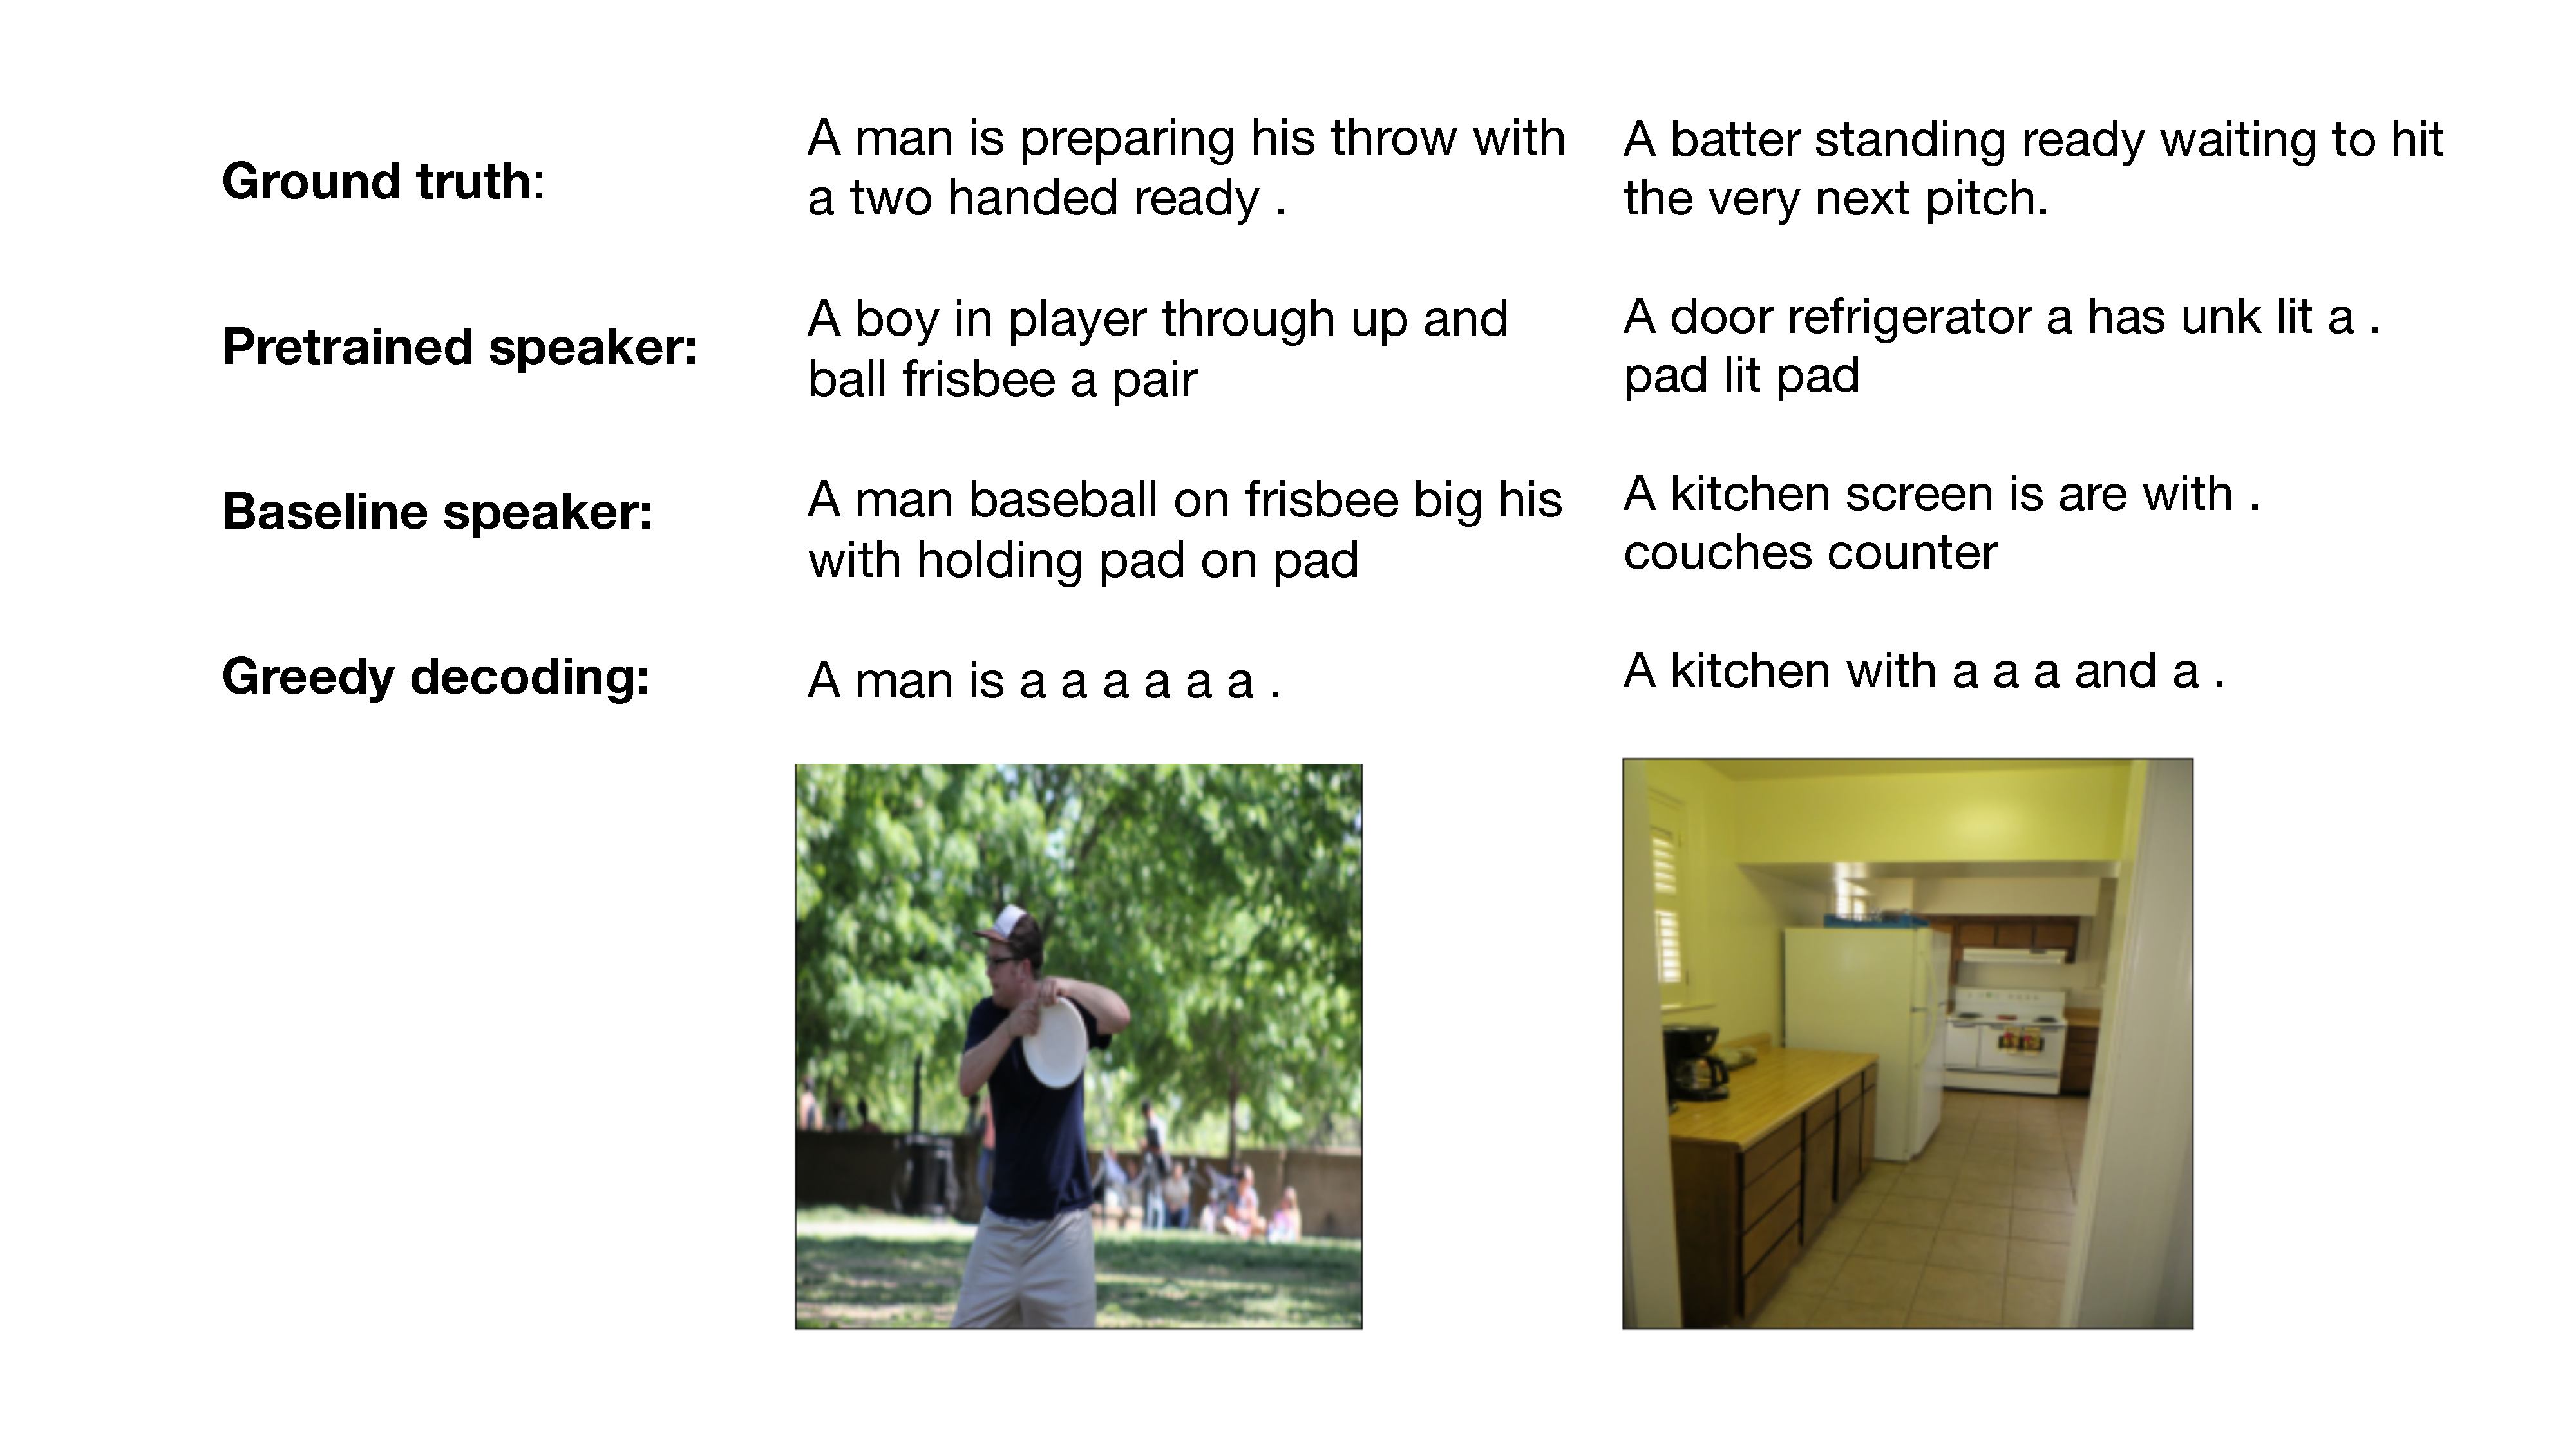
\includegraphics[width=\linewidth]{images/example_generations/coco_speakers_randomPairs_examples.pdf}
	\caption{Examples of messages generate by different speakers. Messages were generated by treating each image as the target in context of the other image as the distractor. Displayed messages are the generations up to the first \texttt{END} token.}
	\label{fig:coco_randPairs_speaker_generations}
\end{figure}

\subsubsection{Varying the structural loss weight}
In order to investigate \textbf{H4}, this experiment on MS COCO was also conducted with different structural loss weights $\lambda_s \in \{0, 0.25, 0.5, 1\}$. The training results (i.e., the speaker losses and listener accuracies during training) can be seen in Figure \ref{fig:coco_baseline_speaker_loss_listener_acc_all}. The main observation that can be made regarding the training dynamics is that the magnitude of the loss strongly depends on the weight of the structural loss $\lambda_s$---the smaller the weight, the larger are the total loss values (Fig.~\ref{fig:coco_baseline_speaker_loss_listener_acc_all}, left). This can be attributed to the larger weight of the functional loss, respectively, which is computed with REINFORCE and might be subject to stronger variance \parencite[cf.][]{havrylov2017emergence}. However, varying the weight did not have visible effects on the listener's ability to learn the reference game (Fig.~\ref{fig:coco_baseline_speaker_loss_listener_acc_all}, right). 
This is supported by the comparably high test listener accuracy values in Table \ref{tab:coco_drift_metrics_basic} (fifth column). If anything, against general intuitions from the literature, the task performance is slightly worse with higher functional pressure (test accuracy of 0.924 with functional loss only), compared to higher structural pressure (test accuracy of 0.953 with $\lambda_s = 0.75$).%But consistent with intuition, the accuracy in the experiment where the speaker was trained with structural pressure only ($\lambda_s = 1$), the listener accuracy is almost identical to the accuracy computed against the pretrained speaker. This confirms that training the speaker with the structural loss only amounts to further training the pretrained model, which was already pretrained to convergence (see Fig.~\ref{fig:coco_pretraining}) and, therefore, did not improve much.

%This could indicate that the listener is flexible enough to adapt to the speaker's messages, essentially independently of their nature. This hints at speaker-listener co-adaptation. 
\begin{figure}[h]
	\centering
	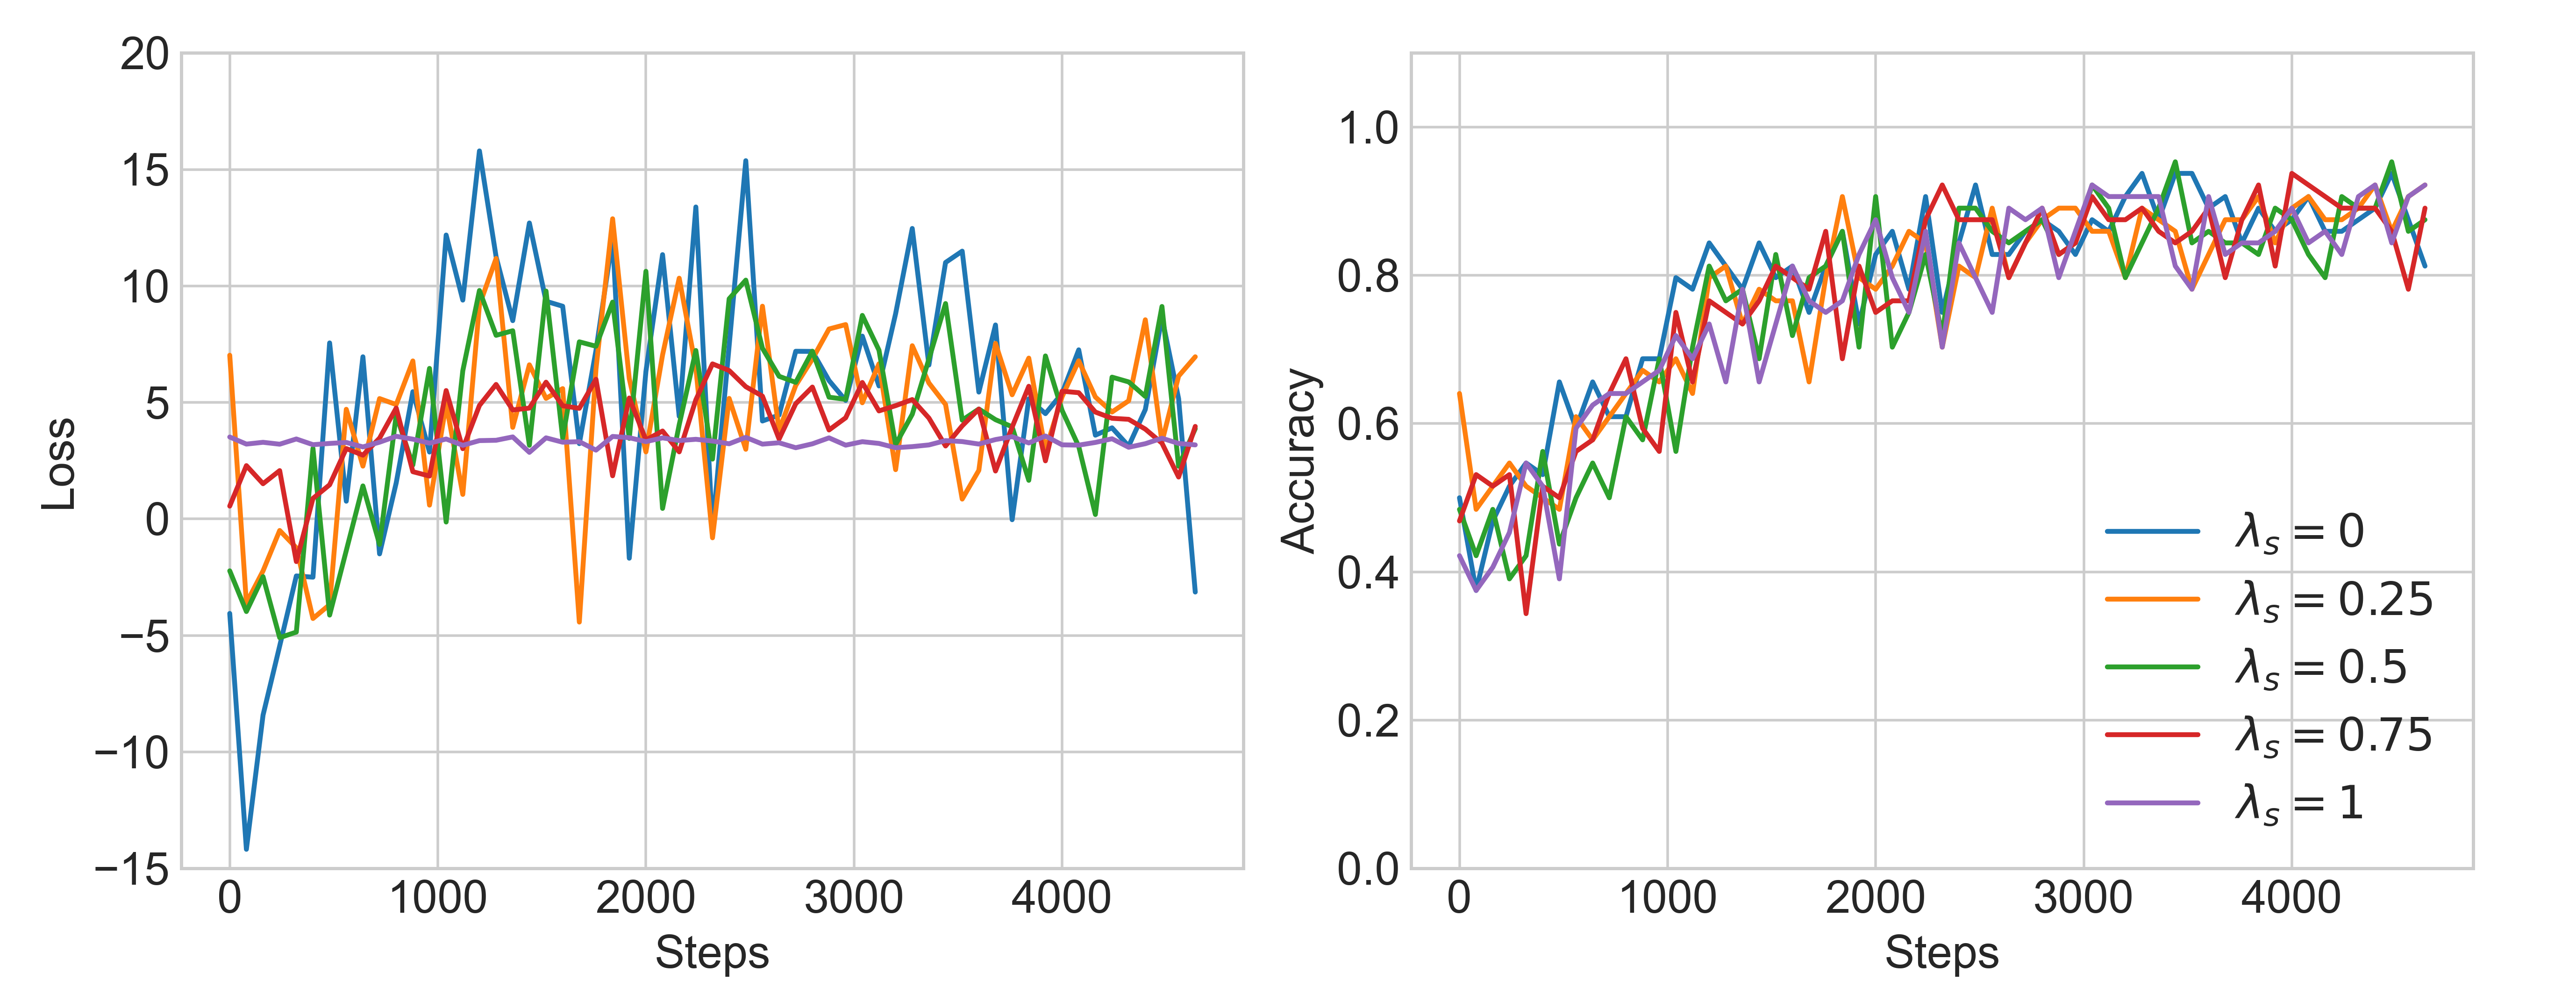
\includegraphics[width=\linewidth]{images/coco_refgame_4000_pure_all_Ls_random.png}
	\caption{Training results of the MS COCO experiment with varying $\lambda_s$ (pure decoding, random pairs). Left: Total speaker training loss. Right: Listener training accuracy.}
	\label{fig:coco_baseline_speaker_loss_listener_acc_all}
\end{figure}

Table \ref{tab:coco_drift_metrics_basic} also provides a comparison of the drift metrics for the different loss configurations. Based on naive comparison, if anything, the structural and semantic drifts were smaller when the structural pressure on the speaker was \emph{smaller}, contrary to a priori intuition. That is, when the pressure to stay close to the initially learned image captioning language distribution was smaller, the produced messages had a higher likelihood both under the pretrained LM and the pretrained speaker. The rather unclear differences between the drift results are also supported by the drift dynamics computed during training (see Fig. \ref{fig:coco_baseline_str_sem_drift_all}). 
The drift values for the experiment with $\lambda_s = 0$ also speak against \textbf{H1} and \textbf{H2}. Somewhat surprisingly, semantic drift values were lower for the generated captions compared to the ground truth captions (Fig.~\ref{fig:coco_baseline_str_sem_drift_all}), indicating that the generated captions were generally more likely given the target image, than the ground truth captions, under the pretrained speaker model. This could be attributed to the auto-regressive pretraining of the speaker, which might have resulted in generally better performance on messages produced in the auto-regressive generation mode, compared to ground truth (see Appendix \ref{app:grid_search} and Section \ref{architecture}).
\begin{figure}
	\centering
	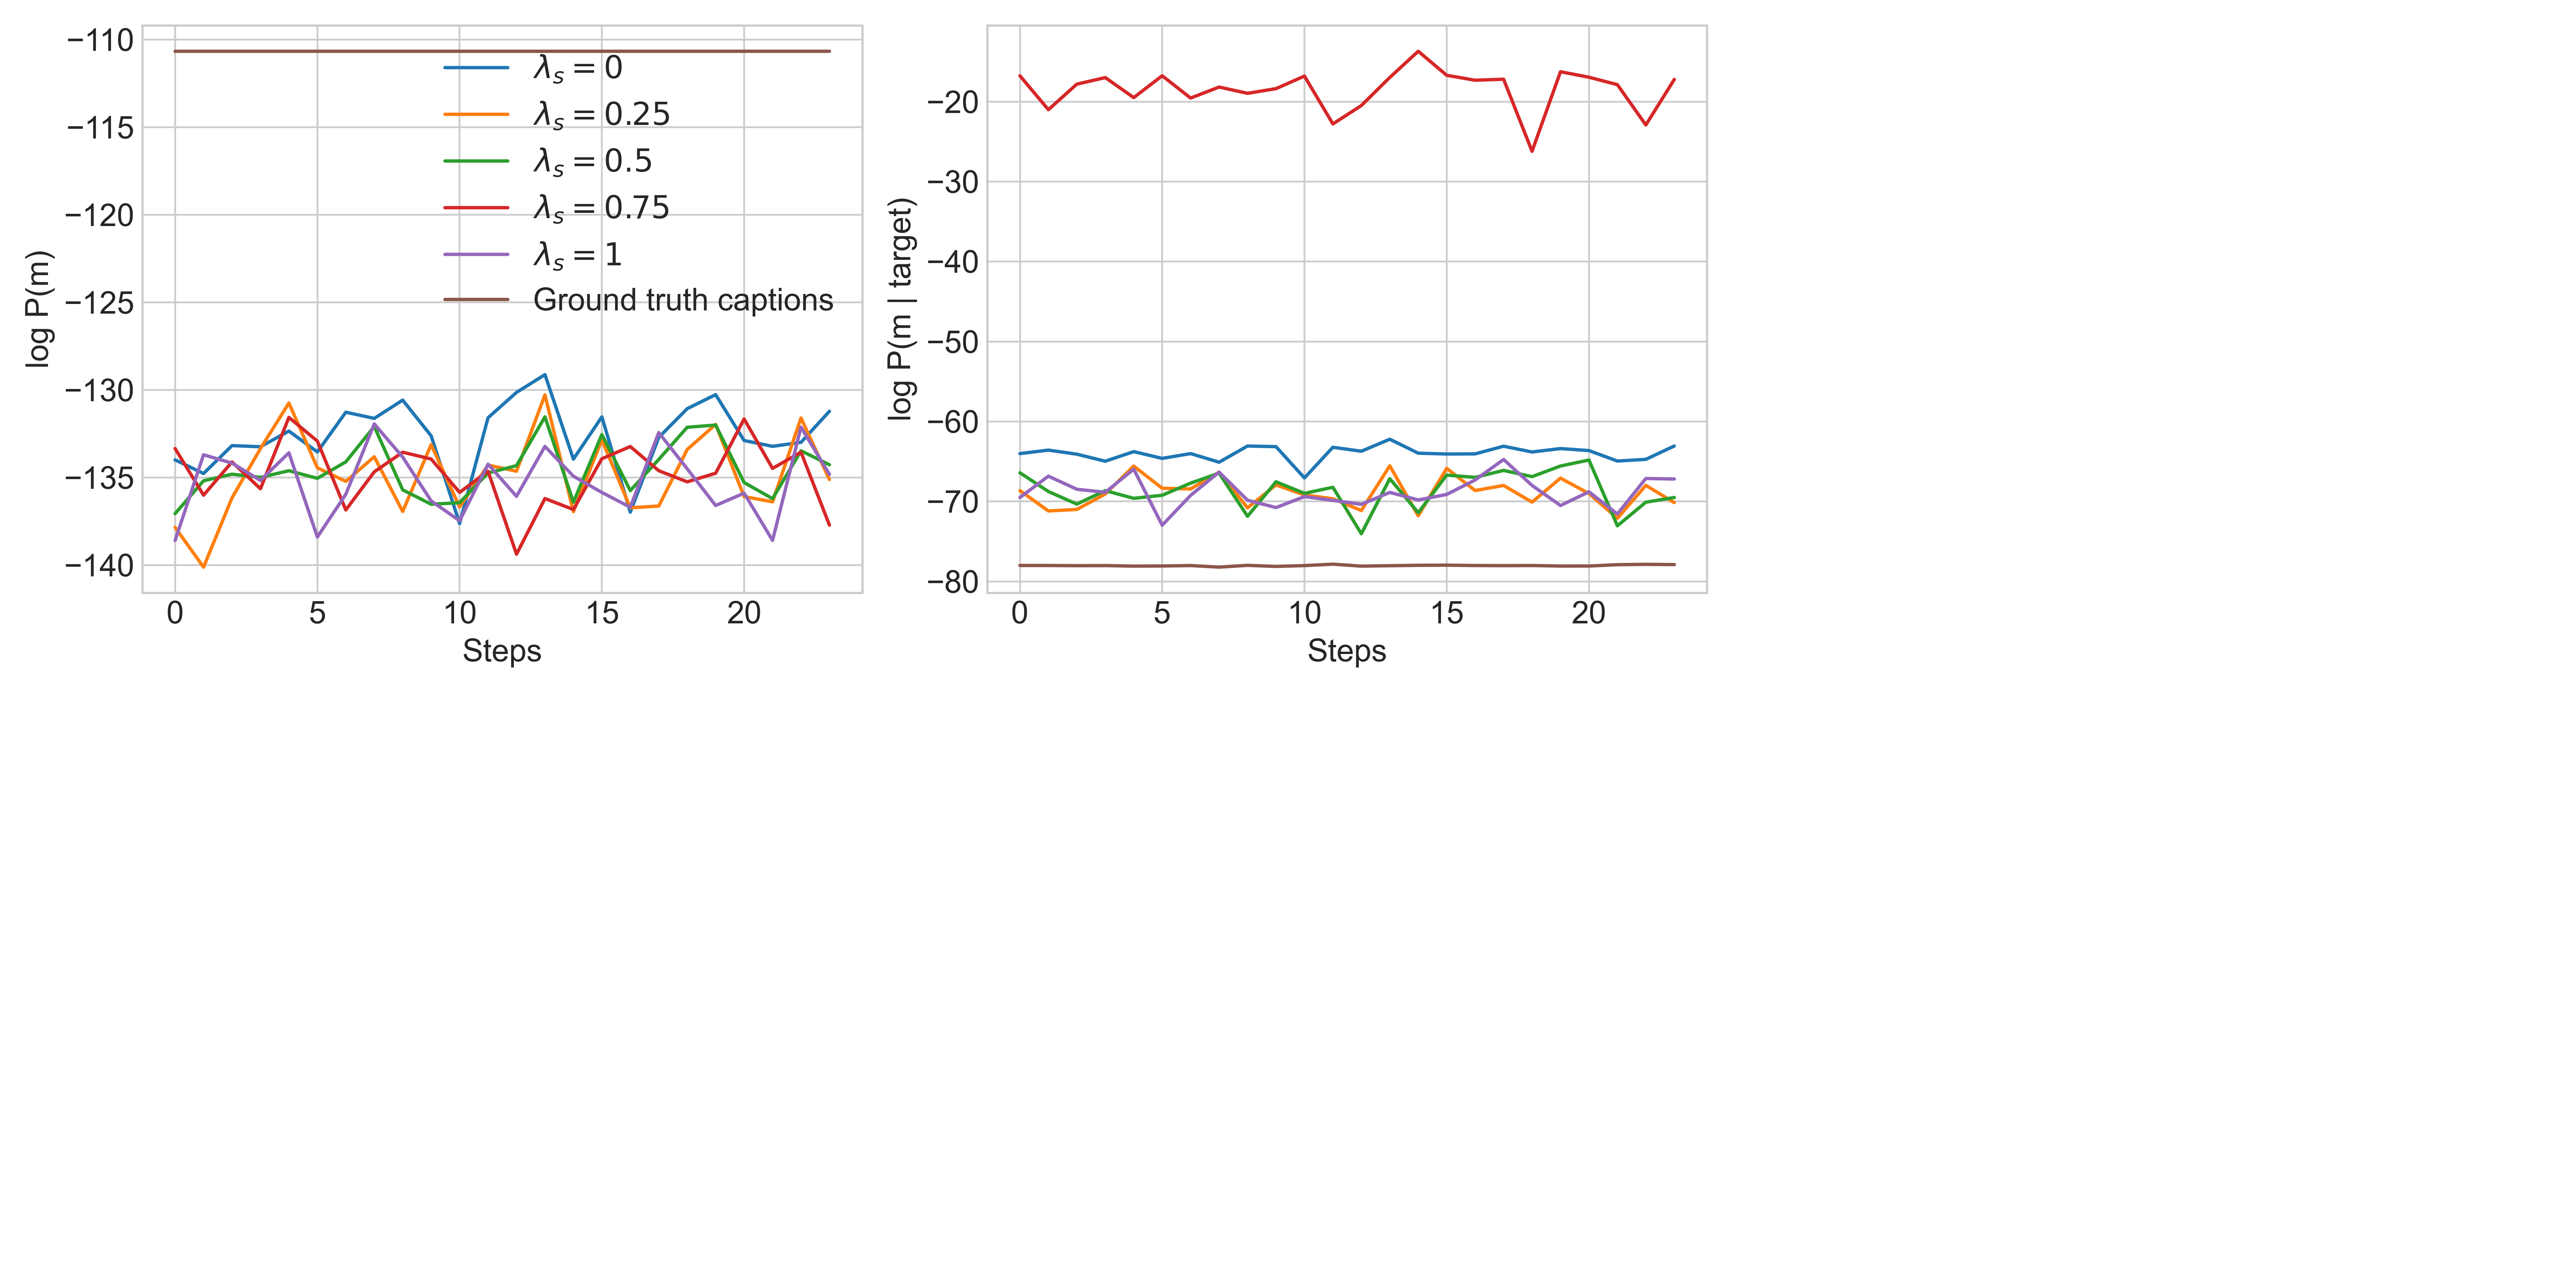
\includegraphics[width=\linewidth]{images/coco_structural_semantic_drift_4000_pure_L_S_all_random.png}
	\caption{Drift dynamics computed during training in the baseline MS COCO experiments (pure decoding) with varying $\lambda_s$ weights. Left: Structural drift of ground truth and predicted captions under the pretrained LM. Right: Semantic drift of ground truth and predicted captions under the pretrained speaker model. Due to a coding error, the semantic drift of the $\lambda_s = 0.75$ model is represented as the mean validation conditional log probability from Tab.~\ref{tab:coco_drift_metrics_basic}.}
	\label{fig:coco_baseline_str_sem_drift_all}
\end{figure}

One reason for the structural drift results might be that the model trained with \emph{less} structural pressure produced messages that were more likely under a pretrained language model. As noted above, the pretrained speaker produced messages that were not very well-formed on a surface level (see Fig.~\ref{fig:coco_randPairs_speaker_generations} for examples), most likely due to the involvement of the auto-regressive pretraining mode (see Appendix \ref{app:grid_search}). Therefore, it might be expected that a speaker which was more strongly forced to stay close to the pretraining language distribution produced less structurally well-formed sentences, under a pretrained LM. The more functionally oriented speaker, on the other hand, might by chance produce better sentences, even if the respective learning signal is not related to the LM. Lastly, it could be hypothesized that these drift results are rather snapshots of the speaker's performance, especially for the speakers with lower $\lambda_s$, since their policies did not converge after training the agents for only two training epochs, as can be seen from the respective loss plot (Fig. \ref{fig:coco_baseline_speaker_loss_listener_acc_all}, left). 
Turning towards the other drift metrics in Table \ref{tab:coco_drift_metrics_basic}, again, there is no indication of a clear trend in connection to the structural loss weight. Nevertheless, the discrete overlap has the highest value for the $\lambda_s = 0$ experiment (0.065 higher than for the pretrained speaker), indicating that the strong functional pressure on the speaker might have led to generating captions capturing more of the target image's properties.

To sum up, given the presented training configurations, \textbf{H4} is not supported by the results. However, based on the grid search over speaker configurations conducted prior to the main experiments (see the difference in reference game performances in Appendix \ref{app:grid_search}, Fig.~\ref{fig:coco_grid_Ls_decoding_TF_only}), one might hypothesize that the presence of effects of the structural loss weight is connected to the presence of auto-regressive pretraining of the speaker agent. That is, it could be critical that the speaker is already pretrained with the caption generation mode, as it then plays a role for the structural loss computation in the reference game. Follow-up experiments regarding this effect of pretraining mode would fill a gap in extant literature \parencite[but see][for related work]{lowe2020interaction}.

\subsection{MS COCO: Similar Pairs Experiments}
\label{expt:coco_similar_pairs}

\begin{figure}[h]
	\centering
	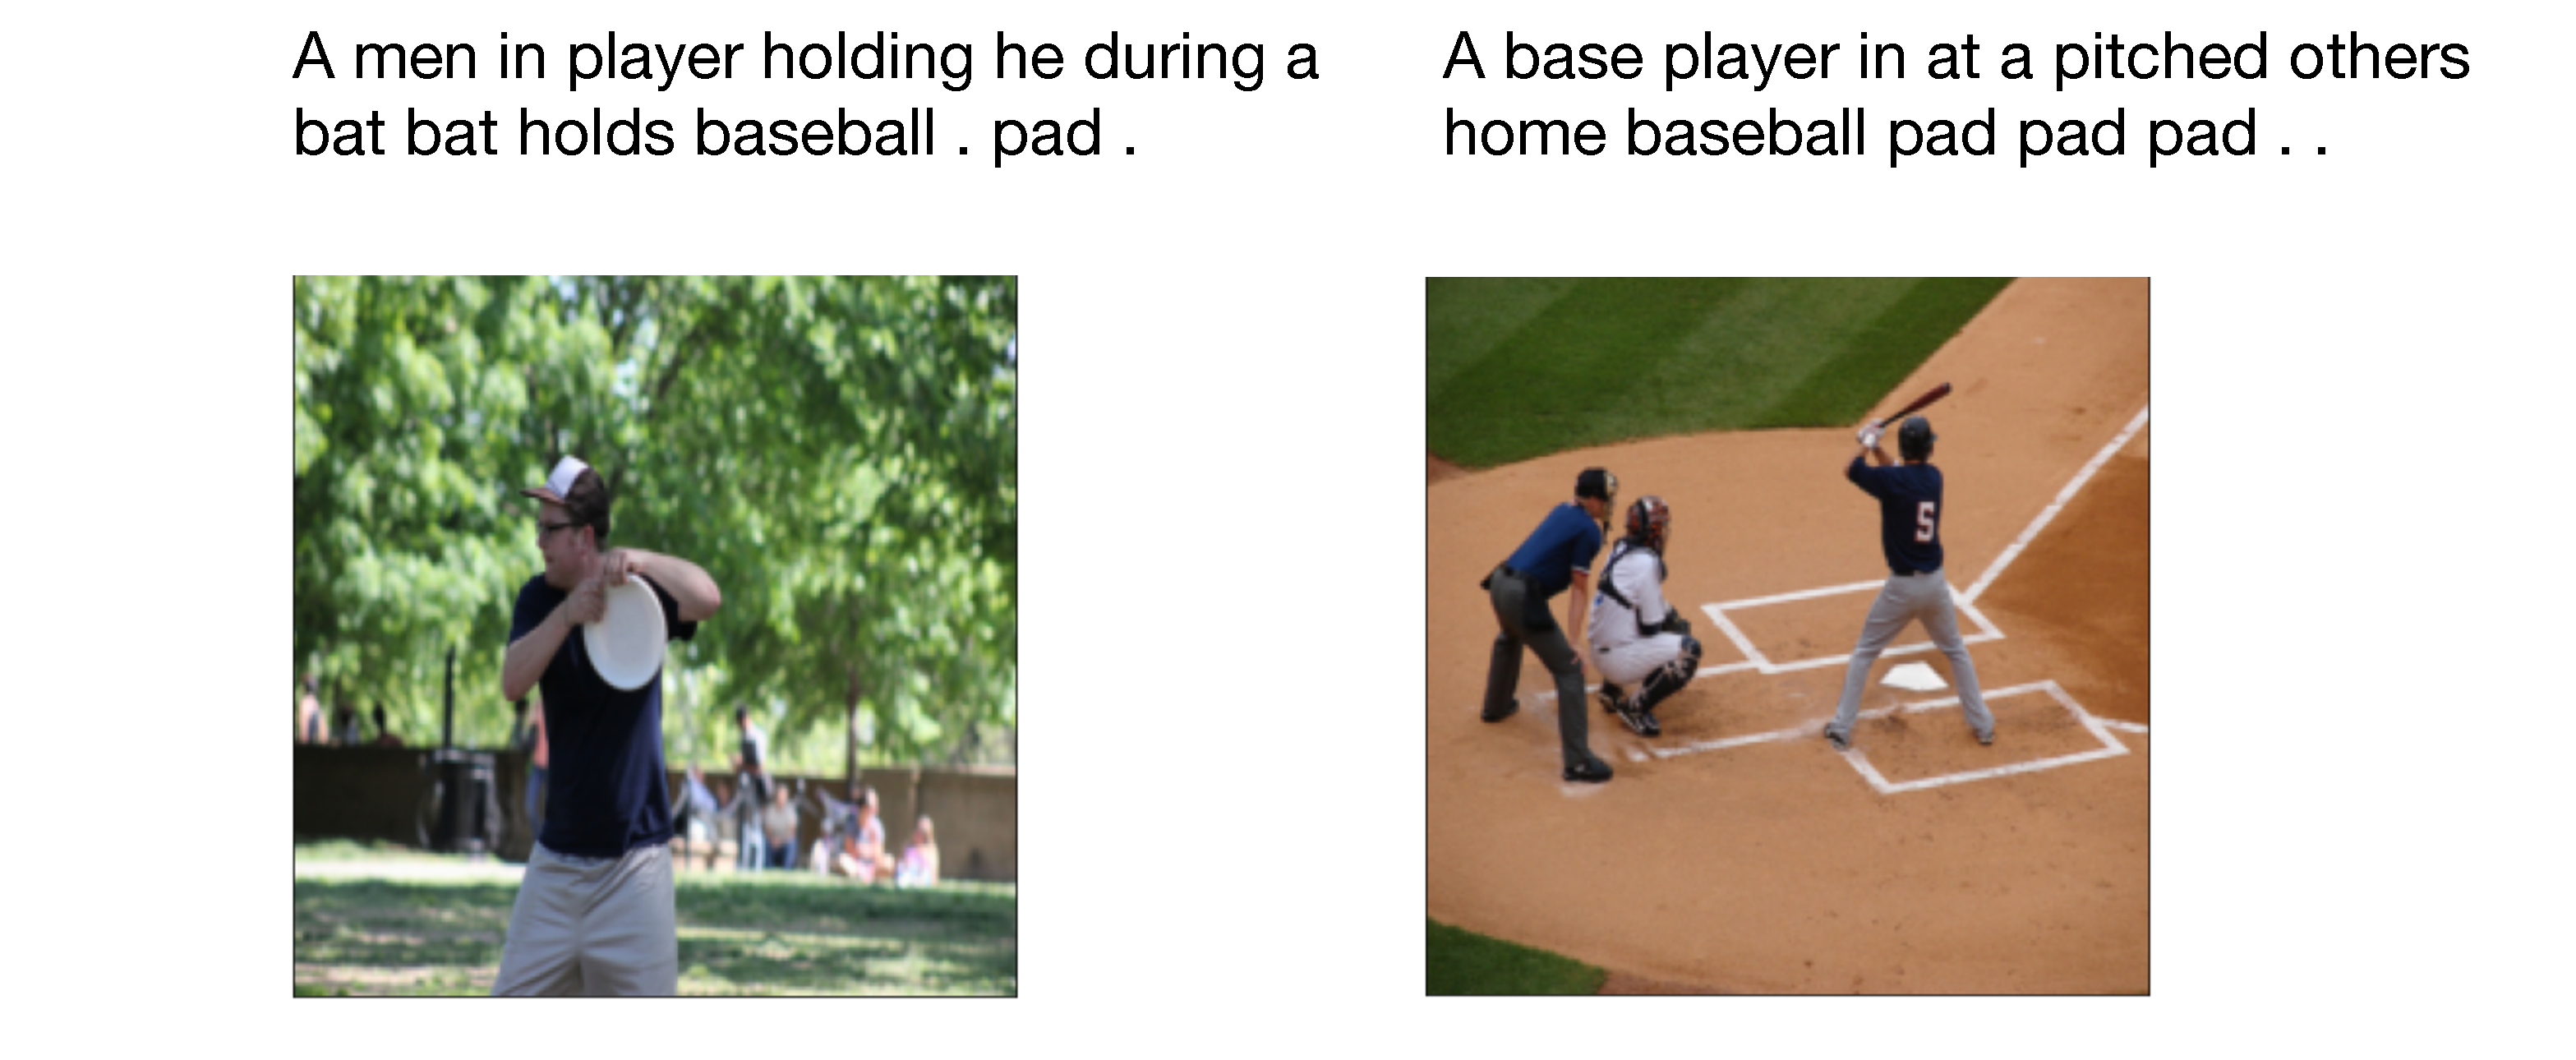
\includegraphics[width=0.8\linewidth]{images/example_generations/coco_speakers_SimilarPairs_example_cropped.pdf}
	\caption{Example message generated by the speaker trained on similar pairs, given a new similar image pair. Messages were generated by treating each image as the target in context of the other image as the distractor.}
	\label{fig:coco_similarPairs_speaker_generation}
\end{figure}
In order to investigate \textbf{H5}, an experiment with similar image pairs was conducted. That is, the goal was to increase the similarity of target and distractor images and thereby increase the pressure to produce more specific messages in reference to the target \parencite[cf.][]{graf2016animal}. As described in Section \ref{ds:coco}, the pairs were constructed by picking the ones depicting at least three identical basic-level categories, as provided by the dataset annotations. Therefore, arguably the similarity of the images was conceptual, which also likely implied a certain degree of perceptual similarity. In order to validate experimental results, similar to the random pairs experiments, the agents' task performance and language drift were tested on 1000 held out \emph{similar} image pairs.\footnote{Drift computations performed during training for monitoring the dynamics were, however, done with random image pairs (for all similar pairs experiments, including 3Dshapes).}
Otherwise, the training configurations matched the baseline experiment. 

\begin{figure}[h]
	\centering
	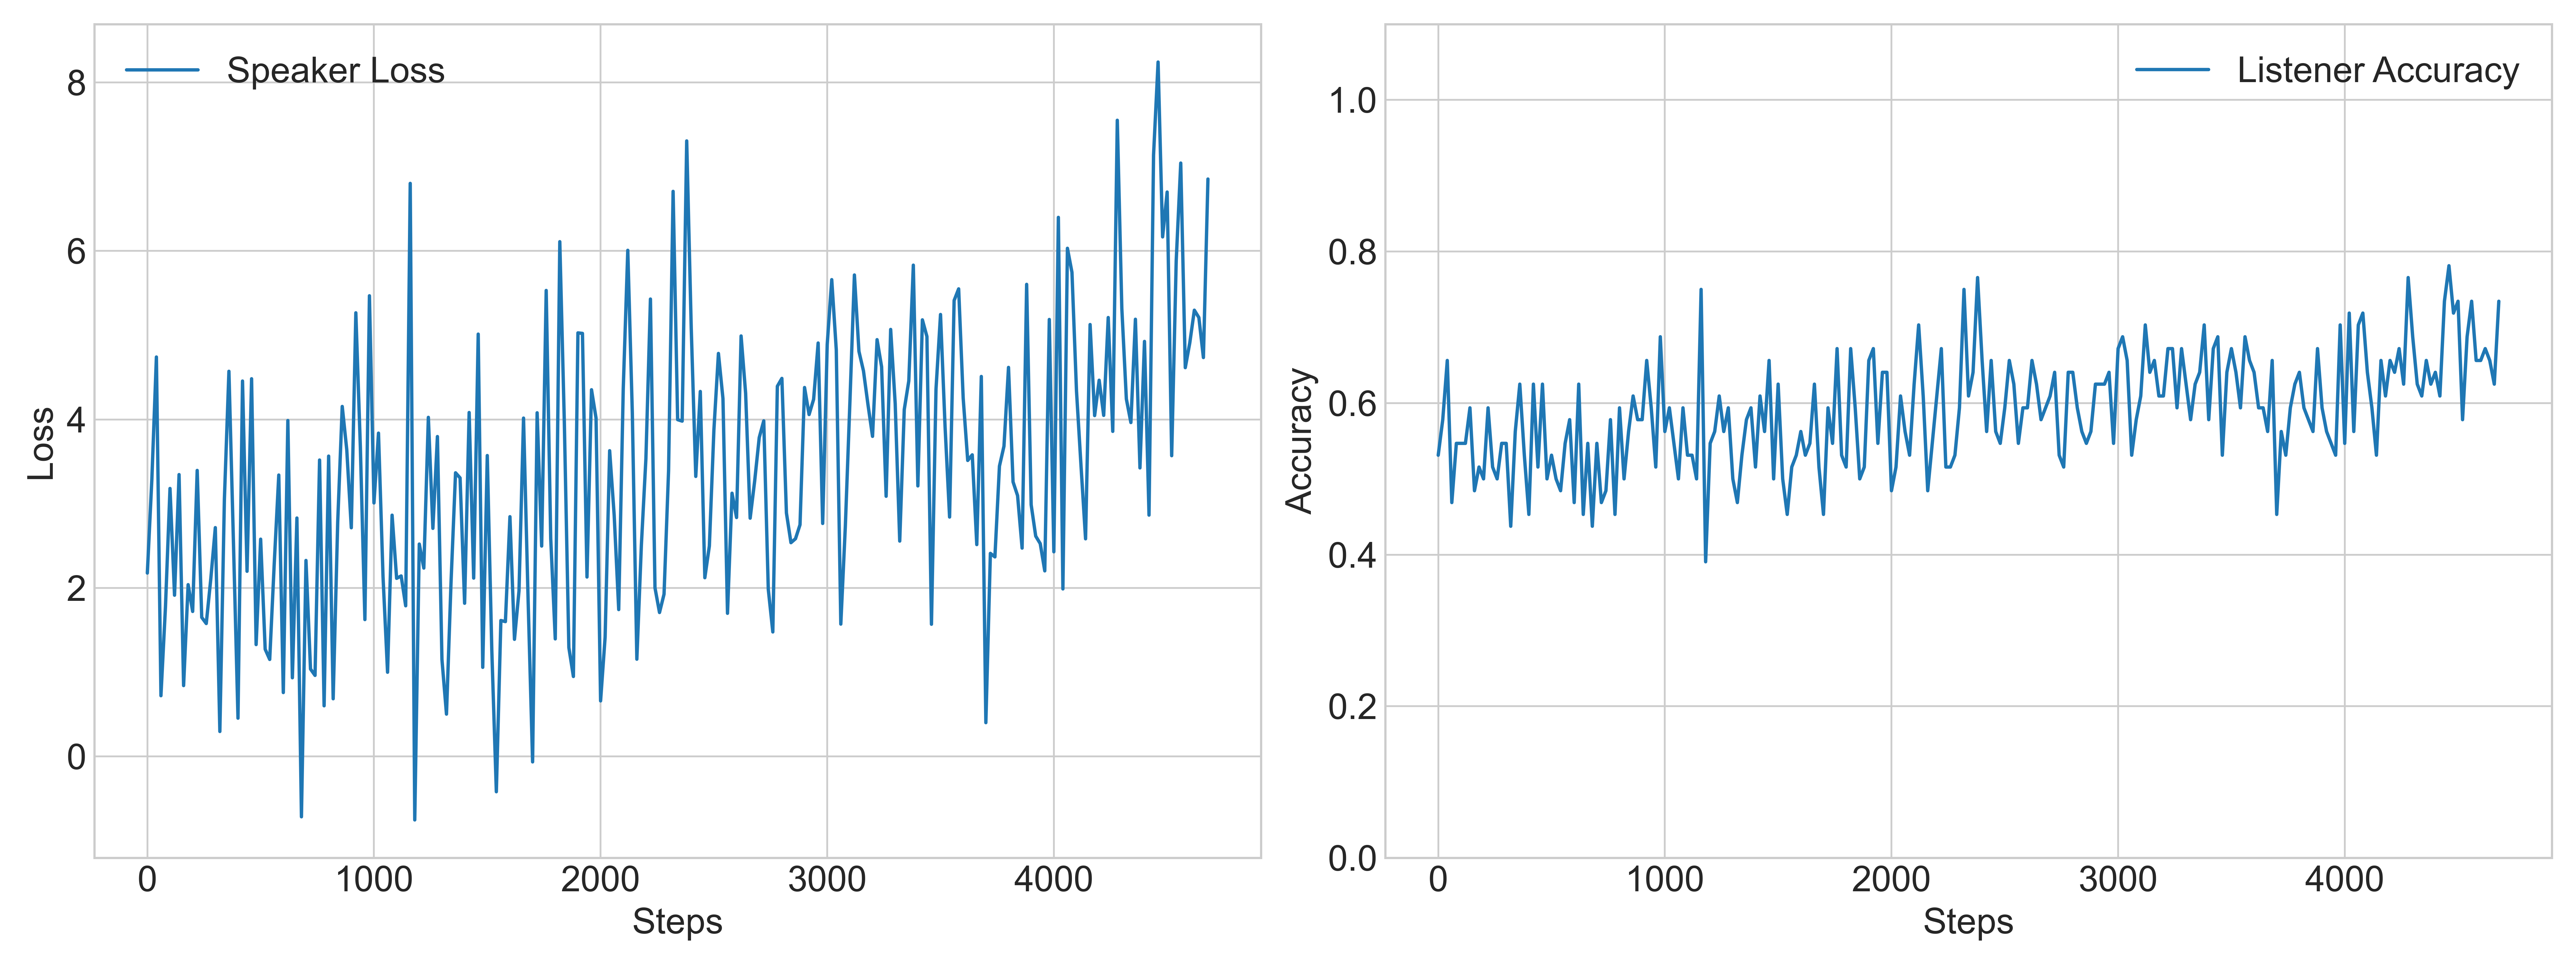
\includegraphics[width=\linewidth]{images/coco_similarFixed_075_losses.png}
	\caption{Training results of the MS COCO experiment with similar target-distractor image pairs ($\lambda_s=0.75$, pure decoding). Left: Total speaker training loss. Right: Listener training accuracy.}
	\label{fig:coco_similar_speaker_loss_listener_acc_all}
\end{figure}

\begin{figure}[h]
	\centering
	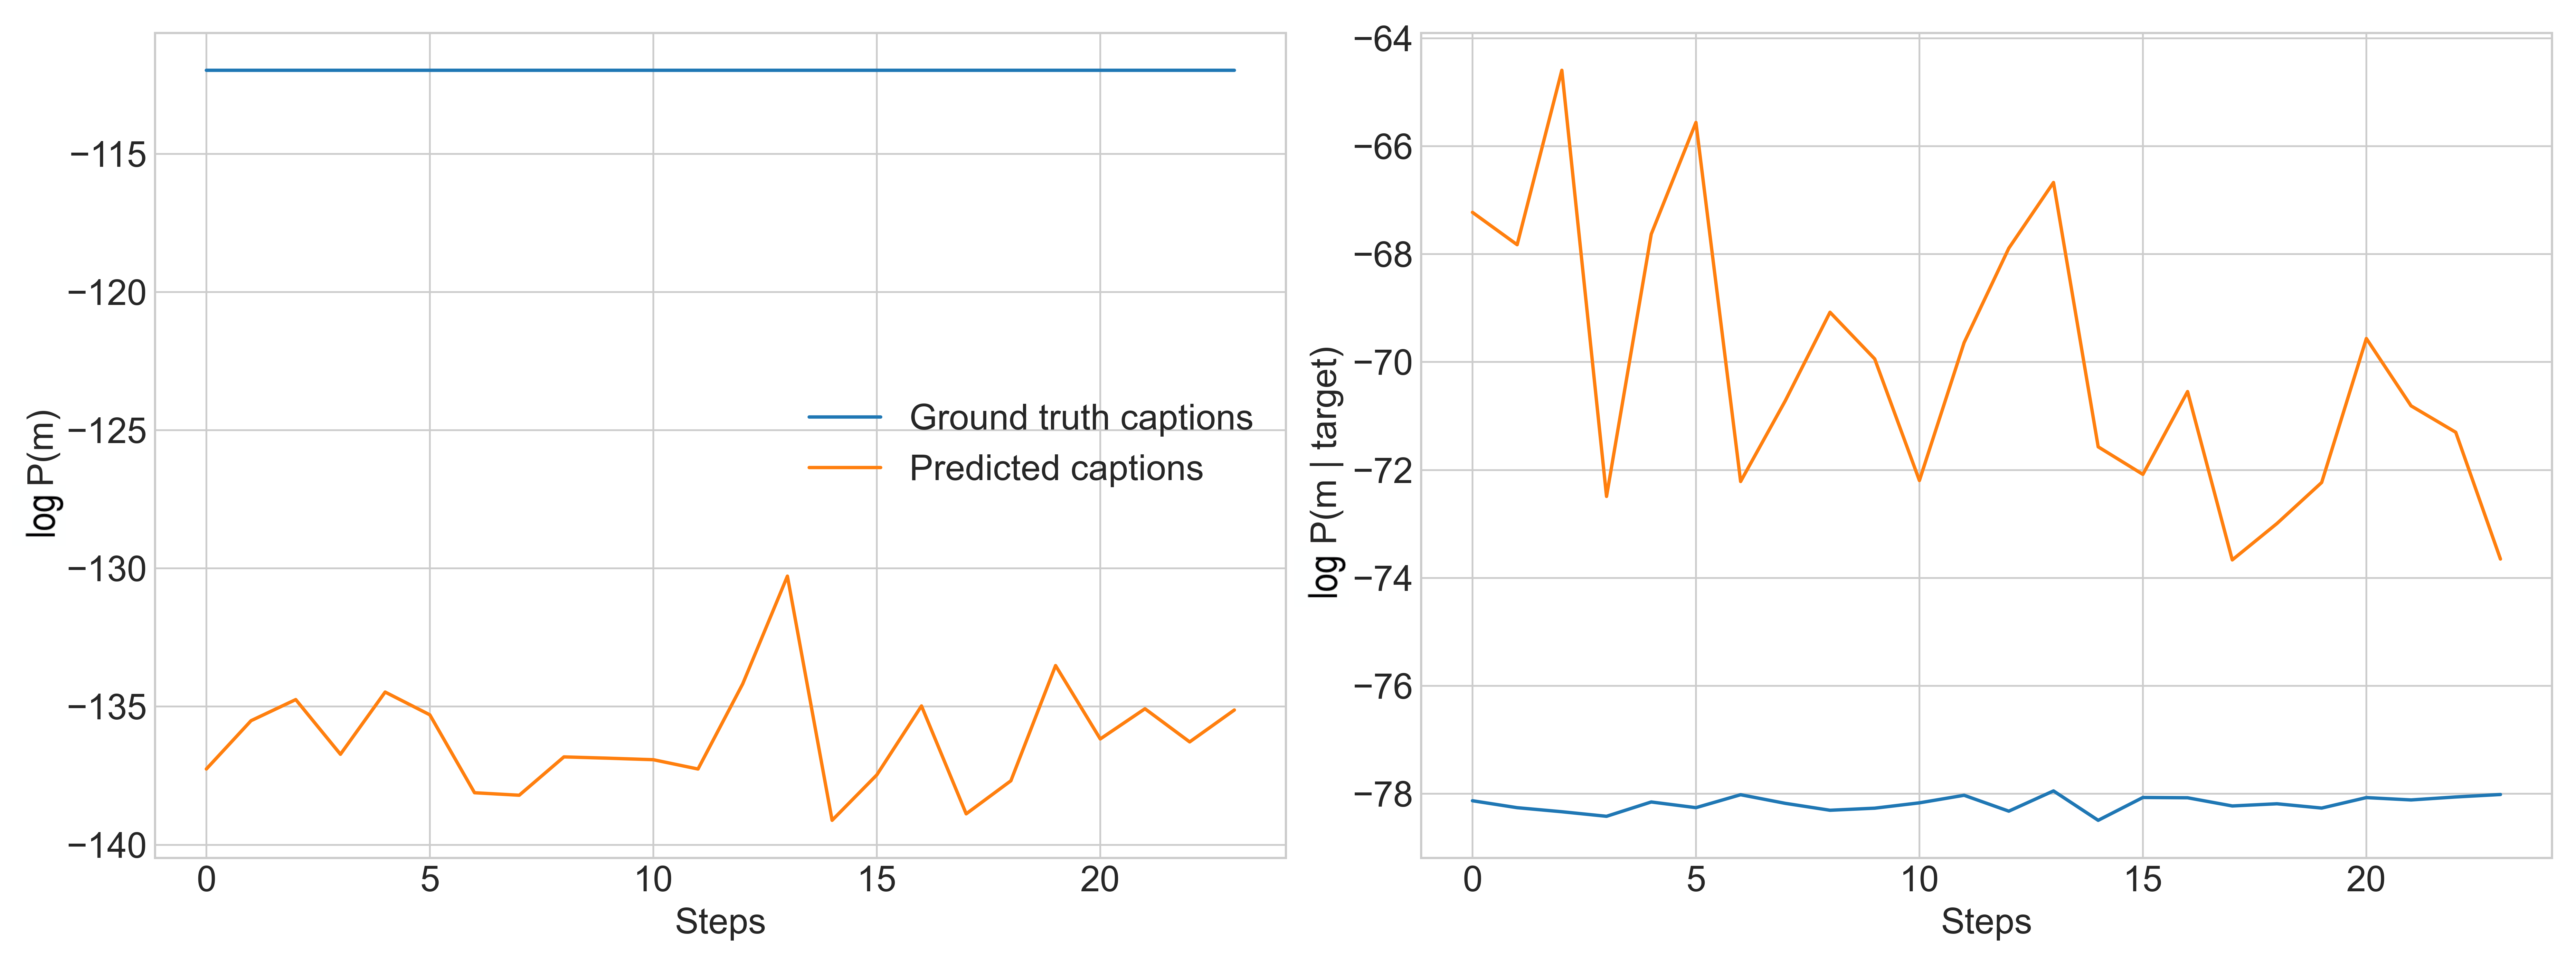
\includegraphics[width=\linewidth]{images/coco_structural_semantic_drift_4000_pure_075_similarFixed.png}
	\caption{Drift dynamics computed during training on similar target-distractor image pairs on MS COCO experiments (pure decoding, $\lambda_s=0.75$). Left: Structural drift of ground truth and predicted captions under the pretrained LM. Right: Semantic drift of ground truth and predicted captions under the pretrained speaker model.}
	\label{fig:coco_similar_str_sem_drift_all}
\end{figure}

Figure \ref{fig:coco_similar_speaker_loss_listener_acc_all} shows the training dynamics of this experiment; compared to the baseline experiment (Fig.~\ref{fig:coco_baseline_speaker_loss_listener_acc_all}, red lines), it is clear that it was much more difficult for the agents to learn the reference game. In fact, visually, they only started improving on the task towards the end of the two training epochs, suggesting that they should be trained longer. This difficulty to learn the task can be attributed to the difficulty of grounding the listener in perceptually similar images with messages which are likely applicable to both images to some extent, making the functional training signal rather weak. This is confirmed by a low listener test accuracy of 0.648, compared to random pairs experiments (Tab.~\ref{tab:coco_drift_metrics_basic}). This confirms the agents' sensitivity to the context in which the target occurs. An example of the speaker's messages can be found in Figure~\ref{fig:coco_similarPairs_speaker_generation}.

This difficulty of grounding the listener led to increasing speaker-listener co-adaptation during training, compared to baseline experiments, as shown by the increasing semantic drift (Fig.~\ref{fig:coco_similar_str_sem_drift_all}, right). This means that instead of learning the `ground truth' meaning of the speaker's words, the listener and the speaker built new conventions, more effective for this similar input. No such trend is visible for structural drift (Fig.~\ref{fig:coco_similar_str_sem_drift_all}, left); its dynamics are comparable to the baseline experiments (Fig.~\ref{fig:coco_baseline_str_sem_drift_all}, left). 
However, both structural and semantic language drift on the test set were lower for the similar pairs than for the random pairs experiments, indicating that it is the strength of the functional signal that was likely responsible for both structural and semantic drift. That is, since it was more difficult for the listener to learn the task and, therefore, the task-based feedback to the speaker was less conclusive than for random pairs, the speaker did not adapt her messages as strongly.
At the same time, the decrease in discrete overlap indicates that it was more difficult for the speaker to find words that are true of the target but not the distractor. On the other hand, the decrease might also indicate that the speaker might have learned to mention more novel features of the target which were not part of the ground truth caption, compared to random pairs experiments and the pretrained speaker. Following the idea behind this value as a functional drift metric, it decreased with decreasing task success, compared to the random pairs experiment value. No clear difference in continuous overlap compared to random experiments was observed.

\begin{figure}[h]
	\centering
	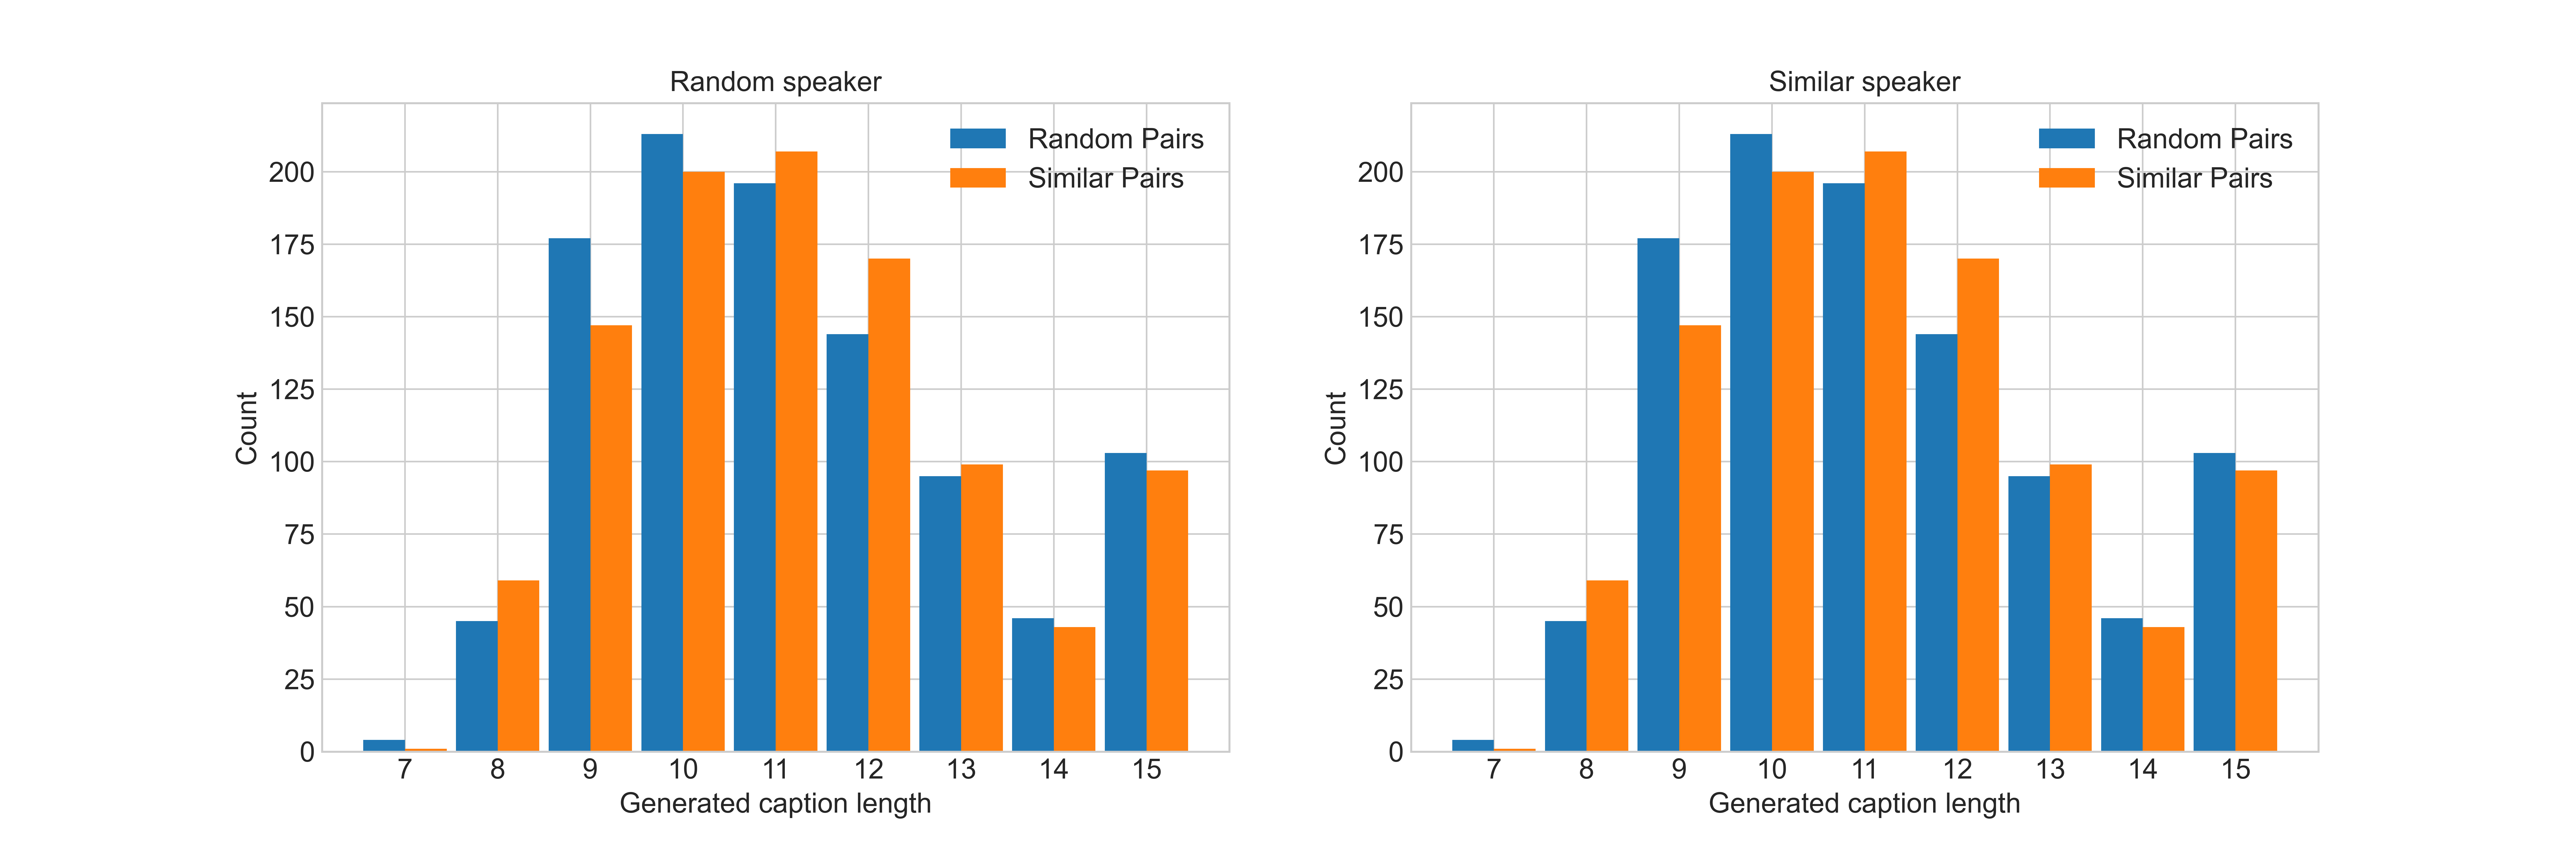
\includegraphics[width=\linewidth]{images/coco_random_similar_length_counts.png}
	\caption{Distribution of produced sentences' lengths given similar and random target-distractor image pairs. Left: Speaker trained on the baseline random pairs reference game. Right: Speaker trained on the similar pairs reference game.}
	\label{fig:coco_similar_random_speaker_lengths}
\end{figure}
In order to investigate the second part of \textbf{H5}, namely whether the specificity of the speaker's messages in the similar pairs experiment increased, the lengths of the messages generated on the test set were investigated. To this end, the number of tokens until the first special \texttt{END} token was computed (excluding it). The lengths of messages generated by the speaker from the baseline experiment (Section \ref{expt:coco_baseline}) was compared to those of the speaker from this experiment, given similar test image pairs versus random test image pairs (Fig.~\ref{fig:coco_similar_random_speaker_lengths}). The figure shows a slight trend towards longer messages for similar images pairs, suggesting that, supporting the hypothesis, the speaker used more words in order to refer to more difficult targets. However, it also suggests that this was the case for both speakers, i.e., that this tendency did not emerge due to exposure to similar training pairs in this experiment compared to the random baseline, but rather might be the result of speaker pretraining (cf.~Section~\ref{speaker_pretraining}). Because they were pretrained on pairs of images, it might be the case that the speakers implicitly learned to put the target in context of the distractor, and, therefore, produced this trend.
\begin{figure}[h]
	\centering
	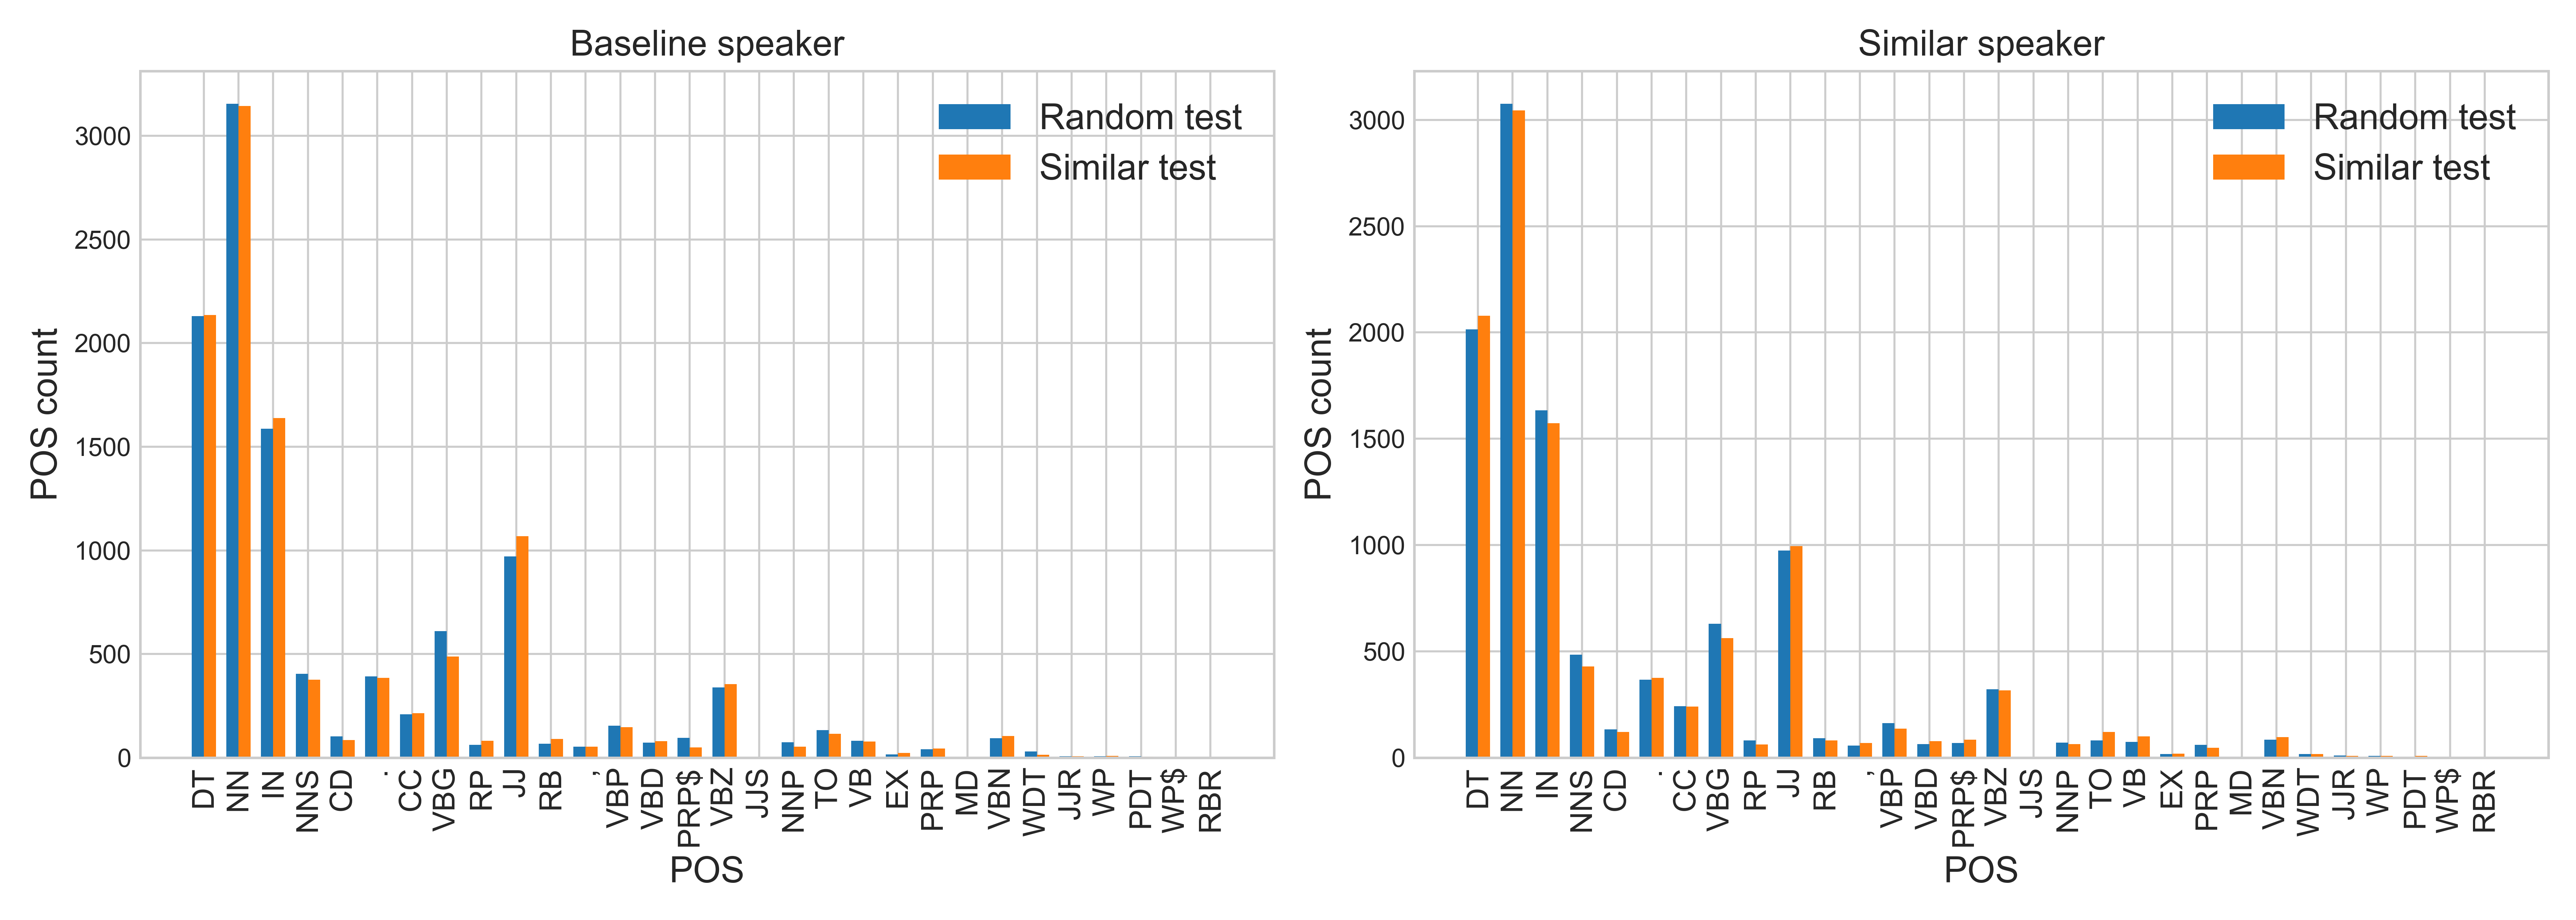
\includegraphics[width=\linewidth]{images/coco_similar_v_baseline_randomTest_vs_similarTest_POS_counts.png}
	\caption{Distribution of POS tags in produced sentences lengths given similar and random target-distractor image pairs. Left: Speaker trained on the baseline random pairs reference game. Right: Speaker trained on the similar pairs reference game.}
	\label{fig:coco_similar_random_speaker_POS}
\end{figure}
To further zoom in on the granularity of the productions, the produced messages were tagged with parts of speech (POS) tags with the \texttt{nltk} package \parencite{bird2006nltk} and the distribution of the tags was compared for the baseline and this experiment. Figure \ref{fig:coco_similar_random_speaker_POS} shows that the were small differences in the parts of speech preferred for either type of image pairs, but no decisive trends or differences between the baseline speaker and the speaker from the similar pairs experiment are visible. This also indicates that differences may potentially rather stem from the pretrained speaker's sensitivity towards the distractor. Additionally, taken together, these analyses indicate that the speaker of the similar pairs experiment did not learn particular strategies of referring to the target, compared to random image pairs, which most likely may be due to the complexity of the task and the short reference game training time.

Additionally, the speaker was also evaluated with standard image captioning metrics. Table \ref{tab:eval_metrics_refgame} shows that caption quality visibly decreased with respect to all metrics, showing the difficulty to produce correct captions for targets given similar distractors in an even more pronounced way than the drift metrics.

To sum up, these results support \textbf{H5} in that the speaker's messages are less discriminative given more similar target-distractor pairs. They do not provide conclusive evidence that the speaker produced more granular messages for similar image pairs. They nonetheless confirm that the agents are highly sensitive to the visual context of their task.

\subsection{MS COCO: Fixed Listener Experiments}
\label{exp:coco_fixed_listener}
In order to investigate \textbf{H6}, a reference game with random pairs and $\lambda_s=0.75$ was conducted with a \emph{fixed} listener. That, is the speaker was fine-tuned to produce discriminative captions while being provided the task success signal by an already pretrained listener which was not further trained during the reference game, as opposed to receiving the task success signal from a \emph{joint} listener which learns to complete the task and ground the speaker's messages during the reference game. To this end, the listener was pretrained for four epochs to optimally interpret ground truth image captions. The same images as for the speaker pretraining were used. That is, the listener agent saw random pairs of images and received the ground truth caption for the target and was optimized to identify the target. After pretraining, the fixed listener's test accuracy on the ground truth captions of a held out dataset of 1000 images was 0.963. The test accuracy on messages generated by the pretrained speaker for the same images was 0.902.

The goal of this experiment was to investigate language drift in absence of speaker-listener co-adaptation which arises when the two agents are trained together. By having a fixed pretrained listener, intuitively, the speaker cannot improve the message discriminativity by finding `loopholes' and establishing specific conventions with the listener, and should be forced to use the ground truth grounding of the messages.

\begin{figure}[h]
	\centering
	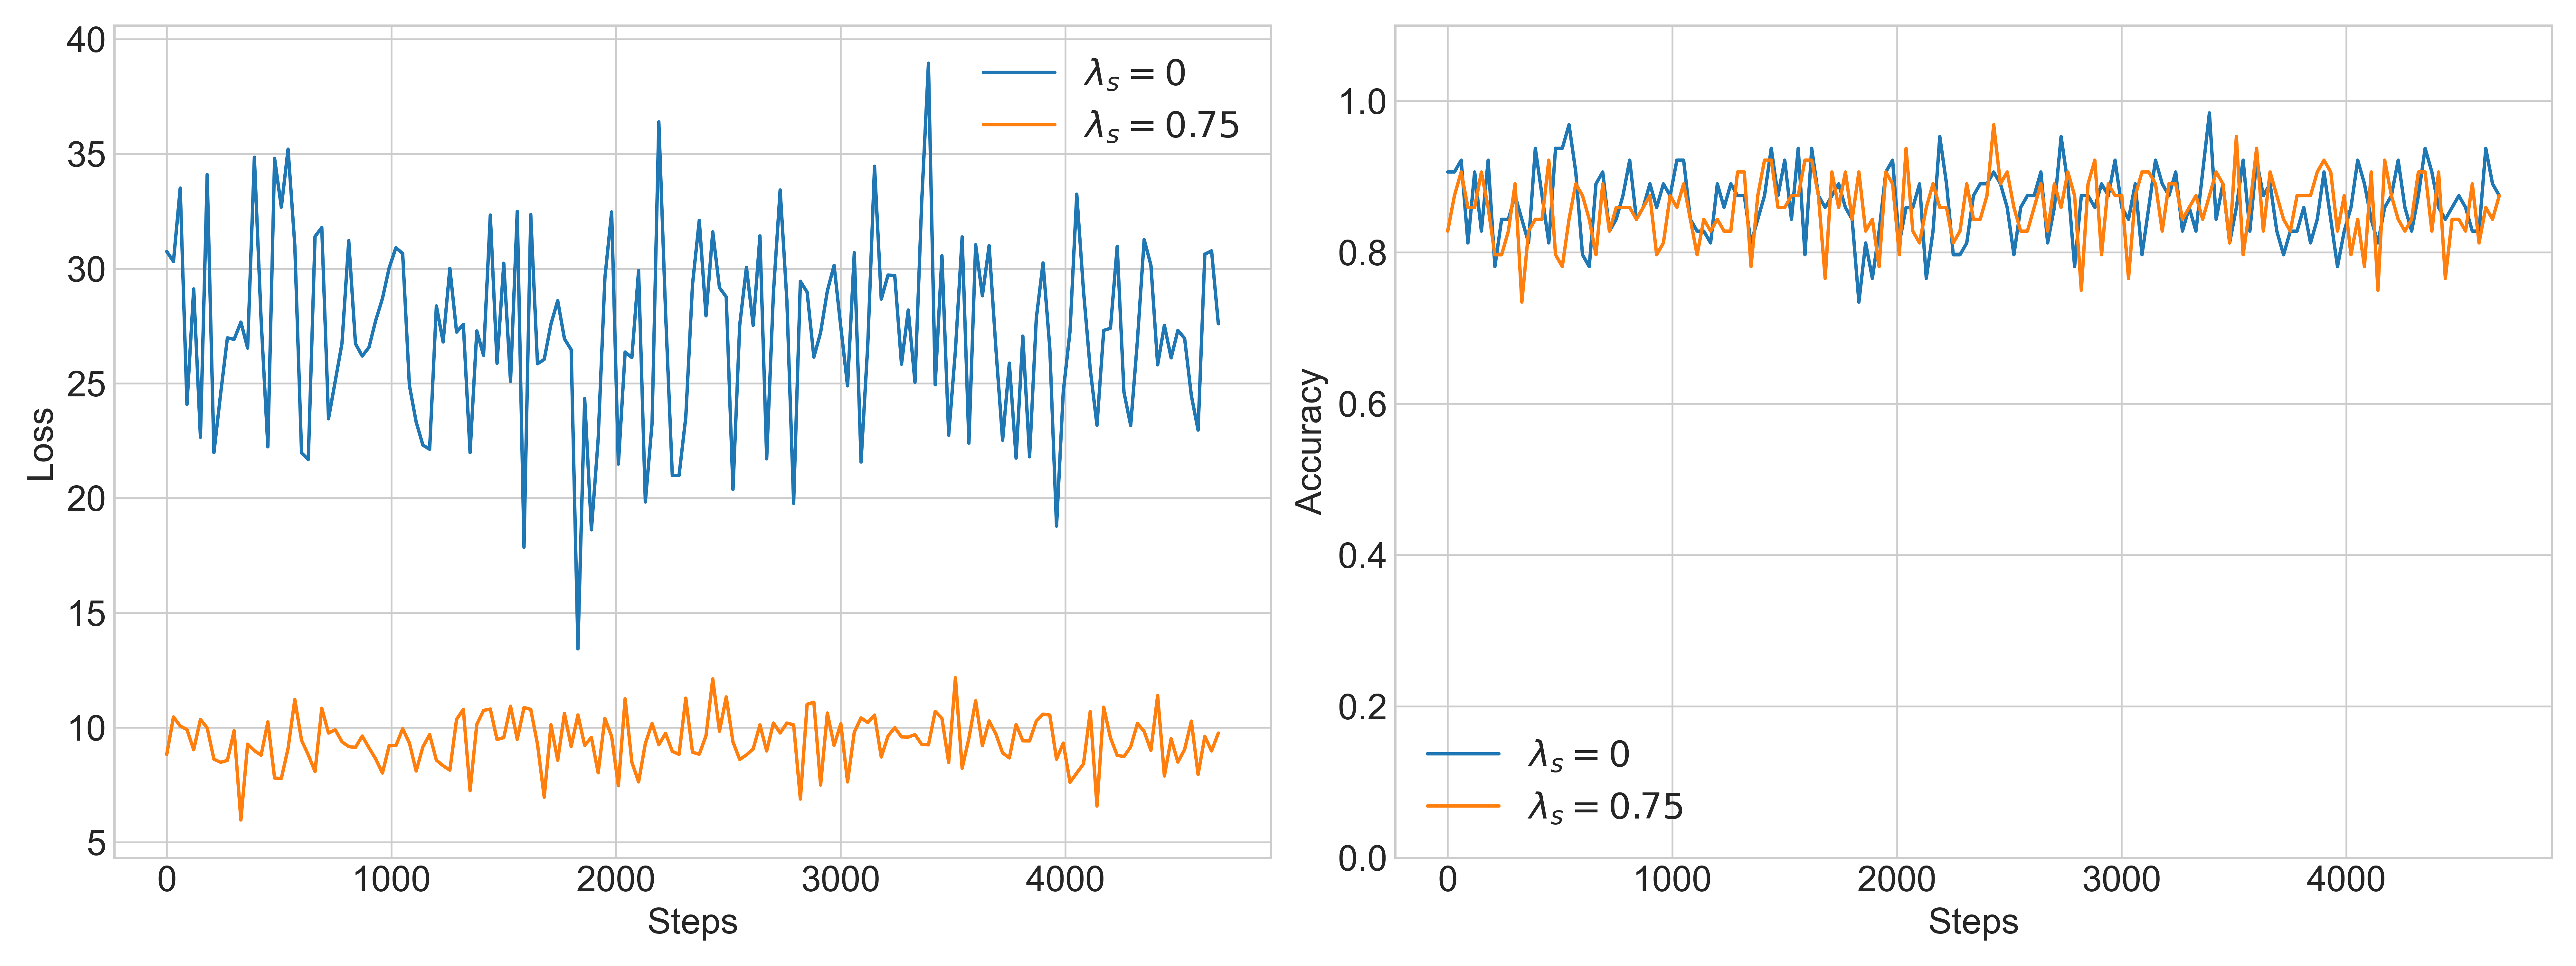
\includegraphics[width=\linewidth]{images/coco_fixedListener_baseline_random_0_075_losses.png}
	\caption{Training results of the MS COCO experiment with a fixed listener (pure decoding, $\lambda_s=0$ vs. $\lambda_s=0.75$). Left: Total speaker training loss. Right: Listener training accuracy.}
	\label{fig:coco_fixed_listener_speaker_loss_listener_acc_075}
\end{figure}

The training and testing procedures were identical to previously described random image pairs experiments. The training dynamics can be seen in Figure \ref{fig:coco_fixed_listener_speaker_loss_listener_acc_075}. They indicate that the task success based training signal was not strong enough in order to visibly improve the task performance beyond literal message interpretation, because the listener's accuracy did not improve beyond the accuracy in responding to the pretrained speaker (right plot). The speaker's policy also did not visibly converge (left plot). 
This is confirmed by the listener test accuracy of 0.881 in Table \ref{tab:coco_drift_metrics_basic}, which additionally indicates that the reference game success is at least partly carried by speaker-listener co-adaptation, since the accuracy decreased by 0.072 compared to the experiment with a jointly trained listener. 

Turning to the language drift metrics in Table \ref{tab:coco_drift_metrics_basic}, it can be observed that training the speaker with a fixed listener indeed mitigated structural and semantic drifts, compared to training with a joint listener (``MS random, fixed listener, $\lambda_s=0.75$'' line~vs.~``MS baseline, random, $\lambda_s=0.75$'' line compared to the ``Pretrained MS speaker''). Consistent with intuitions, the mitigation was stronger for the semantic drift than for structural drift---the log likelihood was 4.192 higher for the former and 1.502 higher for the latter for the fixed listener experiment, compared to the joint one (Tab.~\ref{tab:coco_drift_metrics_basic}). Consistent with the effects of the fixed listener on the apparent absence of functional speaker improvement discussed above, the discrete overlap did not increase compared to the pretrained speaker (and even decreased by 0.152). The continuous overlap did not change compared to the pretrained speaker. The image caption evaluation metrics in Table \ref{tab:eval_metrics_refgame} suggest that the speaker's messages diverged from the ground truth a little stronger than for the pretrained speaker and the joint listener baseline experiment, but the differences seem negligible.%Based on the drift dynamics during the training (Fig.~\ref{fig:coco_fixed_listener_075_str_sem_drift}), one could, however, hypothesize that with longer training, the semantic drift might increase (based on the slightly visible negative trend in the right plot).
\begin{figure}[h]
	\centering
	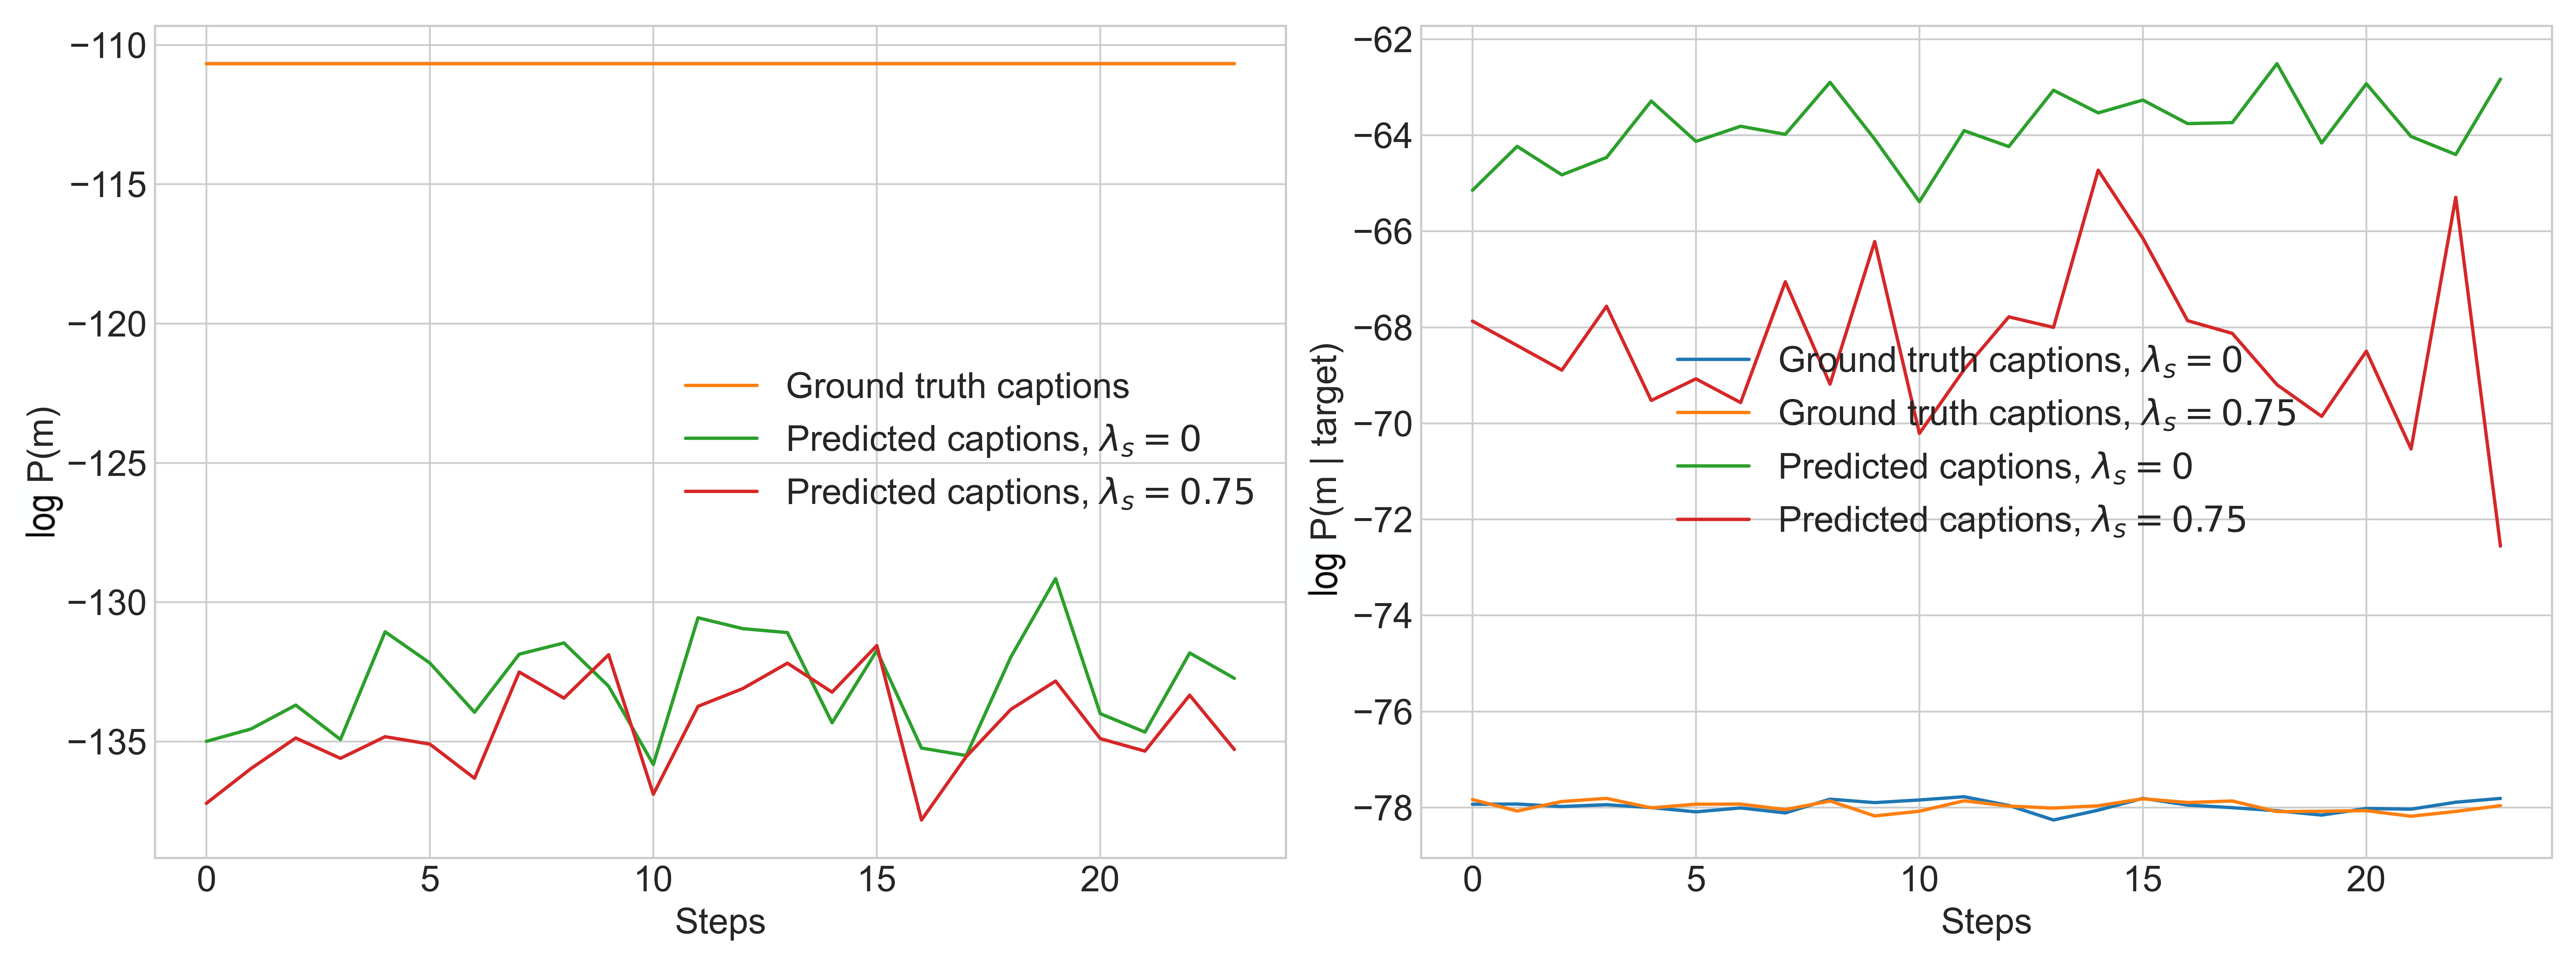
\includegraphics[width=\linewidth]{images/coco_fixedListener_structural_semantic_drift_4000_pure_0_075_random.png}
	\caption{Drift dynamics computed during reference game training with the fixed listener on MS COCO (pure decoding, $\lambda_s=0$ vs. $\lambda_s=0.75$). Higher values indicate less drift. Left: Structural drift of ground truth and predicted captions under the pretrained LM. Right: Semantic drift of ground truth and predicted captions under the pretrained speaker model.}
	\label{fig:coco_fixed_listener_075_str_sem_drift}
\end{figure}

In order to investigate whether task improvement can be achieved without speaker-listener co-adaptation when a stronger functional learning signal is present, a second experiment with $\lambda_s=0$ (i.e., functional learning only) was conducted. While no improvement in terms of task performance is apparent visually (Fig,~\ref{fig:coco_fixed_listener_speaker_loss_listener_acc_075}), there was a little increase in terms of listener test accuracy to 0.888 (Tab.~\ref{tab:coco_drift_metrics_basic}). Furthermore, Table \ref{tab:coco_drift_metrics_basic} indicates that under stronger functional constraints, language drift was mitigated even better, compared to the $\lambda_s = 0.75$ fixed listener. More precisely, structural drift was lower, even outperforming the pretrained speaker. Similarly, semantic drift also narrowly improved beyond both the pretrained and the $\lambda_s = 0.75$ speakers. 
The overlap metrics also slightly improved or remained constant compared to both the $\lambda_s=0.75$ experiment, the jointly trained listener-speaker experiment and the pretrained speaker. These results suggest that when removing the agent co-adaptation, a strong enough functional training signal might yield more discriminative captions which mention more target than distractor features. 

To sum up, the data supports \textbf{H6} for the MS COCO experiment, but also strongly suggests that the functional signal available under the functional loss weight of 0.25 is not sufficient in order to visibly fine-tune the speaker for the task. When increasing the strength of the functional signal from the listener by setting $\lambda_s$ to 0, a tangiable improvement of language drift can be observed, indicating that both grounding and the structure expected by the listener positively affect the speaker.

\subsection{MS COCO: Greedy Decoding Experiments}
\label{expt:coco_greedy}
\begin{table}[]
	\begin{tabularx}{\linewidth}{|X|l|l|X|X|X|}
		\hline
			\textbf{Model name}                                    & \textbf{log $P(m)$} & \textbf{log $P(m \mid i)$} & \textbf{Overlap (d)} & \textbf{Overlap (c)} & \textbf{Acc. }  \\ \hline
			 Baseline random pairs, fixed listener, pure decoding   &     -138.500         &         -74.988               &       1.059            &      0.001               &       0.865       \\ \hline
			 Baseline random pairs, fixed listener, greedy decoding   &     -100.674     &         -36.419              &       1.400       &      0.005             &       0.814         \\ \hline
			 Baseline random pairs, pure decoding   & -136.114        &      -72.959            &       1.065          &      0.002               &       0.550       \\ \hline
			 Baseline random pairs, greedy decoding   &-100.187      &    -35.910            &       1.355          &      0.006            &       0.544       \\ \hline
			 Baseline similar pairs, pure decoding   &     -137.491& -77.898    & 0.198    &   -0.005    &  0.542        \\ \hline
			 Baseline similar pairs, greedy decoding   &   -101.436  &      -38.911        &     0.044   &     0.003     &  0.565           \\ \hline
			 
	\end{tabularx}
\caption{\label{tab:coco_greedy}Language drift metrics and listener test accuracies (``Acc.'') on MS COCO experiments conducted with greedy decoding.}
\end{table}

Finally, as explained in the introduction (see Section~\ref{model_pretraining}), another factor which may influence the performance of the speaker is the decoding strategy. While pure decoding was chosen as the main strategy, this section looks at representative sample experiments employing \emph{greedy} decoding. That is, at each timestep of the generation, the speaker picked the token with the highest probability given the images and preceeding tokens in order to continue her message. 

For gathering representative results, the baseline experiment (random pairs, joint listener, $\lambda_s=0.75$), the similar pairs experiment (joint listener, $\lambda_s=0.75$) and a fixed listener experiment (random pairs, $\lambda_s=0.75$) were replicated with the greedy decoding strategy. Training results in Figure~\ref{fig:coco_greedy_baseline} indicate that for the joint listener experiments, the agents failed to learn the reference game (i.e., their training performance remained at chance level 0.5). Since the speaker and the fixed listener were able to play the game, the reason for failure in the other two experiments most likely was the inability to ground the joint listener. That is, the listener could not pick up how the speaker described the target, both for random and similar target-distractor pairs. This is corroborated by nearly chance-level listener test accuracy (Tab.~\ref{tab:coco_greedy}). For all three experiments, the test performance with greedy decoding on the test set was compared to test performance with pure decoding on the same set. 
\begin{figure}[h]
	\centering
	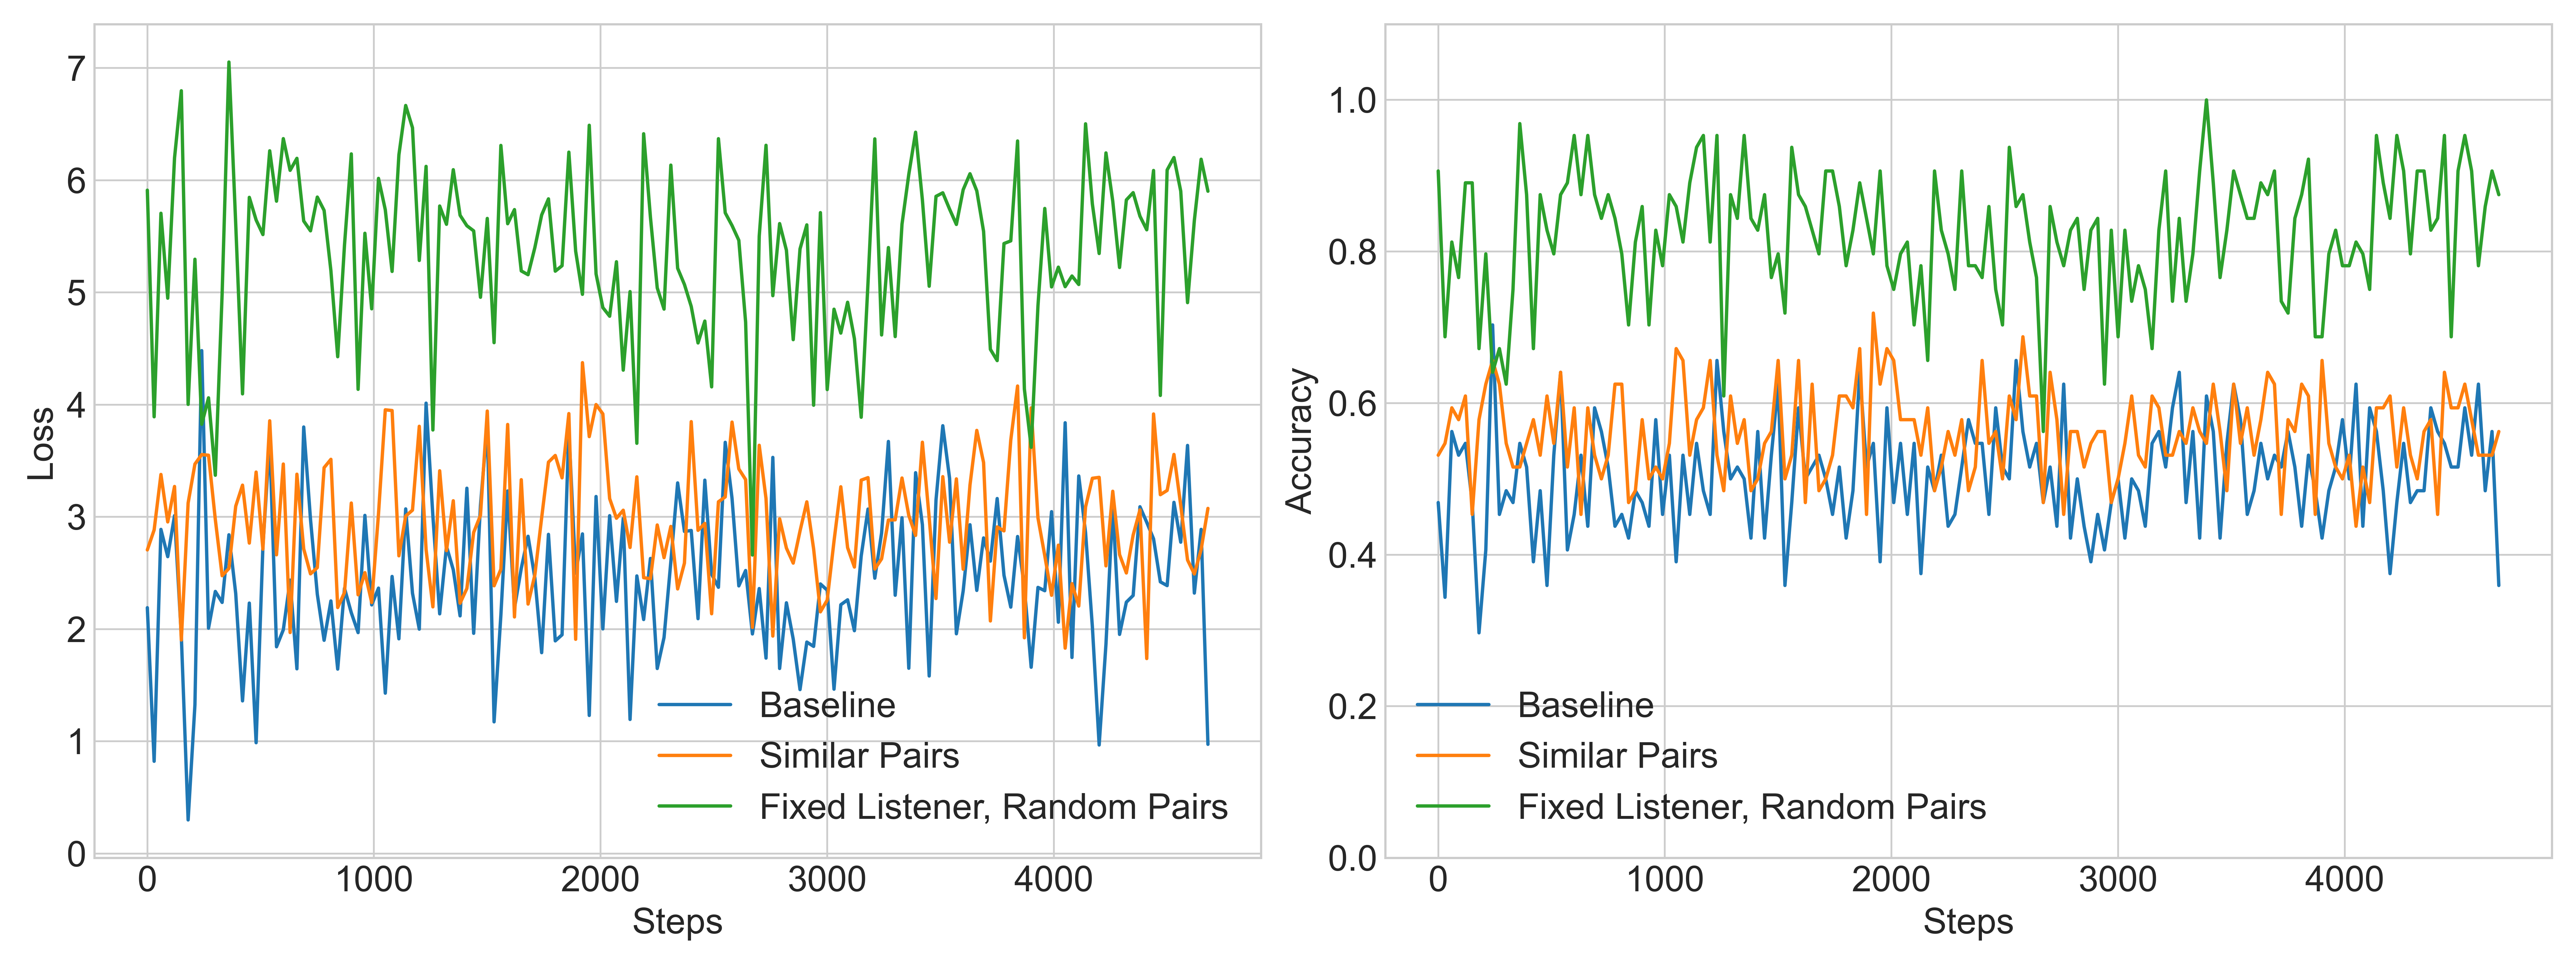
\includegraphics[width=\linewidth]{images/coco_greedy_all_075_losses.png}
	\caption{Training results of three experiment with greedy decoding on MS COCO ($\lambda_s = 0.75$): baseline random pairs, with a fixed listener on random pairs, and with a joint listener on similar pairs. Left: Total speaker training loss. Right: Listener training accuracy.}
	\label{fig:coco_greedy_baseline}
\end{figure} 
Interestingly, although the messages seem to be unsuitable for learning the reference game, their semantic and structural drifts during training were well \emph{above} the drifts of both ground truth captions and the pure decoding experimental results (Fig.~\ref{fig:coco_greedy_drifts}~vs.,~e.g.,~Fig.~\ref{fig:coco_baseline_str_sem_drift_all}). Drift values on the test set clearly indicate that using greedy decoding led to messages with lower structural and semantic drift values. Intuitively, this makes sense because greedy decoding selected the highest probability tokens, resulting in overall higher message probabilities under the pretrained models measuring drift. Even the overlap metrics were higher under greedy test decoding compared to pure test decoding for the random pairs experiments, suggesting that it was not the absence of discriminative words that potentially was responsible for the task failure of the joint listeners. Only for similar pairs greedy decoding might not have been able to retrieve critical discriminative words. This could be because there were less options among which discriminative words could be selected, and these were simply ignored due to lower probability.
\begin{figure}
	\centering
	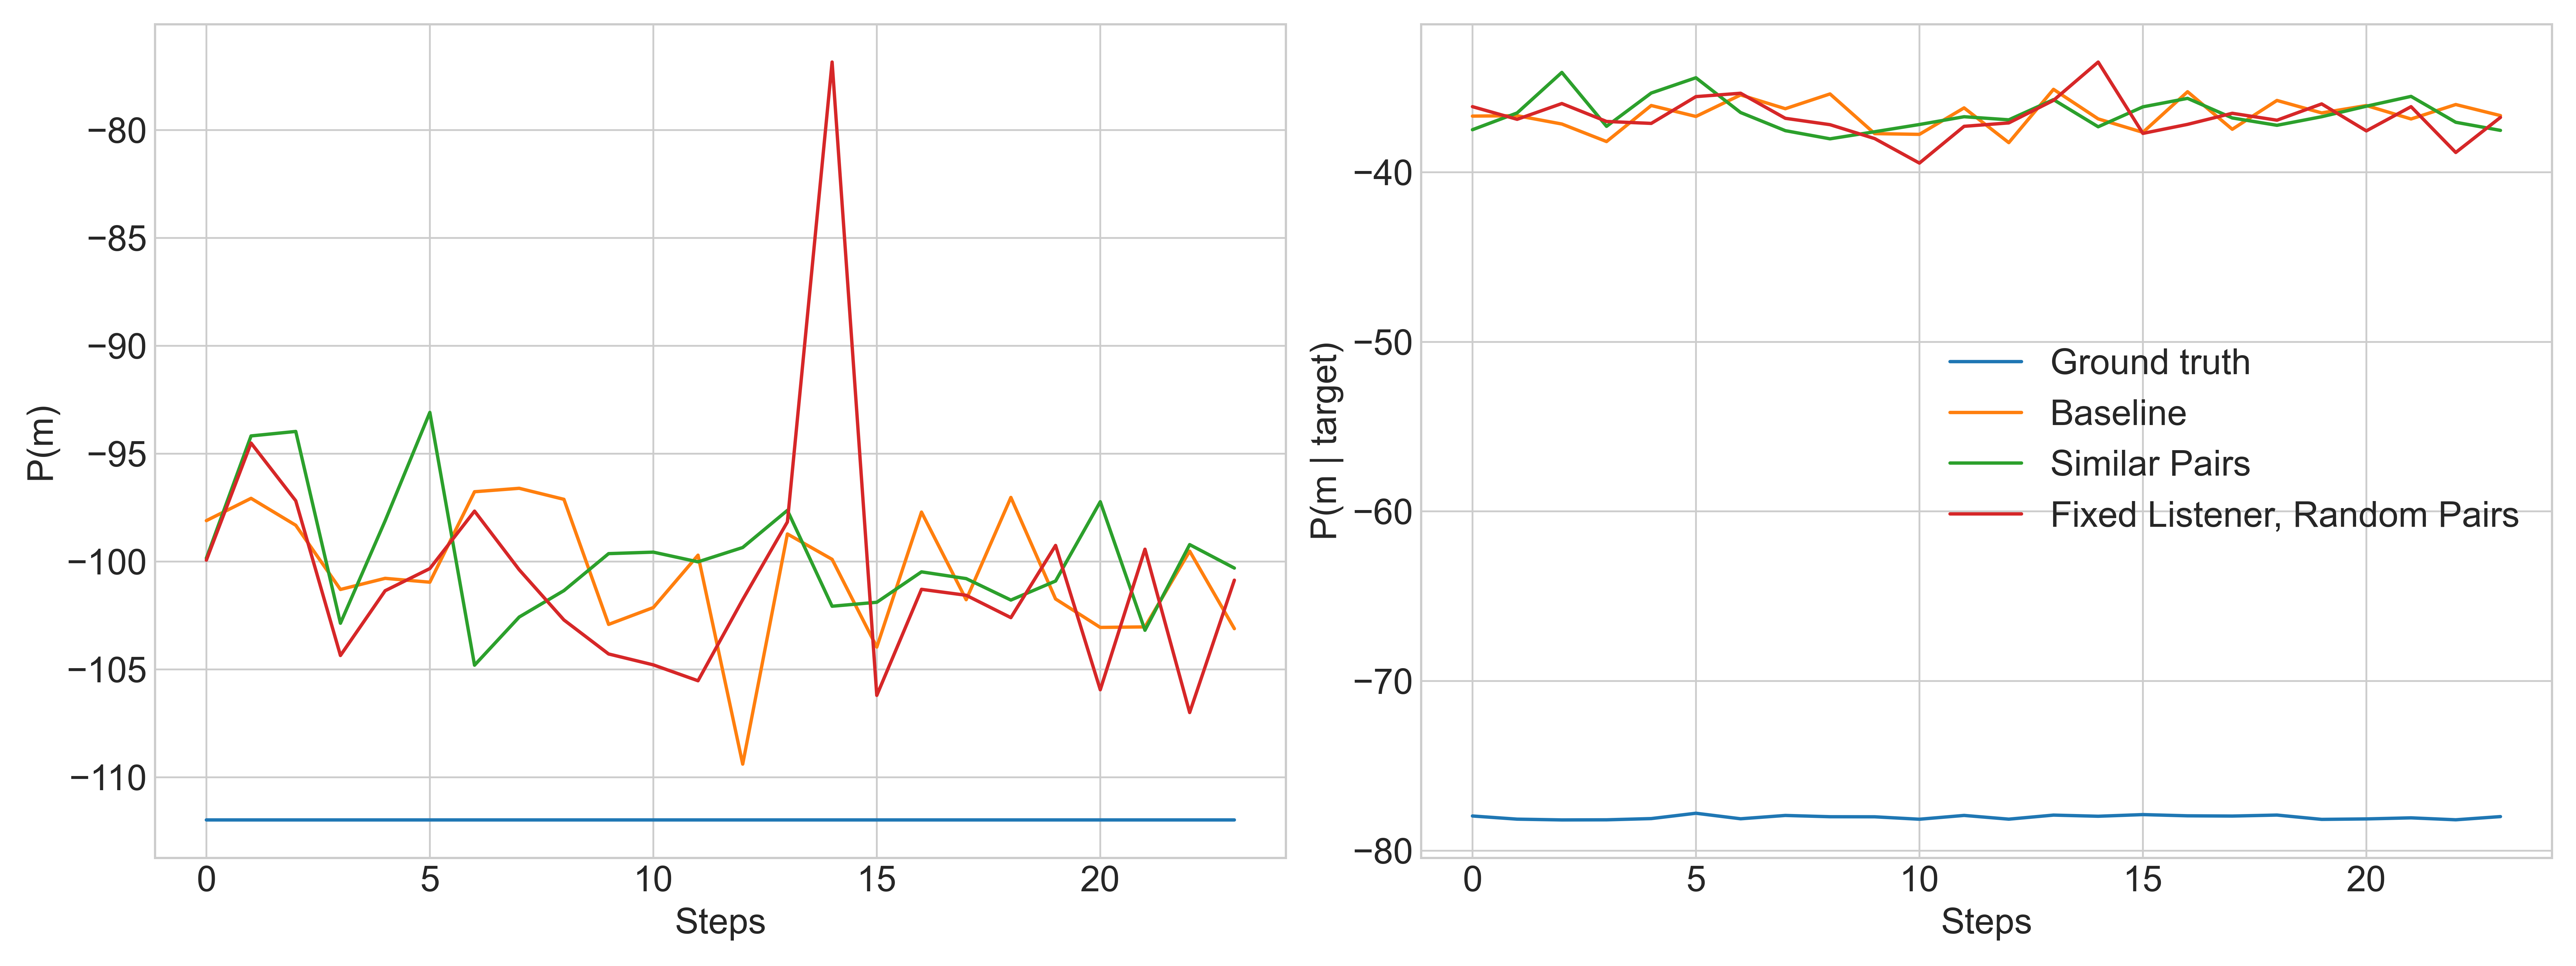
\includegraphics[width=\linewidth]{images/coco_structural_semantic_drift_greedy_all_4000_pure_075.png}
	\caption{Drift computed during training of three MS COCO experimens, using greedy speaker decoding ($\lambda_s = 0.75$). Left: Strucutral drift of ground truth and predicted captions under a pretrained LM. Right: Semantic drift of ground truth and predicted captions under the pretrained speaker model.}
	\label{fig:coco_greedy_drifts}
\end{figure} 

The most plausible explanation for the task failure might be that the speaker was pretrained using pure decoding, yet fine-tuned on the reference game using greedy decoding. This change in strategy might have been disadvantageous for the learned conditioning on the images, hindering the listener from successful grounding. Therefore, for more comprehensive results, these experiments should be replicated using a greedily pretrained speaker. Another potential source of failure might be the observation that greedy decoding agents tend towards word repetitions \parencite[cf.][]{lee2019countering} (see Fig.~\ref{fig:coco_randPairs_speaker_generations}). While the fixed listener might have been able to ignore the repetitions and attend to critical content words, it seems that these repetitions might have overriden the critical grounding signal for the jointly trained listeners. Comparing the fixed listener test semantic drift to the same value in the pure decoding experiment (Tab.~\ref{tab:coco_greedy}~vs.~Tab.~\ref{tab:coco_drift_metrics_basic}), it is visible that the fixed listener did not mitigate semantic drift in the greedy decoding experiment that well, further supporting that greedy decoding fine-tuning might have corrupted the speaker's grounding from pretraining. 
These trends also overpowered differences in the visual input, yielding similar results on random and similar pairs.
Overall, this combination of low drifts with a failure to learn the reference game indicates that the drift values alone are not representative of the agents' success, and factors which are not captured by the metrics may play a critical role for functional success, especially when training the listener agent from scratch. The results also suggest that the decoding strategy is a critical component of the system which may need to be held constant between pretraining and task-based fine-tuning, which may imply limitations when using pretrained models for fine-tuning on downstream tasks.

Summarizing the experiments on the MS COCO dataset, it was shown that artificial agents could learn to play a reference game on real-world images, while using natural language. Their learning speed in the game crucially depended on the discriminability of the target among distractors, which the agents were highly sensitive to. Consistent with the literature, the agents were subject to structural and semantic language drift which was best mitigated by training the speaker against a fixed listener, but, at the same time, was strongly influenced by the quality of the pretrained speaker. The decoding strategy was shown to be an important factor for the drift. Finally, it was shown that task-conditional fine-tuning of the speaker's messages might require longer training, although even a few epochs were sufficient for the speaker to learn a tendency towards adjusting the granularity of her messages according to the complexity of the image pairs.

\subsection{3Dshapes: Baseline Experiments}
\label{expt:3dshapes_baseline}

The goal of these experiments was to investigate the importance of presenting exhaustive example captions to the model during training for potentially mitigating language drift. To this end, the 3Dshapes dataset was annotated with exhaustive captions (see Section \ref{ds:3dshapes}) and various experiments were conducted. %Additionally, these experiments focus on investigating the model's potential to generate informative captions, without being overinformative. \pt{spell out the operationalization}

\begin{table}[] 
	\begin{tabularx}{\textwidth}{|X|l|l|X|X|X|}
		\hline
		\textbf{Model name}                                    & \textbf{log $P(m)$} & \textbf{log $P(m \mid i)$} & \textbf{Overlap (d)} & \textbf{Overlap (c)} & \textbf{Acc.}  \\ \hline
		Ground truth exh.       &      -164.752            &         -101.329               &       6.881             &      0.023               &       0.998 (fixed listener)         \\ \hline
		Pretrained 3D exh. speaker                            &       -195.753            &         -145.638               &        5.428              &      0.001                & 0.920 (fixed listener)            \\ \hline
		3D Baseline, random, $\lambda_s = 0$ &       -195.420            &    -147.938                    &           5.294            &      -0.002                &                 0.979                 \\ \hline
		3D Baseline, random, $\lambda_s = 0.25$     &     -196.811              &       -140.862                 &          5.104            &       -0.006               &          0.969                      \\ \hline
		3D Baseline, random, $\lambda_s = 0.5$   &         -196.722          &        -144.301                &        4.968              &          0.002            &                  0.971            \\ \hline
		3D Baseline, random, $\lambda_s = 0.75$  &       -195.495        &           -147.313           &          5.247            &         0.001             & 0.979               \\ \hline
		3D Baseline, random, $\lambda_s = 1$   &      -196.019             &            -137.456             &        5.257              &          -0.005            &              0.979               \\ \hline
		3D fixed listener, random, $\lambda_s = 0$&      -196.111          &     -136.134                  &             5.339         &         -0.008            &                   0.927              \\ \hline
		3D fixed listener, random, $\lambda_s = 0.75$&      -194.990          &     -140.483                  &             5.298         &         -0.003            &                   0.927             \\ \hline
	\end{tabularx}
	\caption{\label{tab:3dshapes_drift_metrics_basic_baseline} Language drift metrics and listener test accuracies (``Acc.'') on different pairs. 
		``Baseline'' refers to the setup wherein the listener is trained jointly with the speaker, using pure decoding. 3D refers to the 3DShapes dataset. ``Random'' refers to speakers trained on random target-distractor pairs; ``similar'' refers to speakers trained on similar pairs. ``Overlap (d)'' refers to the discrete overlap metric, ``overlap (c)'' to continuous overlap. The speakers trained on similar pairs are still tested on random pairs.}
\end{table}

First, a baseline experiment with pure decoding and $\lambda_s = 0.75$ was conducted.
The configurations as well as the training procedure of this experiment matched the general configurations of the MS COCO baseline experiment in Section \ref{expt:coco_baseline}. The training dynamics of this baseline experiment can be seen in Figure \ref{fig:3dshapes_baseline_speaker_loss_listener_acc_all} (red lines). Interestingly, compared to the reference game on MS COCO (see Fig.~\ref{fig:coco_baseline_speaker_loss_listener_acc_all}, red line), the training of the agents did not visibly converge faster, although the action space (i.e., vocabulary space---49 tokens for 3Dshapes~vs.~4054 tokens for MS COCO) that the speaker had to learn was significantly smaller. 
 
Supporting the visual results, Table \ref{tab:3dshapes_drift_metrics_basic_baseline} shows that the agents successfully learned the reference game---the listener test accuracy was 0.979, even outperforming the MS COCO baseline experiment. Accuracy also improved by 0.026 compared to the pretrained speaker. 
Supporting \textbf{H2}, slight semantic drift can be observed in this experiment---the average conditional log likelihood of the captions generated by the trained speaker decreased by 1.675, compared to the captions produced by the pretrained speaker. In contrast to the MS COCO baseline experiment, \textbf{H1} was not supported in this experiment, as the average log likelihood under the pretrained LM actually increased by 0.258, compared to the pretrained speaker (Table~\ref{tab:3dshapes_drift_metrics_basic_baseline}). Example messages generated by the speaker are showed in Figure~\ref{fig:shapes_randPairs_speaker_generations} (``Baseline speaker exh.'').

\begin{figure}[h]
	\centering
	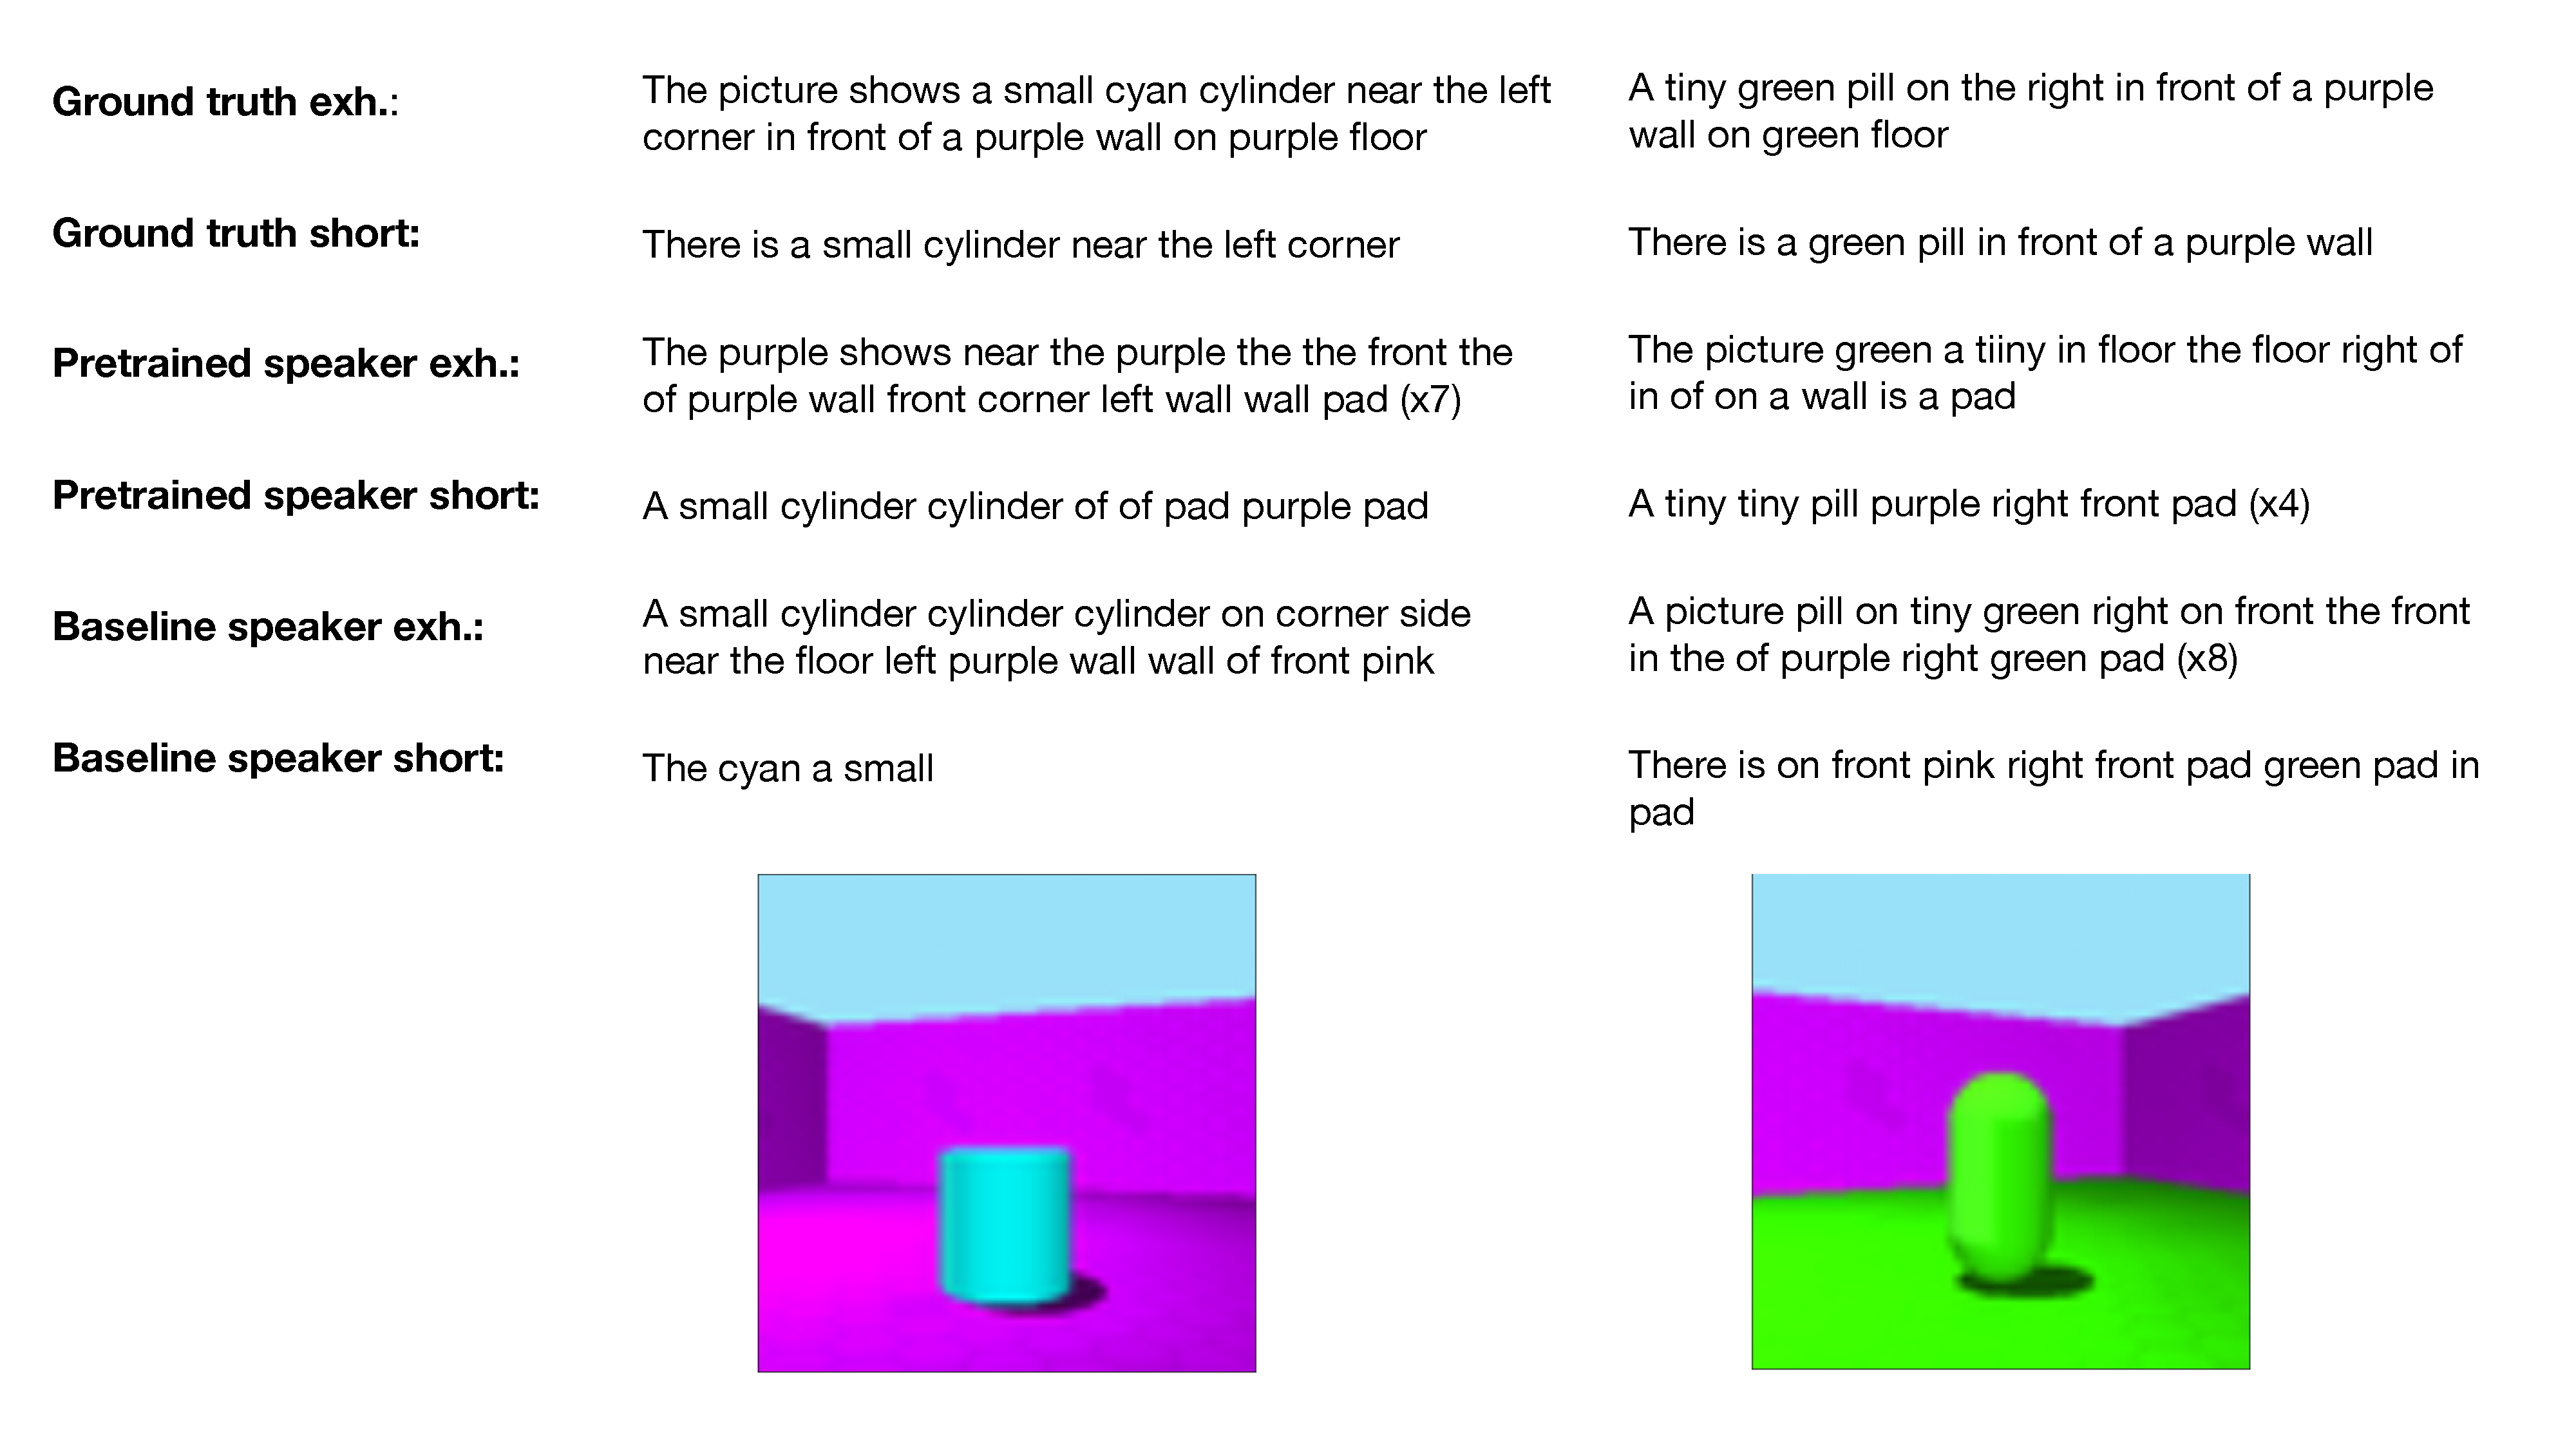
\includegraphics[width=\linewidth]{images/example_generations/shapes_randomPairs.pdf}
	\caption{Examples of messages generate by different speakers. Messages were generated by treating each image as the target in context of the other image as the distractor. Displayed messages are the generations up to the first \texttt{END} token.}
	\label{fig:shapes_randPairs_speaker_generations}
\end{figure}
 
The dynamics of structural and semantic drifts during training can be seen in Figure \ref{fig:3dshapes_baseline_all_str_sem_drift} (red lines); these are in line with the validation results (Tab.~\ref{tab:3dshapes_drift_metrics_basic_baseline}).
Interestingly, the magnitude of the structural drift values was much higher for 3Dshapes than for MS COCO, indicating that the generated captions might in general be less likely under the pretrained Transformer XL model used for the computation. This could be due to the generally lower naturalness of the captions because they describe scenes unlikely to occur in the real world and, therefore, are less likely under a model pretrained on standard natural language corpora. Similarly, the higher magnitude of the semantic drift values indicates that the speaker was generally uncertain when generating captions for these images. This could partly be due to the difference in the 3Dshapes data distribution compared to the ImageNet data on which the visual module of the speaker was pretrained. Additionally, this could be due to the variability of the syntactic structures of the generated ground truth sentences (cf. Section \ref{ds:3dshapes}). 

Turning to the overlap metrics in Table~\ref{tab:3dshapes_drift_metrics_basic_baseline}, against predictions, the discrete overlap decreased by 0.181 tokens on average, compared to the pretrained speaker, while the continuous overlap did not change. Similarly to MS COCO, the overlap was also generally lower than for the ground truth captions, indicating that the trained speaker's captions might not cover all discriminative features mentioned in the exhaustive ground truth captions. An interesting direction for future work is the investigation of potential regularities in the type of feature descriptions omitted by the speaker. A further interesting observation is that the difference in the discrete overlaps between the baseline speaker and the ground truth captions was much smaller in the 3Dshapes experiment (1.634), compared to MS COCO (7.95). This might be an indication of a more robust grounding of the 3Dshapes speaker mentioning more of the features contained in the images, compared to the MS COCO speaker, which might be attributed to the significantly smaller action space of the former. In sum, \textbf{H3} was not supported by the data from the 3Dshapes baseline experiment.

Additionally, the fine-tuned speaker was evaluated with standard image captioning metrics. Table \ref{tab:eval_metrics_refgame} shows that caption quality marginally decreased with respect to almost all metrics except for CIDEr and BLEU-1. Noteworthily, in contrast to the language drift metrics, these metrics are significantly higher for the 3Dshapes dataset compared to MS COCO, indicating that the generated captions have a relatively high overlap with ground truth captions. This calls for careful consideration of the pretraining datasets and their similarity to the target dataset when using available pretrained models like ResNet and Transformer XL.

\subsubsection{Varying Structural Loss}

\begin{figure}[h]
	\centering
	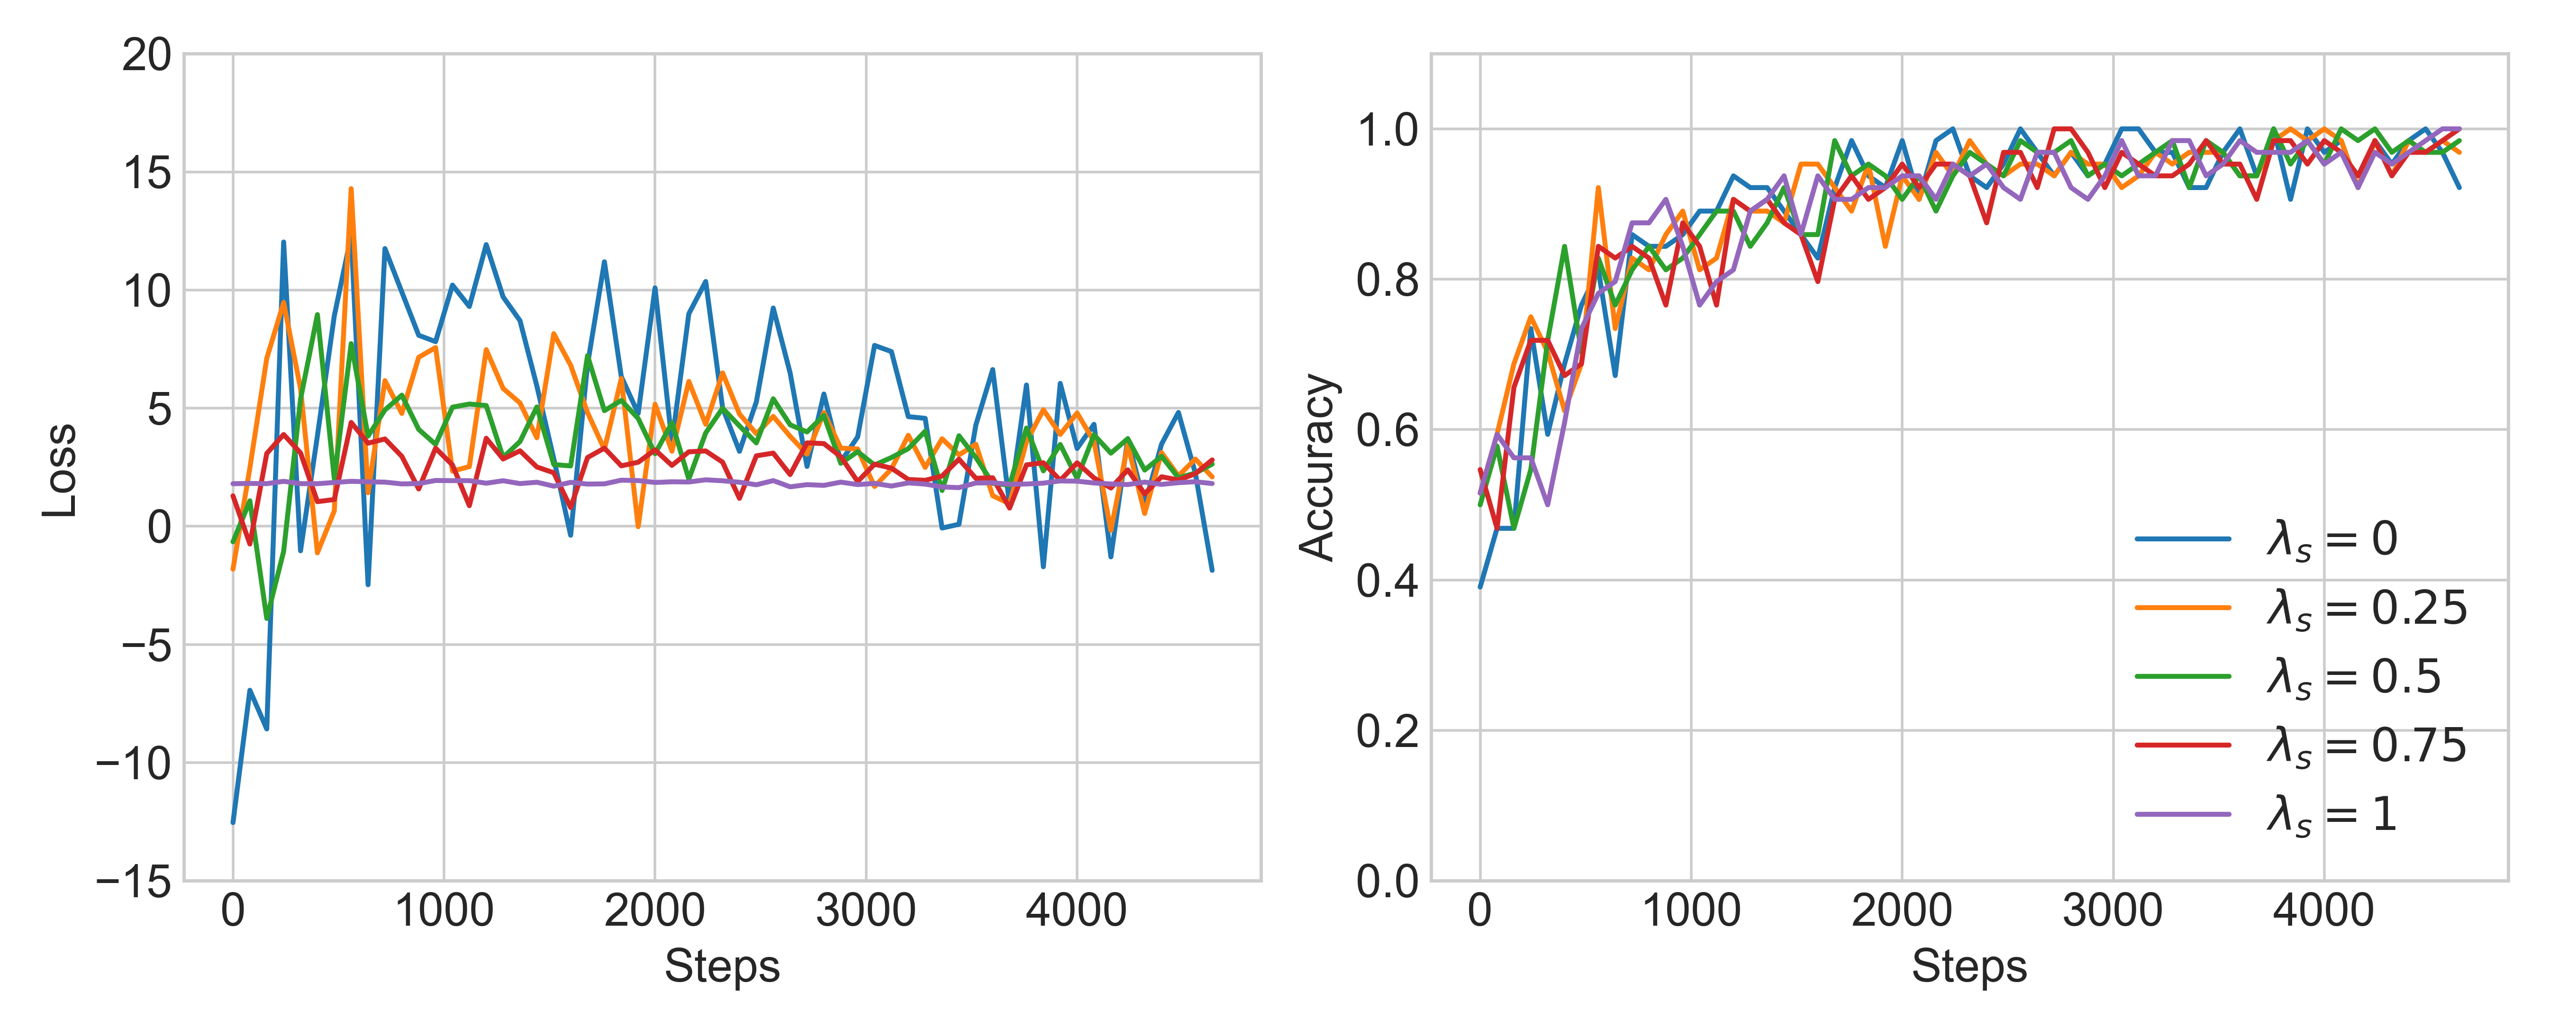
\includegraphics[width=\linewidth]{images/shapes_refgame_49_pure_losses_all_Ls_random.png}
	\caption{Training results of the 3Dshapes experiment with varying $\lambda_s$ weights (pure decoding). Left: Total speaker training loss. Right: Listener training accuracy.}
	\label{fig:3dshapes_baseline_speaker_loss_listener_acc_all}
\end{figure}

\begin{figure}[h]
	\centering
	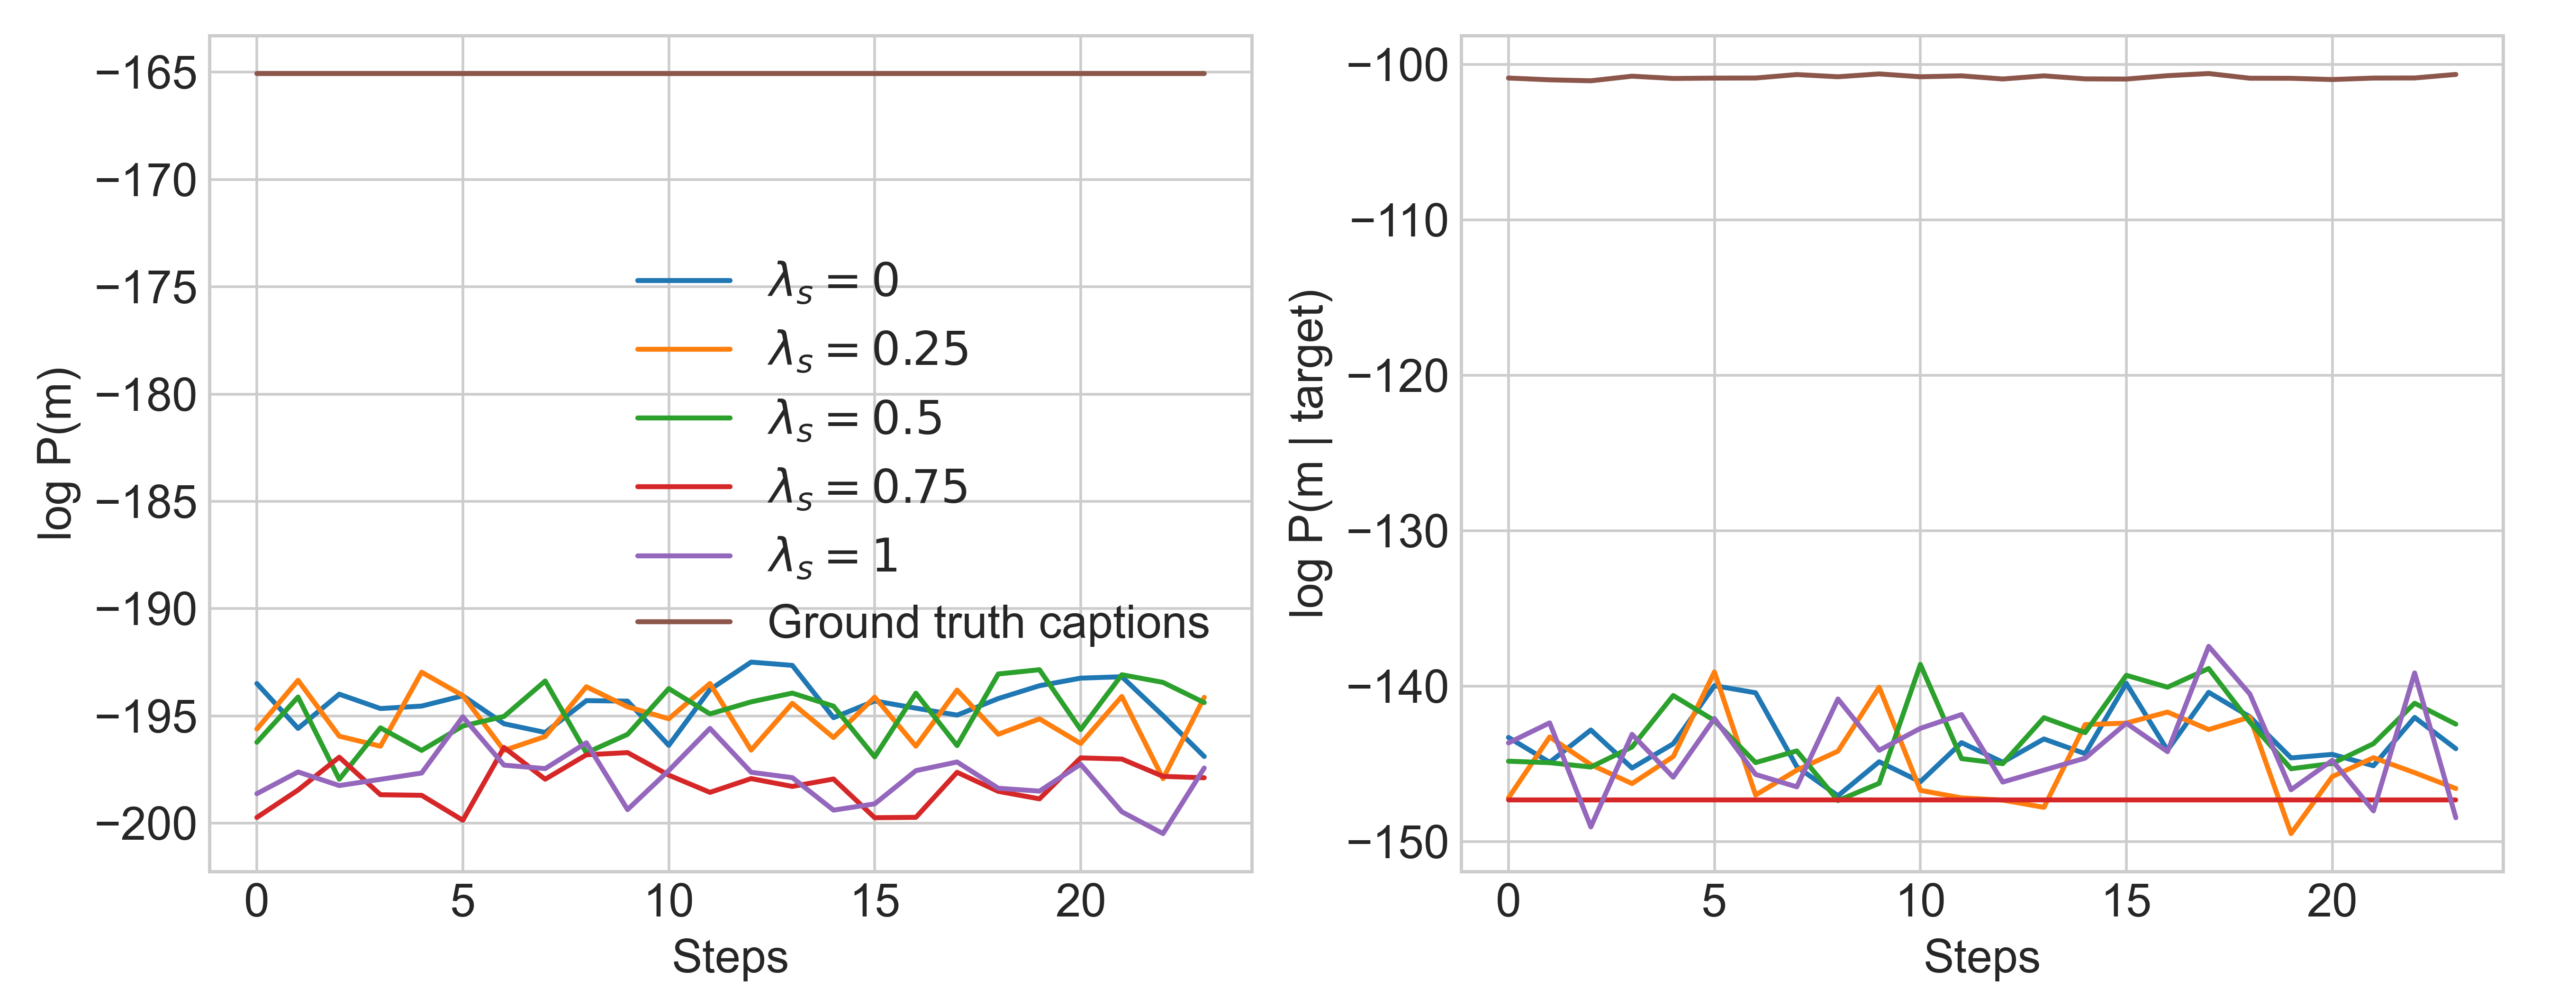
\includegraphics[width=\linewidth]{images/shapes_structural_semantic_drift_49_pure_L_s_all_random.png}
	\caption{Drift metrics computed every 200 training steps on 192 images in the baseline 3Dshapes experiments, across $\lambda_s$ values. Higher values indicate less drift. Left: Strucutral drift of ground truth and predicted captions under a pretrained LM. Right: Semantic drift of ground truth and predicted captions under the pretrained speaker model. The drift is constant for $\lambda_s = 0.75$ due to a coding error, it is instead depicted as the mean validation drift from Table \ref{tab:3dshapes_drift_metrics_basic_baseline}.} 
	\label{fig:3dshapes_baseline_all_str_sem_drift}
\end{figure}

In order to address \textbf{H4} with the 3Dshapes dataset, a line of experiments identical to MS COCO ones was conducted. Specifically, the structural loss weight $\lambda_s$ was also varied. The pattern of results visible in Figure~\ref{fig:3dshapes_baseline_speaker_loss_listener_acc_all} was very similar to MS COCO. The magnitude of the speaker loss is what was mostly influenced by the $\lambda_s$ weight; the listener's training accuracy was not affected by the variation. This is confirmed by the consistently high listener test accuracy, outperforming the pretrained speaker (Table~\ref{tab:3dshapes_drift_metrics_basic_baseline}, fifth column).% Differently to MS COCO, the speaker trained with $\lambda_s = 1$ outperformed the pretrained speaker by 0.026, indicating that there might have been room for further improving the speaker's structural skills.

Also following the general procedure, validation language drift metrics on 3Dshapes were computed on a held out test set of 1000 images. Table \ref{tab:3dshapes_drift_metrics_basic_baseline} indicates that, similarly to MS COCO, no clear trends can be observed with respect to all four drift metrics. Negative continuous overlap values (Tab.~\ref{tab:3dshapes_drift_metrics_basic_baseline}, fourth column) indicated that the emebddings of generated captions were partly more similar to the distractor ground truth embeddings, than to target ground truth embeddings. These findings were generally corroborated by the dynamics of structural and semantic drifts computed during training (see Fig.~\ref{fig:3dshapes_baseline_all_str_sem_drift}). In contrast to MS COCO, semantic drift of the captions produced by the speakers was stronger than of the ground truth captions, i.e., the conditional log likelihood of the generated captions was lower. 

These experiments in comparison to analogous experiments on MS COCO (Section \ref{expt:coco_baseline}) also allowed to adress \textbf{H7} as they provided different degrees of freedom for the model to exploit structural deterioration as a method for producing more discrminative captions. In line with \textbf{H7}, the largest difference in structural drift compared to the pretrained speaker in 3Dshapes experiments on random image pairs was 1.058 (Tab.~\ref{tab:3dshapes_drift_metrics_basic_baseline}), compared to 5.164 on MS COCO (Tab.~\ref{tab:coco_drift_metrics_basic}). That is, these results supported \textbf{H7}.

To sum up, similarly to MS COCO, the precise parametrization of the loss did not consistently influence task performance or language drift, given the model and the dataset, indicating that there was no connection to the presence of exhaustive annotation examples in the training dataset when it came to the strength of structural contraints put on the speaker.

\subsection{3Dshapes: Similar Pairs Experiments}
\label{expt:3dsapes_similar}

\begin{table}[]
	\begin{tabularx}{\textwidth}{|X|l|l|X|X|X|}
		\hline
		\textbf{Model name}                                    & \textbf{log $P(m)$} & \textbf{log $P(m \mid i)$} & \textbf{Overlap (d)} & \textbf{Overlap (c)} & \textbf{Acc.} \\ \hline
		Ground truth exh.       &      -164.752            &         -101.329               &       6.881             &      0.023               &       0.998 (fixed listener)       \\ \hline
		Pretrained 3D exh. speaker                            &       -195.753            &         -145.638               &        5.428              &      0.001                & 0.920 (fixed listener)         \\ \hline
		3D Baseline, random, $\lambda_s = 0.75$  &       -195.495        &           -147.313           &          5.247            &         0.001             & 0.979               \\ \hline
		3D Baseline, similar, $\lambda_s = 0.75$ &      -198.189             &       -140.786                 &           5.578           &        0.001              &         0.906                        \\ \hline
		%3D Baseline, similar fixed, random test &       -193.709            &    -141.010                  &        3.280            &      -0.003         &            0.688           \\ \hline
		3D Baseline, similar fixed, same test &      -199.014        &        -146.280           &        2.875       &      0.029   &     0.691                   \\ \hline
		3D Baseline, similar fixed, diff. test &     -194.510     &    -146.557          &   2.071      & 0.020    &     0.570          \\ \hline
		%3D Short, similar, $\lambda_s = 0.75$&      -145.014             &      -76.474                  &             1.565         &         0.000             &                   0.885                       &                                           \\ \hline
		%3D Short, similar fixed, same test $\lambda_s = 0.75$&      -190.010           &     -58.128                  &             2.086         &         0.001             &                   0.731                       &                                           \\ \hline
		%3D Short, similar fixed, diff. test $\lambda_s = 0.75$&     -191.051        &        -59.088           &   1.947        &        0.002          &        0.717                               &                                           \\ \hline
		3D fixed listener, similar fixed, same test &  -198.434       &      -147.121     &     2.892 &    0.025 &      0.744      \\ \hline
		3D fixed listener, similar fixed, diff. test & -198.188   & -143.309      & 2.187   & 0.045    & 0.822     \\ \hline
	\end{tabularx}
	\caption{\label{tab:3dshapes_drift_metrics_basic_similar} Language drift metrics and listener test accuracies (``Acc.'') on varying pairs. 
		``Baseline'' refers to the setup wherein the listener is trained jointly with the speaker, using pure decoding. ``Random'' refers to speakers trained on random target-distractor pairs; ``similar'' refers to speakers trained on similar pairs, ``similar fixed'' being the experiments where the image pairs matched on three fixed features. ``Overlap (d)'' refers to the discrete overlap metric, ``overlap (c)'' to continuous overlap. ``Random'' test refers to random held out image pairs, ``same / diff.'' to pairs matching on the same and different features, respectively.}
\end{table}

\begin{figure}[h]
	\centering
	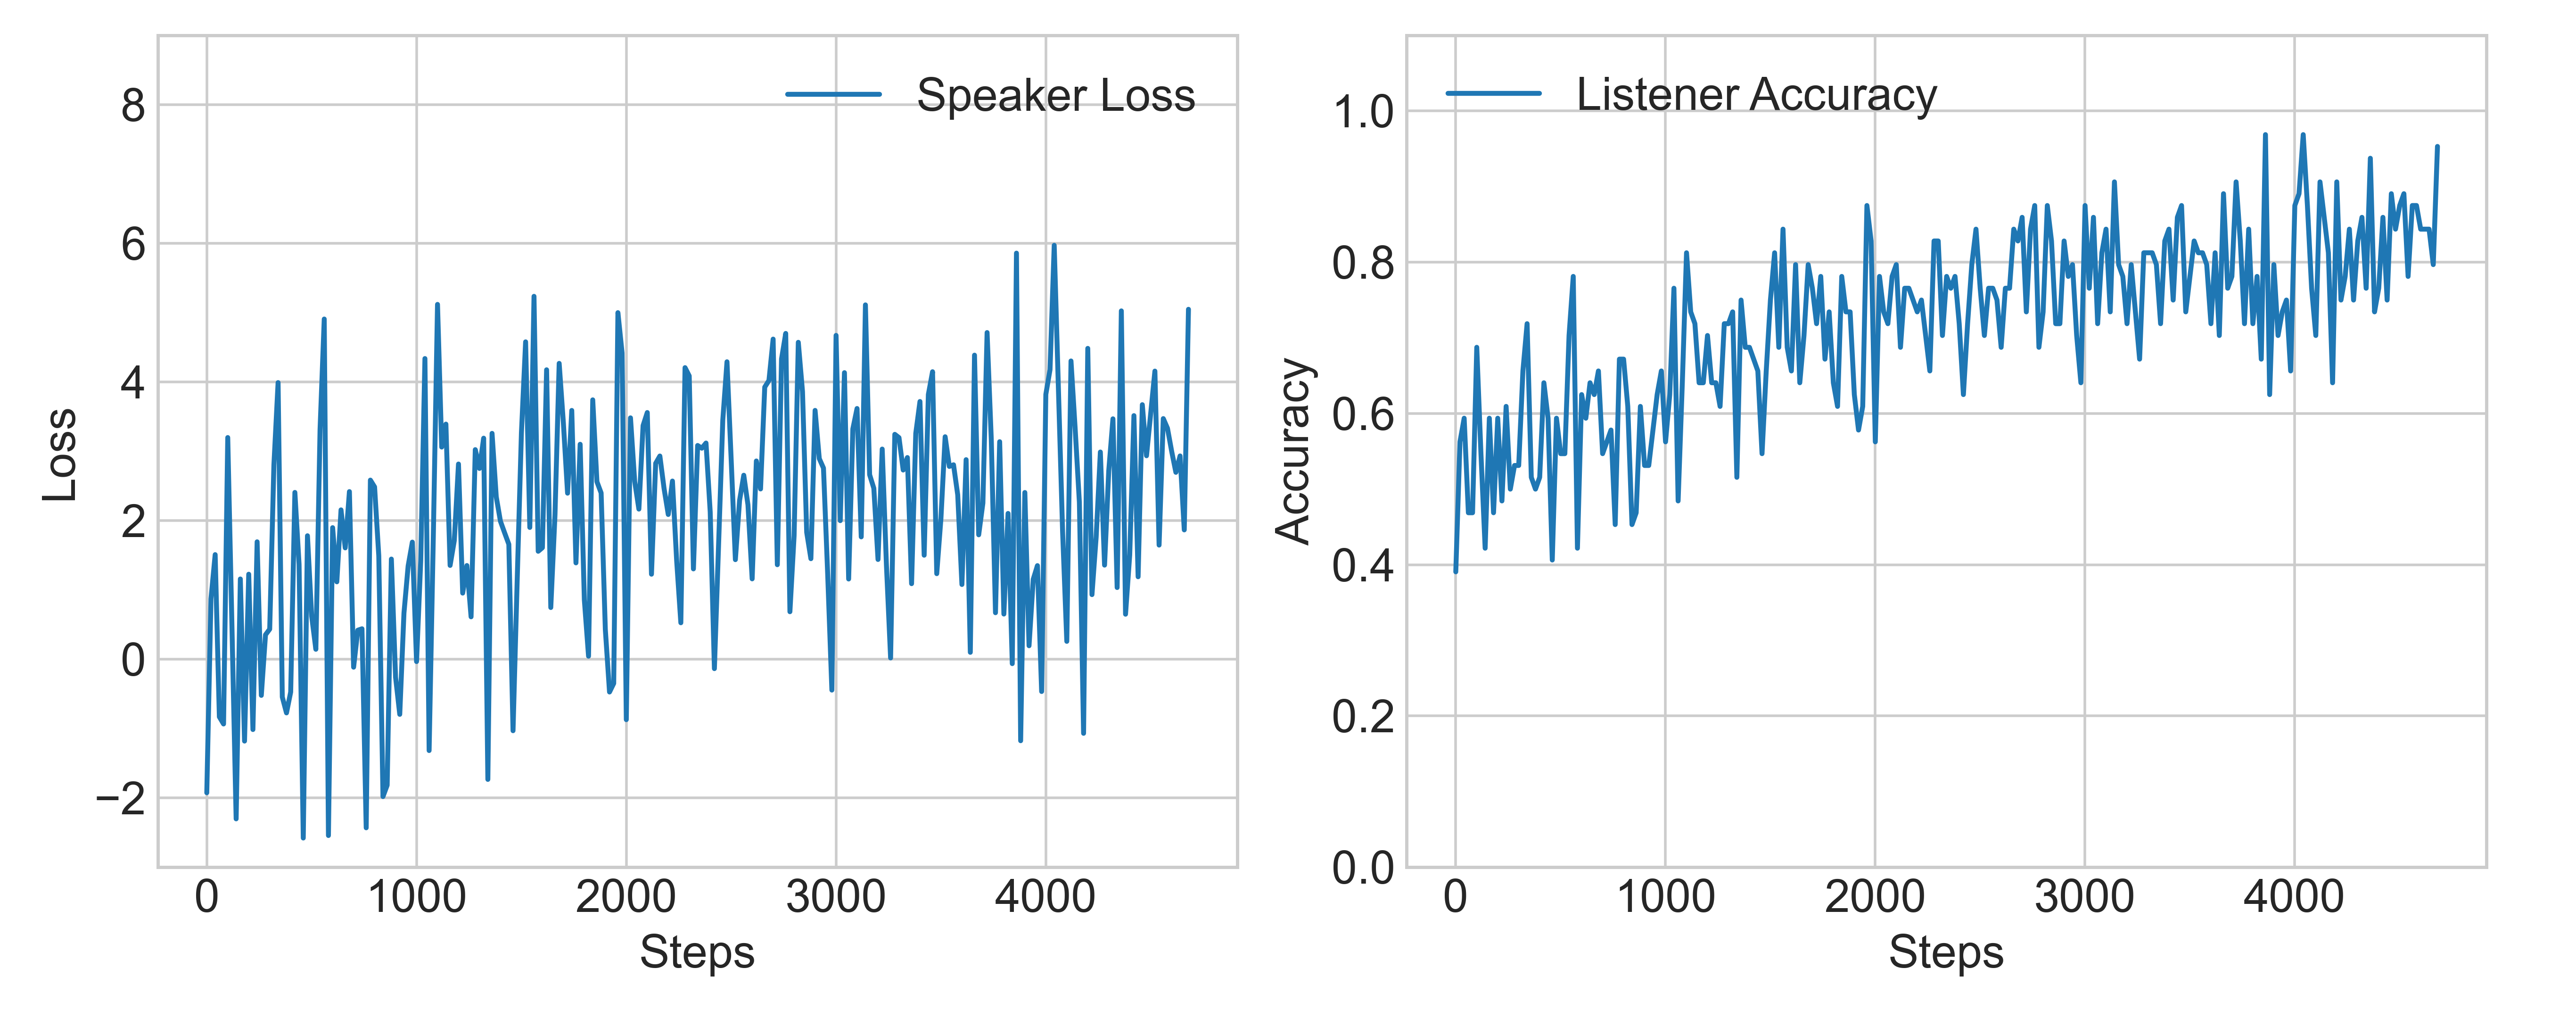
\includegraphics[width=\linewidth]{images/3dshapes_refgame_49_pure_075_similar.png}
	\caption{Training results of the 3Dshapes experiment on similar image pairs (pure decoding, $L_s = 0.75$). Left: Total speaker train loss. Right: Listener train accuracy.}
	\label{fig:3dshapes_similar_075_speaker_loss_listener_acc}
\end{figure}

\begin{figure}[h]
	\centering
	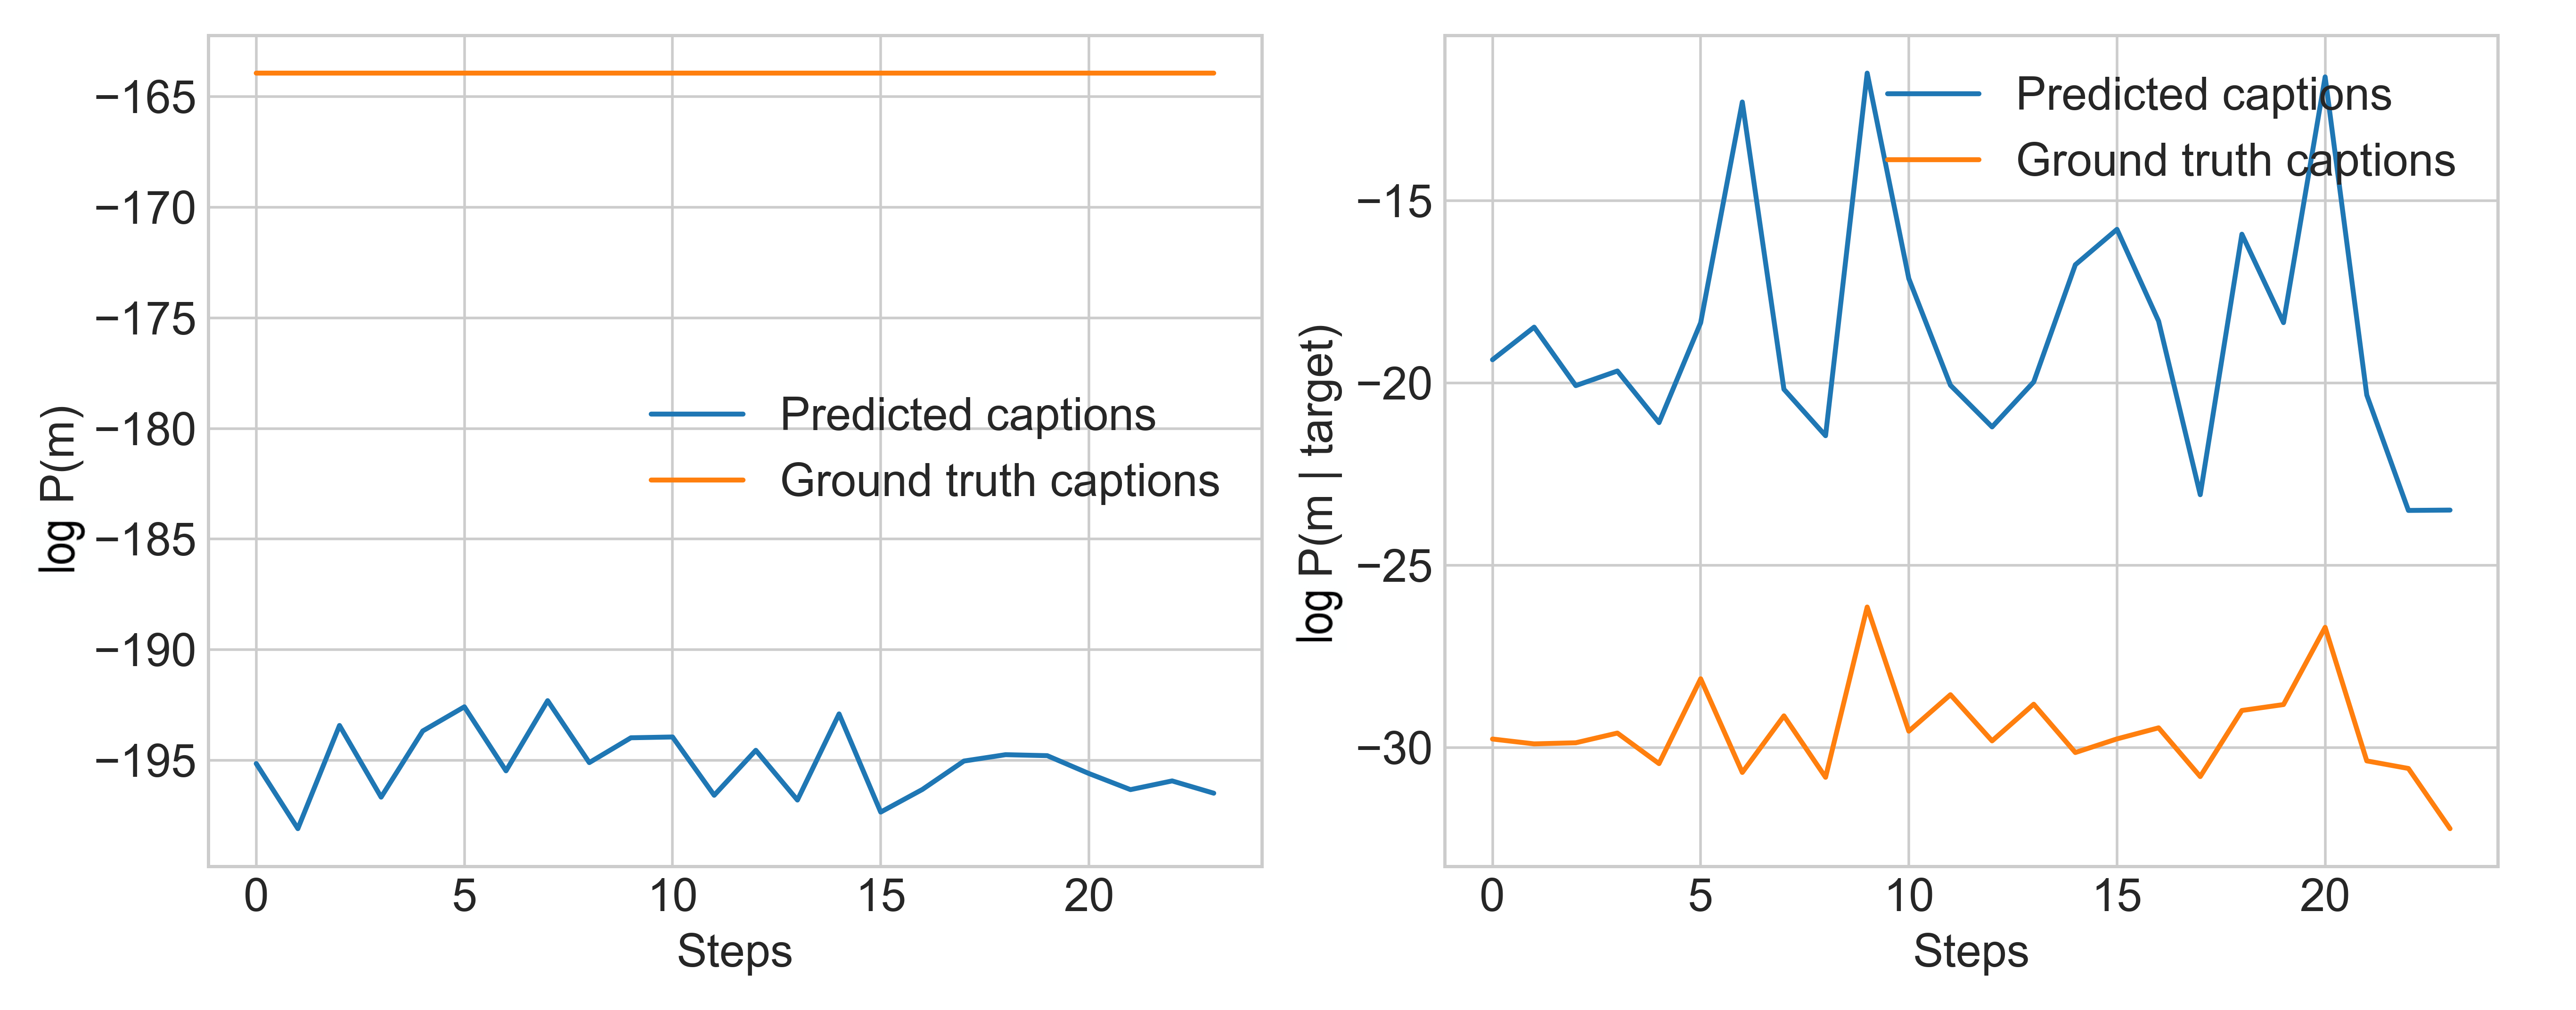
\includegraphics[width=\linewidth]{images/3dshapes_structural_semantic_drift_4000_pure_075_similar.png}
	\caption{Drift values computed during training in the similar image pairs of the 3Dshapes experiment (pure decoding, $L_s = 0.75$, pairs constructed with any features). Higher values are better. Left: Structural drift of ground truth and predicted captions. Right: Semantic drift of ground truth and predicted captions under the model pretrained on similar image pairs.} 
	\label{fig:3dshapes_similar_075_str_sem_drift}
\end{figure}

In this experiment, the target-distractor pairs consisted of similar images. That is, at least three of the six features selected at random matched in the target and distractor image. Otherwise, the procedure and configurations were the same as in the baseline experiment in Section \ref{expt:3dshapes_baseline}. 
Figure \ref{fig:3dshapes_similar_075_speaker_loss_listener_acc} (left) indicates that it was much harder for the speaker to learn producing discriminative messages when the target-distractor pairs were similar, compared to random pairs (Fig.~\ref{fig:3dshapes_baseline_speaker_loss_listener_acc_all}, red lines). There were less options for producing discriminative messages, such that the functional training signal was much weaker than in the former experiment. The listener was much slower to learn the reference game and the grounding of the speaker's messages in the images, respectively (Figure \ref{fig:3dshapes_similar_075_speaker_loss_listener_acc}, right). These dynamics confirm that the agents were sensitive to their visual input, and that the task success was closely dependent on the perceptual difficulty to discriminate the target and distractors. These results pattern with the similar pairs experiment on MS COCO (Section \ref{expt:coco_similar_pairs}), although the 3Dshapes agents were faster to learn the reference game on similar pairs. Nonetheless, the agents were still able to learn the reference game successfully, as indicated by rather high test accuracy (Tab.~\ref{tab:3dshapes_drift_metrics_basic_similar}, ``3D Baseline, similar, $\lambda_s = 0.75$'')

The main hypothesis addressed in this experiment was whether the agents were able to flexibly adapt the specificity of their messages, compared to the random pairs baseline experiment (\textbf{H5}). This was approximately investigated via the distribution of POS tags in messaged generated for a test set of 1,000 target-distractor pairs.\footnote{The term POS tagging is used in a rather loose sense here---the tags were created manually such that they reflected the specific feature of the image the respective word is used in reference to for this dataset.} The distributions were compared when the 1,000 pairs were random versus similar. The results are shown in Figure \ref{fig:3dshapes_pos}. Based on visual inspection, it can be seen that the distribution of the token categories, especially the modifier tokens like color or size adjectives, did not shift significantly depending on the type of pairs (blue~vs.~orange), neither for the random nor the similar pairs experiment speaker. This suggests that the speaker agent was not as flexible in adapting the granularity of feature descriptions in her messages to differences in the input as human speakers (cf. Chapter \ref{chapter03}). Furthermore, there was no apparent difference between speakers trained on the different types of pairs, indicating that the considered training on similar pairs did not lead to better speaker adaptation to more complex visual input. However, it is evident from Figure \ref{fig:3dshapes_similar_075_speaker_loss_listener_acc} that the agents did not converge after two epochs, so longer training might provide a different picture.

\begin{figure}[h]
	\centering
	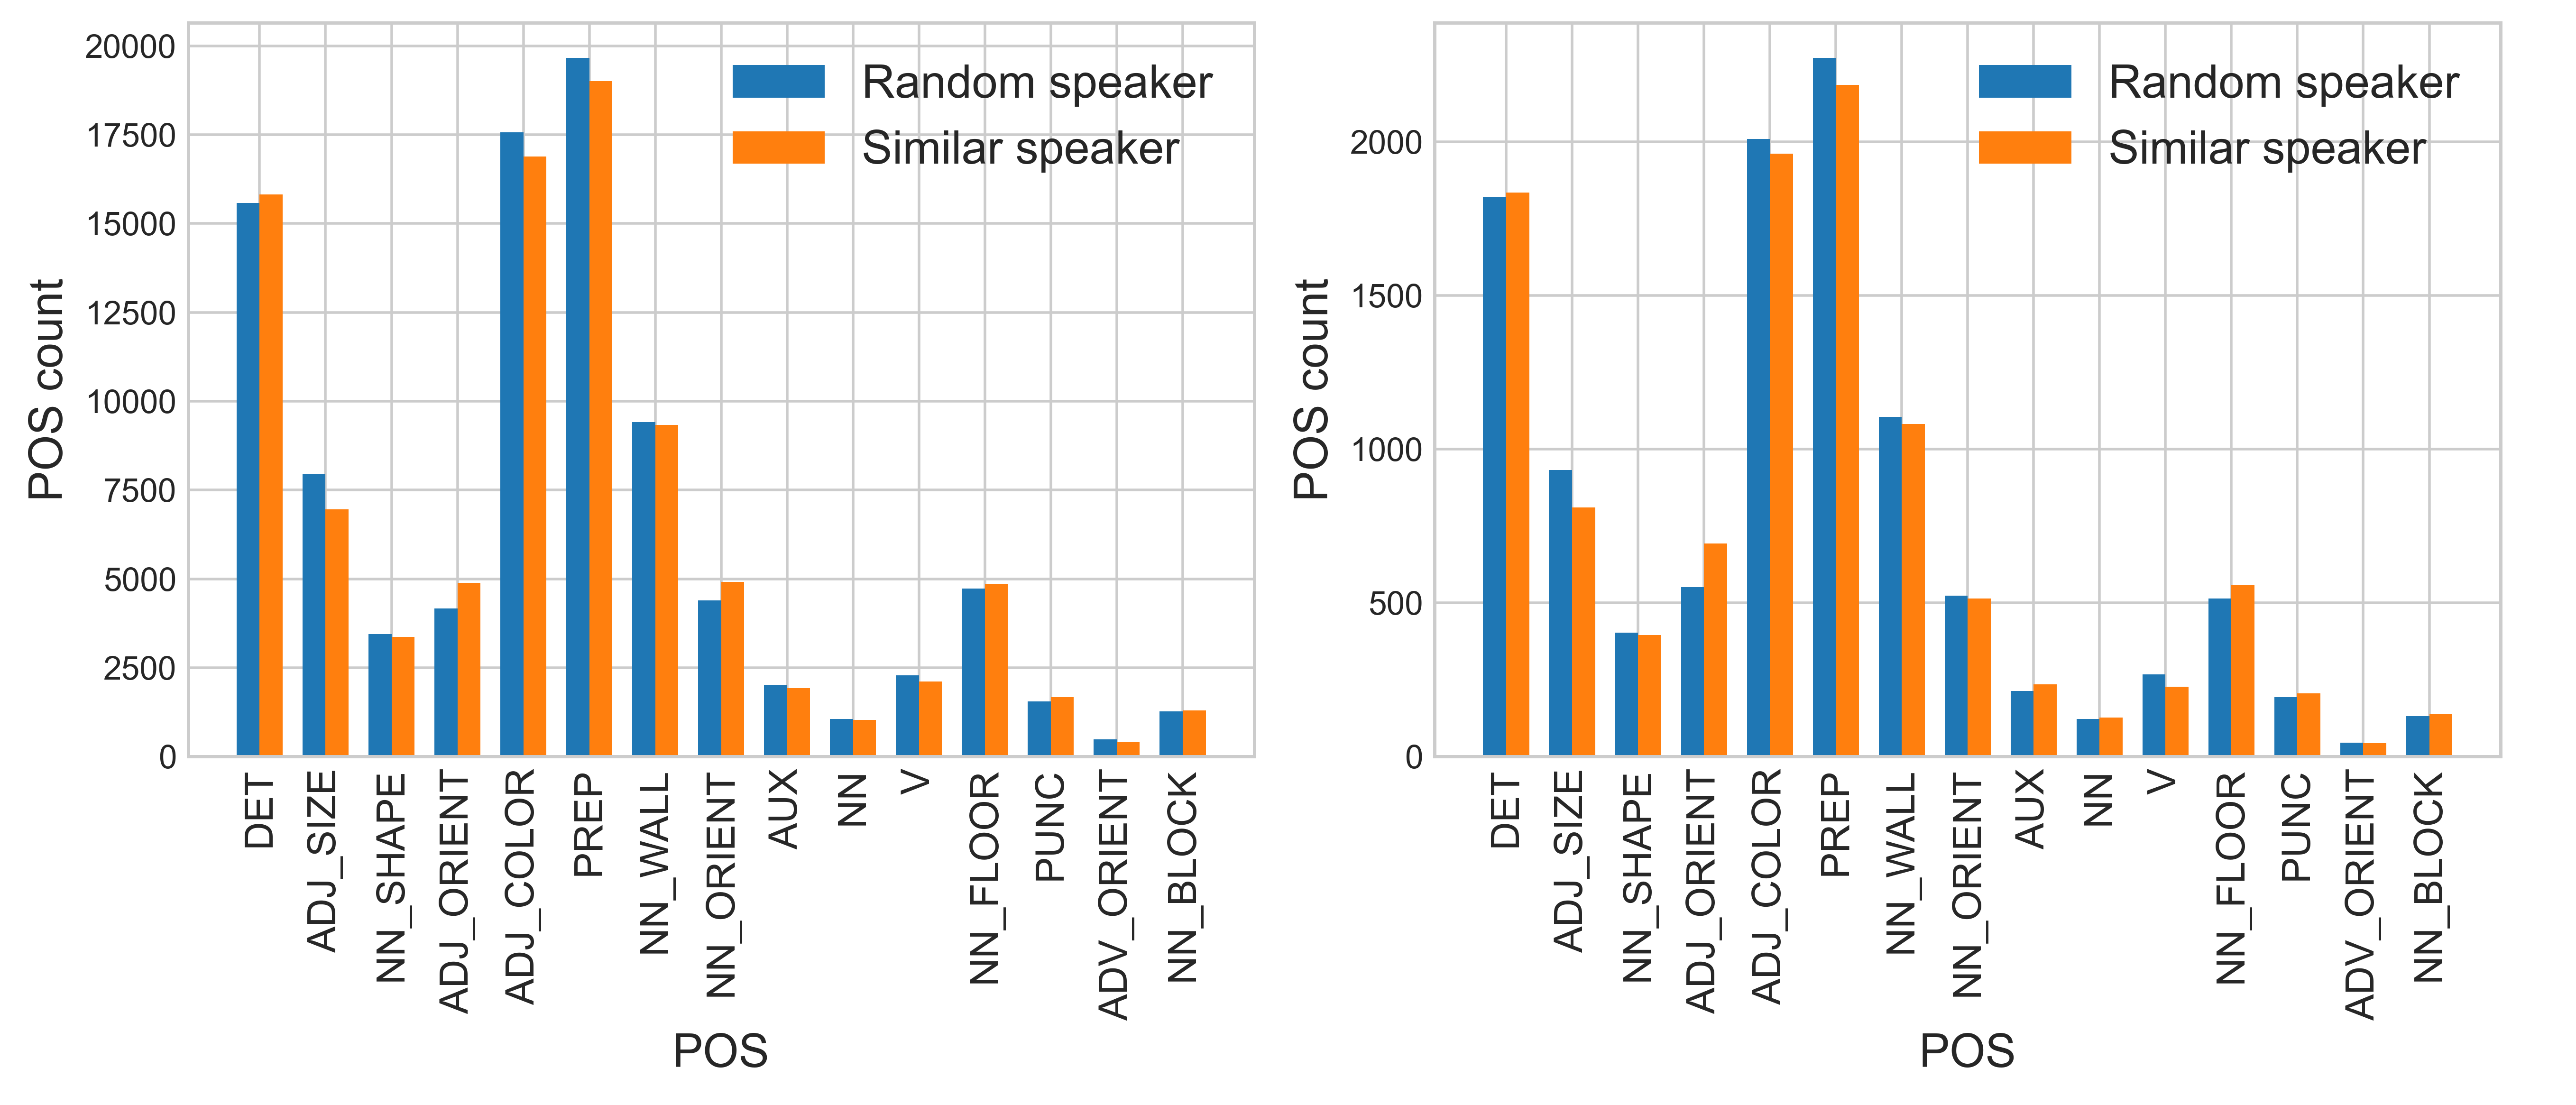
\includegraphics[width=\linewidth]{images/3dshapes_random_vs_similar_POS_counts.png}
	\caption{Left: POS counts in captions produced by a speaker trained on random pairs (blue) and a speaker trained on similar pairs (orange) for 1000 random test image pairs. Right: POS counts in captions produced by a speaker trained on random pairs (blue) and a speaker trained on similar pairs (orange) for 100 similar test image pairs. \pt{The difference in the number of pairs will be fixed}}
	\label{fig:3dshapes_pos}
\end{figure}

In this experiment, stronger structural drift compared to both the pretrained speaker and the baseline experiment could be observed (see Table \ref{tab:3dshapes_drift_metrics_basic_similar}), which was corroborated by a slight visually apparent trend in Figure \ref{fig:3dshapes_similar_075_str_sem_drift}.\footnote{Due to a coding mistake 50 images from the training dataset were used for the computation. Greedy decoding for semantic drift was employed, and the values were computed using one image pair only.} Again patterning with MS COCO results, semantic drift was lower for the similar pairs compared to the random pairs experiment. Going beyond MS COCO, the drift was even smaller than for the pretrained speaker (Tab.~\ref{tab:3dshapes_drift_metrics_basic_similar}). This suggests that the reference game signal helped fine-tuning the speaker.
A little increase in the discrete overlap compared to the pretrained speaker and to the random pairs baseline indicated that the speaker improved on the task and found a way of producing slightly more discriminative messages (Tab.~\ref{tab:3dshapes_drift_metrics_basic_similar}), inspite of perceptual similarity of the images. In sum, these similar pairs experiment results on 3Dshapes did not provide evidence in support of \textbf{H5}. One reason for this might be the variability in the features the images matched on and the potentially varying difficulty for a model to discriminate them. For instance, fine-grained object size differences might be more difficult to detect compated to different object types.

The speaker was also evaluated with image captioning metrics; results in Table \ref{tab:eval_metrics_refgame} show that caption quality almost did not change on any metrics, compared to the pretrained speaker and the random pairs baseline. This stands in contrast to the agents' lower task accuracy and to the MS COCO result. This could be attributed to the fact that these metrics are usually applied to corpora with larger voabularies than 49 tokens, such that behavior on such a dataset might be unexpected.

In order to investigate effects of visual pair similarity in more detail, a follow-up experiment was conducted wherein the features along which the target and the distractor matched were fixed. These features were the object type (cube, ball, pill or cylinder), the object color and the background color (see Fig.~\ref{fig:shapes_similarPairs_example_generations} for an example).
The selection of these features for being fixed was rather arbitrary, and follow-up experiments should address the visual discriminability of different features more systematically. The training results can be seen in Figure~\ref{fig:3dshapes_wShort_similarFixed_075_speaker_losses_listener_acc} (blue lines). Visually, the agents' task performance did not differ much from the random pairs experiments (Fig. \ref{fig:3dshapes_baseline_speaker_loss_listener_acc_all}, red lines). Yet compared to the previous experiment wherein all fixed features were considered, the agents learned the reference game more quickly (Fig.~\ref{fig:3dshapes_similar_075_speaker_loss_listener_acc}). In order to investigate the listener's test accuracy as well as details of language drift, two kinds of evaluations were done. First, the agents were tested on a held out test set of 1,000 similar image pairs which matched along the same features as the pairs used during training (\textit{same features} test). Second, they were tested on a held out test set of 1,000 image pairs which matched along the \emph{other three} features than the training pairs (i.e., floor color, size of the object and its position in the room, \textit{different features} test). The motivation for this distinction was to investigate whether the speaker was capable to adjust the granularity of her messages depending on the familiarity of the distinctive features.

\begin{figure}[h]
	\centering
	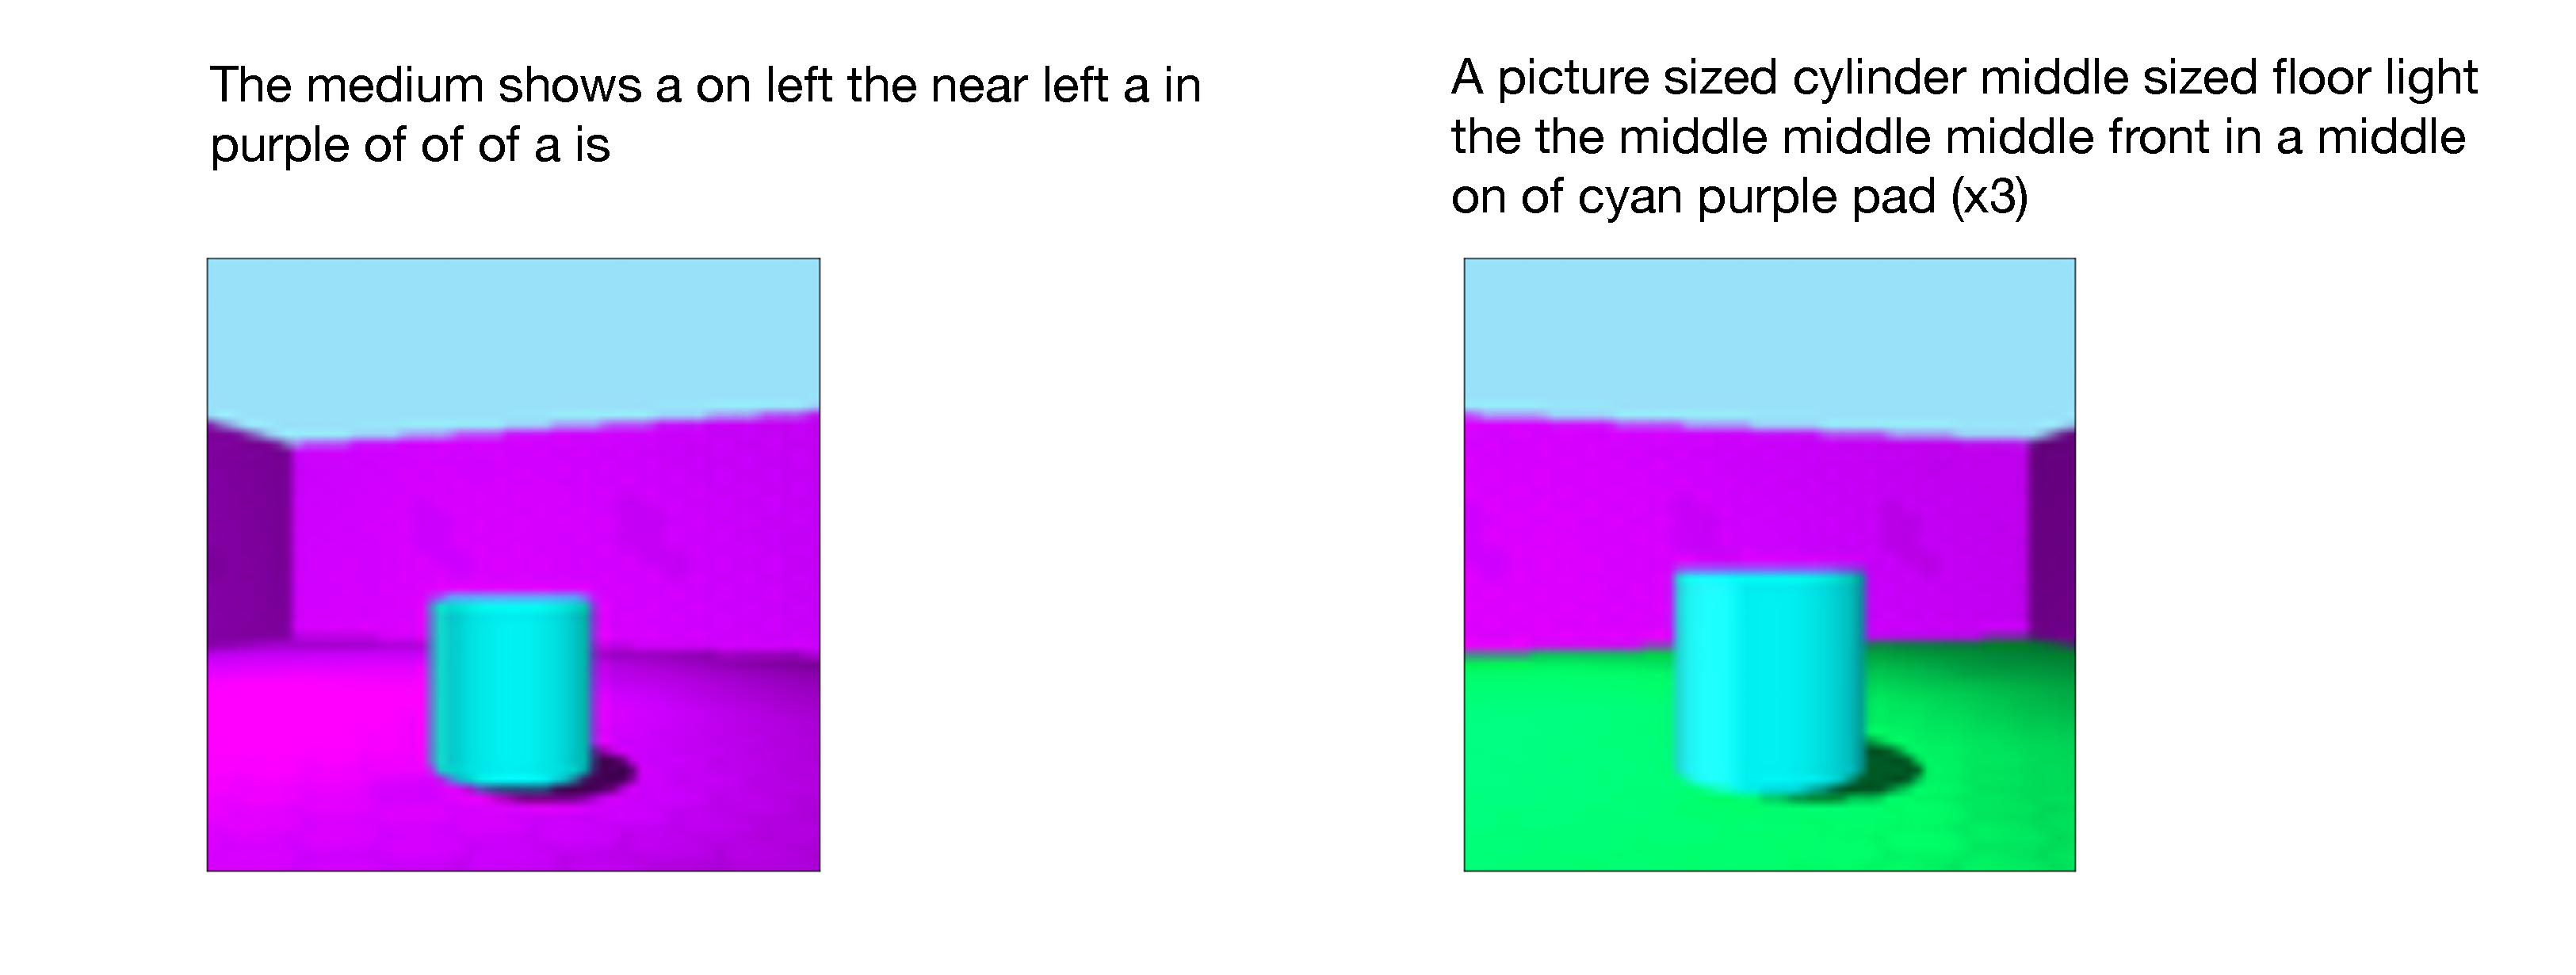
\includegraphics[width=0.9\linewidth]{images/example_generations/shapes_similarPair_cropped.pdf}
	\caption{Examples of messages generate by the speaker trained on similar pairs (matched on fixed features). Messages were generated by treating each image as the target in context of the other image as the distractor. Displayed messages are the generations up to the first \texttt{END} token}
	\label{fig:shapes_similarPairs_example_generations}
\end{figure}
The listener test accuracy of 0.691 (Table \ref{tab:3dshapes_drift_metrics_basic_short}) on the same features test set was surprisingly low compared to the training accuracy (Fig. \ref{fig:3dshapes_wShort_similarFixed_075_speaker_losses_listener_acc}, right, blue line), hinting at potential speaker-listener co-adaptation and overfitting on the training set. The test accuracy on different features was even lower (0.570), confirming that it was more difficult for the agents to communicate about unfamiliar distinctive features. An example speaker message for a similar pair matched on same features can be seen in Figure~\ref{fig:shapes_similarPairs_example_generations}.

The language drift dynamics shown in Figure \ref{fig:3dshapes_wShort_similarFixed_075_str_sem_drift} (blue and green lines) were similar to the random pairs experiments dynamics. While this patterned with MS COCO results regarding structural drift (see Section \ref{expt:coco_similar_pairs}), in contrast to MS COCO, there was no increase in semantic drift during training here. This indicates that the 3Dshapes agents did not resort to speaker-listener co-adaptation as strongly, possibly due to higher tractability of the action space and easier grounding of the listener, even in context of similar image pairs.
Table \ref{tab:3dshapes_drift_metrics_basic_short} shows that structural drift increased for the same features test compared to both the random pairs baseline and the pretrained speaker. Interestingly, it was not the case for semantic drift which even slightly improved compated to the random pairs baseline. These results suggest that the speaker did not resort to drift behavior as a functional improvement strategy given more complex context. The discrete overlap decreased compared to the random baseline for both tests (and even more so for the same features test), mirroring the increased difficulty to select words that apply to the target but not to the distractor. Further, this experiment was the first one showing a significant increase in continuous overlap compared to both pretrained speaker and random baseline; therefore, perhaps the fine-grained functional signal was advantageuous for shaping the embedding space of the speaker more precisely. Finally, addressing the question of speaker flexibility with increasing pressure towards more granular messages, in Figure \ref{fig:3dshapes_exh_short_same_diff_lengths} (right), a tendency towards longer messages for the different features test set could be observed. That is, the speaker might flexibly adjust her message granularity as approximated by message length to contextual needs, strategically using additional information in presence of more similar distractors which differ along features she has more difficulties referring to. % and, to some extend, listener expectations (as represented by the implicit adaptation to the listener which was trained jointly with the speaker on other feature pairs). 
Analysing the distribution of POS tags in the different test sets (akin to the analysis described above), it can be observed in Figure~\ref{fig:3dshapes_exh_short_same_diff_POS} (left) that, although, visually, the differences in the occurrence frequencies were marginal, some intuitions were borne out. Intuitively, the discriminative features for the same features test set were the color of the floor, the orientation and the size of the object. For the different features test set, these were the color of the background (i.e., wall), the object's color and its type.
Indeed, the speaker referred to the floor (``NN\_FLOOR'' tag) and the orientation of the object (``ADJ\_ORIENT'', ``ADV\_ORIENT'') more frequently for the same test set than for the different test set. This was not the case for the size of the object (``ADJ\_SIZE''). For the different features test set, she referred to the wall (``NN\_WALL'') and the object type (``NN\_SHAPE'') more frequently. 
The distribution of color references would require a more detailed analysis in order to disentangle which part of the image they might apply to. That is, these results indicate that the speaker was capable of identifying discriminative features of the images. Given that there was almost no difference in this capacity between the two test sets (same~vs.~different features), one could hypothesize that this flexibility was driven by the skills from pretraining rather than reference game based adaptation. However, tests with splits along other features fixed during reference game training would provide a more comprehensive picture.

To sum up, this follow-up experiment supported a part of \textbf{H5} on the 3Dshapes dataset, namely in terms of discrete overlap and with respect to speaker's message flexibility.

%\pt{Add results to table, finish discussion, compare convergence speed to randomly chosen similar pairs, overall random pairs experiment}

\subsection{3Dshapes: Fixed Listener Experiments}
\label{expt:3dshapes_fixed}

Similarly to MS COCO in Section \ref{exp:coco_fixed_listener}, \textbf{H6} was also investigated for the 3Dshapes dataset in an analogous set up. The fixed listener was pretrained on exhaustive captions, and showed a post-pretraining test accuracy of 0.998 on ground truth held out test captions and 0.920 with the pretrained speaker messages on the same held out test set. 

The results on 3Dshapes patterned with those on MS COCO both in terms of training dynamics (Fig.~\ref{fig:3dshapes_fixed_listener_0_075_speaker_losses_listener_acc}, orange line) and the listener test accuracy being lower than for the joint listener experiment and the pretrained speaker (Tab.~\ref{tab:3dshapes_drift_metrics_basic_baseline}). That is, given the test accuracy of 0.927, no strong improvement beyond the listener's pretraining accuracy was observed. 
The lower accuracy compared to the pretrained speaker could be attributed to the fact that the listener was pretrained on ground truth captions and then tested with speaker generated captions which were somewhat different from the ground truth due to the auto-regressive generation (see Appendix \ref{app:grid_search}). 
\begin{figure}[h]
	\centering
	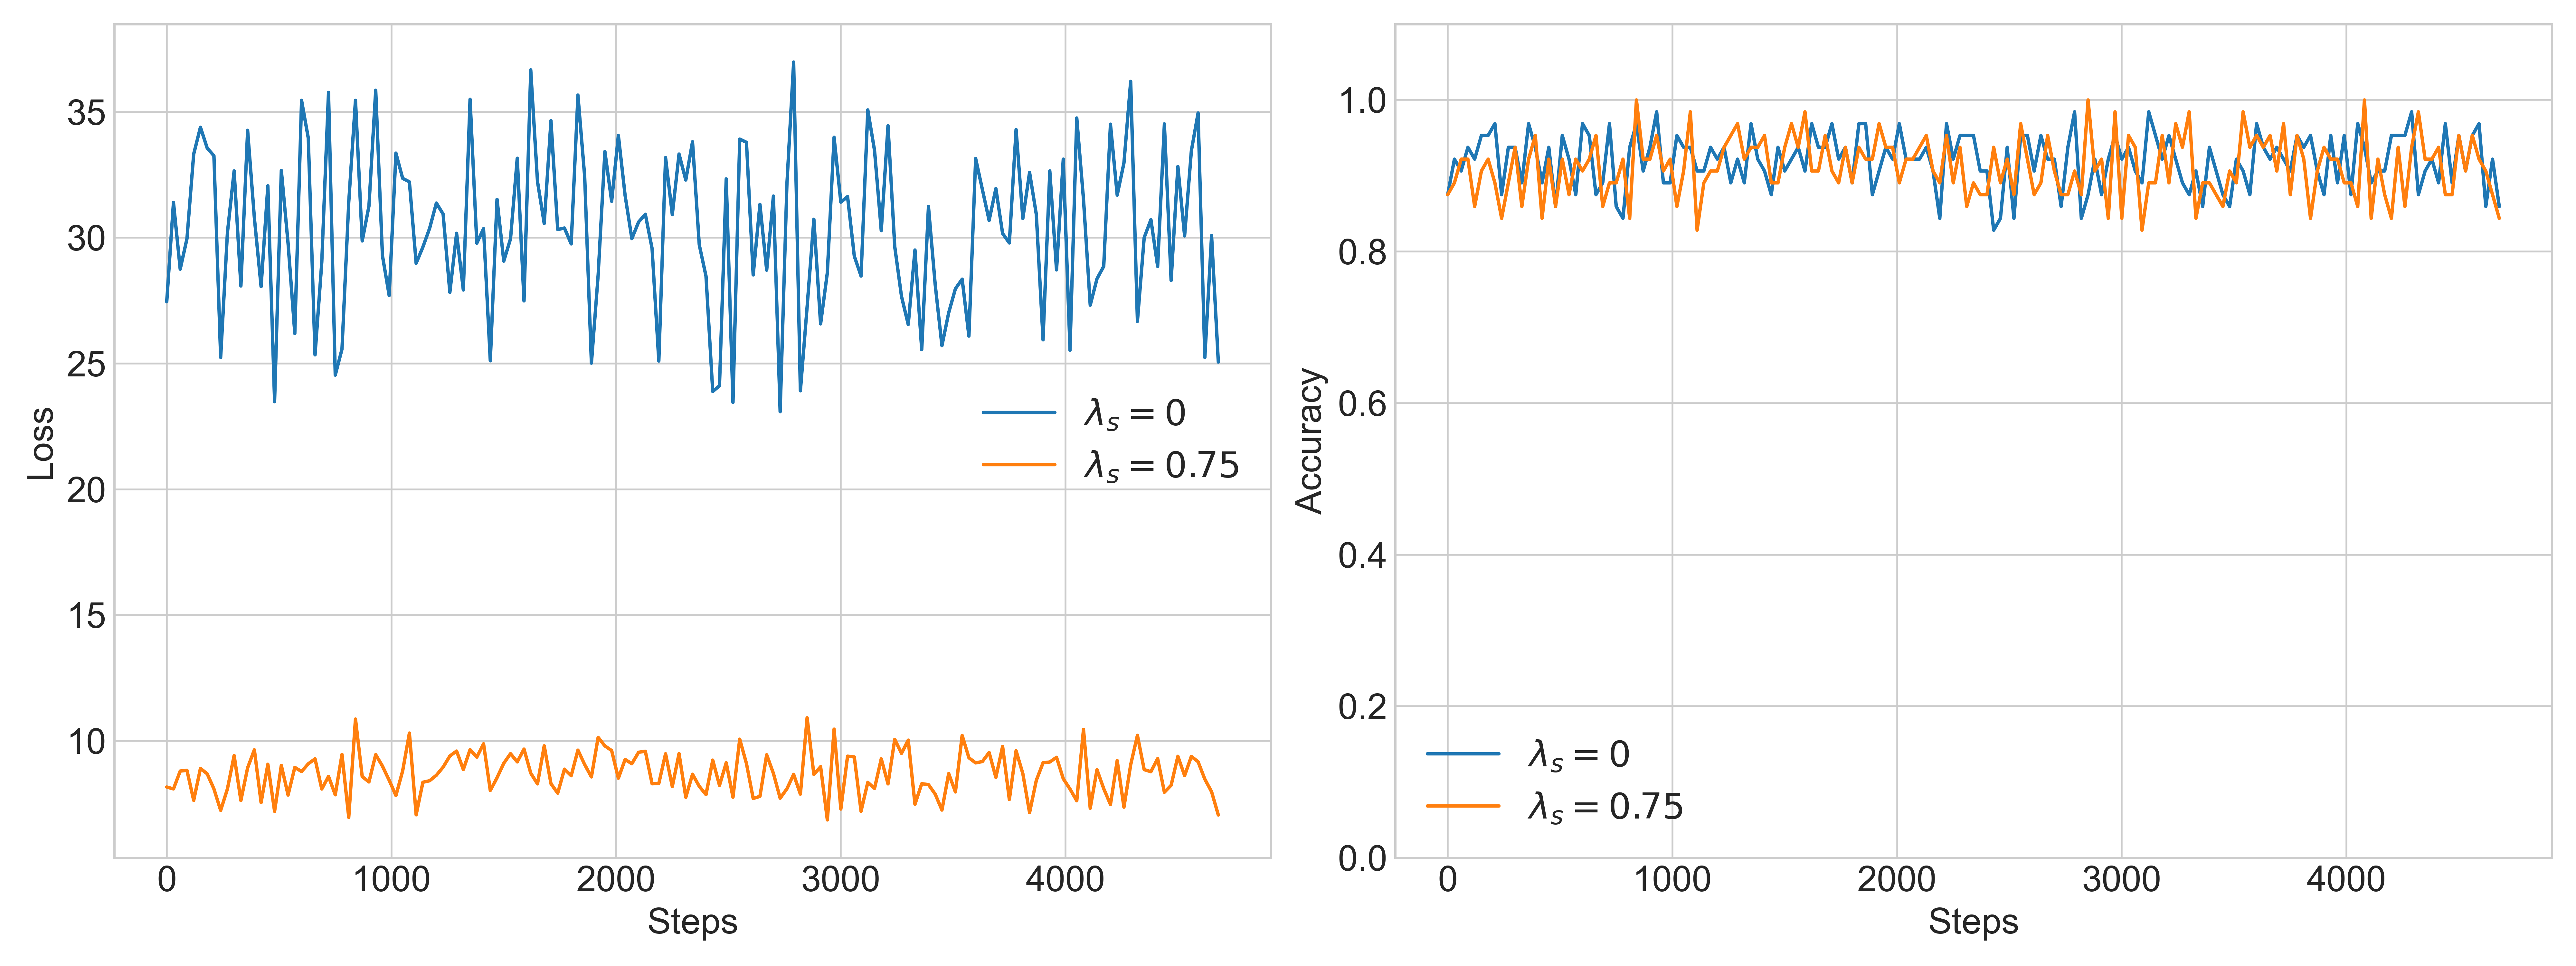
\includegraphics[width=\linewidth]{images/3dshapes_fixedListener_baseline_random_0_075_losses.png}
	\caption{Training results of reference games against a fixed listener on exhaustive captions of 3Dshapes (pure decoding, $\lambda_s=0$ vs. $\lambda_s=0.75$). Left: Total speaker training loss. Right: Listener training accuracy.}
	\label{fig:3dshapes_fixed_listener_0_075_speaker_losses_listener_acc}
\end{figure}

Similarly to MS COCO, training the speaker against a fixed listener also mitigated both structural and semantic drift (Tab.~\ref{tab:3dshapes_drift_metrics_basic_baseline}). In fact, the drift decreased even compared to the pretrained speaker. This suggests that in a smaller action space of the 3Dshapes experiment, the functional training signal from the listener pretrained on ground truth captions might be strong enough to further fine-tune the speaker towards more ground truth-like messages. However, the signal appeared to not be strong enough in order to lead to definitive increases in the overlap metrics, compared to the pretrained speaker (Tab. \ref{tab:3dshapes_drift_metrics_basic_baseline}). 

The speaker trained with the fixed listener was also evaluated with image captioning metrics. Table \ref{tab:eval_metrics_refgame} indicates that caption quality improved beyond the pretrained speaker and the joint listener baseline on almost all metrics. Therefore, these metrics additionally confirmed the mitigation of language drift and corresponding caption quality deterioration provided by the fixed listener.

\begin{figure}[h]
	\centering
	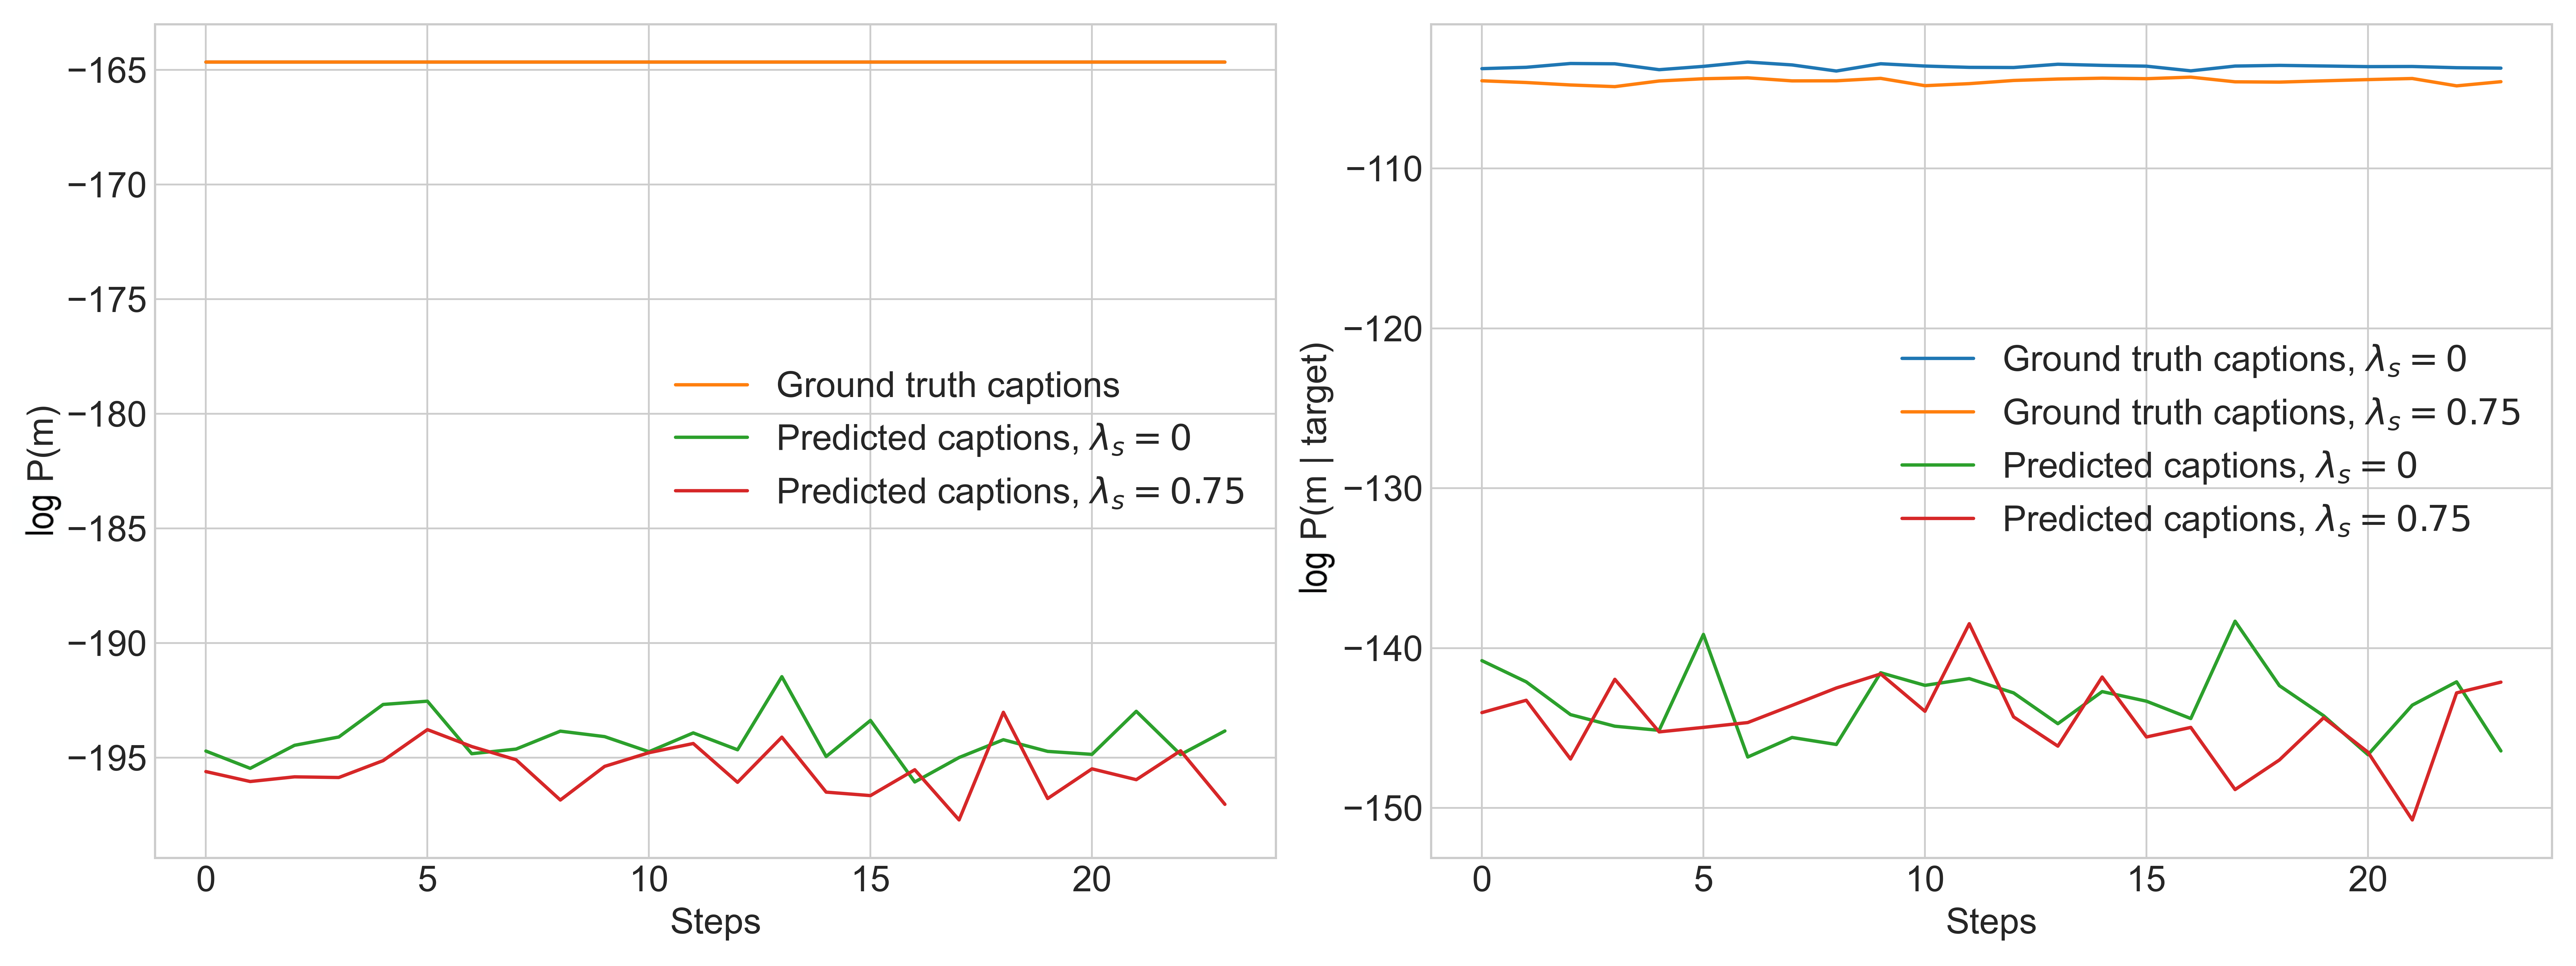
\includegraphics[width=\linewidth]{images/3dshapes_fixedListener_structural_semantic_drift_49_pure_0_075_random.png}
	\caption{Drift dynamics computed during reference game training with the fixed listener on 3Dshapes (pure decoding, $\lambda_s=0$ vs. $\lambda_s=0.75$). Higher values indicate less drift. Left: Structural drift of ground truth and predicted captions under the pretrained LM. Right: Semantic drift of ground truth and predicted captions under the pretrained speaker model.}
	\label{fig:3dshapes_fixed_listener_0_075_str_sem_drift}
\end{figure}

In order to investigate whether it was indeed the functional task signal that was responsible for mitigating the language drift, and whether better task improvement can be achieved given a stronger functional signal, a follow-up experiment with a functional loss only (i.e., $\lambda_s=0$) was also conducted for 3Dshapes. While the task success was not visibly improved (see Fig.~\ref{fig:3dshapes_fixed_listener_0_075_speaker_losses_listener_acc}, right, orange vs. blue line), structural and semantic drifts during training were indeed slightly lower for $\lambda_s=0$, compared to $\lambda_s=0.75$ (Fig.~\ref{fig:3dshapes_fixed_listener_0_075_str_sem_drift}, green line being slightly above the red one).\footnote{Semantic drift values of the ground truth are slightly different due to the known non-deterministic behaviour of some CUDA supporting RNN implementations in Pytorch, even with a random seed.} Validation results in Table \ref{tab:3dshapes_drift_metrics_basic_baseline} indicate that semantic drift was better mitigated under a stronger functional training signal ($\lambda_s =0$ compared to $\lambda_s =0.75$), suggesting that the grounding was better preserved. Structural drift, however, increased, compared to $\lambda_s =0.75$, which is expected given that there was no structural learning signal anymore in the $\lambda_s =0$ experiment. Further confirming intuitions regarding the role of the functional learning signal, the discrete overlap increased in the $\lambda_s =0$ configuration, outperforming the baseline joint listener experiment. The continuous overlap, on the other hand, decreased, compared to both pretrained and baseline joint speakers, indicating that the functional improvements might not be translated to topographic effects in the embedding space \parencite[cf.][]{lazaridou2018emergence}. Overall, results with both $\lambda_s$ configurations supported \textbf{H6}.

Additionally, in order to address the apparent overfitting and co-adaptation of the joint speaker and listener in the previous similar pairs experiment (Section~\ref{expt:3dsapes_similar}), as was apparent from the discrepancy between the training and testing accuracies (Fig.~\ref{fig:3dshapes_wShort_similarFixed_075_speaker_losses_listener_acc}, blue lines, and Tab.~\ref{tab:3dshapes_drift_metrics_basic_similar}), a follow-up experiment with a fixed listener was conducted. It also used similar pairs matching on the three fixed categories, and exhaustive captions. 
The training dynamics in Figure~\ref{fig:3dshapes_similarFixed_fixedListener_075_speaker_loss_listener_acc} were similar to the training on random pairs (cf.~Fig.~\ref{fig:3dshapes_fixed_listener_0_075_speaker_losses_listener_acc}), and resulted in a lower training accuracy than with the joint listener. The test accuracies both on the same features and different features test sets were closer to the training accuracy (Tab.~\ref{tab:3dshapes_drift_metrics_basic_similar}, last two lines), showing that the discrepancy between trainining and test accuracy in Section \ref{expt:3dsapes_similar} was at least to some extend due to speaker-listener co-adaptation on the training dataset. At the same time, the listener's accuracy did not improve beyond pretraining level (it was, in fact, worse than the pretraining test accuracy on random pairs), indicating that the speaker did not adapt her messages to functional needs much. Surprisingly, the test accuracy was higher on the different features test set than on the same features set. This could be attributed to potential differences in the listener's ability to discriminate the particular features belonging to either set, as induced by the pretraining. Compared to the accuracy difference between the test sets in the joint listener experiment, it can also be inferred that reference game fine-tuning for two epochs was not sufficient for overriding the agents' capabilities learned during pretraining in the fixed listener experiment, like communicating about features which were not part of the reference game training but were used in the pretraining.

Visually, the drift dynamics during training also did not differ between the fixed and the joint listener experiments (Fig.~\ref{fig:3dshapes_similarFixed_fixedListener_075_tr_sem_drift}~vs.~Fig.~\ref{fig:3dshapes_wShort_similarFixed_075_str_sem_drift}, blue and green lines). Interestingly, in contrast to random pairs, the semantic drift values did not improve with the fixed listener compared to the joint listener on the same features test set, but did improve on the different features test set (Tab.~\ref{tab:3dshapes_drift_metrics_basic_baseline}~vs.~Tab.~\ref{tab:3dshapes_drift_metrics_basic_similar}). The results were the other way around for structural drift. The discrete overlap was higher for both tests for the fixed listener than the joint one, and so was the continuous overlap on the different features test set.
Taken together, these results indicate that given more complex visual input, the listener grounding was more susceptible to overfitting, yet the functional signal was not strong enough so as to result in speaker-listener co-adaptation measured by semantic drift. Therefore, it seems to be a difficult task to fine-tune the speaker for a task on complex visual input in a way that provides a sufficiently strong task success signal, while also achieving a good generalization performance.

\begin{figure}[h]
	\centering
	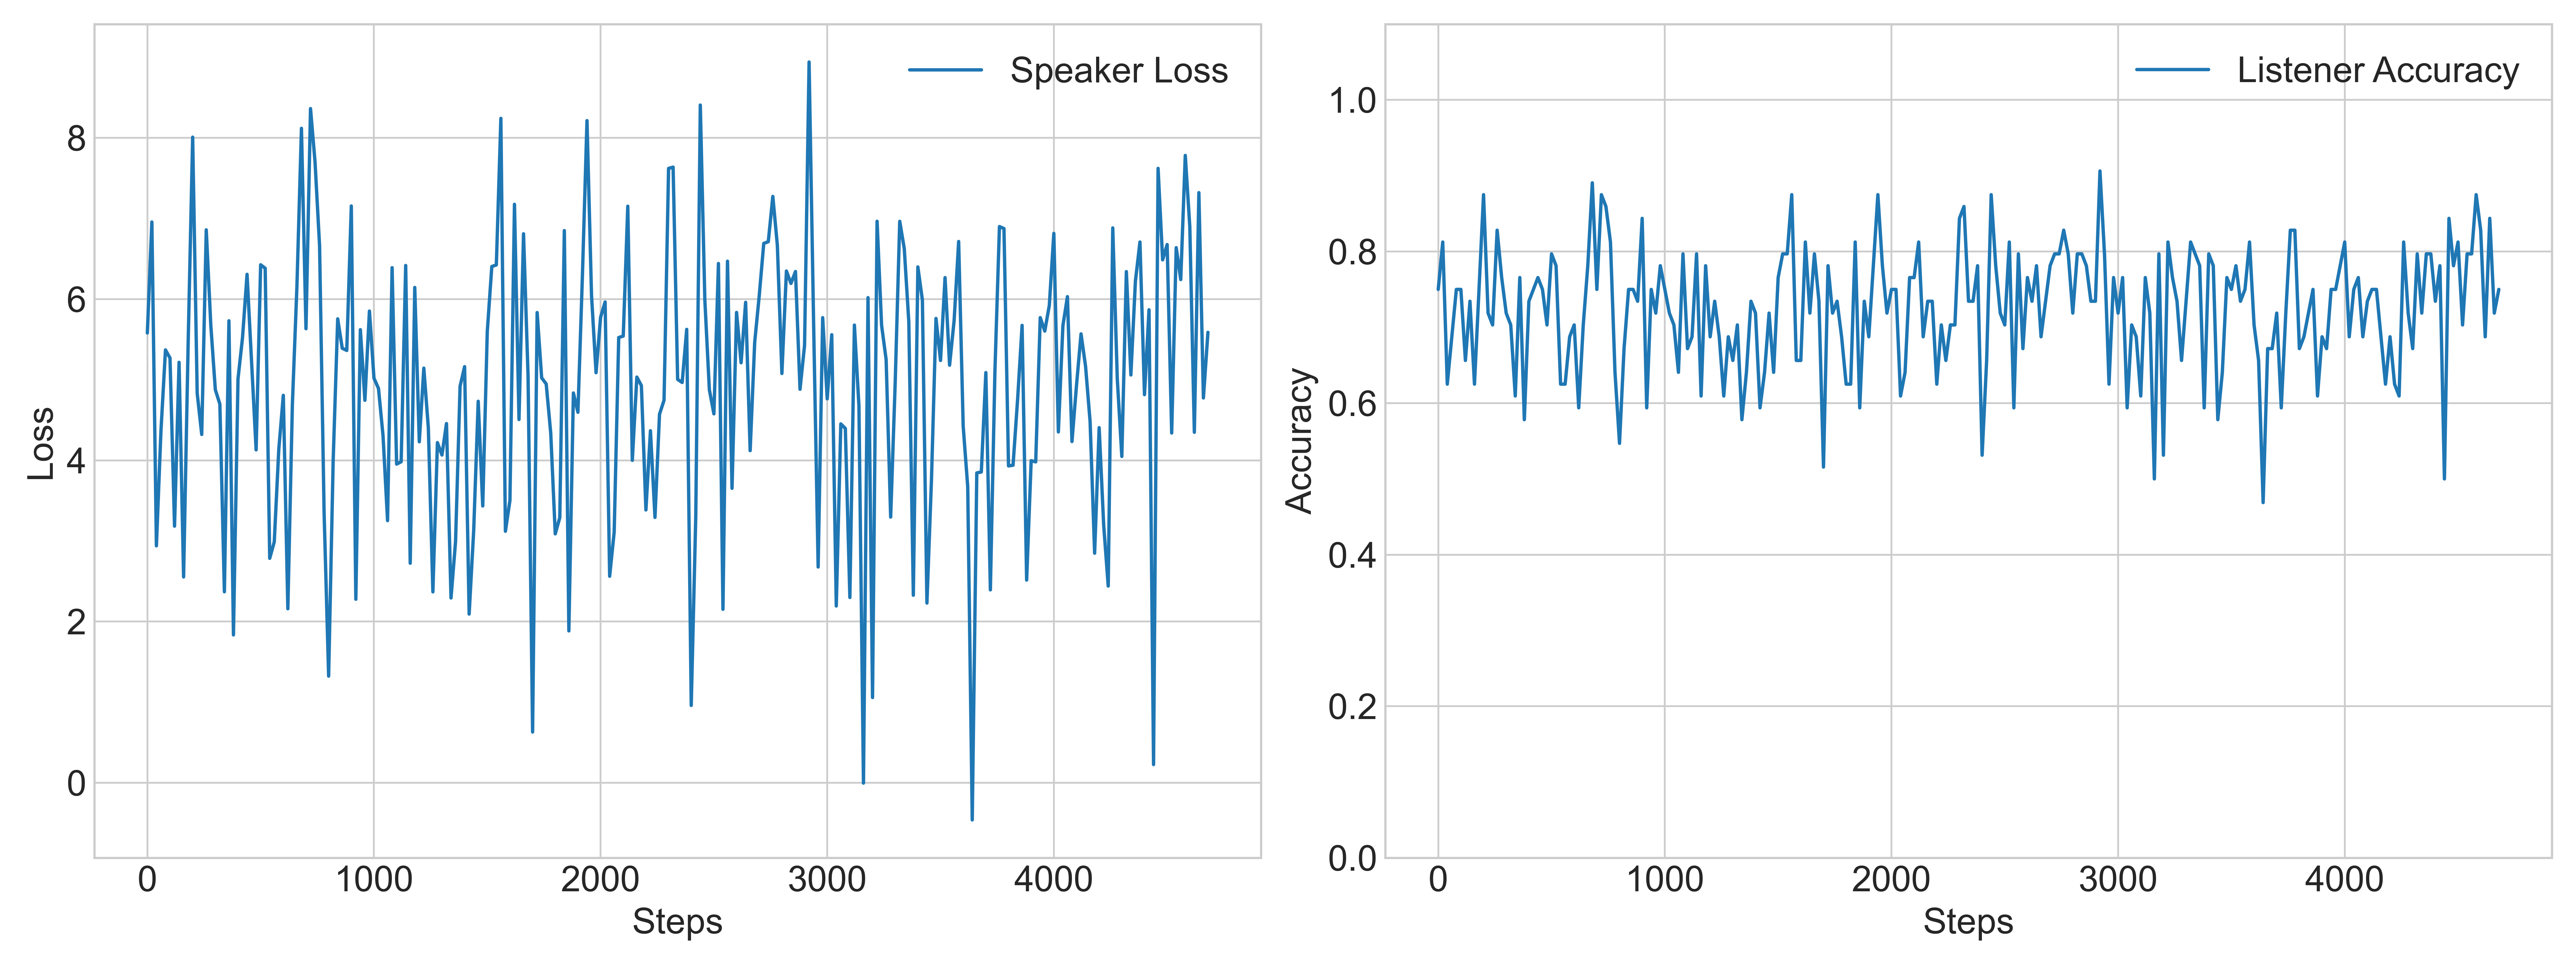
\includegraphics[width=\linewidth]{images/3dshapes_fixedListener_similarFixed_exh_075_losses.png}
	\caption{Training results of the 3Dshapes experiment on similar image pairs with fixed matching features with a fixed listener (pure decoding, exhaustive captions, $L_s = 0.75$). Left: Total speaker training loss. Right: Listener training accuracy.}
	\label{fig:3dshapes_similarFixed_fixedListener_075_speaker_loss_listener_acc}
\end{figure}

\begin{figure}[h]
	\centering
	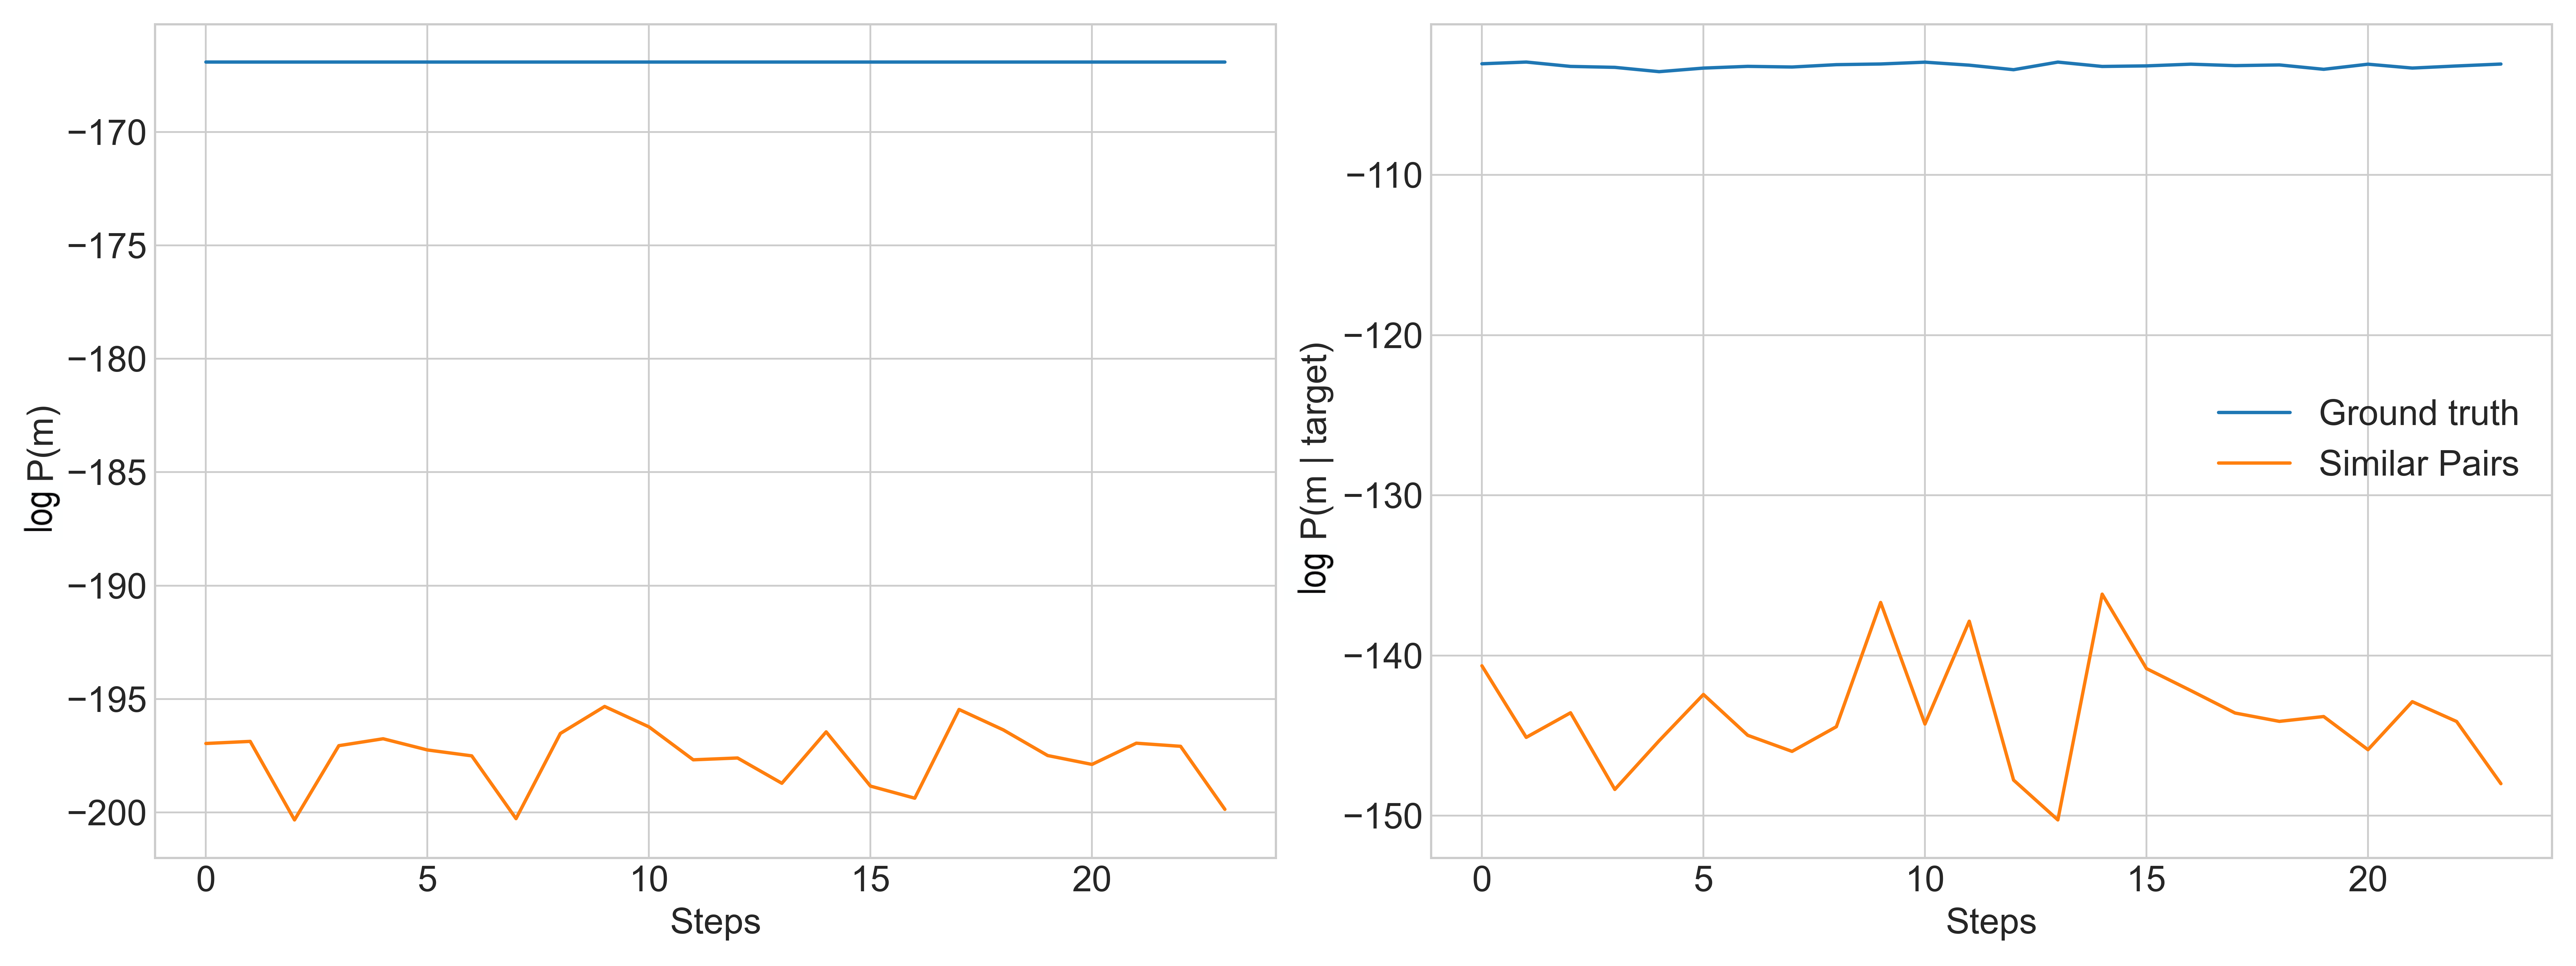
\includegraphics[width=\linewidth]{images/3dshapes_structural_semantic_drift_fixedListener_similarFixed_075.png}
	\caption{Drift dynamics computed during training of the 3Dshapes experiment on similar image pairs with fixed matching features with a fixed listener (pure decoding, exhaustive captions, $L_s = 0.75$). Left: Structural drift of ground truth and predicted captions under the pretrained LM. Right: Semantic drift of ground truth and predicted captions under the pretrained speaker model.}
	\label{fig:3dshapes_similarFixed_fixedListener_075_tr_sem_drift}
\end{figure}

To sum up, \textbf{H6} is also supported by the results of the 3Dshapes experiment with random image  pairs. Similarly to MS COCO, one can infer that reference game performance was at least partly carried by speaker-listener co-adaptation with the joint listener, and that the training signal available from the pretrained listener might both have structural effects in this smaller action space and mitigate semantic drift. 
Additionally, it was shown that training with a fixed listener on more complex visual input like similar image pairs did not provide conclusive support for \textbf{H6}, but instead revealed difficulties in grounding the joint listener in such complex input. Taken together, a complex interaction between the agents' co-adaptation, their task success capacity and the complexity of their input became apparent in these experiments.

\subsection{3Dshapes: Short Captions Experiments}
\label{expt:3dshapes_short}

\begin{table}[] 
	\begin{tabularx}{\textwidth}{|X|l|l|X|X|X|}
		\hline
		\textbf{Model name}                                    & \textbf{log $P(m)$} & \textbf{log $P(m \mid i)$} & \textbf{Overlap (d)} & \textbf{Overlap (c)} & \textbf{Acc.} \\ \hline
		Ground truth mixed       &     -139.026            &    -80.323             &       7.401        &        0.028        &                         \\ \hline
		Pretrained 3D mixed speaker    &      -192.903           &         -59.623               &        2.309              &      -0.001                & 0.944 (3D Short random listeners)        \\ \hline
		%3D Baseline, random  &       -195.495        &           -147.313           &          5.247            &         0.001             & 0.979                                    &                        0.959                   \\ \hline
		%3D Baseline, similar all, $\lambda_s = 0.75$ &      -198.189             &       -140.786                 &           5.578           &        0.001              & 0.878                      &            0.906                        \\ \hline
		%3D Baseline, similar fixed, random test &       -193.709            &    -141.010                  &        3.280            &      -0.003         &            0.688       &                           \\ \hline
		%3D Baseline, similar fixed, same test &      -199.014        &        -146.280           &        2.875       &      0.029   &              &          0.691                   \\ \hline
		%3D Baseline, similar fixed, diff. test &     -194.510     &    -146.557          &   2.071      & 0.020    &                &              0.570          \\ \hline
		3D Short, random&      -189.285             &      -58.278                  &             2.316        &         0.000             &                   0.957      \\ \hline
		3D Short, similar all, $\lambda_s = 0.75$&     -194.183        &   -59.371           &    1.032       &   0.000        &        0.791       \\ \hline
		%3D Short, similar fixed, random test&      -188.249           &     -121.830                  &             1.839         &         -0.001             &                   0.726         \\ \hline
		3D Short, similar fixed, same test&      -192.130      &     -58.753      &   0.837      & 0.003   &     0.723                \\ \hline
		3D Short, similar fixed, diff. test &  -187.713       & -57.257     & 1.915        &  0.002   &    0.564       \\ \hline
	\end{tabularx}
	\caption{\label{tab:3dshapes_drift_metrics_basic_short} Language drift metrics and listener test accuracies (``Acc.'') of experiments on the 3Dshapes dataset including short annotations. 
		``Baseline'' refers to the setup wherein the listener is trained jointly with the speaker, using pure decoding, using exhaustive captions only. ``Random'' refers to speakers trained on random target-distractor pairs; ``similar'' refers to speakers trained on similar target-distractor pairs. $\lambda_s = 0.75$ is used in all experiments. ``Mixed'' and ``short'' refers to experiments and tests with annotation of varying lengths.}
\end{table}

The goal of these experiments was to address \textbf{H8} by conducting experiments wherein the speaker produced captions of varying granularity.
To this end, the second speaker pretrained on mixed-length captions (i.e., both exhaustive and short captions) was used (see Section \ref{speaker_pretraining}). During reference game training, the structural loss was also computed against ground truth captions of varying lengths. That is, the targets that the speaker had to refer to during training were associated with either exhaustive or short ground truth captions. Otherwise, the training followed the general procedure.

These experiments addressed several aspects. First, they addressed the question whether the presence of exhaustive captions (as was the case in the baseline experiment) was necessary for successful task completion. Second, they addressed whether absence of exhaustivity might be the reason for language drift because the speaker might have to resort to drift strategies in order to complete the functional task due to a lack of linguistic task-appropriate resources. 
Third, speaker flexibility to generate messages of variable length in absence of explicit message length regularization was investigated. 

\begin{figure}[h]
	\centering
	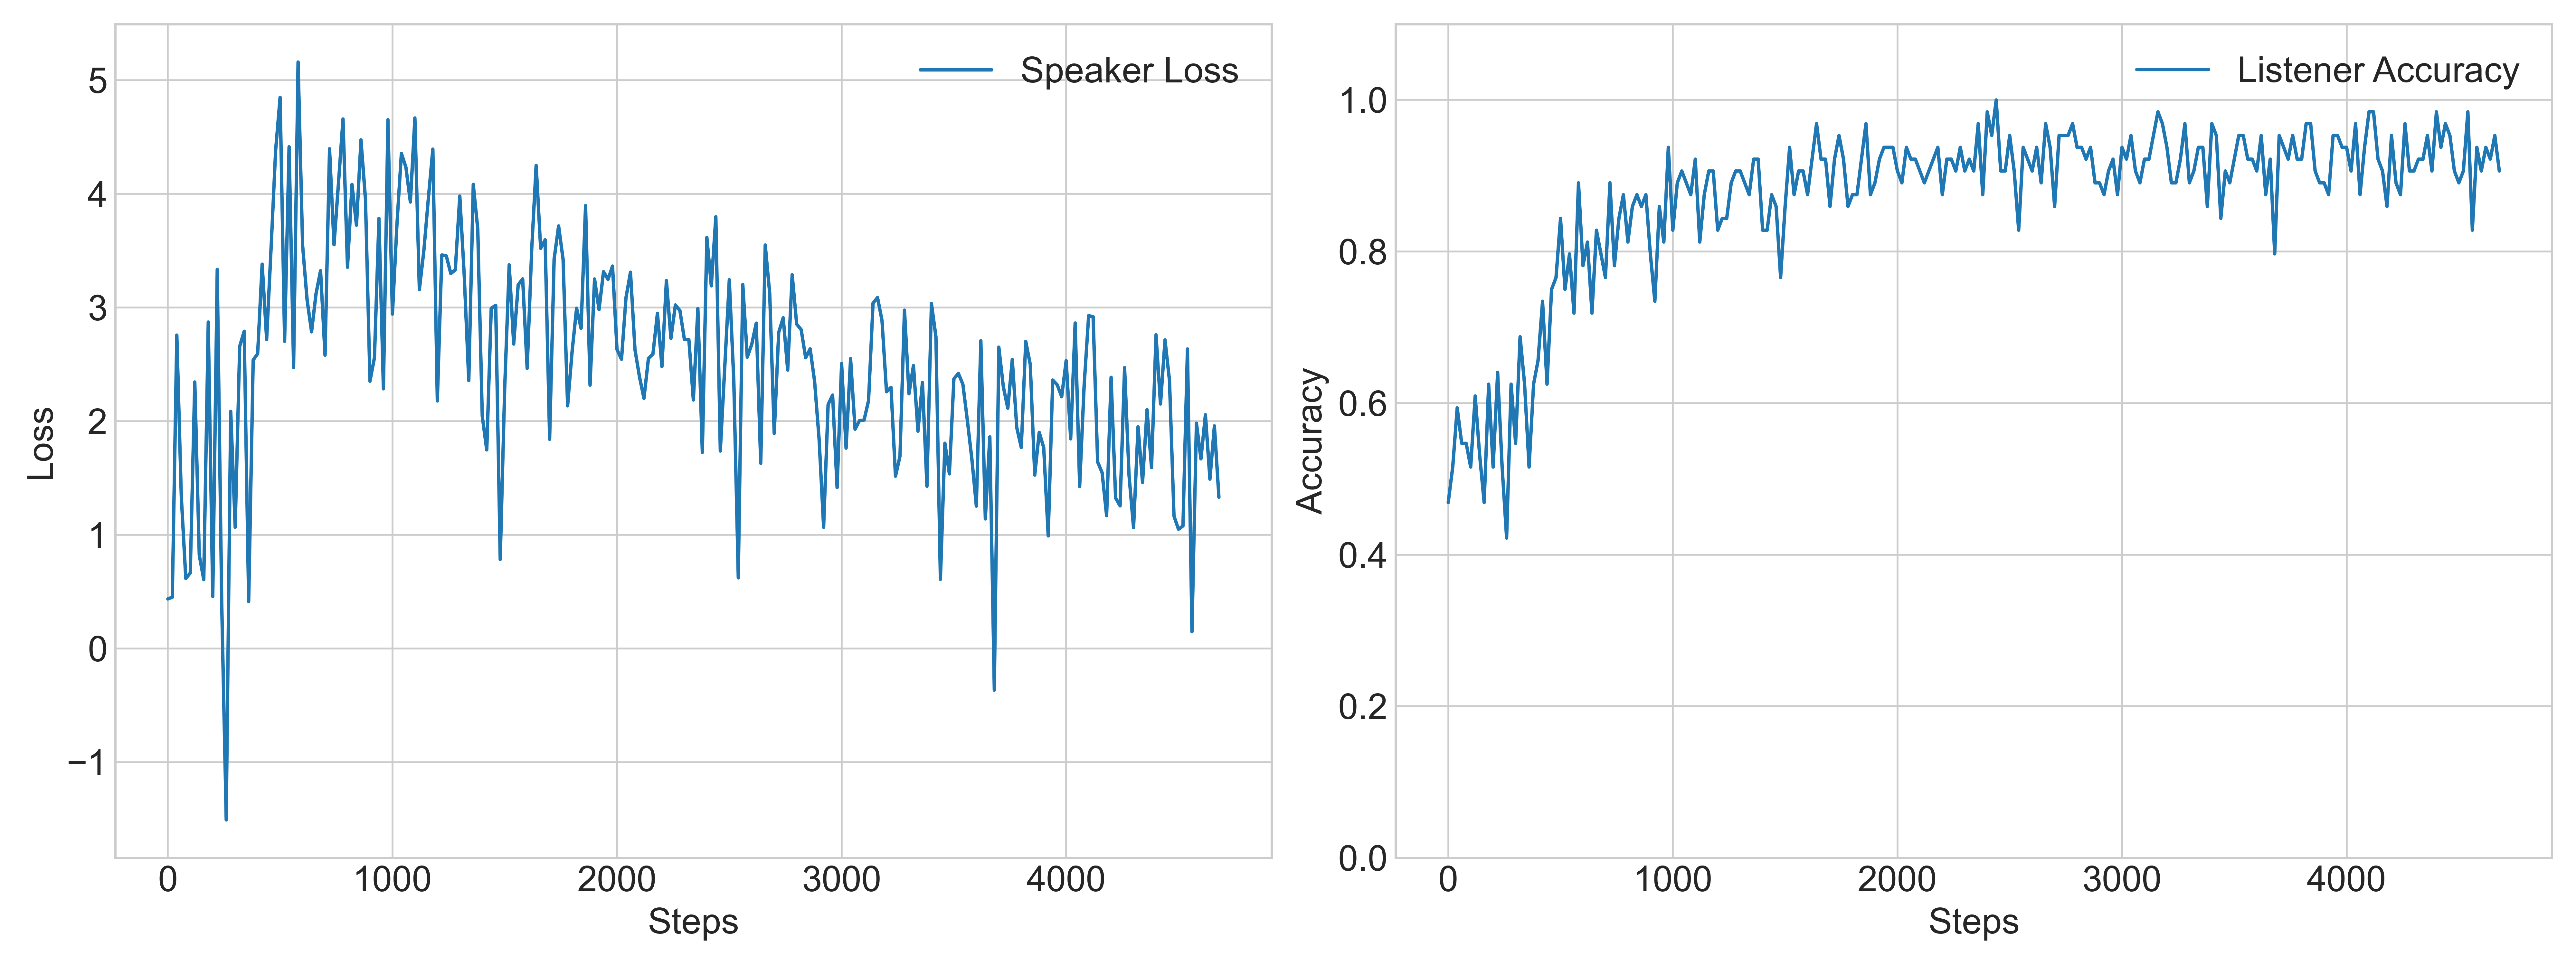
\includegraphics[width=\linewidth]{images/3dshapes_wShort_baseline_random_075_losses.png}
	\caption{Training results of the baseline reference game on both short and exhaustive captions of 3Dshapes (pure decoding, $\lambda_s=0.75$). Left: Total speaker training loss. Right: Listener training accuracy.}
	\label{fig:3dshapes_wShort_075_speaker_losses_listener_acc}
\end{figure}

First, the baseline experiment with pure decoding and $\lambda_s = 0.75$ was conducted with the mixed captions. Similar to the testing procedure in previous experiments, the model was evaluated in terms of listener accuracy and language drift on the same 1,000 held out images. For the test set, it was now also chosen at random whether a target image was associated with three short or exhaustive ground truth captions out of five, in order to compute drift metrics of the ground truth captions. Therefore, the drift measures of the ground truth differ from the exhaustive ground truth captions.
The training results can be seen in Figure~\ref{fig:3dshapes_wShort_075_speaker_losses_listener_acc}. Based on visual comparison to the exhaustive captions baseline experiment (Fig.~\ref{fig:3dshapes_baseline_speaker_loss_listener_acc_all}, red lines), no qualitative differences in either speaker convergence or listener training performance could be observed. Nonetheless, listener test accuracy decreased by 0.022 compared to exhaustive baseline (Tab.~\ref{tab:3dshapes_drift_metrics_basic_short}).
This rather small difference could be because in this experiment the target and distractor images were paired at random and were, therefore, likely quite dissimilar, intuitively rendering the presence of exhaustive messages not necessary for successful reference. Example short messages generated by this speaker are showed in Figure~\ref{fig:shapes_randPairs_speaker_generations}.

Turning towards language drift, one can observe that both structural and semantic drift during training were lower for this experiment compared to the exhaustive experiment (Fig.~\ref{fig:3dshapes_wShort_075_str_sem_drift} vs. Fig.~\ref{fig:3dshapes_baseline_all_str_sem_drift}, red lines), showing the opposite to the hypothesized effect. The lower structural drift could be attributed to generally higher naturalness of the short captions compared to the exhaustive ones, thus, rendering them more likely under a pretrained LM. The lower semantic drift which additionally was lower for the generated captions than for the ground truth ones might indicate that the speaker was further fine-tuned to produce messages that were more likely under the pretrained speaker generation strategy. This might be easier than for exhaustive captions because of the shorter effective message length which is advantageous for RNN training \parencite[cf.][]{jaeger2002tutorial}. This is further cofirmed by the test drift results. Structural drift was lower compared to both the exhaustive baseline and the pretrained speaker. However, the absolute difference to the drift value of the ground truth captions was much larger for mixed captions (50.259) compared to the exhaustive captions (30.743) (Tab.~\ref{tab:3dshapes_drift_metrics_basic_short}). This might suggest that due to the varying length of messages and the respective variation in sentence structure the speaker might struggle more to produce syntactically well-formed sentences after fine-tuning. 
Similarly, semantic drift was lower for mixed captions compared to the both exhaustive and pretrained speakers. The absolute difference in semantic drift of the fine-tuned speaker and the ground truth captions was 22.045 for mixed captions and 39.457 for the exhaustive experiment, where in the former the speaker actually improved over ground truth captions, while the latter was worse (Tab.~\ref{tab:3dshapes_drift_metrics_basic_short}). This might indicate that further supervised fine-tuning of the speaker model took place for the mixed but not the exhaustive captions. Again, this could be attributed to the effective message length difference of the ground truth captions and the respective difficulty of training.
Regarding overlap metrics, the discrete overlap decreased much more drastically compared to ground truth for the mixed captions than for exhaustive ones. This low value might be confounded with the variation of the granularity of a sampled ground truth caption, and not be directly representative of functional performance. For instance, during evaluation, the speaker might have generated a valid discriminative short caption, but the sampled corresponding ground truth was an exhaustive caption, yielding a low overlap value. Overall, however, absence of exhaustive captions did not lead to `strategic' language drift.  

\begin{figure}[h]
	\centering
	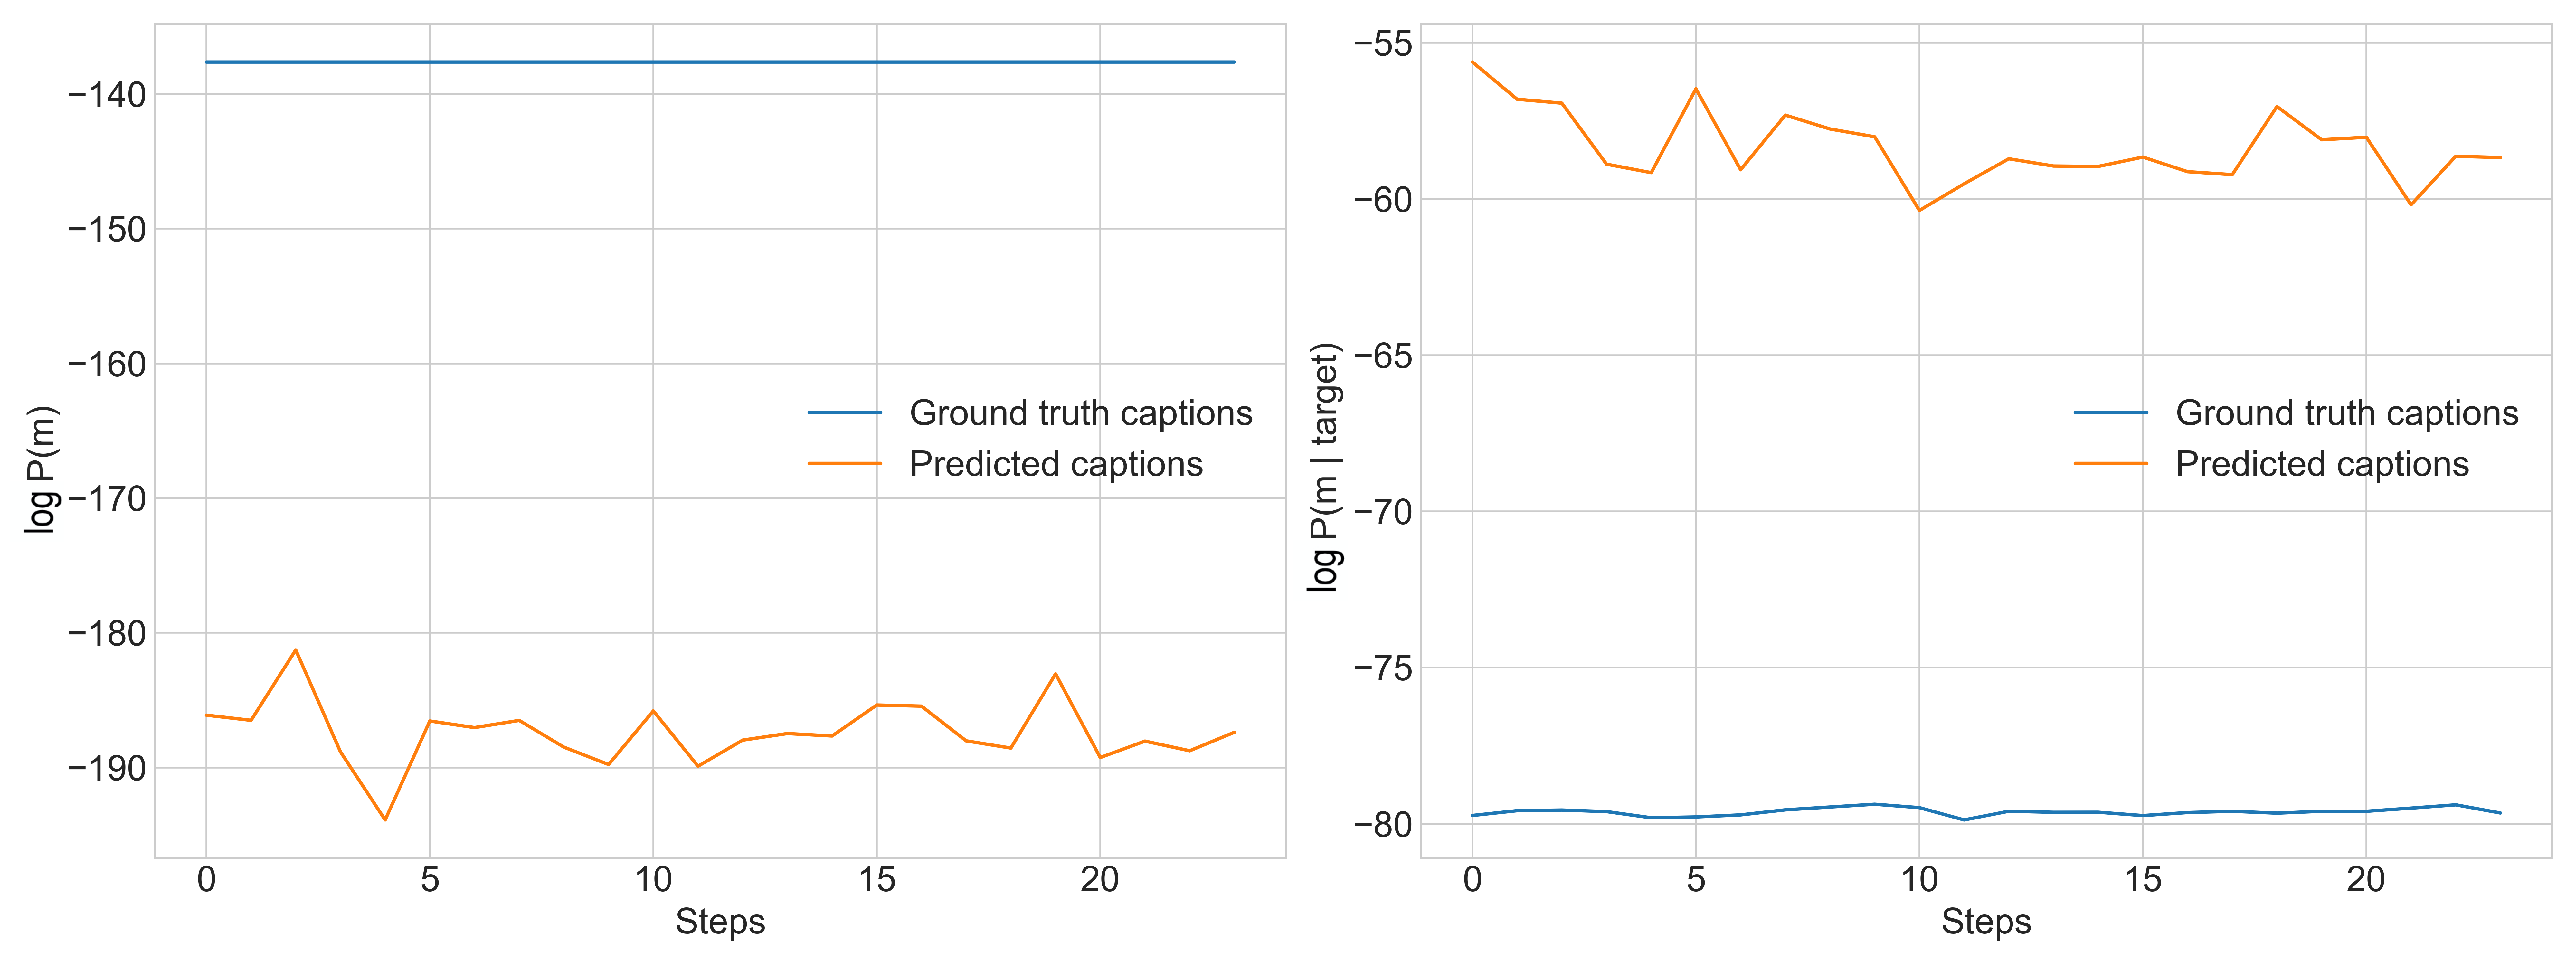
\includegraphics[width=\linewidth]{images/3dshapes_wShort_structural_semantic_drift_49_pure_075_random.png}
	\caption{Drift dynamics computed during reference game training on both short and exhaustive captions of 3Dshapes (pure decoding, $\lambda_s=0.75$). Higher values indicate less drift. Left: Structural drift of ground truth and predicted captions under the pretrained LM. Right: Semantic drift of ground truth and predicted captions under the pretrained speaker model.}
	\label{fig:3dshapes_wShort_075_str_sem_drift}
\end{figure}

In order to investigate the third aspect---speaker's generation length flexibility---lengths of the captions generated by the speaker on the validation set were computed. These were calculated by counting the number of tokens until the first occurrence of the special \texttt{END} token in the message (excluding it). As can be seen in Figure~\ref{fig:3dshapes_exh_short_random_lengths}, the speaker that saw short captions during pretraining and in the reference game has learned to produce captions with varying length with approximately uniform probability, except for a bias towards generating captions of maximal allowed length around one third of the time. This bias can also be observed for the exhaustive captions speaker, whose generated caption lengths matched the ones from the exhaustive training set. These results hint at the importance of the training data distribution for the speaker's potential to adjust her message length, possibly responding to different granularity needs (see below for details). 

\begin{figure}[h]
	\centering
	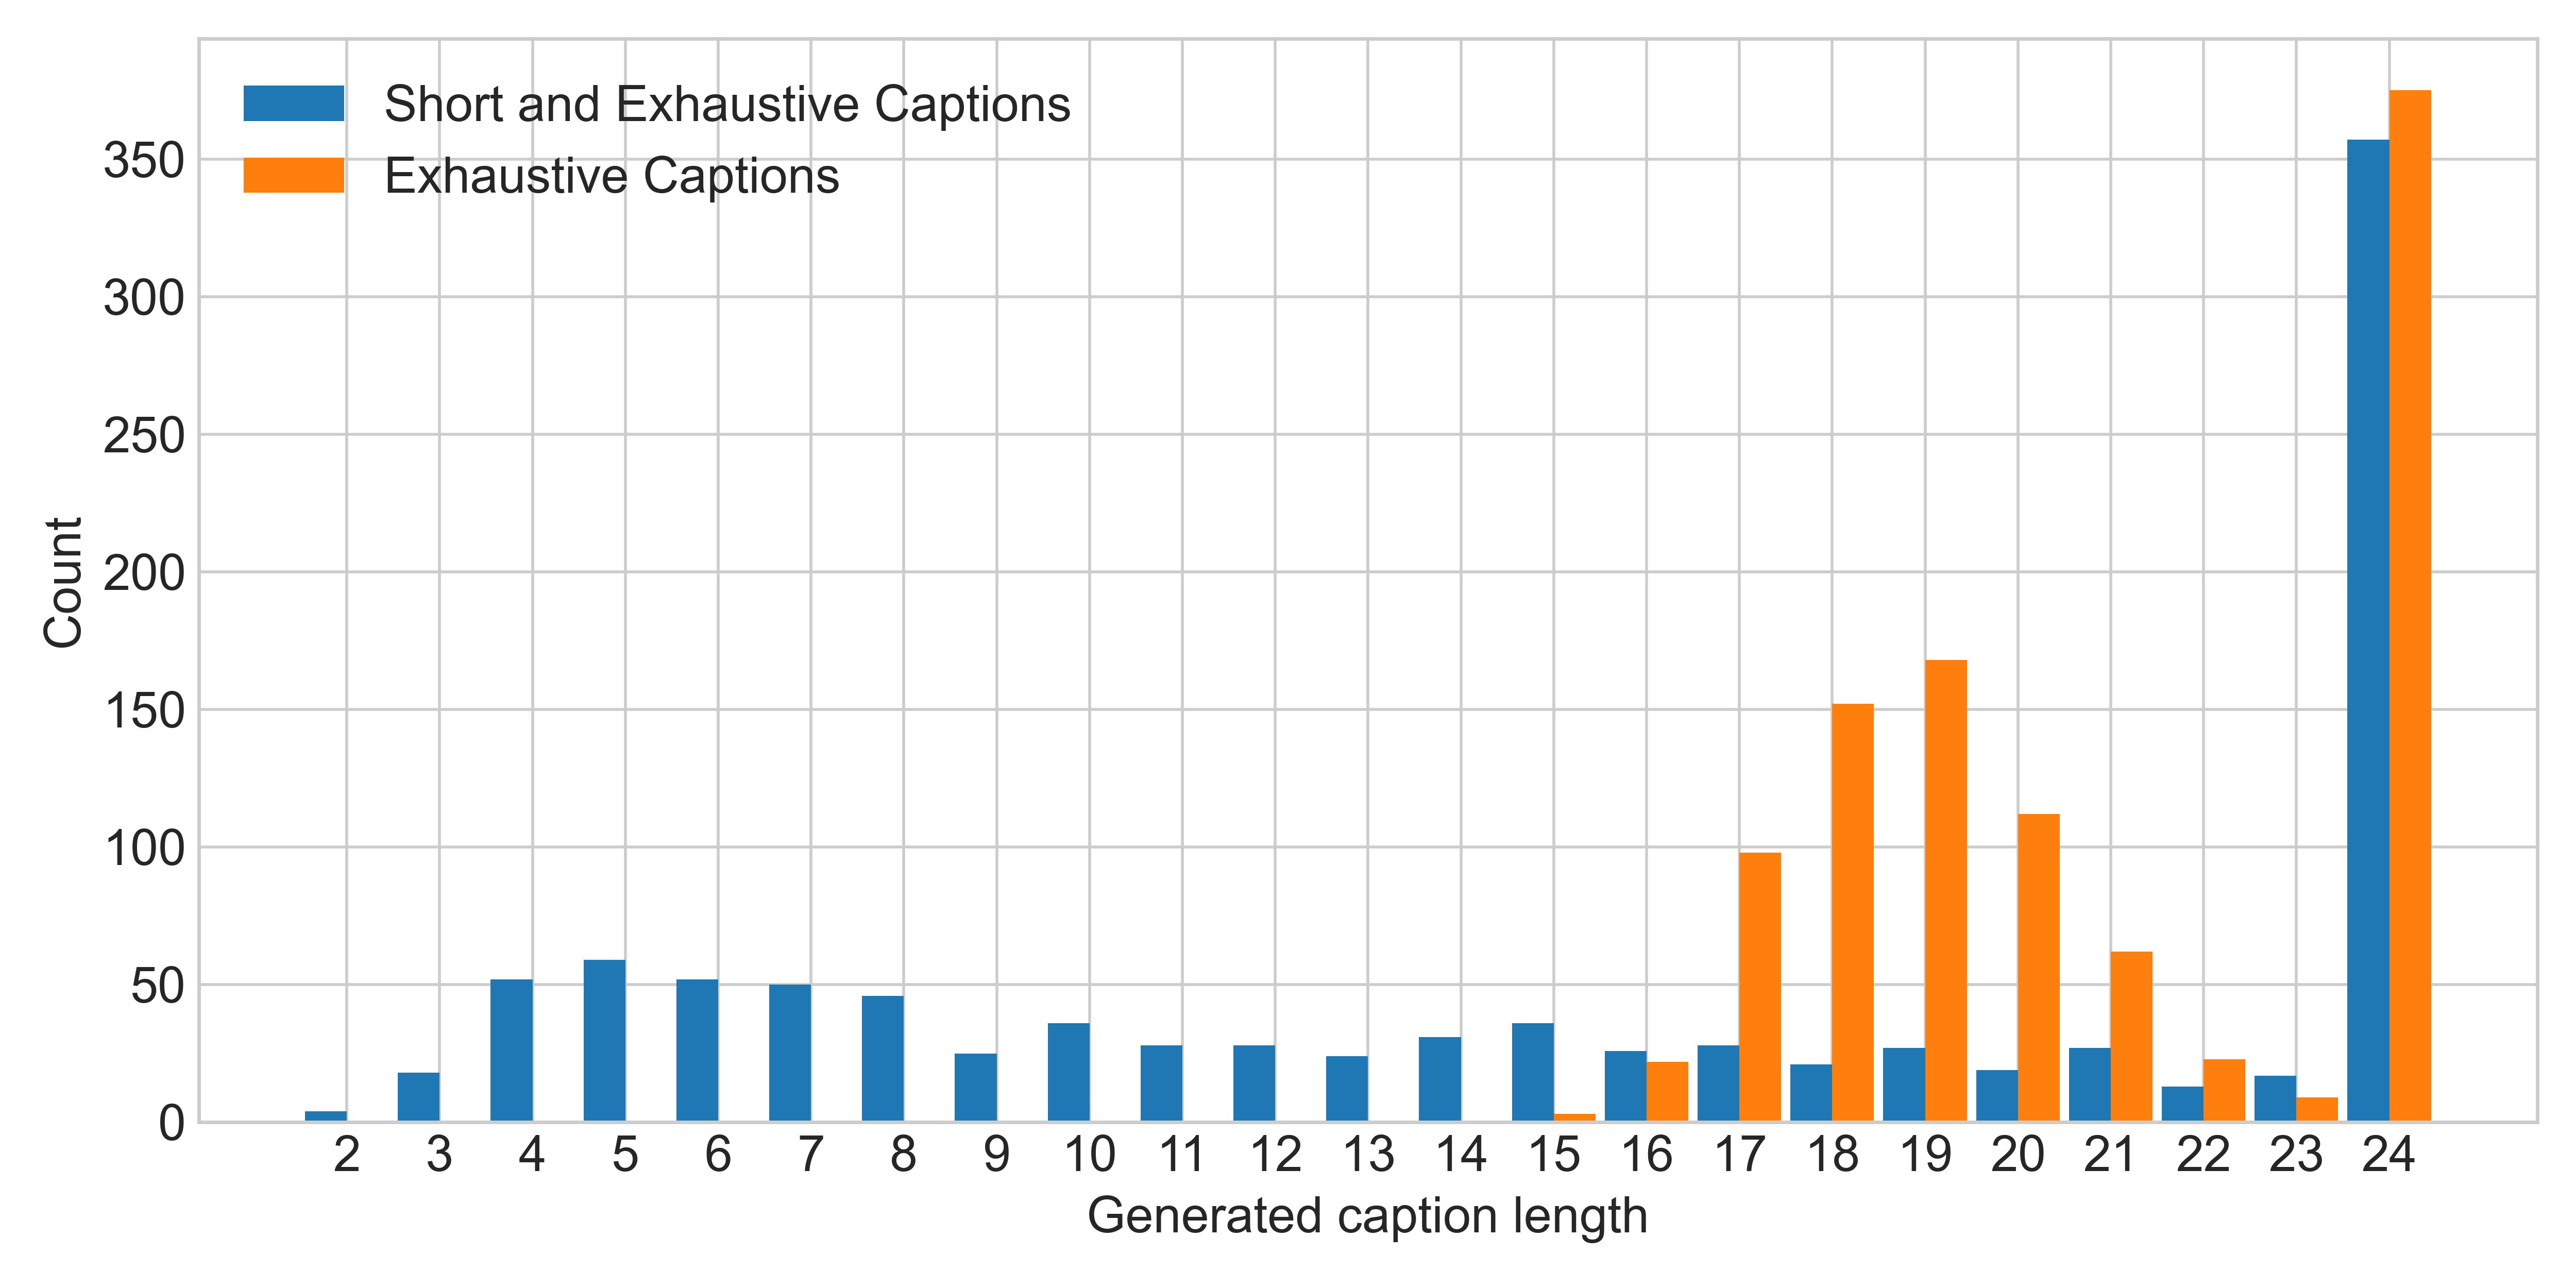
\includegraphics[width=0.7\linewidth]{images/3dshapes_exh_short_random_length_counts.png}
	\caption{Counts of effective sentence lengths generated on the validation dataset by the speakers from the exhaustive and the mixed-length experiments.}
	\label{fig:3dshapes_exh_short_random_lengths}
\end{figure}

In sum, \textbf{H8} was not supported by experimental results on random target-distractor pairs. In fact, language drift was even smaller compared to the exhaustive captions experiment. This suggests that architectural aspects like the length of messages the speaker was trained to generate have a larger influence on message quality than guaranteed presence of fully descriptive captions in the training dataset. At the same time, these results showed that the speaker was capable of flexibly varying her message length, if the respective inductive bias was provided during training. 

\subsubsection{Similar Pairs Experiment}
\label{expt:3d_similar}

In order to increase the pressure towards the necessity of exhaustive descriptions, an experiment including short captions was conducted on \emph{similar} target-distractor image pairs. Again, the similar pairs were constructed such that the target and the distractor matched with respect to object shape, object color and background color. Since this set up allows for more detailed analyses, the set up akin to the first experiment in Section \ref{expt:3dsapes_similar} (where all features were used for matching the pairs) is omitted for the mixed captions. The results of the comparable similar pairs experiment with exhaustive captions are discussed in Section \ref{expt:3dsapes_similar}. The effect of adding short captions during training compared to using exhaustive captions only can be seen in Figure~\ref{fig:3dshapes_wShort_similarFixed_075_speaker_losses_listener_acc} which shows that training the speaker on mixed length captions did not visibly influence the training dynamics compared to exhaustive captions only. However, similarly to exhaustive captions results, the listener's test performance on held out image pairs, both matching along the same and along different features, was much worse than training accuracy (0.723 and 0.564, respectively, see Tab.~\ref{tab:3dshapes_drift_metrics_basic_short}). This discrepancy was comparable to the exhaustive experiments, indicating that potential overfitting cannot be attributed to the difficulty of learning longer messages. Language drift results in Table \ref{tab:3dshapes_drift_metrics_basic_short} indicated a lower structural drift than for the exhaustive speaker compared to the respective pretrained speaker, suggesting that this drift is driven by message length as in the random pairs experiments, and is not as much influenced by perceptual context. Just as in the case of the exhaustive speaker in the similar pairs experiment, semantic drift also did not increase compared to the pretrained speaker, so no speaker-listener co-adaptation was observed. However, similarly to the random pairs experiment including mixed length captions, the semantic drift of the generated captions was tangibly lower than the drift of the ground truth captions (Tab.~\ref{tab:3dshapes_drift_metrics_basic_short}), which already became apparent during training (Fig.~\ref{fig:3dshapes_wShort_similarFixed_075_str_sem_drift}, right, red line being above the orange line). Following the random pairs experiment, this could be attributed to easier training of the speaker on shorter messages and resulting further fine-tuning of the speaker during the reference game, even on complex visual input. 

In this experiment, a larger discrete overlap can be observed for the different features test set than for the same features test set, and no increase in continuous overlap compared to baseline can be seen. This might suggest that the speaker can more easily fall back to the messages applicable to different features which were learned during pretraining when the messages are shorter. So the first two aspects of the short captions experiments were not influenced much by the similar pairs input, compared to the random pairs results.%On the other hand, this might indicate that the speaker was more successful in learning to refer to novel features not present in the ground truth captions with shorter messages, compared to the random pairs experiment with short captions. 
\begin{figure}[h]
	\centering
	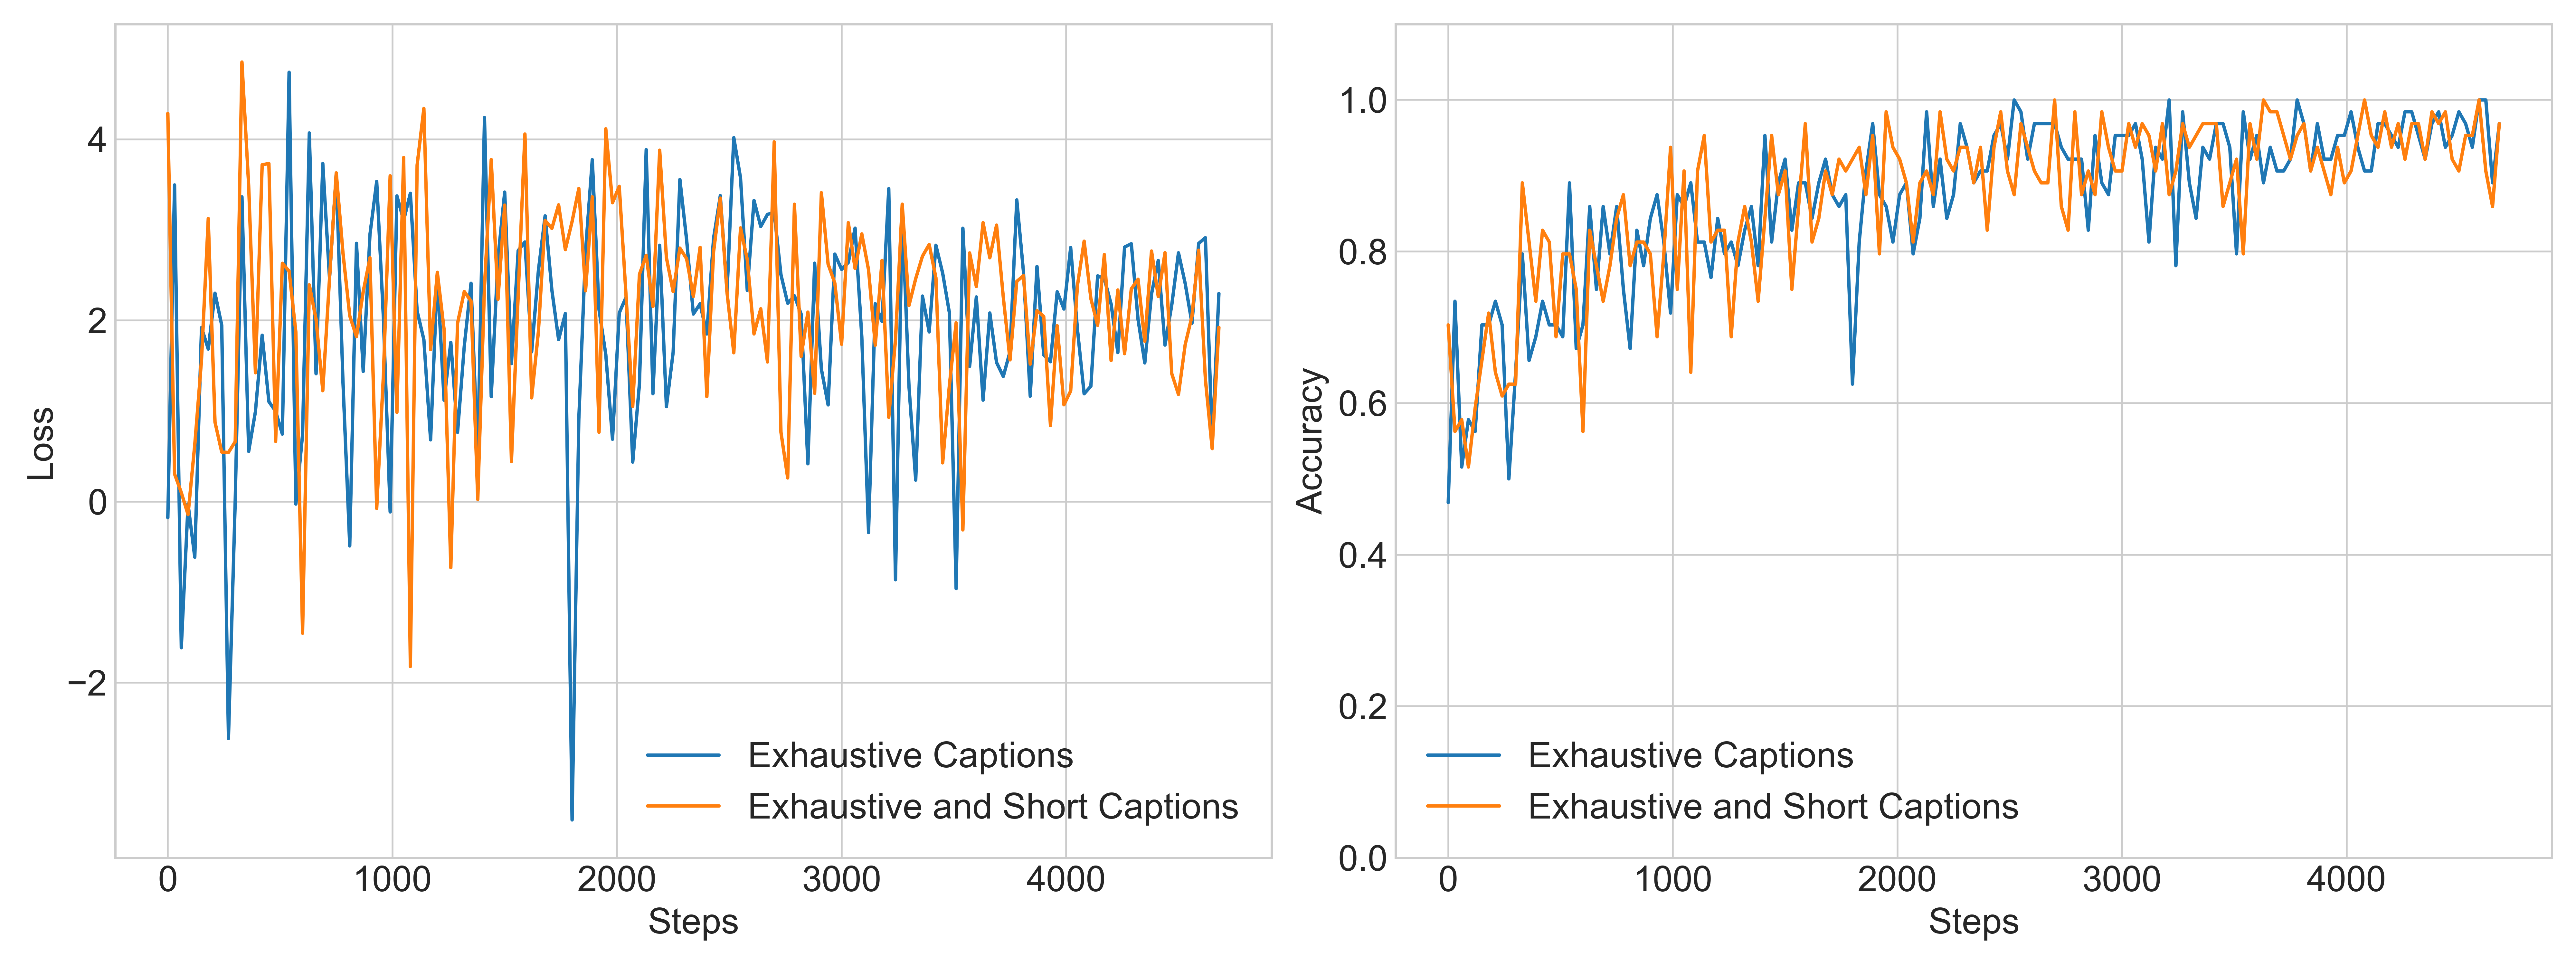
\includegraphics[width=\linewidth]{images/3dshapes_similarFixed_short_vs_exh_075_losses.png}
	\caption{Training results of the baseline reference game on both short and exhaustive captions of 3Dshapes on similar image pairs. Similar features were fixed (pure decoding, $\lambda_s=0.75$). Left: Total speaker training loss. Right: Listener training accuracy.}
	\label{fig:3dshapes_wShort_similarFixed_075_speaker_losses_listener_acc}
\end{figure}

\begin{figure}[h]
	\centering
	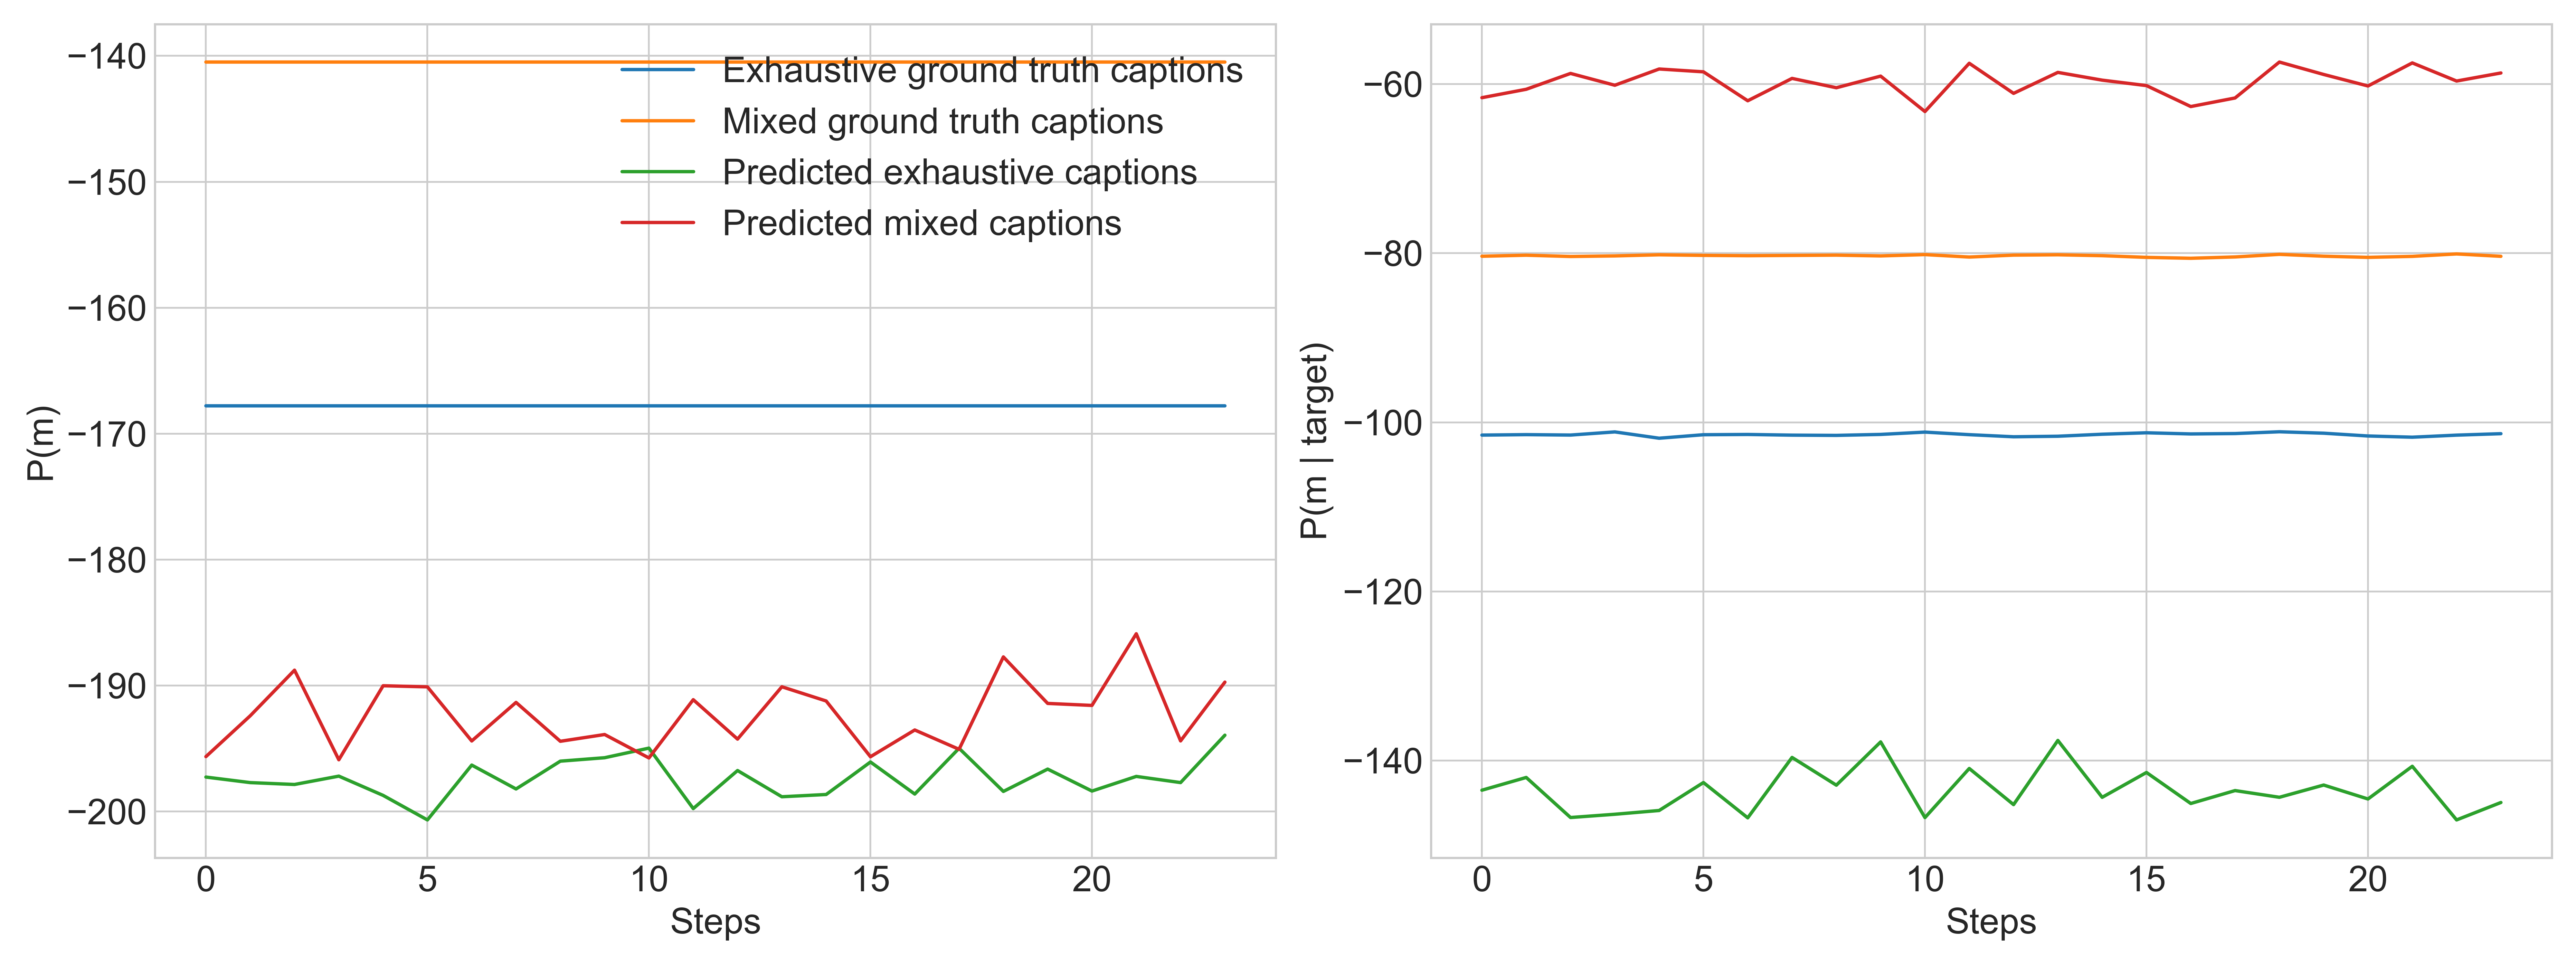
\includegraphics[width=\linewidth]{images/3dshapes_exh_short_structural_semantic_drift_49_pure_075_similarFixed.png}
	\caption{Drift dynamics computed during reference game training on similar fixed pairs on both short and exhaustive captions of 3Dshapes (pure decoding, $\lambda_s=0.75$). Higher values indicate less drift. Left: Structural drift of ground truth and predicted captions under the pretrained LM. Right: Semantic drift of ground truth and predicted captions under the pretrained speaker model.}
	\label{fig:3dshapes_wShort_similarFixed_075_str_sem_drift}
\end{figure}

Addressing the main question whether the speaker could flexibly adjust the granularity of her messages based on the difficulty of referring to discriminative features and if this required exhaustive captions, Figure \ref{fig:3dshapes_exh_short_same_diff_lengths} (left) shows a small trend towards longer messages for the different features test set compared to the same features test set. Therefore, the speaker learned to flexibly adapt her message length. However, this flexibility did not increase with the presence of both short and long annotations since the extent of the flexibility matches the exhaustive annotations experiment (Fig.~\ref{fig:3dshapes_exh_short_same_diff_lengths}, left~vs.~right). 
Investigating whether the speaker was able to refer to different discriminative aspects depending on the test set, the speaker's respective messages were POS-tagged (Fig.~\ref{fig:3dshapes_exh_short_same_diff_POS}, comparing the exhaustive speaker from Section \ref{expt:3dsapes_similar} to the current mixed lengths one). Again, the discriminative features for the same features test set were the color of the floor, the orientation and the size of the object. For the different features test set, these were the color of the background (i.e., wall), the object's color and its type. The differences in the occurrence frequencies were marginal, yet following intuition, %the exhaustive speaker referred to the floor (``NN\_FLOOR'' tag) and the orientation of the object (``ADJ\_ORIENT'', ``ADV\_ORIENT'') more frequently for the same test set than for the different test set. This was not the case for the size of the object (``ADJ\_SIZE''). 
the mixed lengths speaker referred to the orientation (``NN\_ORIENT'') of the same test targets more frequently than for different features targets. Different from the exhaustive speaker, the speaker did not prefer floor descriptions. 
For the different features test set, both speakers referred to the wall more frequently (``NN\_WALL''), but only the exhaustive speaker also had a preference for the object type (``NN\_SHAPE''). Another apparent difference between the speakers was the preference for the use of fullstop and determiners (``PUNC'', ``DET''), suggesting that the mixed speaker might have more difficulties in predicting the proper end of the sentence.
The distribution of color references would require a more detailed analysis in order to disentangle which part of the image they might apply to. Taken together, these results indicate that the mixed length speaker was also capable of identifying discriminative features of the images, but it was easier for the exhaustive speaker. Again, given that there was no difference in this capacity between the two test sets for the mixed length speaker, one could hypothesize that this flexibility was also driven by skills from pretraining rather than reference game based adaptation. 
\begin{figure}[h]
	\centering
	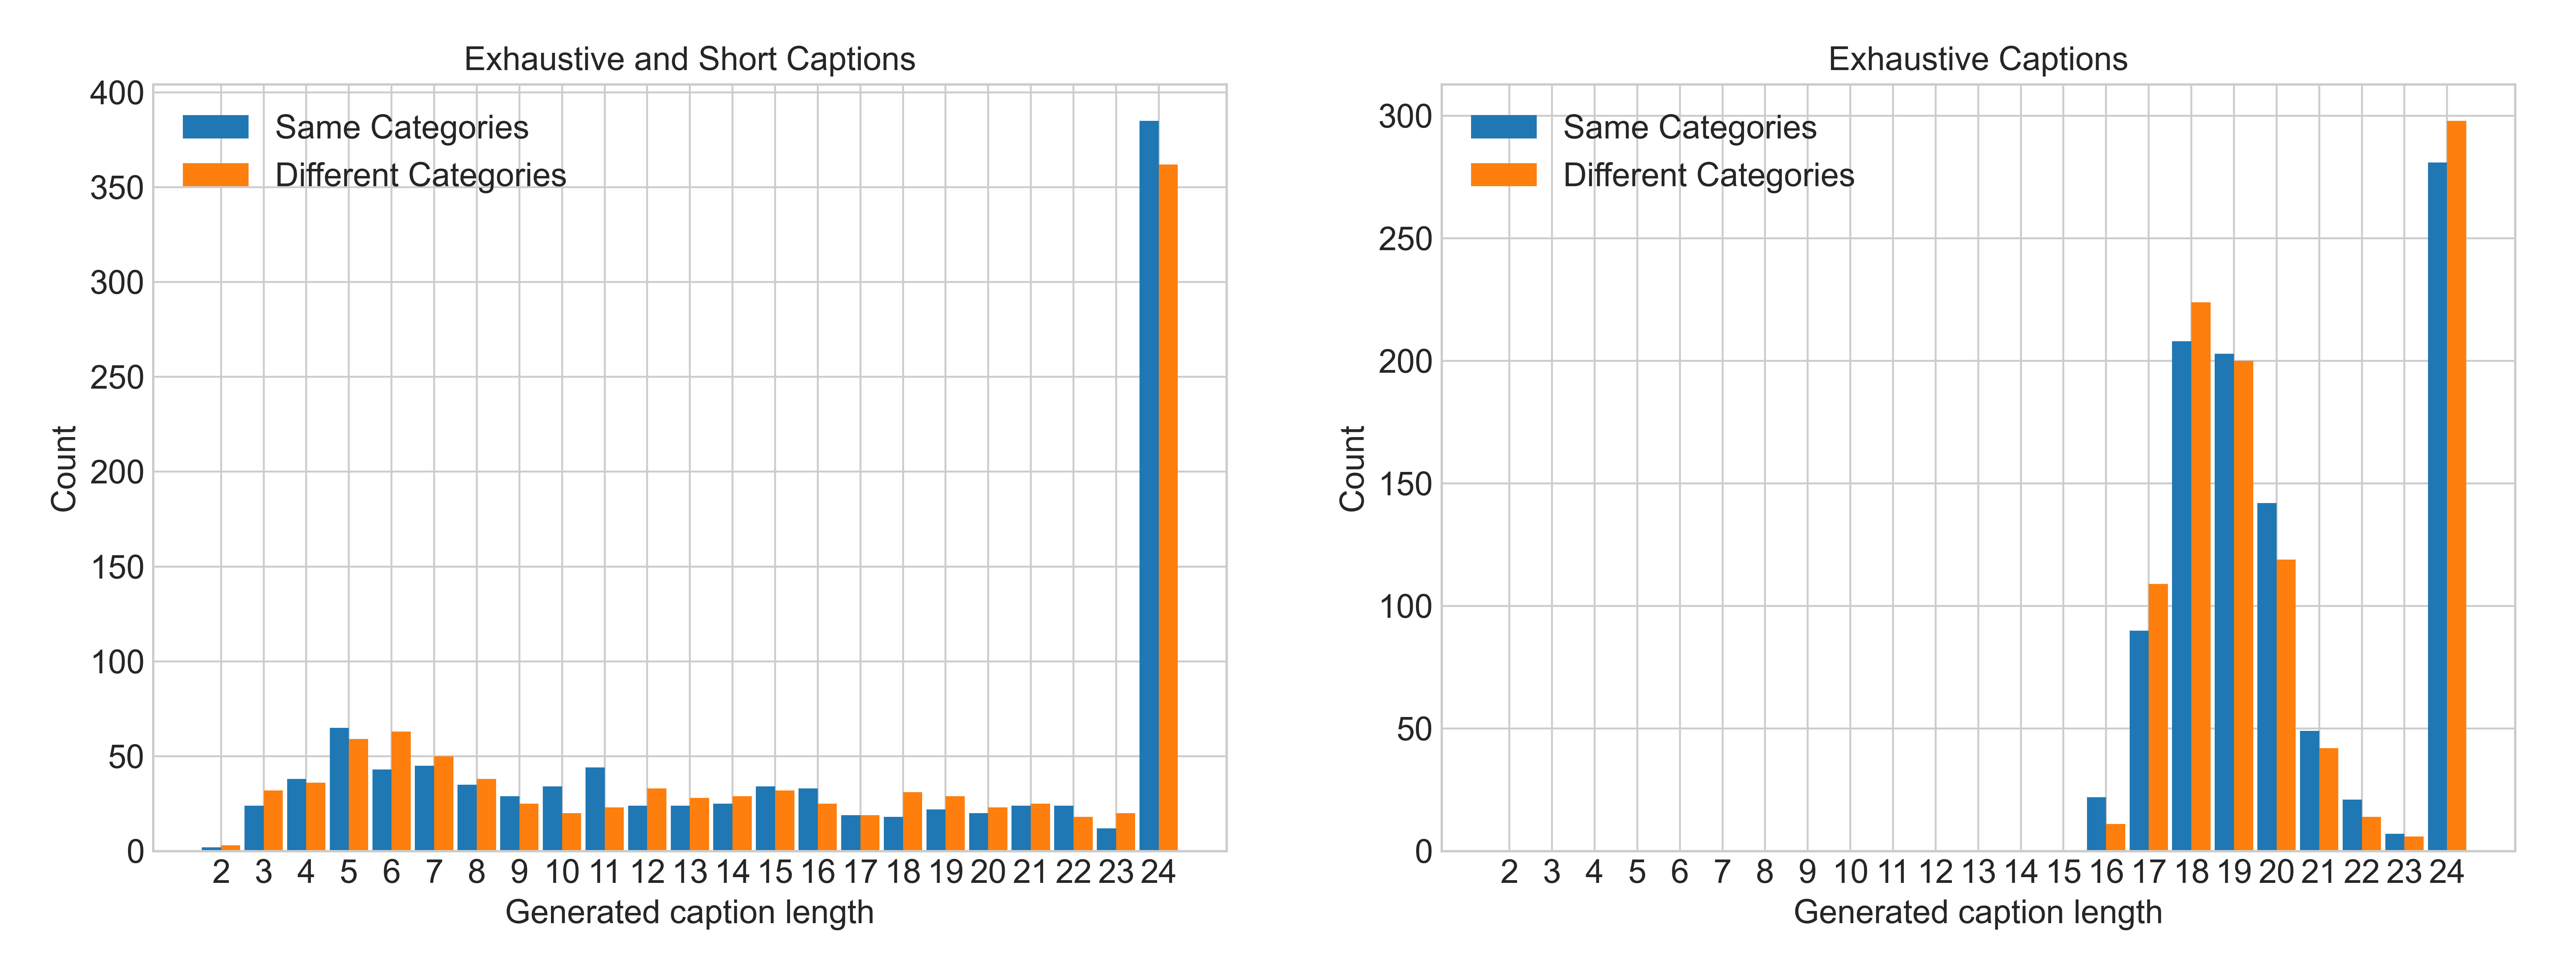
\includegraphics[width=\linewidth]{images/3dshapes_exh_short_similar_sameTest_diffTest_length_counts.png}
	\caption{Generated caption lengths for the mixed captions (left) and exhaustive (right) speakers trained in the similar pairs experiment on 3Dshapes. The test images were either similar along the same features as the training image pairs, or along the other three features.}
	\label{fig:3dshapes_exh_short_same_diff_lengths}
\end{figure}

\begin{figure}[h]
	\centering
	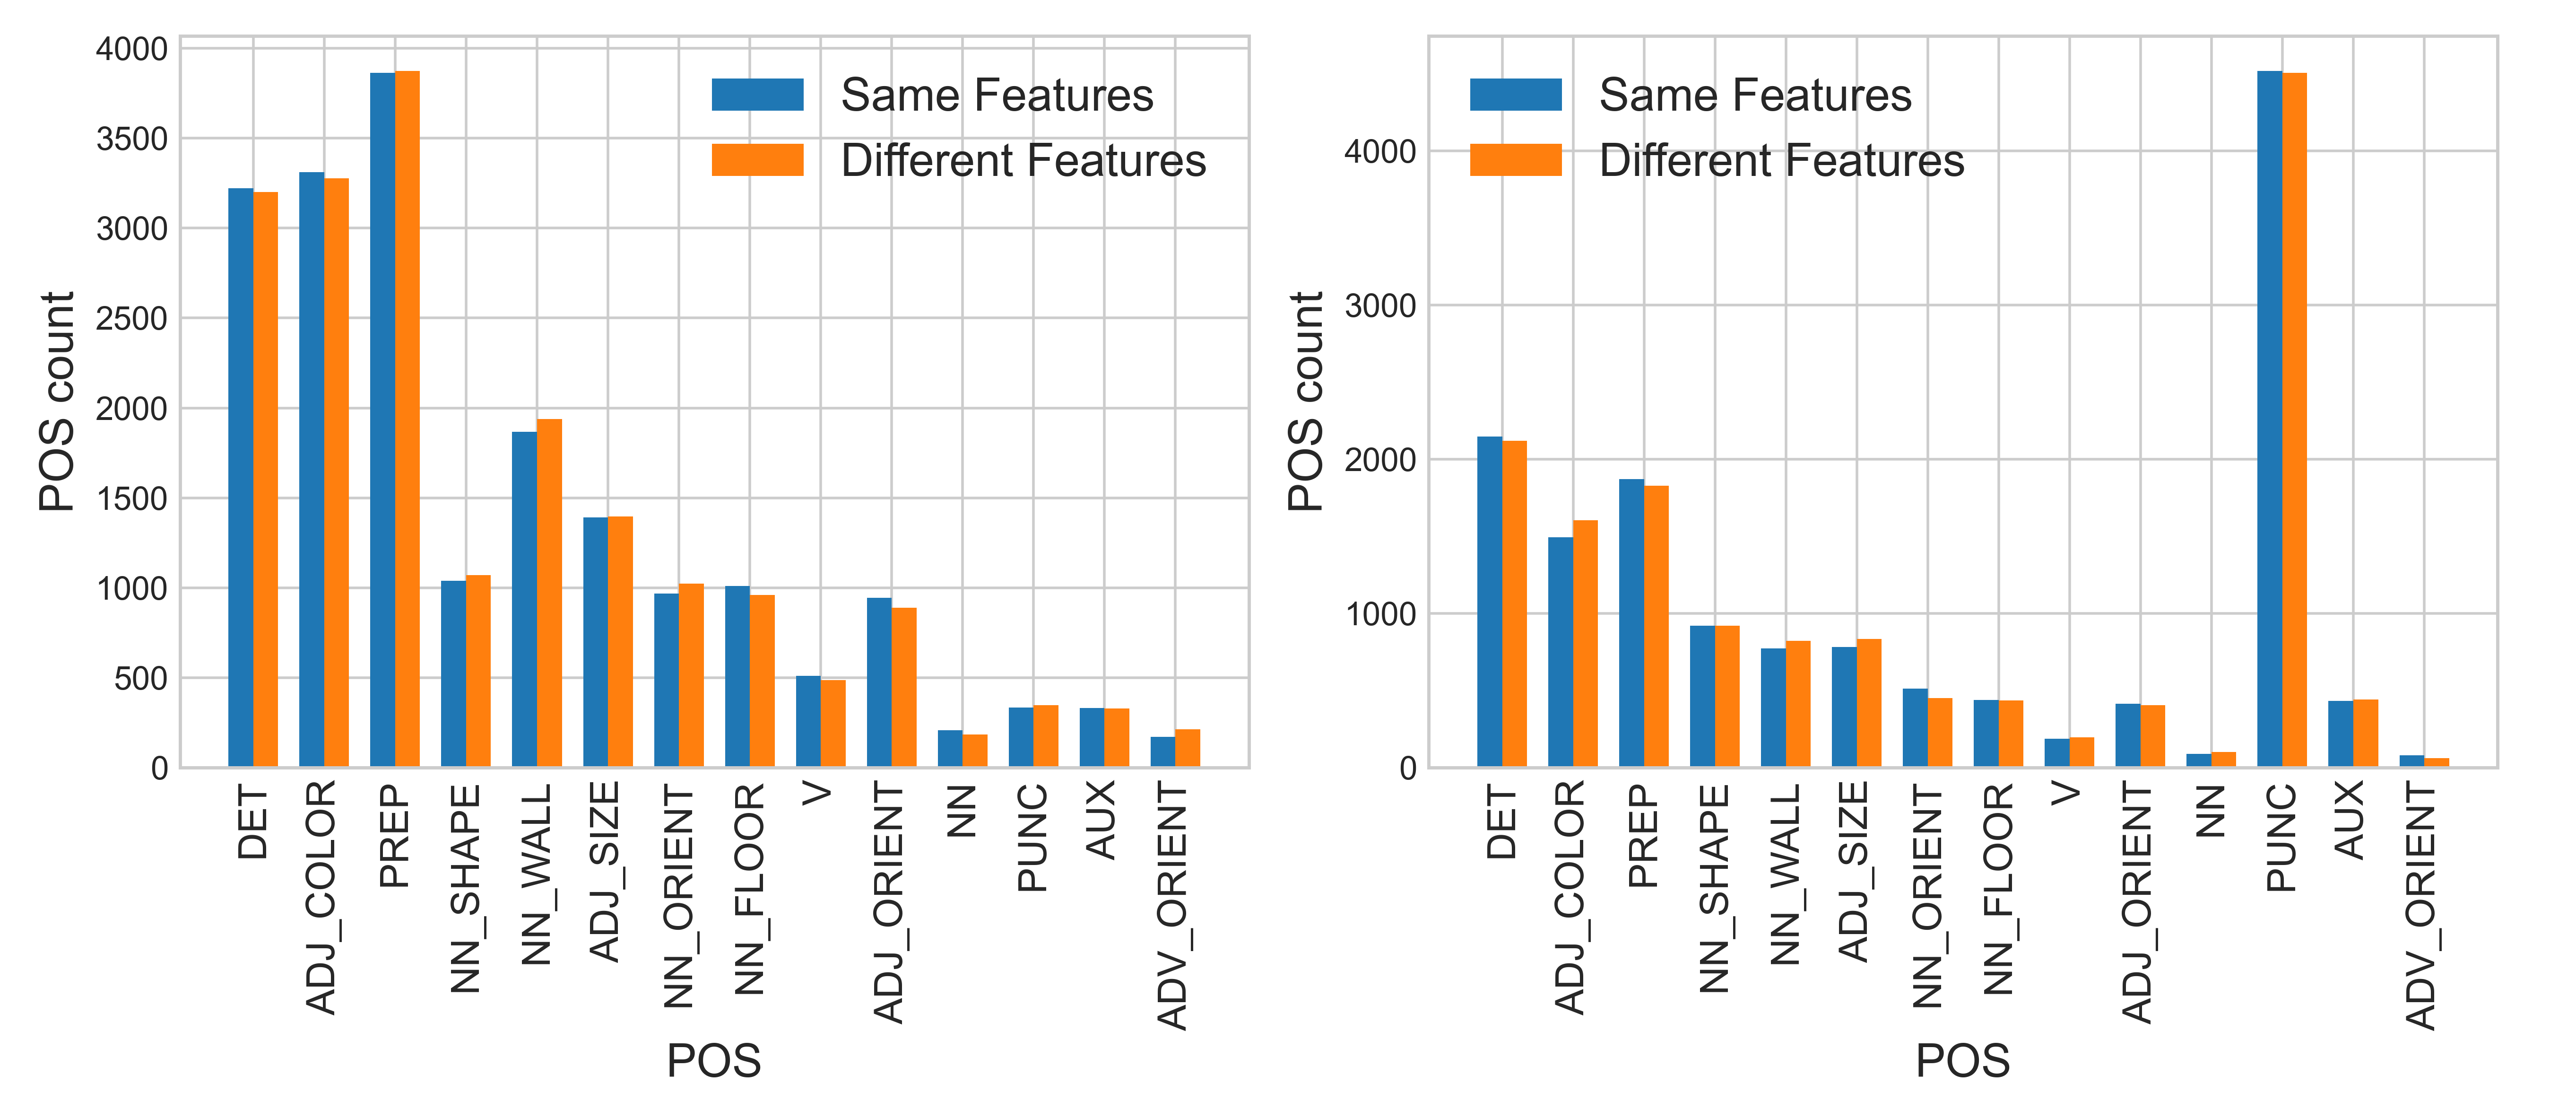
\includegraphics[width=\linewidth]{images/3dshapes_similarFixedPairs_exh_vs_short_sameTest_vs_diffTest_POS_counts.png}
	\caption{POS counts in captions produced by speakers trained on image pairs matching w. r. t. fixed features, tested on images matching on the same features (blue)~vs.~on different features (orange). Left: Speaker trained with exhaustive captions only. Right: Speaker trained with both short and exhaustive captions.}
	\label{fig:3dshapes_exh_short_same_diff_POS}
\end{figure}

In sum, this is a promising result showing that it may not be necessary to have completely exhaustive, almost task-specific, annotations for the agents to learn to flexibly adjust the length of their messages---they can be trained to do so via learning from interaction in variable visual contexts. However, more exhaustive captions are more advantageous for teaching the speakers to adapt their message granularity in response to contextual needs via mentioning different attributes, and not the message length.

%\begin{figure}
%	\centering
%	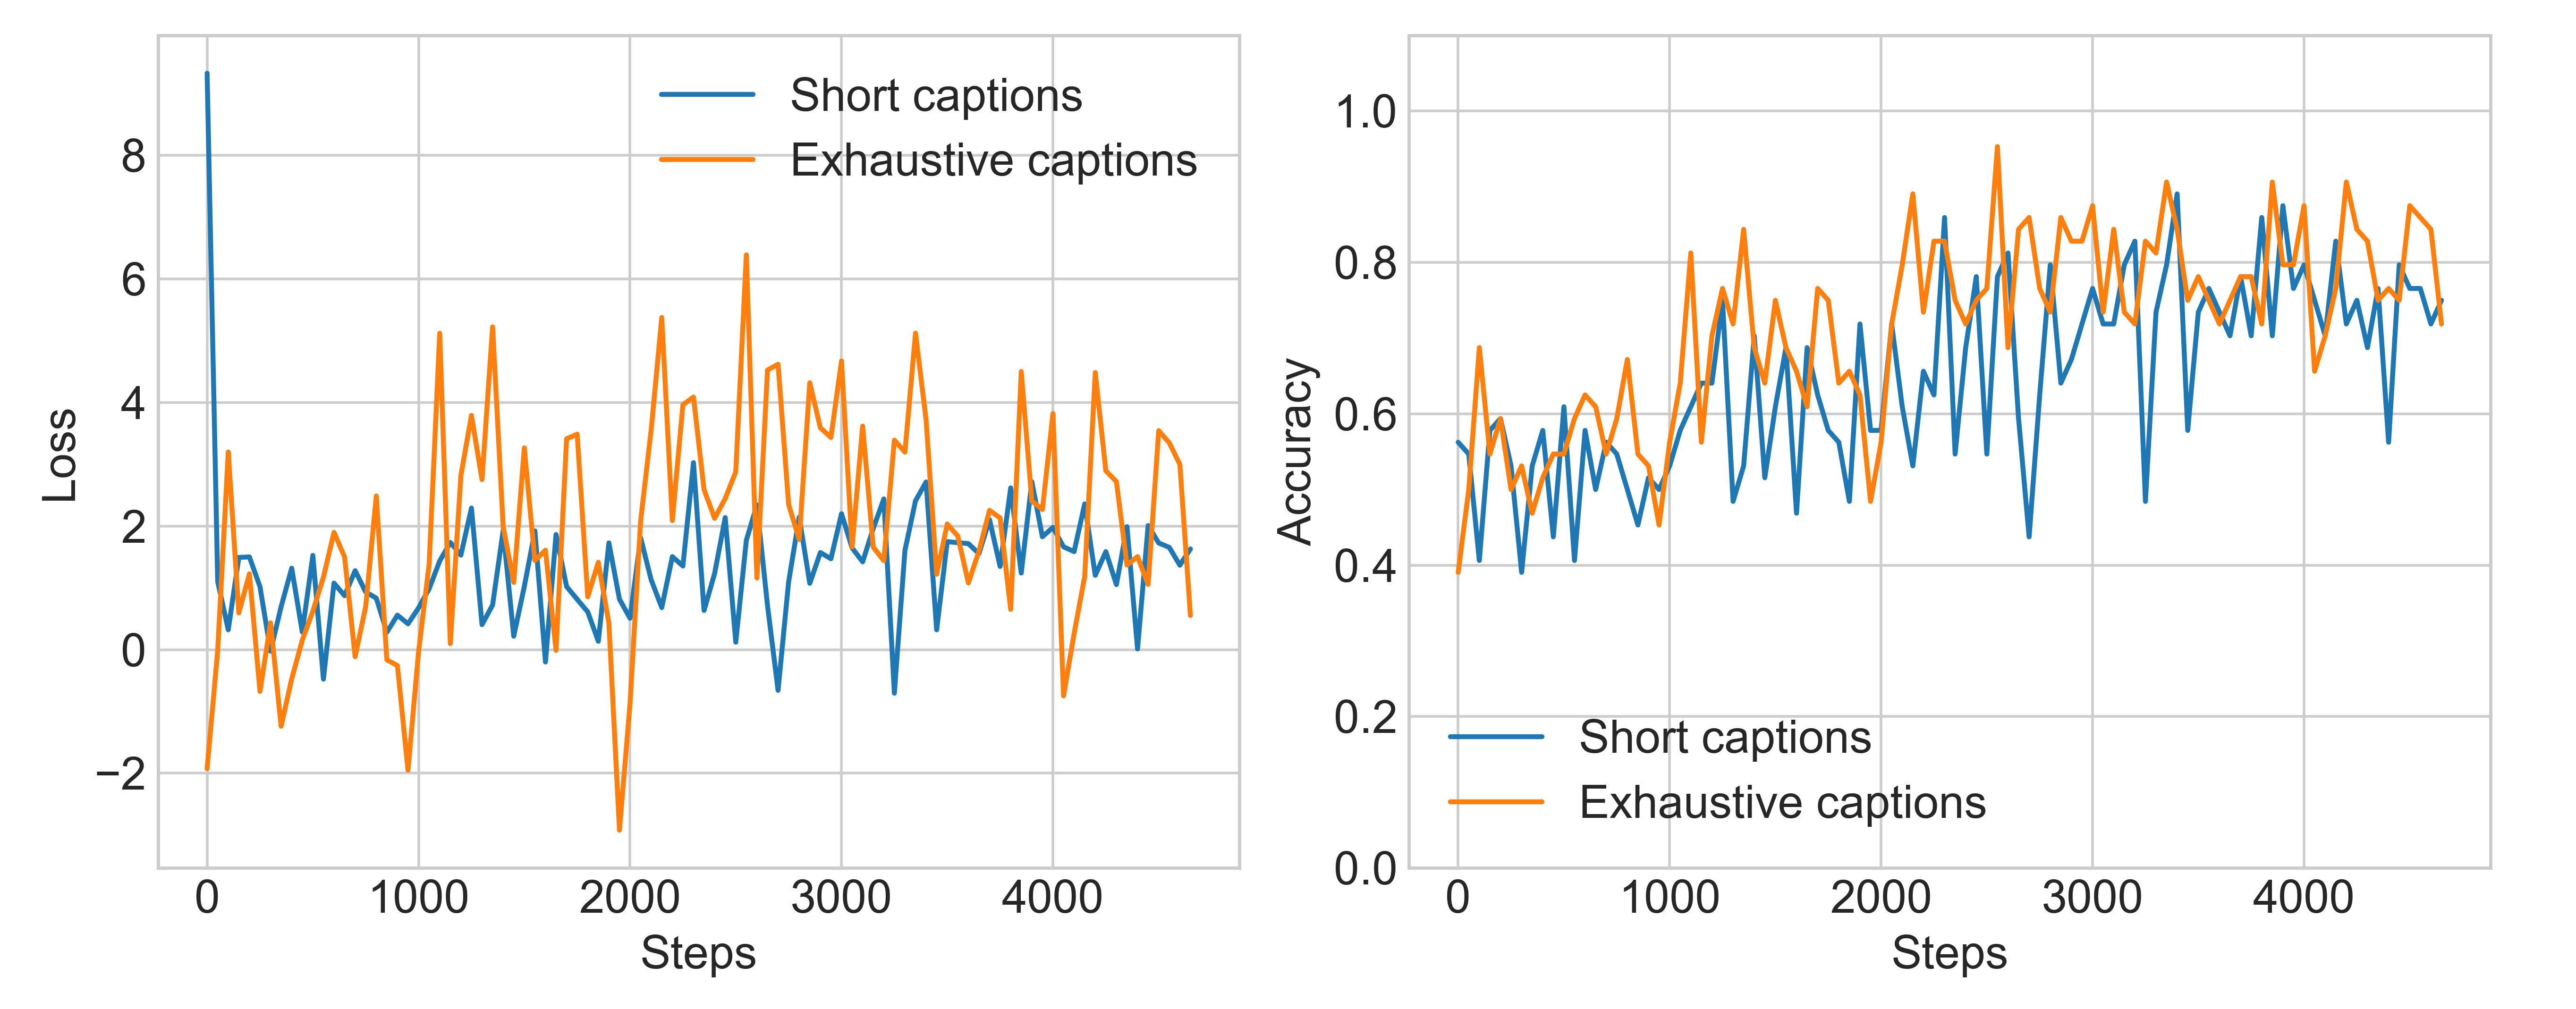
\includegraphics[width=\linewidth]{images/shapes_short_vs_exh_refgame_49_pure_075_similar.png}
%	\caption{Training dynamics on similar image pairs given a dataset with exhaustive captions vs. short captions only.}
%	\label{fig:3dshapes_short_v_exh_similar_losses}
%\end{figure}
%Given the strong effect of length, it does not come surprising that the structural drift of exhaustive captions is higher than of short ones. However, the semantic drift is much more severe for short captions, compared to exhaustive ones, therefore, at least partly supporting \textbf{H8}. 
%\begin{figure}
%	\centering
%	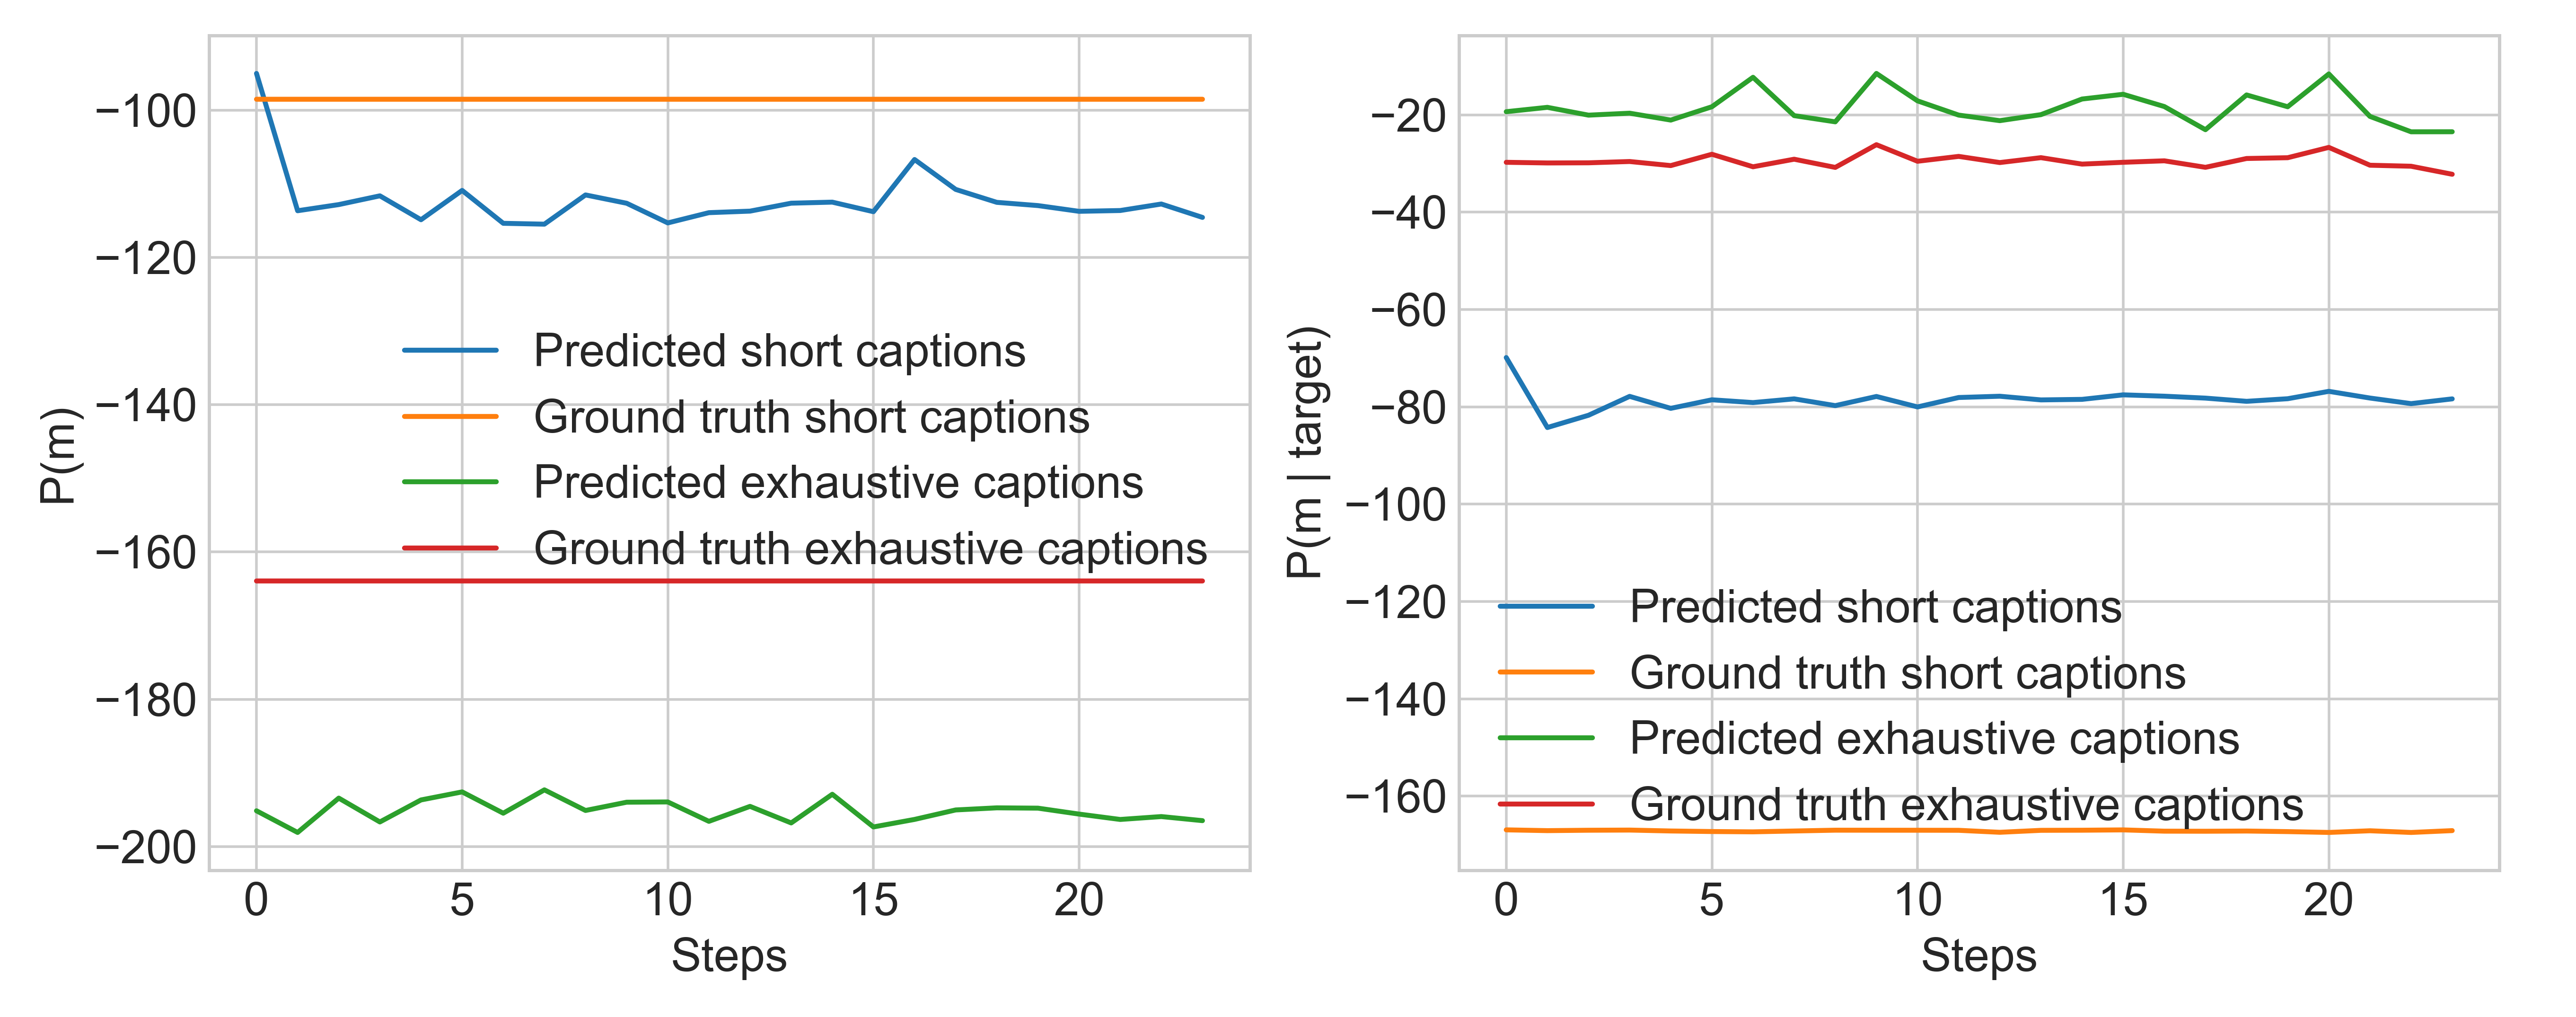
\includegraphics[width=\linewidth]{images/3dshapes_short_vs_exh_structural_semantic_drift_49_pure_075_similar.png}
%	\caption{Language drift metrics computed during training gieven model trained on similar image pairs given a dataset with exhaustive captions vs. short captions only. The drifts were computed on random image pairs for comparability.}
%	\label{fig:3dshapes_short_v_exh_similar_str_sem}
%\end{figure}
Summarizing the experiments on the 3Dshapes dataset, it was shown that the agents could successfully learn the reference game on this synthetic dataset. Crucially, thir success depended on the similarity of the image pairs. 
The agents were also subject to structural and semantic drift phenomena, although some dynamics differed from the observations in the literature and in the MS COCO experiments, revealing the importance of the nature of visual input, the captions and the action space size (i.e., the vocabulary size) for language drift. It was also shown that the magnitude of the drift metrics may be influenced by the nature of the dataset compared to the datasets used for training the models employed for computing the metrics. It was also shown that the success of fine-tuning the speaker for the task might be dependent on fine-grained differences in the visual input. 
It was shown that the presence of exhaustive annotations was not necessary in order to mitigate language drift, although it might help the speaker to learn to describe most discriminative attributes of the target in complex contexts. On the contrary, dataset statistics like the length of the captions which correlates with exhaustivity might play a larger role with respect to language drift than the exhaustive content of the annotations.

\section{Language Drift Hypotheses: Discussion}
\label{hypos_discussion}
Experiments described in the previous section addressed several hypotheses regarding language drift in multi-agent reference games and aimed to provide a comprehensive picture as to which factors might cause or influence the strength of different types of drift.
First, results are summarized with respect to the hypotheses (listed in Section~\ref{hypos}). Then a discussion by language drift type is provided. Quantitative statistical results are also provided for the hypotheses; depending on the particular hypothesis, Pearson's correlation coefficients, one-sample, two-sample or paired samples $t$-tests were computed. $\alpha=0.05$ is used as the significance level.\footnote{The normal distribution is assumed for the measures on which $t$-tests are computed.} The reported differences in drifts are in terms of log probabilities for structural and semantic drift, in terms of average numbers of tokens for discrete overlap, and in terms of cosine similarity differences for continuous overlap. \\
\newline
\textbf{H1:} Confirming expectations, structural drift increased in the baseline experiment on the MS COCO (Section \ref{expt:coco_baseline}) dataset. That is, the log probability under a pretrained LM of the messages generated by the speaker decreased after the agents learned to play the reference game, compared to the respective pretrained agent. Additionally to the original expectations, this was the case for all configurations of the structural loss weight. This was confirmed by a one-sample one-sided $t$-test ($t = -2.337, p = 0.040$). Structural drift was not as strong in the experiment on similar image pairs wherein the agents were also less successful, confirming that functional success was at least partly responsible for structural drift on MS COCO.
In contrast, the hypothesis was not borne out in the 3Dshapes dataset random pairs experiments (Section \ref{expt:3dshapes_baseline}) compared to the pretrained speaker ($t = -1.158, p = 0.156$). It was also not the case for similar pairs.% ($t = -0.457, p = 0.339$)
These results indicate that structural constraints might be more effective when the speaker needs to learn a smaller vocabulary like the 3Dshapes one, compared to MS COCO. However, the size of the vocabulary is intertwined with differences in perceptual nature of the images, which might have influenced the strength of the functional training signal and the naturalness of the messages, and, therefore, the trade-off with the structural signal.\newline
\textbf{H2:} In line with the hypothesized effect, semantic drift was stronger in the baseline experiment on MS COCO compared to the pretrained speaker (Section \ref{expt:coco_baseline}). That is, the conditional log probability of the generated messages given the target under the pretrained speaker model decreased. The drift was also higher for the experiments with $\lambda_s=0$, $\lambda_s=0.25, \lambda_s=0.5, \lambda_s=1$. Overall, the drift was significantly higher in the random pairs experiments compared to the pretrained speaker ($t = -3.484, p = 0.013$).
The drift was also increasing during training on similar image pairs, hinting at more likely speaker-listener co-adaptation when the discriminative task was more difficult.
In line with expectations, semantic drift in the baseline 3Dshapes experiment was higher compared to the pretrained speaker (Section \ref{expt:3dshapes_baseline}). It was additionally the case for the $\lambda_s=0$ experiment only, such that, overall, semantic drift was not significant in the random pairs experiments ($t = 1.043, p = 0.822$). No large drift increases were observed in the similar pairs experiments ($t=1.241, p= 0.849$). 
In sum, confirming expectations, semantic drift was observed rather consistently in the baseline experiments on both datasets.\newline
\textbf{H3:} The expectation was that, as the speaker learned to play the reference game, the overlap metrics increase, reflecting that the messages become more discriminative. Against expectations, the overlap metrics decreased on all experiments compared to the overlaps of the ground truth captions, indicating that, at least on the surface, the difference between the produced messages and their contrast with target versus distractor descriptions decreased, compared to the original difference between the target and distractor ground truth captions. For MS COCO, the discrete overlap was also lower for the baseline experiments than for the pretrained speaker, except for the $\lambda_s = 0$ and $\lambda_s = 0.75$ configurations (Section \ref{expt:coco_baseline}). The continuous overlap was higher than for the pretrained speaker only for the $\lambda_s = 0.25$ configuration. This indicates that some configurations were subject to functional drift, and only in a few experiments did the speaker manage to learn more discriminative captions than during pretraining (one-sample one-sided $t$-test: increasing discrete overlap in random pairs: $t = -0.847, p =0.778$, increasing continuous overlap in random pairs: $t = -1.633, p = 0.911$).
On 3Dshapes, the discrete overlap was lower on all random pairs experiments than for the pretrained speaker ($t = 4.171, p = 0.993$ for an increase in overlap). The continuous overlap was lower in all configurations except for $\lambda_s=0.5$ (Section \ref{expt:3dshapes_baseline}, $t = -1.897, p = 0.935$). The overlaps increased only on similar image pairs, indicating that this speaker might have learned more discriminative messages under more complex visual input.
However, in general, the fact that the overlaps \emph{de}creased may not necessarily be indicative of bad discriminative performance. More specifically, the low discrete overlap value might be due to the fact that the generated captions contained words which were not part of the ground truth caption because, for instance, they referred to features which were not mentioned in the descriptive ground truth captions, but were chosen under discriminative pressure by the trained speaker.\footnote{Thanks to Malte Heyen for the discussion which led to this point.} 
In sum, the data did not provide evidence that the overlap consistently increased as the speakers learned the reference game, indicating that even when the agents succeeded in the reference game in terms of accuracy, they still may have been subject to functional drift from the perspective of human interlocutors.\newline
\textbf{H4:} This hypothesis concerned the strength of the structural constraints during training; it was expected that with increasing structural regularization strength (i.e., structural loss weight), structural and semantic drift would decrease, for both datasets. Varying the structural loss weight on MS COCO (Section \ref{expt:coco_baseline}), it was observed that the structural drift significantly decreased with \textit{de}creasing structural loss pressure ($R^2 = -0.955, p = 0.011$).\footnote{The Pearson correlation coefficient was computed on the mean validation drift values and structural weights.} Semantic drift also significantly decreased as the structural loss weight decreased ($R^2 = -0.934, p =0.020$). For 3Dshapes (Section \ref{expt:3dshapes_baseline}), structural drift seemed to slightly decrease with increasing structural contraints, but the trend was negligible ($R^2=0.028, p = 0.964$). By contrast, semantic drift decrease with increasing structural weights was more pronounced ($R^2 = 0.519, p = 0.371$). To sum up, the hypothesis was somewhat supported by the data on semantic drift in the 3Dshapes exeriments, but not for other aspects. That is, contrary to expectations, language drift was not consistently mitigated by stronger structural constraints, indicating that the reason for language drift might not be the lack of supervision, at least for agents acting in a large action space like the MS COCO vocabulary. \newline
\textbf{H5:} For this hypothesis, the increase in the overlap metrics was expected to be smaller when comparing the pretrained speaker to the speaker trained on similar image pairs, than when comparing the pretrained speaker to the speaker trained on random image pairs. This was expected for both datasets. First, results for discrete overlap are discussed. 
For MS COCO, the increase was 0.003 on baseline random pairs and the value decreased by 1.039 on similar pairs, in favor of the hypothesis (Sections \ref{expt:coco_baseline} and \ref{expt:coco_similar_pairs}). 
For 3Dshapes, the overlap decreased by 0.181 for baseline random pairs. For the fixed features similar pairs with exhaustive captions, when tested on the same test set, it decreased by 2.553. When tested on the different test set it decreased by 3.357 (Section \ref{expt:3dsapes_similar}). Turning to the mixed lengths speaker (Section \ref{expt:3dshapes_short}), the overlap increased by 0.007 on random pairs and decreased on similar pairs (by 1.472 and 0.394, respectively, when tested on same and different test sets). Quantitatively, the overlap difference was only close to significance (two-sample two-sided $t$-test, $t= 2.402, p = 0.053$)
Turning to continuous overlap, on MS COCO, the similar pairs overlap increased by 0.001 compared to the increase on random pairs. For 3Dshapes, the overlap decreased compared to the pretrained model on all similar pairs tests, while the random pairs overlap only decreased by 0.001 on mixed length captions ($t=0.876, p=0.430$).
Therefore, in sum, the premise of the hypothesis that the overlap metrics increase after training on the reference game was not supported by the data across the board. It was only the case for discrete overlap of the baseline random pairs MS COCO and mixed captions 3Dshapes baselines, and continuous overlap on MS COCO similar pairs. The other speakers' productions' overlaps decreased. However, in relative comparison, this speaks in support of the hypothesis, as even for the exhaustive 3Dshapes experiments, the decrease in discrete overlap on similar pairs was much stronger than on random pairs. This decrease was also much stronger for continuous overlap. 
Further, looking at the different magnitudes of the discrete overlap values in the exhaustive and mixed caption results on 3Dshapes, it is apparent that this metric reflects the average lengths of ground truth and generated captions.
Nonetheless, it appears to capture functional drift as increasing difficulty of completing the referential task, because the values were, on average, lower whenever the agents' accuracy was lower, and it reflected contextual difficulty of the task. For more tangible results regarding the continuous overlap metric, longer training of the embedding layers might be necessary.
%In sum, the discrete overlap may be considered a valid functional drift metric.
The second part of the hypothesis regarding message length and specificity increasing in presence of more difficult image pairs was supported by small trends in the similar pairs experiments on both datasets. More specifically, the speakers increased their message length when communicating about targets in more difficult context for both datasets. Speakers in the 3Dshapes experiments additionally were able to refer to more specific target attributes. These findings complement the POS analysis in \cite{lee2019countering} by pitting against each other the productions of agents trained in different conditions and thereby qualitatively investigating the effects of these conditions. In sum, the speakers were shown to be able to flexibly adjust the granularity of their messages, when environmental pressure was sufficient.\newline
\textbf{H6:} Under this hypothesis, the mitigation of drift by removing the potential for speaker-listener co-adaptation was considered. Confirming expectations, structural and semantic drifts were smaller when the speakers were trained against a fixed listener, compared to the jointly trained listeners (Sections \ref{exp:coco_fixed_listener} and \ref{expt:3dshapes_fixed}). More precisely, semantic drift was smaller for fixed listener experiments for both datasets and both structural loss weight configurations; however, the differences were not significant (paired-sample one-sided $t$-test,  3Dshapes: $t = 3.746, p = 0.083$; MS COCO: $t = 1.825, p =0.160$).\footnote{This hypothesis is the only one containing comparisons where the grouping variable is only $\lambda_s$ and not the experiment type. Therefore, paired-sample tests are only run here.} Qualitatively, this was also the case for all structural drifts except for the $\lambda_s = 0$ configuration on 3Dshapes, where the drift was lower with the jointly trained listener (3Dshapes: $t=-0.156, p=0.549$;  MS COCO: $t = 11.729, p =0.027$). Confirming results from the literature \parencite{lazaridou2020multi}, it is visible that the fixed listener was effective in keeping the grounding of the language more constant and thereby alleviating semantic drift. Extending beyond previous results, it even somewhat mitigated the structural drift, possibly by implicitly enhancing the structural training signal with the help of the listener pretrained on ground truth captions.\newline
\textbf{H7:} This hypothesis posited that the difference in the structural drift between speakers fine-tuned in reference games and the pretrained speakers is smaller for the 3Dshapes experiments, compared to the difference of the MS COCO experiments.
Those differences are compared one by one (3Dshapes~vs.~MS COCO) in the following. The average differences in the baseline experiments with varying structural loss weights were 0.340 and 2.824 worse than pretrained speakers (Section \ref{expt:3dshapes_baseline} and Section \ref{expt:coco_baseline}). In the similar pairs experiments (with exhaustive captions on 3Dshapes), they were on average 0.603 and 1.495 worse than pretrained speakers ( Section \ref{expt:3dsapes_similar} and Section \ref{expt:coco_similar_pairs}); for the fixed listener experiments, they were 0.203 better than pretrained speakers for 3Dshapes and 0.918 worse on MS COCO (Section \ref{expt:3dshapes_fixed} and Section \ref{exp:coco_fixed_listener}). However, the two-sample $t$-test revealed that this difference was not significant ($t=2.449, p=0.07$).
That is, at least qualitatively, across the different types of experiments the data supports the hypothesis, indicating that the presence of exhaustive captions during training helped alleviating structural drift. These results are also consistent with the interpretation that the speakers on MS COCO might resort to structural drift as a strategy for higher task success, in absence of sufficiently exhaustive annotations.
An additional potential source of the difference between the experiments remains, however, the different nature of the images (synthetically generated geometric shapes versus real photos) and the difference in the vocabulary sizes the speakers learned (49 tokens versus 4054 tokens). \newline
\textbf{H8:} Following up on the potential confound in the last hypothesis, it was hypothesized that the structural drift is higher for mixed caption experiments compared to exhaustive caption experiments, on all pairs, as measured by the difference in structural drift between baseline, similar pairs and respective pretrained speakers. This expectation was based on the intuition that under a lack of descriptive words, the speaker may resort to structural drift as a strategy for discriminative communication. Furthermore, combined with expectations formulated in \textbf{H5}, increasing the difficulty of the referential task by using similar pairs, it was expected that this difference between exhaustive and mixed caption speakers increases. 
Comparing the baseline experiments on random pairs (Section \ref{expt:3dshapes_baseline}~vs.~Section \ref{expt:3dshapes_short}), this hypothesis was not supported by the data, as the structural drift of the mixed lengths baseline speaker improved compared to the pretrained mixed lengths speaker by 3.623, while the structural drift of the exhaustive baseline speaker almost did not change compared to pretrained exhaustive speaker (it improved by 0.255). %Comparing structural drifts of these speakers on similar pairs experiments wherein the pairs matched on random features, the exhaustive speaker exhibited structural drift compared to the pretrained one (Section~\ref{expt:3dsapes_similar}). \pt{The comparable experiment on mixed captions is missing}. 
Comparing structural drifts of the exhaustive speaker on similar pairs which matched on fixed features, the drift decreased compared to the pretrained speaker by 2.044 (same test) and 2.229 (different test). For the mixed captions speaker (Section~\ref{expt:3dshapes_short}), the drift increased compared to the pretrained speaker by 0.1 (same test), and decreased by 5.190 compared to pretrained speaker when tested in the different features test set, providing no consistent support for the hypothesis (two-sample one-sided $t$-test: $t=2.415, p=0.963$). Taken together, these results indicate that the speaker did not resort to structural drift as a strategy for more successful discriminative communication because of a lack of appropriate descriptive words. She did not do so even given similar target-distractor pairs which called for more fine-grained discriminative messages. Therefore, one might hypothesize that structural drift is generally rather an artifact of a lack of an appropriate training signal rather than some type of the agent's strategic loophole behavior, and is considerably influenced by message lengths, mitigated by more stable training of the RNN based speaker on shorter captions.
\newline

Taken together, these results provide an extensive overview of different factors which may influence language drift. Summing up by drift type, it was found that \textbf{structural drift} was best mitigated by the presence of exhaustive captions in the training set, sampled from a not too large action space, and it was dependent on the distribution of lengths of the training sentences. The drift was generally lower for speakers trained to produce shorter messages. For \textbf{semantic drift}, it was found that it was mostly due to speaker-listener co-adaptation, as was shown by the mitigation provided by the fixed listener. Additionally, it was found that semantic drift was much lower when the speaker was trained also on short captions, indicating that grounding was easier to learn from shorter sequences. That is, statistics of the dataset had a large impact on structural and semantic drifts, which, in fact, was even larger in the presented experiments than content-related aspects like exhaustivity or the complexity of the scenes or image pairs. However, it was also shown that these drifts are less likely to occur when the functional training signal is weak. Finally, \textbf{functional drift} measures also reflected the average ground truth caption length, being lower when the image annotations contained short captions (3Dshapes dataset). Furthermore, crucially, the discrete metric captured the complexity of the referential task, decreasing when the referential task was more complex (like in the similar pairs experiments).
Comparing this decrease with the dynamics of test accuracy, it can be seen that the discrete overlap metric was indicative of the test accuracy, making it a valid task-functional metric which, importantly, can be computed \emph{without} human data from the same task. Functional drift could be counteracted by using the baseline configuration with random image pairs on MS COCO, and with mixed-length captions on 3Dshapes, although the improvements were rather small. Instead, the experiments showed which factors worsened functional drift---namely, the conceptual and perceptual similarity of target and distractors, as well as communication via long messages (longer than 15 tokens). The results were generally more pronounced for discrete overlap, suggesting that this surface form based metric might be more appropriate for reference games involving natural language when the task fine-tuning phase is rather short. 
Summing up, the results allow to conclude that the functional training signal should be prominent enough in order to achieve optimal task-conditional fine-tuning of the speaker, and training on the task should proceed for sufficiently long.

In conclusion, the experiments have revealed how strong the effect of the speaker's pretraining and decoding strategy is on the downstream reference game performance, and how these effects enter into fine-grained interactions with the environment of the reference game, including its aspects like the nature of the target-distractor pairs, training duration and the length of the available annotations. Critically, the results showed that language drift is better mitigated when the agents have to learn a smaller action space, as it was the case for 3Dshapes, compared to MS COCO. Thus, this calls for much closer attention to training and architectural details in multi-agent communication experiments than is common in the literature.
% Fixed listener results consistent with \cite{lazaridou2020multi}.

\chapter{Discussion}
\label{chapter06}
Communicating about the ever-changing world around us in a context-appropriate way is a fascinating human ability. Yet training artificial neural agents to communicate in the same way is a non-trivial task. This thesis set out to investigate how this task can be approached by training artificial agents to use natural language in order to communicate about realistic images in a multi-agent communication setting. More specifically, the agents were trained to play a \emph{reference game} in which they had to produce maximally \emph{discriminative} messages in order to succeed on the task. Importantly, extending beyond previous work, the agents both communicated in natural language and received visual input in form of real-world photos. Building upon the work by \cite{lazaridou2020multi}, the phenomenon of \emph{language drift} which occurs as agents improve on their task was the main focus of this work. Aiming to measure the degree of language drift and explain its potential sources, various reference game experiments with different configurations were conducted. 

This final chapter concludes the thesis by, first, discussing results and limitations of the presented experiments and outlining potential directions for future studies. Then, present work is put in context of multi-agent communication research as well as cognitive science, in general, before closing with a conclusion. 

\section{Experiments}

Various experiments were conducted in this thesis in order to investigate language drift in reference games. The main experiments wherein agents were trained to communicate about realistic visual input in natural language were conducted on the MS COCO Captions dataset \parencite{chen2015microsoft}. All reference games included two agents, a speaker and a listener, who communicated about pairs of images (i.e., a target in context of one distractor).
First, a baseline experiment established that agents trained with a combination of a task-based functional learning signal and a language structure preserving supervision signal can successfully learn to play the reference game on real-world images. Second, a set of experiments varying the strength of the supervision constraints put on the surface structure of the messages the agent produced showed that this learning contraint did not affect the strength of the language drift. Third, in contrast to preceding experiments where the target and the distractor image were combined at random, an experiment with \emph{similar} target-distractor pairs was conducted. It revelaed that it was much more difficult for the agent to learn the task given images which were difficult to discriminate, confirming the agents' sensitivity to their communicative context. It also showed that in absence of a strong task success based learing signal, language drift was weaker. Finally, in order to address the potential effect of speaker-listener co-adaptation, experiments wherein the speaker was trained against a fixed pretrained listener were conducted. They showed that the functional improvements visible in the previous experiments are to a large extent carried by this co-adaptation; they also showed that, consistent with intuitions, the grounded listener mitigated semantic drift.

In order to investigate the importance of the presence of fully discriptive, or, exhaustive example captions in the training dataset, the results from MS COCO experiments were compared to experiments on a different dataset---the 3Dshapes dataset \parencite{burgess20183d}. To this end, custom natural language annotations were created for this dataset. Two sets of annotations were created---exhaustive image captions describing all six properties that varied between the images in the dataset, and short image captions which mentioned only up to three properties of the image.
The same experiments as on MS COCO were replicated on this dataset with exhaustive annotations. The qualitative results of these experiments patterened with MS COCO, although, on average, language drift of the agents trained on the reference games compared to pretrained speakers was smaller relative to MS COCO, indicating that exhaustive annotations of the 3Dshapes mitigate drift. However, this comparison was confounded with a large difference in the vocabulary sizes the agents learned. 
Therefore, an additional experiment varying the exhaustivity within the 3Dshapes dataset were conducted, including annotations consisting of both exhaustive and short captions. It showed that agents were still able to learn the reference game, and language drift actually decreased, indicating that the shorter annotations were enough for identifying discriminative properties of the images and that shorter messages were easier to learn for the speaker. Finally, in order to investigate if the need for exhaustive captions is stronger when target and distractor are more difficult to distinguish (i.e., the pairs are similar), the similar pairs experiment was also conducted with annotations including short captions. The results did not differ from the experiments with fully exhaustive annotations in terms of game success, while language drift also decreased, indicating that shorter messsages were easier to learn even given more complex visual input. Nevertheless, a POS analysis revealed that exhaustive annotations might be critical for learning to address discriminative features of the images more precisely.

However, present experiments were subject to some limitations which should be improved upon in future work. First, due to computational constraints all reference games were only trained for two epochs (around 4,800 steps), which might have led to an absence of full effects of the task-based training signal \parencite[compared to, e.g.,][who had 300,000 training steps]{lee2019countering}. Longer training might provide results which can be interpreted more strongly with respect to the influence of the functional training signal. In particular, longer training might allow to better estimate the validity of the continuous overlap measure as a functional drift metric (cf. Section~\ref{hypos_discussion}).
Second, due to the general difficulty of training image captioning models which generalize well to the auto-regressive inference mode \parencite{lamb2016professor}, and the large space of hyperparameters which may be tuned for training such a model, the quality of the pretrained speaker models was not comparable to state-of-the-art image captioners (see Table \ref{tab_coco_metrics_ref}~vs.~Table \ref{coco_grid_searches_speaker_pretrain}). This might have led to overly pessimistic structural drift estimates which are computed under a pretrained LM and, therefore, measure the naturalness of the produced captions. Although the relative comparisons between experimental configurations are not affected by this shortcoming because they were all based on the same pretrained speaker, replicating these results with a better base model could improve the comparability of the presented results to other image captioning work. To this end, alternative pretraining schedules like professor-forcing could be considered \parencite{lamb2016professor}. Furthermore, it could be explored whether starting with the auto-regressive pretraining mode and then increasingly transitioning to teacher-forcing might yield more stable model performance \parencite[although similar explorations by][suggest that this order might not work very well]{lowe2020interaction}. A pretraining strategy for the 3Dshapes dataset could also be determined separately because presented experiments used a strategy selected based on MS COCO performance. Different annotations for the 3Dshapes (e. g., with different syntactic structures) could also provide a broader picture of structural drift.
Third, all main experiments used pure decoding for sampling the speaker's messages; however, initial exploratory experiments showed that the decoding strategy might have a substantial influence on the task success (see~Appendix \ref{app:grid_search}), so future experiments should also consider other strategies like the popular beam search (see Section \ref{model_pretraining}). Furthermore, a speaker pretrained with greedy decoding should be employed to replicate and extend the presented greedy decoding experiments.
Finally, the embedding layer converting the natural language captions to vectorized representations were trained from scratch in all experiments. While this set up provided the advantage of creating embeddings optimal for the task, it substantially increased the number of learnable parameters of the model and, therefore, the complexity of the computational task. In order to alleviate that, future work should examine if the use of pretrained embeddings is advantageous \parencite[following, e.~g.,][]{atliha2021pretrained}.

Turning to the overall experimental set up, an interesting direction for future work might be to explore the effects of a larger number of distractors on the strength of language drift. Intuitively, the more distractors there are, and the more similar they are, the more constrained the functional learning signal might be, so that structural and semantic language drifts might be mitigated. However, this might lead to higher functional drift. Furthermore, training a population of agents (e.~g., a single speaker against a population of listeners, or a population with switching roles akin to \cite{bouchacourt2019miss}) would be an interesting future step with potential to uncover the dynamics of language drift in a population, which might connect to the line of work on language evolution in multi-agent communication \parencite[e.~g.,][]{graesser2019emergent, chaabouni2019anti, kirby2014iterated}. Note that the fixed listener experiments in this work approximate training a single speaker against an infinite population of listeners which in the limit converge to a single agent. Nonetheless, other fixed listener architectures may be considered. For instance, the listener could be an RSA-style literal listener agent interpreting the speaker's messages according to their probability given each of the images, as assigned by the pretrained speaker model (i.e., the listener's representation of literal semantics) \parencite[cf.][]{frank2016rational}.\footnote{This architecture was suggested by Michael Franke during the conceptualization of this thesis. It was explored for both datasets and did not yield successful reference games due to insuffiecient speaker quality.} 

Additionally, the experimental set up could be enriched by a text-to-image model in order to formalize functional drift through the lens of \emph{recoverability}---i.e., being able to reconstruct the intended image given the produced caption. The idea would be that discriminative captions have a higher recoverability measure for the target compared to distractors. For instance, this could be operationalized in two ways. One architecture could include a pretrained image-text retrieval model like VSE++ \parencite{faghri2017vse++}; this model would provide a top-k recall score which indicates how often the target is recovered as being among the top k most suitable image given a caption. This score is expected to be higher for that target than distractors, given discriminative messages. Alternatively, this could be operationalized via a generative text-to-image model like DALL-E\footnote{\url{https://openai.com/dall-e-2/}}, where, ideally, the image produced from the generated caption would be more similar to the original target than the distractor image. The recall score or the similarity metric could then be a functional drift measure. However, these metrics would both heavily depend on the nature of the pretrained models as well as in the chosen image similarity metric. Nevertheless, this might be a promising direction for future work which might resonate with cognitive aspects of communication (see Section~\ref{discussion_cog_perspective} below). 

Last but not least, follow-up experiments might consider alternative functional learning signal formulations. The presented experiments exhibited quite a large variance of the speaker loss component computed with the REINFORCE algorithm. Therefore, either baseline subtraction could be included (see Section \ref{rl_methods}), or the functional signal could be formalized with the straight-through Gumbel-Softmax estimator, as proposed by \cite{havrylov2017emergence}. They note that this might improve convergence for a larger action space (i.e., for the MS COCO experiments' vocabulary) and thus make the task-based training signal more pronounced, better isolating the signal necessary for learning discriminative language use.
%My architecture, esp for MS COCO, can essentially be interpreted as just show-casing that you can ground a second (receiver) agent against a pretrained image captioner. It is hard to consider this a multi-agent communication result since the effect or reinforce propagating the functional signal is so marginal. 

In general, the results indicate that multi-agent communication systems can be applied in realistic environments, yet the quality of their language is strongly affected by architectural considerations like the speaker pretraining mode which are often glossed over in the literature, as well as by the similarity of potential targets in the environment which might call for different systems to be trained for different purposes.
%\pt{maybe structure discussion according to: summary, experimental methods, conceptual aspects, relation to extant work and future directions, conclusion.}
%Overall, we see how important the combination of particular hyperparameters and training configurations are, indicating that future research should focus on architectures which might be more stable against the alternations. 
%\pt{def. discuss language drift and the success of the new metrics, comparison to old ones, limitations and future directions. See general neural systems evaluation considerations made e g by \cite{kreiss2022context, mccoy2019right} }. 

\section{Multi-Agent Communication}

Despite the limitations, this work hopes to add two contributions to multi-agent communication research. First, it was shown that two neural agents can successfully learn to play a reference game on realistic visual input, and do so with natural language sentences which would also be sufficient for humans in order to accomplish the task (e.~g.,~Fig.~\ref{fig:coco_randPairs_speaker_generations}).
This extends existing literature by combining the use of both real-world images and natural language in multi-agent communication in a way that could be used for real-world applications and might serve as a step towards training agents that could be used for communicating with humans when collaboratively completing tasks \parencite{lazaridou2020emergent, havrylov2017emergence, lazaridou2016multi, andreas2016reasoning, cohn2018pragmatically}. 
Second, this thesis contributes to the body of work addressing language drift in multi-agent systems \parencite[e.~g.,][]{lewis2017deal, lee2019countering, lazaridou2020multi}.The results provide additional insights regarding the factors behing language drift. For one, in contrast to, \cite[e.~g.,][]{lewis2017deal, lee2019countering}, the functional (REINFORCE-based) training signal did not lead to significantly higher language drift compared to supervised (structural-only) training in the baseline reference games on either dataset. One reason for this difference might be the pretraining mode of the agents which is usually not described in detail in the literature, indicating the importance of this aspect and suggesting that language drift might partly be observed if the inference mode of the speaker model in the functional task differs from its pretraining mode. Furthermore, making the distinction between easy and difficult target-distractor pairs more explicit and conceptually motivated than \cite{lazaridou2020multi}, the similar pairs experiments in this work showed that while this perceptual similarity affects the agents' success on the reference game, it only affected the strength of language drift in the MS COCO experiment. This hints at a possible interaction between the size of the action space and perceptual complexity when it comes to language drift. The similar pairs experiment on 3Dshapes also showed that agent tend towards producing longer and, therefore, possibly more granular messages in presence of a similar distractor, showing that functional language learning might lead to more human-like language use \parencite[cf.][]{graf2016animal}.
Additionally, the novel comparison of different annotation sets in the 3Dshapes experiment showed that language drift metric values are strongly related to the length of the captions the agents are trained on and generally favor shorter captions. This comparison also showed that the reason for language drift cannot fully be attributed to the absence of exhaustive annotations in the dataset since the agents trained on both annotation sets showed comparable language drift relative to the respective pretrained speakers. This results might be due to the confound based on the length of exhaustive messages; future work could address this issue by creating artificial names for compound features and thereby keeping the annotations short (e.~g., ``glob'' referring to a tiny red block etc).
Confirming the results by \cite{lazaridou2020multi}, the experiments with fixed pretrained listeners uncovered speaker-listener co-adaptation. Consistent with literature, this co-adaptation mostly caused semantic but not structural drift \parencite[cf.][]{lee2019countering}. 

The newly tested overlap metrics did not show clear trends in the different experimental configurations on random image pairs, but clearly reflected the agents' functional success, decreasing as the agents' test accuracy decreased. Therefore, at least the discrete overlap turned out to be a valid functional drift metric. However, some aspects of the metrics could be improved upon in future work. First, the vocabularies of the agents were quite large, making metrics based on token overlaps and not accounting for semantic similarity rather instable. Second, the embedding based overlap which might address the aforementioned issue might be susceptible to vanishing gradients, such that the embedding layers at least might not have been fully trained in the short training times of these experiments. Testing this metric, e.~g., in combination with pretrained embeddings might be a promising next step. Finally, their relation to ground truth captions might be conceptually problematic in that referencing descriptive, but not discriminative, ground truth captions might not have the capacity to assess the relevance of image features which were mentioned in the disriminative message, but not in the ground truth caption. One possibility for addressing this issue in future work might be the use of multimodal embeddings which might capture relevance through low-level feature similarity \parencite[cf.][]{bruni2014multimodal}. Overall, the difficulty in capturing functional drift in absence of benchmarks resonates with general difficulties of evaluating functional adequacy of neural networks in the field \parencite[as noted, e.~g., by][]{kreiss2022context, mccoy2019right}.

%\pt{This could be the section for discussing less technical, more conceptual points regarding LD which are not discussed in last section of previous chapter.}
Another interesting direction for future work on quantifying functional drift is testing the presented system against other datasets like, e.~g., the dataset constructed by \cite{mao2016generation} for testing referential expressions. To this end, a critical question would be to quantify as to how far discriminativity in a reference game aligns with quality of referential expressions. If it does, this dataset could provide a good benchmark for evaluating the functional success of the speaker. Another interesting challenge in order to connect presented work to the set up by \cite{mao2016generation} is the need to formalize the step of inferring a suitable target bounding box for the reference game (i.e., identifying a discriminative referent), based on which the discriminative expression would then be generated. 
%Andreas and Klein 2016 seems highly relevant to my intuition about regularization and strucutral weight. 

Presented experiments also added results based on an architecture wherein the speaker agent was conditioned on both the target and the distractor, allowing for the cognitively motivated potential to condition language on visually extracted discriminative differences. This stands in contrast to the literature which mostly conditions the speaker only on the target image \parencite[except for]{lazaridou2016multi, lazaridou2020multi}. A further step in order to explicate the importance of this conditioning could be the use of an attention-based speaker architecure \parencite[e.~g., akin to][]{lee2019countering}. Alternatively, the visual reasoning preceeding language generation could be made more explicit by adding, e. g., a scene parsing or object detection component to the model \parencite[e.~g.,][]{zhao2017pyramid}, which could allow for more explicit reasoning about the relevant image aspects which should be mentioned in the message.
%Discuss relation to Lazaridous work and how I extend the speaker to be conditioned on both images in all experiments. This is more plausible from a task-functional perspective, but, of course, make the model more hard-coded (to specific set of distractors). Would be interesting to compare frozen samples from such a model (oracle speaker) to their results. I argue that the fine-tuning of the language module is more plausible in that it is motivated by trying to teach the speaker to select words that are right for the referential task. However, Asya's point is well taken in that this should not affect core linguistic capabilities which seem to be affected by co-adaptation. It remains an open question how to mitigate this issue; I think, fine-tuning the model yet using different listeners is the most plausible strategy; a completely different approach would be one to generation procedure (low-level conditioning vs. strucutred feature extraction ). 

One important assumption made in the reference game set up is that the agents are \emph{cooperative} because they receive rewards based on their joint task performance. Therefore, language use which can be studied in such a task could also be considered cooperative. However, human language use is by far not always cooperative, as is exemplified in, e.~g., lying \parencite{franke2020strategies}. Training agents to communicate in natural language in non-cooperative environments would contribute to work on competing and self-interested agents \parencite[cf.][]{lazaridou2020emergent} and might present an interesting avenue for investigating language drift which might, e.~g., be used by the agents as a strategic device for competitive advantage. 

Overall, results of the presented experiments add to the literature with a comprehensive picture of the interaction between different architectural and dataset-related configurations of a reference game and their effects of language drift, while including diverse baselines allowing for better interpretability of the results. 


\section{Cognitive Perspective}
\label{discussion_cog_perspective}
The presented experiments took a step towards the long-standing goal of teaching artificial agents pragmatic language use. The focus of this work was the agents' ability to adjust descriptive messages for images to discriminative needs of the given context, which amounts to learning to generate messages including context-sensitive referential expressions. A critical assumption made in this work is that the discriminative aspects of the context are visual, i.e., the target and distractor are images with different content, and attending to those differences makes the referential messages discriminative (as briefly alluded to above). In the used architecture, visual context is represented in a \emph{sub}symbolic way via pretrained image vectors, and, importantly, the representation is \emph{not} subject to fine-tuning. However, a substantial body of work in cognitive science argues that \emph{structured} model components might be necessary for human-like reasoning \parencite[e.~g.,][]{tenenbaum2011grow, lake2017building}. For instance, \cite{monroe2015learning} make a steps towards combining Bayesian RSA components with neural models.
Similarly, a stream of work proposes that learning different reasoning skills, including language, might be conceptualized as program induction rather than learning subsymbolic neural representations. For instance, \cite{nye2020learning} propose a neuro-symbolic system which outperforms neural meta-learning systems on tasks like instruction following by inducing generalization rules on a small set of examples. \cite{wong2022identifying} show that human image description vocabularies can be optimally represented by program libraries; \cite{lake2015human} show that a probabilistic program induction model achieves human-level performance when learning concepts from few visual examples. 

This also relates to a common concern that deep models generally require colossal amounts of training data in order to achieve human-level performance. Applied to linguistic abilities, this stands in contrast to children which learn language from only few examples \parencite[e.~g.,][]{xu2007word}. This also raises environmental concerns regarding the costs of building deep learning models \parencite{bender2021dangers}.  
%Discriminativity vs reference vs relevance. Level of discriminativity extraction (as related to future directions for different agent architectures). Multi-turn interactions. Testing against humans. Other pragmatic abilities. 
Another critical aspect which should not be forgetten when building deep learning models is that, besides potentially learning reasoning abilities, they replicate the statistics of the datasets they are trained on, replicating potential biases in those datasets, respectively, which may have serious societal consequences when such models are deployed (\cite{bender2021dangers}, \cite{buolamwini2018gender}). 

This thesis focused on modeling a specific aspect of pragmatic reasoning in one task, yet human pragmatic abilities extend to many more linguistic phenomena beyond context-sensitive referential expression generation, including the use of gradable adjectives \parencite{qing2014gradable}, indirect language \parencite{yoon2016talking} and resolution of lexical uncertainty \parencite{bergen2016pragmatic}.
Furthermore, human language use is not only grounded in the environment, but also supplemented by a vast background of experience, world knowledge and individual beliefs \parencite{lake2017building, franke2016does}, supporting efficient reasoning and learning. There is an increasing interest in enhancing neural language generation systems both with symbolic reasoning components based on structured world knowledge \parencite[e.~g.,][]{nye2021improving}, and leveraging large neural language models as sources for world knowledge themselves \parencite{petroni2019language}. However, this aspect has not received much attention in the multi-agent language emergence and learning domain yet. 
All these phenomena present an exciting avenue for further pushing the boundaries of multi-agent communication in order to train neural agents to communicate in a more human-like way. 

\section{Conclusion}
To sum up, this thesis has investigated how artificial agents can be trained to produce discriminative natural language in reference games involving realistic images. The focus thereby was to measure different kinds of language drift the agents are subject to and explain their potential sources. By conducting a series of different experiments on two datasets, this work highlighted that language drift is highly sensitive to the architecture of the agents, the nature of the dataset and the context from which the agents learn to use natural language. Well-formed discriminative messages optimized for successful reference may be best learned from visual contexts depicting diverse objects, given rather short example messages, and based on robustly pretrained agents.  
This work showed that off-the-shelf agents can interactively learn to successfully complete a novel complex task on extant datasets to which they can flexibly adapt, just like humans can adjust their communication towards the needs of the context.
Thereby, this thesis took a step towards building agents that could naturally communicate with humans in real-world applications, hoping to contribute to future work developing approaches that are robust against language drift.

\chapter*{Declaration of Authorship}
I hereby certify that the work presented here is, to the best of my knowledge and belief, original and the result of my own investigations, except as acknowledged, and has not been submitted, either in part or whole, for a degree at this or any other university.

\vspace{2cm}
Signature:~\makebox[3in]{\hrulefill}

\vspace{1cm}
City, date:~\makebox[3in]{\hrulefill} 

\appendix
\chapter{Appendix}	
\label{appendix}
\section{MS COCO}
The MS COCO dataset \parencite{chen2015microsoft} contains 12 superordinate categories which contain 80 basic-level categories. \pt{Table ...} presents the mappings of the categories as well as the occurrence counts in the train split of the dataset. 

The basic-level categories annotated in the MS COCO Captions dataset are: person, bicycle, car, motorcycle, airplane, bus, train, truck, boat, traffic light, fire hydrant, stop sign, parking meter, bench, bird, cat, dog, horse, sheep, cow, elephant, bear, zebra, giraffe, backpack, umbrella, handbag, tie, suitcase, frisbee, skis, snowboard, sports ball, kite, baseball bat, baseball glove, skateboard, surfboard, tennis racket, bottle, wine glass, cup, fork, knife, spoon, bowl, banana, apple, sandwich, orange, broccoli, carrot, hot dog, pizza, donut, cake, chair, couch, potted plant, bed, dining table, toilet, tv, laptop, mouse, remote, keyboard, cell phone, microwave, oven, toaster, sink, refrigerator, book, clock, vase, scissors, teddy bear, hair drier, toothbrush.


\section{REINFORCE Pseudo-algorithm}
\pt{TODO}

\section{Speaker Architecture Grid Search}
\label{app:grid_search}

For conducting the experiments in this thesis, speakers pretrained with different following approaches were considered during initial exploratory grid searches: pure teacher forcing pretraining, constant 0.5 rate teacher forcing, adaptive teacher forcing rate (decreasing by the factor 0.5 in each training epoch, pure and greedy decoding), scheduled sampling (with pure or exponential decoding, k = 30 and k = 150) and top-k sampling with a temperature of 2.

\pt{TODO all the details, also on type of pretrained models.}

\printbibliography
%\bibliography{references}
\end{document}
